\documentclass[type=dr, dr=rernat, accentcolor=tud7b,colorbacktitle, bigchapter, openright, twoside, 12pt ]{tudthesis}
\usepackage[english]{babel} 
\usepackage[utf8]{inputenc}
\usepackage{graphicx}
\usepackage{pstricks}
\usepackage{psfrag}
\usepackage{enumerate}
\usepackage{float}
\usepackage{epsfig}
%\usepackage{geometry}
\usepackage{subfigure}
\usepackage{rotating}
\usepackage{minitoc}
\usepackage{appendix}
% \usepackage{epstopdf}
\usepackage{graphics}
\usepackage[abs]{overpic}

 
%%%% 1 1/2 facher Zeilenabstand:	
\usepackage{setspace}
\onehalfspacing




\begin{document}

\dominitoc
% in big toc display only chapters and sections
\setcounter{tocdepth}{1}
\tableofcontents

% \chapter{Treatment planning study for irradiation of pulmonary veins under influence of heartbeat motion in human data}
\chapter{Irradiation of pulmonary veins under influence of heartbeat in human data}
\label{chapter:human}
\minitoc

The PVs move on one hand due to the heartbeat and on the other hand due to respiration of the patient. 
Both motion types are independent from each other and can hence be studied individually. While the influence of respiration is analyzed in 
chapter \ref{chapter:mdacc}, the effect of heartbeat motion will be discussed in this chapter. 
CTs of five AF patients, gated to the complete cardiac cycle in end-expiration, were acquired at Mayo Clinic (Rochester, Minnesota, USA). 
The motion direction as well as motion amplitude of LPV and RPV were studied for all cases. 
Motion influences on accuracy and homogeneity of the dose delivery in the PVs were studied using these data. 
The resulting interplay pattern for all patients as well as 
rescanning as possible motion mitigation technique have been studied and the results will be presented in this chapter. 

\section{Material and methods}
The input data as well as the treatment planning parameters will be stated before all conducted studies will be specified. 
The analysis procedure will be explained.  


\subsection{Treatment planning input data}
As was already stated in chapter \ref{chapter:mdacc} 4DCT data sets, segmentation of the target volumes and OARs and deformable image 
registrations in-between the different motion phases are needed for the here presented treatment planning studies with the in-house software 
TRiP4D \cite{Ric13}.\newline
\newline
In order to study the displacement of the PV due to heartbeat ECG gated 4DCTs in end exhale (breath hold) were studied. 
Five AF patient data sets (four male patients and one female) were recorded and anonymized at Mayo Clinic (Rochester, Minnesota, USA). 
The CT scans were acquired on a Sensation 64 CT scanner (Siemens). The 4DCT data set each consisted of twenty temporal equally distributed 
cardiac motion phases, the reference phase zero started at the R-peak of the QRS-complex (see chapter \ref{chapter:intro}, section \ref{HCS}). 
In order to distinguish structures within the heart the CT scans were contrast enhanced. The radiopaque material was administered intravenously (150cc Omnipaque 350 at 4cc/sec). 
Segmentation of the target volumes (LPVs and RPVs) as well as the OAR (esophagus, trachea, aorta and cardiac structures) were carried out by a 
collaborating cardiologist at Mayo Clinic on the reference 4DCT phase with Eclipse\texttrademark (Varian Medical Systems). The volumes of the 
contours for the ablation sites for LPV and RPV are presented for each patient in table \ref{tab:volume:mayo}. 

\begin{table}[htbp]
  \centering
  \caption{Target volume for LPVs and RPVs for all investigated patients.}
  \begin{tabular}{|c|c|c|}
    \hline\hline
    patient no\rule{0pt}{2.6ex}\rule[-1.2ex]{0pt}{0pt} & LPV [cm$^{3}$] & RPV [cm$^{3}$]\\
    \hline
    1 & 2.03 & 2.39 \\
    2 & 2.62 & 5.16 \\
    3 & 1.45 & 4.16 \\
    4 & 1.66 & 2.07 \\
    5 & 2.06 & 1.90 \\
    \hline\hline
  \end{tabular}
  \label{tab:volume:mayo}
\end{table}

Non-rigid image registration of the nineteen motion phase on the reference phase have been performed with Plastimatch \cite{Sharp07} \cite{Shack10}. 
Here, a the first step of the B-spline registration was carried out with 50 maximal iterations and an isotropic 
spacing of 20mm was chosen. The second step was carried out with 100 maximal iterations and the grid spacing was set to 3mm. 
The regularization was chosen to be $\lambda$=0.0001. The same visualization techniques as stated in chapter \ref{chapter:mdacc} were used for 
a quality assurance of the registration (false color images \cite{Bro07}, checker board images \cite{Bro07} and a qualitative check of the 
vector field regularization). The stated tests were carried out on the one hand between motion phase 3 (the motion phase of the 
maximal ventricular displacement) and the reference phase (motion phase zero) and on the other hand between motion 
phase 18 (maximal displacement of the atria) and the reference phase.  

\vspace*{-0.5cm}

\subsection{Treatment planning parameters}
\label{human:tpp}
Also here 3D (static) and 4D treatment plans were generated. For informations on the dose optimization process, the ITV generation 
with the implementation of the studied safety margins (3mm, 5mm and 7mm), the used raster spacing and dose 
algorithm the reader should be referred to \ref{mdacc:tpp}.\newline
\newline
All treatment plans were calculated as intensity modulated particle therapy (IMPT). Part of the study included the 
esophagus as critical structure in the optimization process (IMPT(OAR)). Thereby two different dose restrictions to this OAR were used. 
In one part of the calculations it was stated that the esophagus should not receive more than 70\% of the physical dose. 
The strength of this restriction was determined by a weightfactor, which was set to 75\%. In a second iteration the restrictions were stronger and 
the maximal physical dose to this structure was set to 30\% with a weighting factor of 200\%. 
Also here a physical dose of 25 Gy was applied in one fraction in all simulations. Since potential biological 
effects were not included in the studies the applied dose is linear and the results, e.g. dose depositions to critical structures, can be 
scaled to other dose values \footnote{only limited by the minimal particle fluence per beam spot}.\newline
\newline
The generation of treatment plans is furthermore also dependent on the theoretically possible 
beam application. Spill length, shape and particle intensity are thus important factors. For the here presented simulations GSI accelerator 
parameters have been used. Thereby a spill length of 2.2s is assumed. The pause in between spills is either 2.2s, when no energy change is 
required afterwards, or 3.2s when an energy change is needed. The spill shape is approximated by a Gaussian function. The particle intensities 
feasible at GSI vary between 2x10$^{6}$ and 2x10$^{8}$ particles per spill. Inbetween these two extreme intensity levels, 
fifteen different intensity levels can be used. In the resulting treatment plan, the intensity steps are automatically chosen \cite{Ric13}. 
The minimum particle number per beam spot was set to 5,000.\newline
\newline
As the reconstruction of the 4DCTs was based on the time scale a phase-based motion state detection was employed. 
In order to consider possible divergence in the heartbeat motion pattern of patients, different periods (1s and 0.7s) as well as 
different starting phases (0$^{\circ}$ and 90$^{\circ}$) were used. The motion periods were chosen according to the heartbeat rate of 
60 to 80 beats per minute. 


% \newpage

\subsubsection{Field number and beam directions}

The field number and directions were systematically investigated and are listed in table \ref{tab:fields}. 
Four different field numbers 
(one to four) were studied. While for one field the gantry angle was kept constant to 0$^{\circ}$ and only the couch angle was 
changed, for higher field numbers different gantry angles were used. These angles are illustrated in figure \ref{gantrydirection}. 


\begin{table}[H]
  \centering
     \small
  \caption{Studied field number and beam channel directions}
  \begin{tabular}{|c|c|c|}
    \hline\hline
    Field number & Couch angle [$^{\circ}$] & Gantry angle [$^{\circ}$]\\
    \hline 
1 field & -90 & 0 \\
& -45 & 0 \\
& -135 & 0 \\
\hline
2 fields & 90 & -60/120 \\
& 90 & -60/135 \\
& 90 & -60/0 \\
& 90 & -45/135 \\
& 90 & -45/150 \\
& 90 & -45/0 \\
\hline
3 fields & 90 & -60/120/150 \\
& 90 & -60/120/0 \\
& 90 & -45/135/150 \\
& 90 & -45/135/0 \\
\hline
4 fields & 90 & -60/120/-45/135 \\
& 90 & -60/120/0/180 \\
& 90 & -45/135/0/180 \\
& 90 & -160/90/-60/145 \\
    \hline\hline
  \end{tabular}
  \label{tab:fields}
\end{table}

\vspace*{-0.6cm}

\begin{figure}[H]
 \begin{center}
  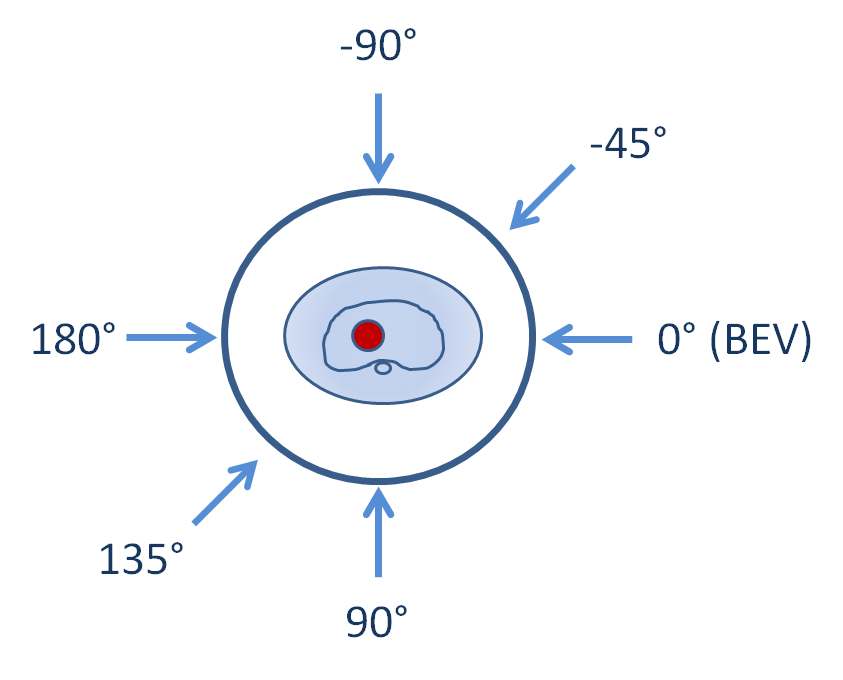
\includegraphics[scale=0.4]{GantryDirection_BEV.png}
  \caption{Entry channels for different gantry directions for a couch angle of 90$^{\circ}$. The beam's eye view (BEV) is marked.}
  \label{gantrydirection}
 \end{center}
\end{figure}


\newpage


\subsection{Treatment planning studies}

Besides representing a reference value for the 4D cases, 3D treatment plans were also generated here 
in order to find the best suited combinations of beam entry channels as well as to study possible safety margin limitations. In order to find 
a suitable field number and beam direction for the 4D treatment planning 
studies, static simulations on the original CTV volume (LPV together with RPV) with the above mentioned treatment planning parameters were 
carried out for all five patients. 17 different beam channel combinations were studied (see table \ref{tab:fields}). As a criteria for the 
best possible solution the dose to OAR were assessed. Furthermore, different ITV margins (original and increased with 3mm, 5mm and 7mm margin) 
were studied in 3D treatment plans for all patients. The resulting dose depositions were compared to dose deliveries with the same margins 
where the esophagus was included in the optimization process. Possible limitations were again analyzed according to the dose deposition in the OARs. \newline
\newline
In order to prepare for the 4D simulations, the motion of the PVs due to heartbeat was assessed. 
4D plans were distinguished between an underlying motion without any compensation, resulting in interplay patterns \cite{Phi92} \cite{Ber08}, 
and with the application of rescanning \cite{Phi92} as motion mitigation technique. For rescanning different rescan numbers 
(5, 10, 15 and 20) were compared. Static, interplay as well as rescanning treatment plans for all patients were carried out with one 
beam channel combination (couch angle of 90$^{\circ}$ and gantry angles of -45$^{\circ}$, 135$^{\circ}$ and 0$^{\circ}$), all four safety 
margins, the stated treatment planning parameters and the four stated motion trajectories. 


\subsection{Analysis}

Both the dose deposition in OAR as well as dose homogeneity in the target volume were studied. For the OAR dose-volume restriction in 
esophagus, trachea, aorta and the whole heart were compared to values from RTOG study protocols (see next paragraph). 
As further OARs cardiac substructures (ventricles and coronary arteries) were studied. 
For comparison of the resulting dose coverage in the target region dose-volume-histograms (DVHs) were studied. Furthermore 
motion-volume-histograms (MVHs) \cite{Ric13} were generated displaying the relative displacement of every voxel of the investigated volume to 
the reference phase in all three motion directions. With these values the resulting motion of the PVs due to heartbeat could be assessed. 

\newpage

\subsubsection{Dose-volume constraints for organs at risk}
\label{human:dose-volumeOar}
The dose deposition in the OAR is an important limitation and selection criteria when studying the field number and beam channel 
direction as well as the possible safety margin limitations. Since a single fraction of 25Gy or higher is assumed to be used in this 
non-invasive treatment modality, dose tolerance limits used in stereotactic body radiotherapy (SBRT) are highly related. An 
extensive collection of dose-volume-limits for SBRT are presented in Grimm et al. \cite{Gri11} and the AAPM Task Group Report \cite{AAPM10}.  
Both are literature reviews of limits utilized and reported in existing publications. For the OAR in the here presented 
treatment planning study (esophagus, trachea, heart and aorta) the dose-volume-limits in both literature reviews were taken from the 
Radiation Therapy Oncology Group (RTOG). The RTOG is a national clinical cooperative group of over 360 institutions across the United 
States and Canada, which was funded by the National Cancer Institute (NCI) \cite{RTOG}. In their study protocols RTOG 0631 
(a phase II/III trial of SBRT for localized spine metastasis) \cite{RTOG0631} and RTOG 0915 (a randomized phase II trial of SBRT for 
medically inoperable patients with stage I peripheral non-small cell lunger cancer) \cite{RTOG0915} the following dose-volume-limits 
were stated (see table \ref{tab:RTOG}). 

\vspace*{-1cm}

\begin{table}[H]
  \centering
  \footnotesize
  \caption{Dose-volume limits for OAR.}
  \begin{tabular}{|c|c|c|c|}
    \hline\hline
    OAR & Volume [cc] & Dose [Gy] & endpoint \\
    \hline
    Aorta / great vessels & 10 & 31 & Aneurysm \\
    Esophagus & 5 & 11.9 &  Stenosis / fistula \\
    Heart & 15 & 16 & Pericarditis \\
    Trachea & 4 & 10.5 & Stenosis / fistula \\
    \hline\hline
  \end{tabular}
  \label{tab:RTOG}
\end{table}

\vspace*{-0.3cm}

Since the heart is not only a critical organ but also the target site in this treatment modality, further differentiation of 
limits depending on the substructures of the heart are needed. Unfortunately, data on this topic is scarce. Literature on cardiac disease 
resulting from radiation exposure mostly relies on cancer patient data treated with radiotherapy (in particular breast cancer and Hodgkin's 
lymphoma) or atomic bomb survivors. Besides the stated dose-volume limitation, the mean dose and maximum point dose to the whole heart was 
studied. Furthermore the maximal irradiated heart volume (V$_{>0}$) was examined. 
Concerning substructures the left and right ventricle as well as the coronary arteries were analyzed for mean and maximum dose deposition and 
maximal irradiated volume contribution. Since the values were not normally distributed, boxplots were generated, where the median (50th 
percentile), the 25th and 75th percentile and the minimum and maximum values over all patient cases are displayed. 

\subsubsection{Dose deposition in target volume and motion of PVs}

The V95, V107 as well as D5-D95 of the CTVs were analyzed. 
The stated values have been evaluated for all beam applications (static, interplay, rescanning). 
Futhermore the median and percentile values of these parameters over all studied motion patterns and patient cases were 
generated. The relation of dose analysis parameters to different margin sizes and rescanning number was analyzed by a one-way ANOVA and 
the proportion of variance explained $r^{2}$ is reported with the corresponding p-value ($p$<0.0001). 


\vspace*{-0.3cm}

\section{Results}

In the following the results of the beam direction and safety margin study, PV motion assessment as well as the treatment planning studies 
will be discussed. As a criteria for an adequate field number and beam channel direction as well as safety margin limitation the dose to OAR 
will be presented. The motion due to heartbeat is shown. For the treatment planning study different dose analysis parameters will be presented 
and compared for different cases (static, interplay and rescanning). 

\vspace*{-0.3cm}

\subsection{Beam direction}

In figures \ref{beamdirection_boxplot} and \ref{beamdirection} the resulting dose to the pertinent OARs is shown for all studied beam 
directions and patients. Figure \ref{beamdirection_boxplot} displays the results as a boxplot over all patient cases for a respective field 
number (and hence different beam directions) while figure \ref{beamdirection} shows the individual results for each patient and beam direction. 
The corresponding volumes result from the dose volume limits (see table \ref{tab:RTOG}, represented by a dashed line in the plots). 
In all studied cases, the difference between different beam directions for a certain patient is rather small, resulting in no obvious 
preferable beam direction for the five studied patients. For the four studied OAR it becomes furthermore obvious, that while some organs, 
like trachea and aorta, are well spared for almost all beam directions in all patients, esophagus and in particular the heart are much more 
critical.\newline
\newline
In the esophagus the median dose over all patients is 7.8Gy (75th percentile: 9.0Gy) for one field, 11.0Gy (14.1Gy) for 
two fields, 11.0Gy (13.9Gy) for three and 8.0Gy (11.9Gy) for four fields. The result is dependent on the underlying patient anatomy. 
While the majority of the beam directions for patient 1, 4 and 5 remain under the respective dose-volume limit, many plans for patient 2 and 3 
exceed the dose-volume constraints. For these patients a dose deposition of 11.9Gy or less are achieved in only about 98\% and 65\% of 
studied cases (patient 2 and 3, respectively). While a single field yields acceptable dose deposition in the esophagus, the beam channel 
results in higher dose depositions in the heart and cardiac substructures like the coronary arteries (see 
figure \ref{beamdirection_MeanMaxD_MaxV} and \ref{beamdirection_MeanMaxD_MaxV_boxplot}) and are thus 
inapplicable. For patient 2 higher field numbers and thus more beam directions result in dose limit exceeding depositions. Due to this 
result the esophagus was included in the optimization of the treatment delivery (IMPT(OAR)). This was studied in comparison 
to a simple IMPT irradiation (see section \ref{safetymarginlimitation}).

%%%%%%%%%%%%%%%%%%%%%%%%%
%%%%%%%% DOSE TO OAR
%%%%%%%%%%%%%%%%%%%%%%%%%

\newpage

\vspace*{2cm}

\begin{figure}[H]
\subfigure[Esophagus]{
 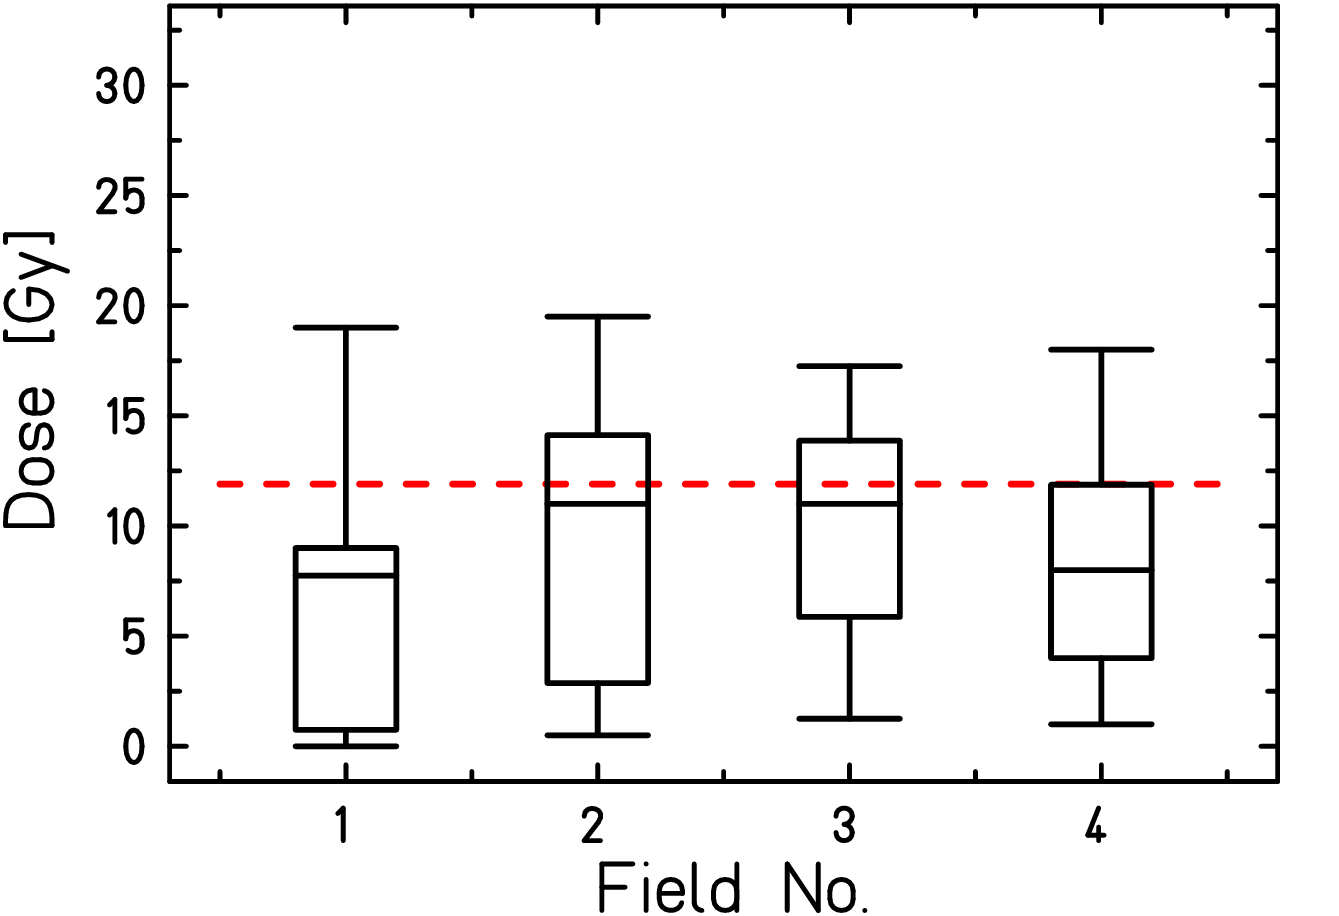
\includegraphics[scale=0.18]{Whisker_ESO.png}
 }
 \subfigure[Trachea]{
 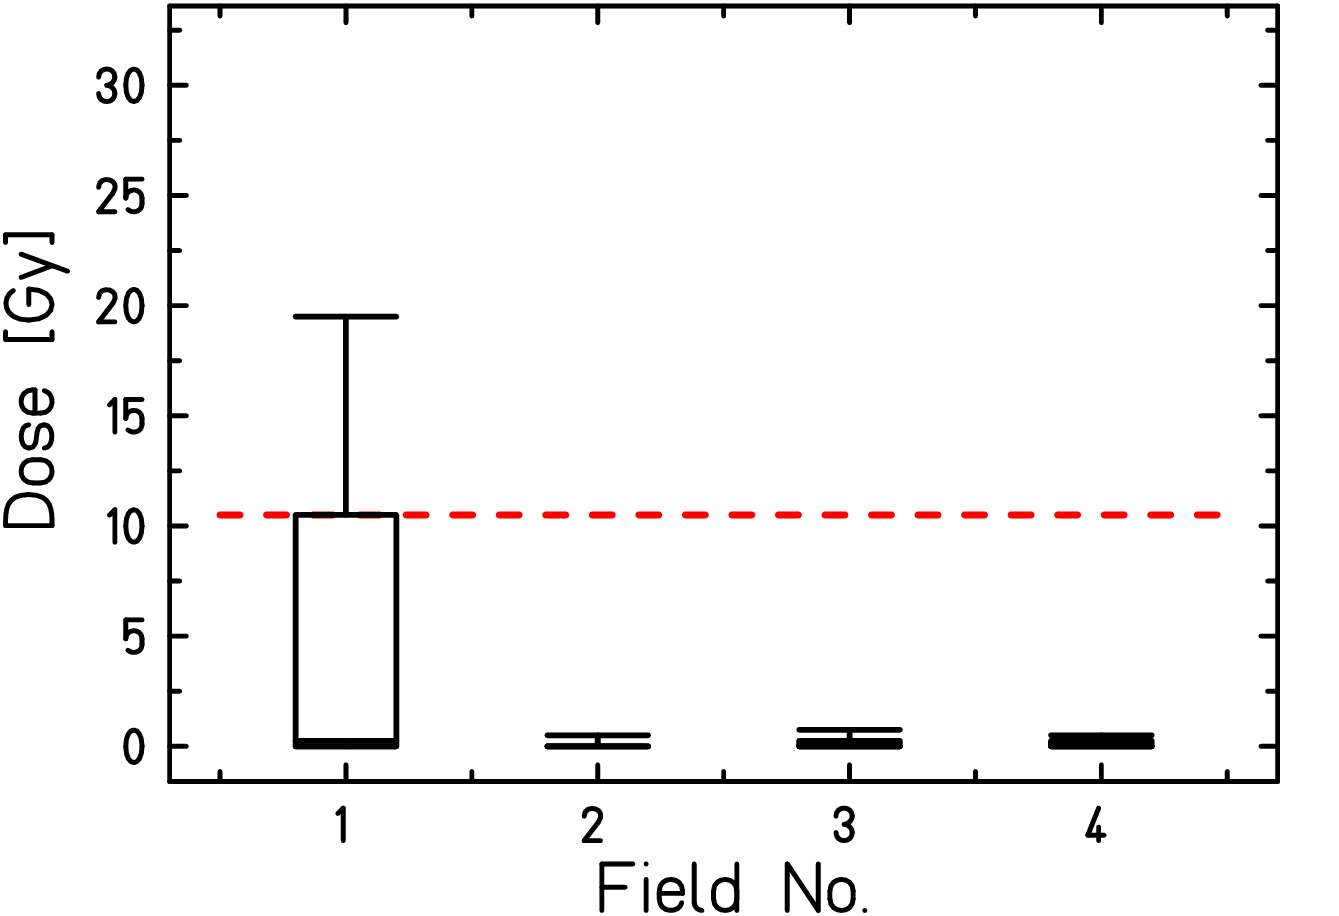
\includegraphics[scale=0.18]{Whisker_TRACHEA.png}
 }
  \subfigure[Heart]{
 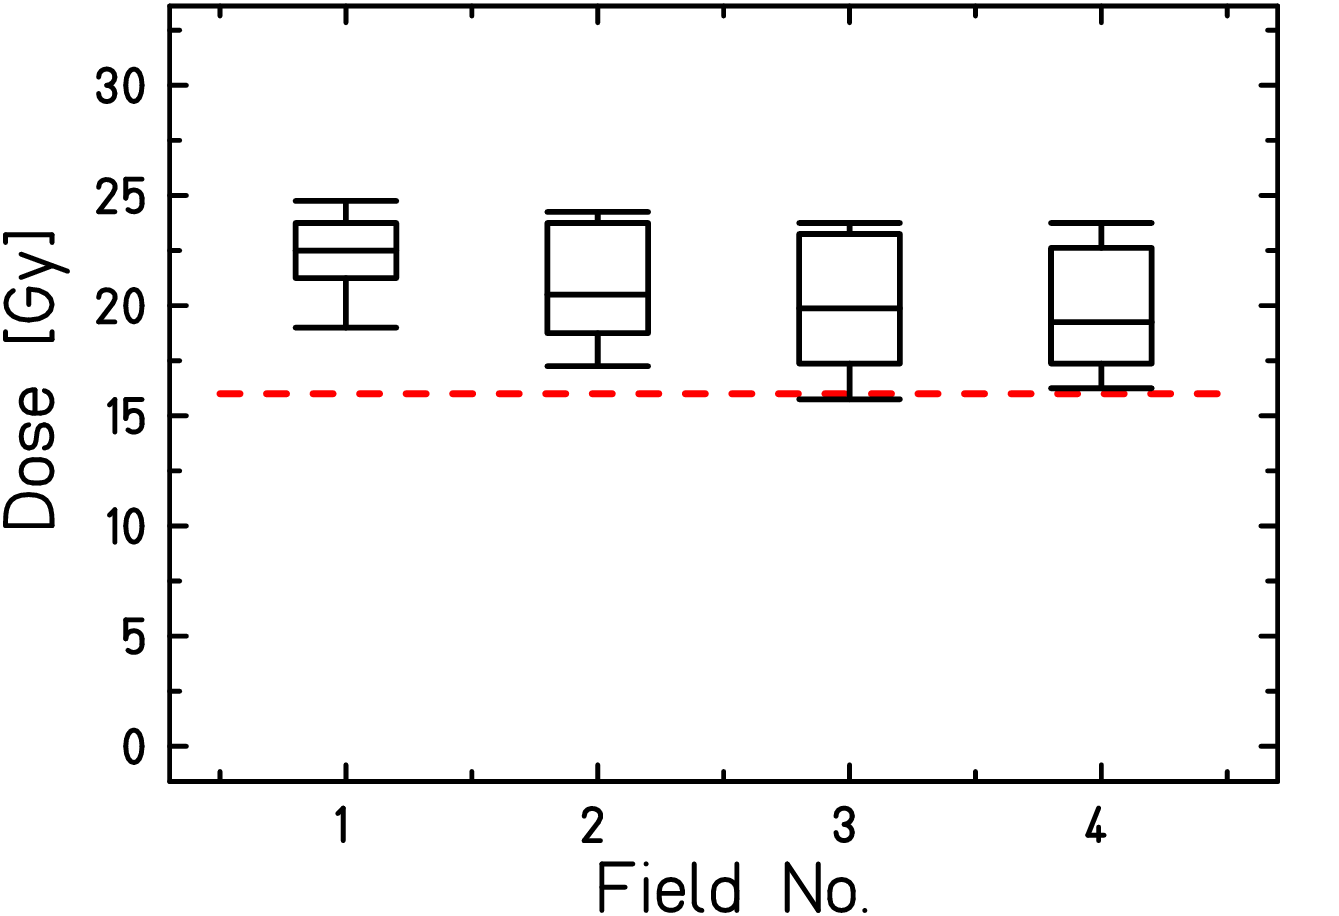
\includegraphics[scale=0.18]{Whisker_HEARTwoOverlap.png}
 }
  \subfigure[Aorta]{
 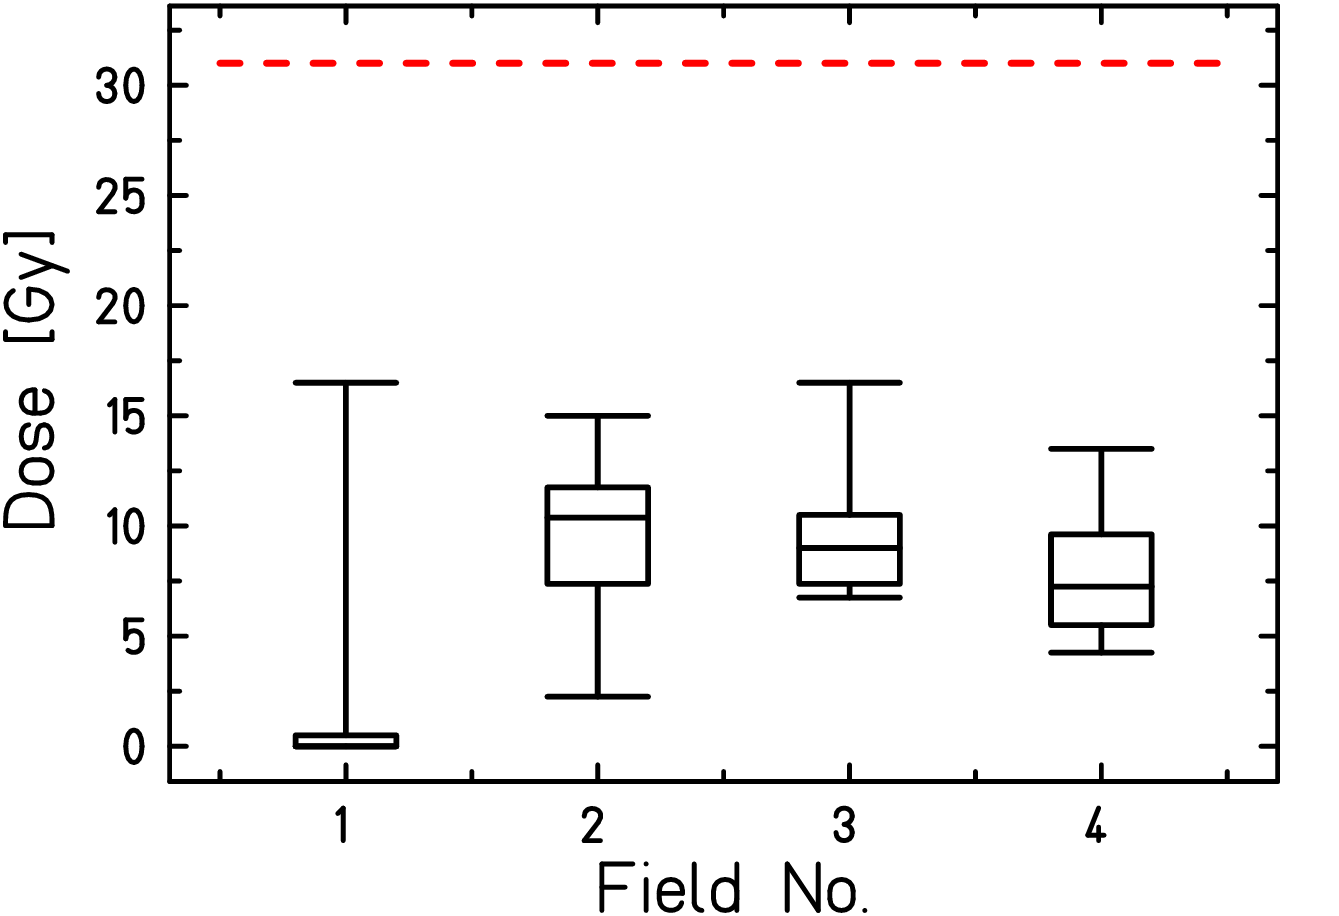
\includegraphics[scale=0.18]{Whisker_AORTA.png}
 }
\caption{Boxplots of dose-volume data for different field numbers (one to four fields) over all patients and over the 
respective beam directions. The data is plotted for different OARs when irradiating the LPV and RPV as IMPT in the five patient data sets. 
The dose-volume-limit for each critical organ is indicated with a dashed line in each plot, respectively.}
\label{beamdirection_boxplot}
\end{figure}

\newpage

% \vspace*{0.5cm}

\begin{figure}[H]
\subfigure[Esophagus]{
 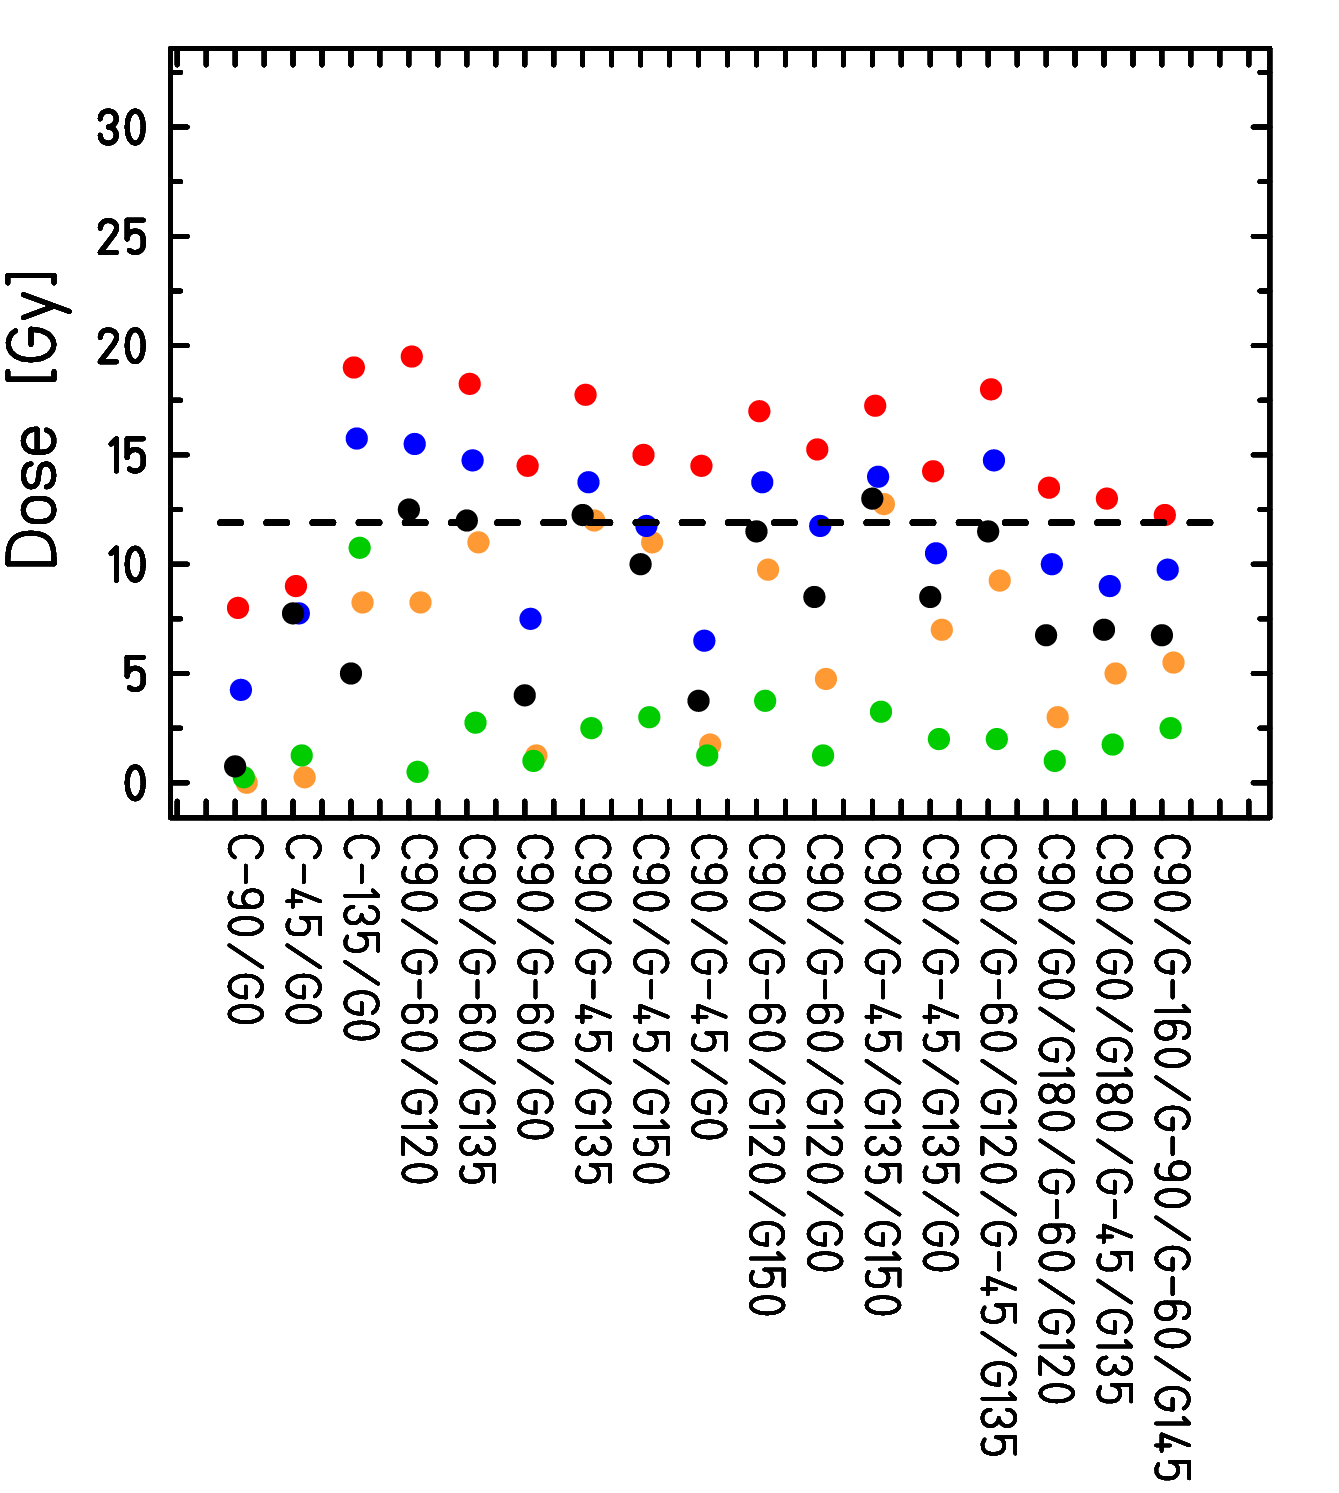
\includegraphics[scale=0.18]{Mayo_Human_BeamDirection_ESO.png}
 }
 \subfigure[Trachea]{
 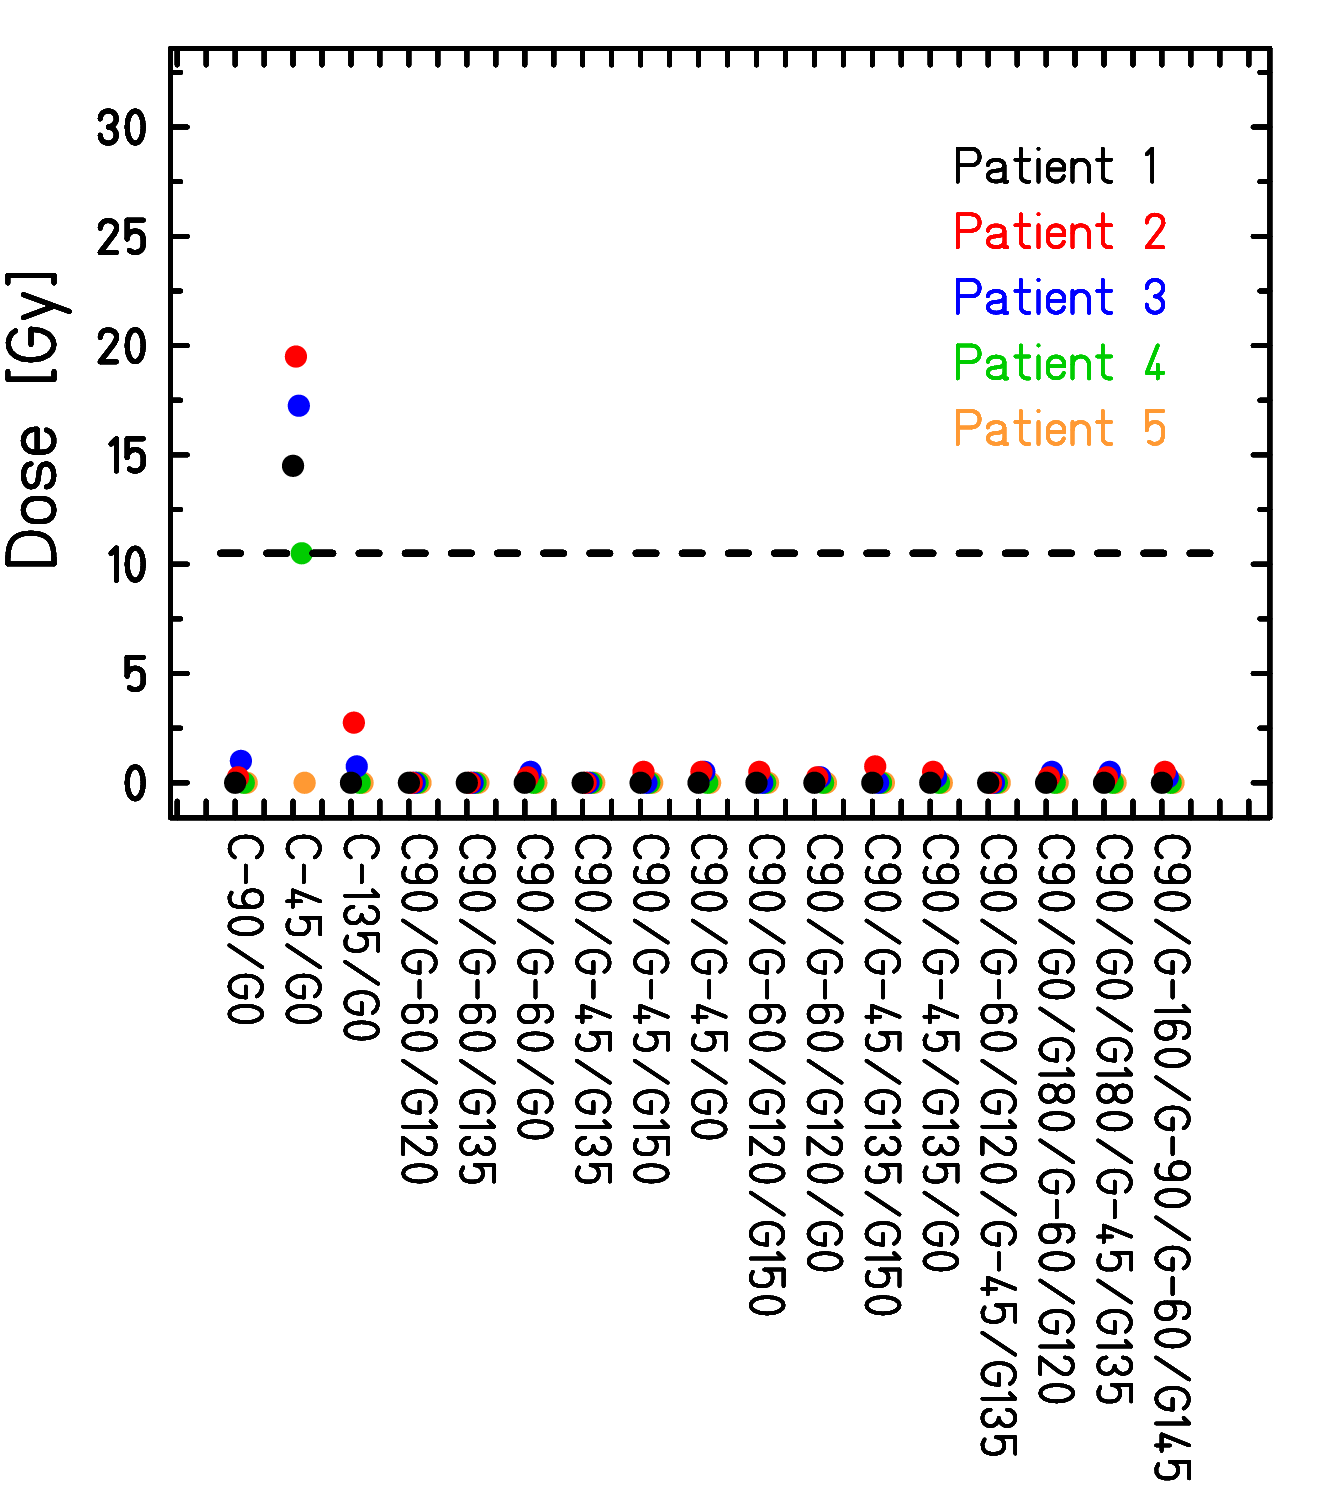
\includegraphics[scale=0.18]{Mayo_Human_BeamDirection_TRACHEA.png}
 }
  \subfigure[Heart]{
 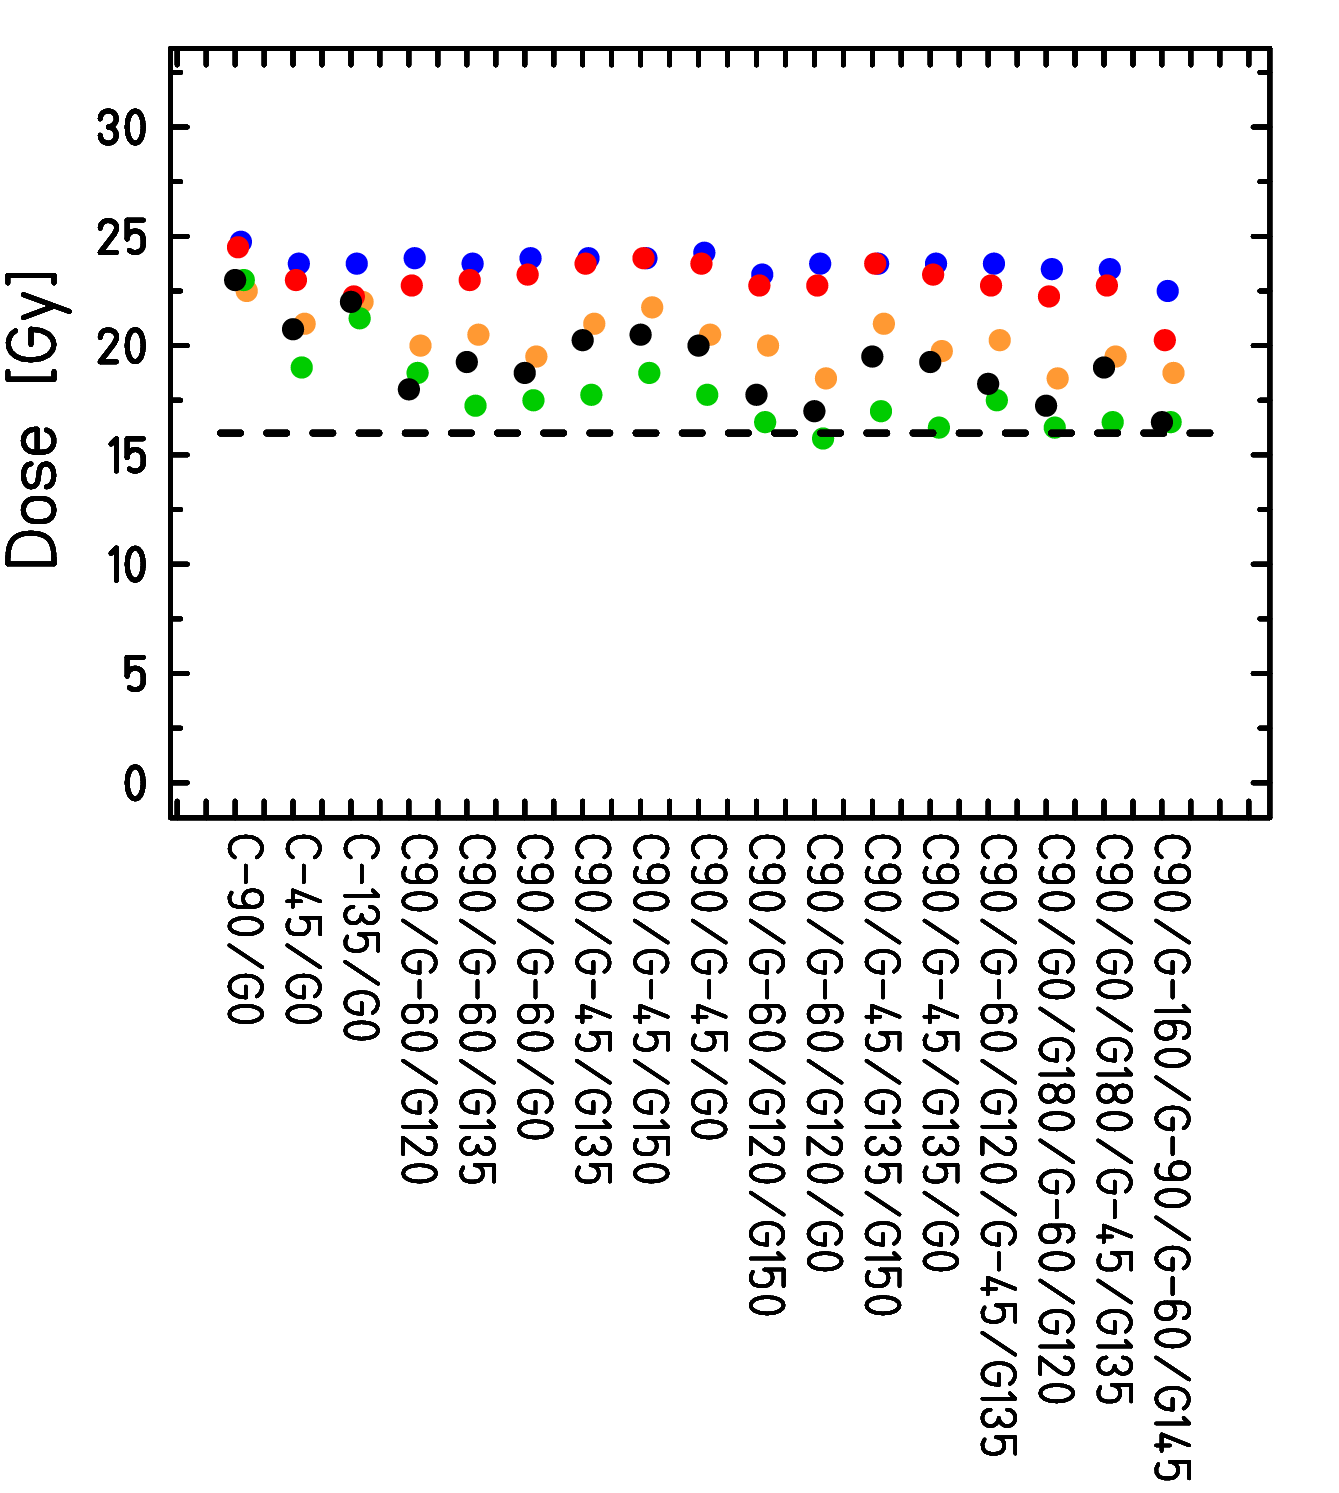
\includegraphics[scale=0.18]{Mayo_Human_BeamDirection_HEARTwoOverlap.png}
 }
  \subfigure[Aorta]{
 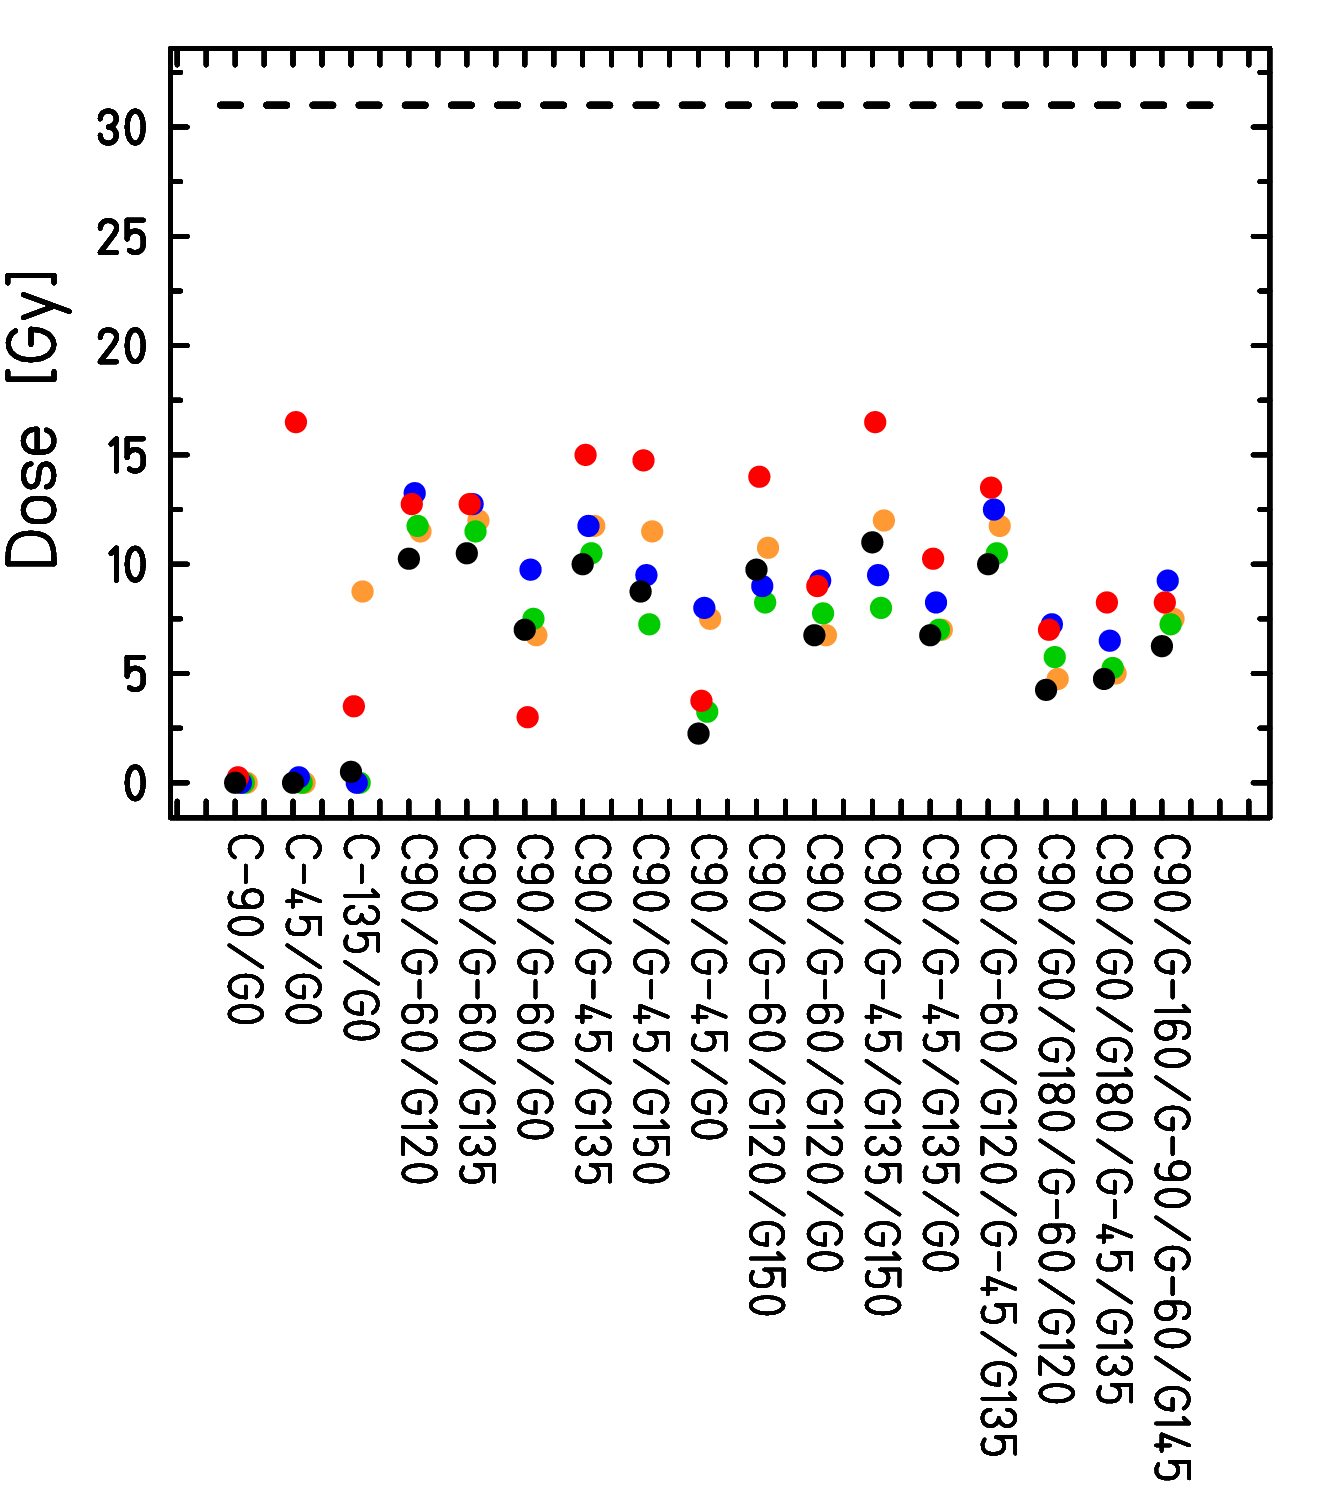
\includegraphics[scale=0.18]{Mayo_Human_BeamDirection_AORTA.png}
 }
\caption{Dose-volume data of different OAR when irradiating the LPV and RPV as IMPT in the five patient data sets (patient 1: black, 2: 
red, 3: blue, 4: green, 5: orange) with different field numbers (1 field, 2 fields, 3 fields, 4 fields) and different beam directions. 
The dose-volume-limit for each critical organ is indicated with a dashed line in each plot, respectively.}
\label{beamdirection}
\end{figure}

\newpage

The dose volume limit for the heart is exceeded in all patients for all beam directions (see figure \ref{beamdirection_boxplot} and \ref{beamdirection}. 
As the heart is not only an OAR in this treatment modality, but some of its substructures are also the target itself, a closer analysis of 
the dose deposition in the heart is required. In the first row of figure \ref{beamdirection_MeanMaxD_MaxV_boxplot} and figure \ref{beamdirection_MeanMaxD_MaxV} 
the mean and maximal dose deposition in the whole heart as well as the maximal irradiated volume are shown. The mean dose over all 
patients and beam directions is found to have a median of 1.3Gy (75th percentile: 1.5Gy). The median over the maximum point dose is 26.6Gy (27.1Gy).
Concerning the maximal irradiated volume it can be seen that except for one result less than 30\% of the heart is irradiated in all other cases. 
In the case of couch position 90$^{\circ}$ and gantry angles of -160$^{\circ}$, -90$^{\circ}$, -60$^{\circ}$ and 145$^{\circ}$ these maximal 
volume is drastically increased, and reaches up to 49.9\% for patient 2. Hence this beam channel case (beam channel case 17) will be 
stated separately in the following analysis. The median of the maximal irradiated volume over all patients is 16.8\% (20.5\%), 
excluding beam channel case 17, and 17.4\% (20.8\%) including this case.\newline
\newline
The results for the dose deposition in the cardiac substructures are presented in row two to five of figure \ref{beamdirection_MeanMaxD_MaxV_boxplot} and 
figure \ref{beamdirection_MeanMaxD_MaxV}. For the ventricles (LV: second row, RV: third row), the mean dose to both LV and RV is negligible. 
The maximal point dose on the other hand varies dependent on beam direction and patient. Single beam directions yield a high maximal dose 
deposition in the LV as in the case of a couch angle of -90$^{\circ}$ or -135$^{\circ}$ the beam traverses the LV. 
Thus for these beam directions the maximal dose to the RV is smaller. The overall maximal dose deposition has a median of 
1.4Gy (75th percentile: 7.4Gy) for LV and 1.3Gy (5.0Gy) for RV. Besides single beam directions no maximal point dose exceeds 11.2Gy and 10.1Gy 
for LV and RV, respectively. Concerning the maximal irradiated volume of the ventricles, it can be stated that the results differ depending on 
the studied patient. In case of the LV patient 2 has a higher irradiated volume compared to the other patients, while for this patient on the 
contrary the RV is better spared than in other patients. Over all patients the LV is irradiated to a higher extend than the RV. The maximal 
irradiated volume over all beam directions and patients has a median of 1.2\% (6.0\%) for LV, excluding the case of beam channel 17 and to 
1.9\% (6.4\%) including this case. For RV it is 0.2\% (7.6\%) excluding the beam channel case 17 and to 0.2\% (8.3\%) including it.
For the coronary arteries the beam channel 17 also results in the highest irradiated volume. 
Even though the coronary arteries are found on the surface of the whole heart and hence also on the ventricles, the irradiated volume of 
these structures differ from the result of the ventricles. Here the RCA are irradiated to a higher extent than the LCA. 
The median maximal value for the LCA is 15.7\% (28.0\%) including the stated beam channel case 17 and 15.2\% 
(27.4\%) excluding it. For the RCA the median over the maximal value is much higher and found to be 27.9\% (42.4\%) including the beam channel 
case 17 and to 24.8\% (42.1\%) excluding it. For the mean dose deposited in the LCA one and four beam directions result in an increased dose 
deposition, while three fields yield in general a low mean dose for all studied beam directions and patients. The same is true for the maximum 
point dose in the LCA. In the case of RCA, the resultS seem to be independent of field number and beam direction. Overall the median over the 
mean dose is 0.4Gy (1.0Gy) for LCA and 0.6Gy (1.6Gy) for RCA. For the maximal point dose the median dose deposition over all beam directions 
and patients is 6.8Gy (10.9Gy) for LCA. For the RCA it was found to be 5.4Gy (7.9Gy). \newline
\newline
While it was not expected to find one beam direction feasible for all five patients, it is striking that no beam position results in a clear 
benefit for the OAR of the individual patients. This is due to the challenging position of the PV target site, which is in direct proximity 
to the esophagus and due to the fact that the heart is not only an OAR in this treatment modality, but also the target site itself. 
Nevertheless for the analyzed cardiac substructure, especially the radiosensitive LCA, it can be concluded that three beam channels seem to be 
beneficial for all patients. Regarding the mean dose deposition in the LCA as well as the maximal irradiated heart volume, combined with the 
requirement of a robust treatment and hence the benefit of large gantry angles in between different beam channels, a couch angle of 
90$^{\circ}$ was chosen together with gantry angles of -45$^{\circ}$, 135$^{\circ}$ and 0$^{\circ}$. These beam channel directions were used 
for a closer analysis of safety margin limitation as well as for the treatment planning studies for all patients. 

\newpage

%%%%%%%%%%%%%%%%%%%%%%%%%
%%%%%%%% DOSE TO THE HEART
%%%%%%%%%%%%%%%%%%%%%%%%%

\begin{figure}[H]

\begin{minipage}{0.31\textwidth}
    \begin{overpic}
    [width=\textwidth]{Whisker_HEARTwoOverlap_MeanDose.png}
    \put(40,80){Heart}
    \end{overpic} 
\end{minipage}
\hfill
\begin{minipage}{0.31\textwidth}
  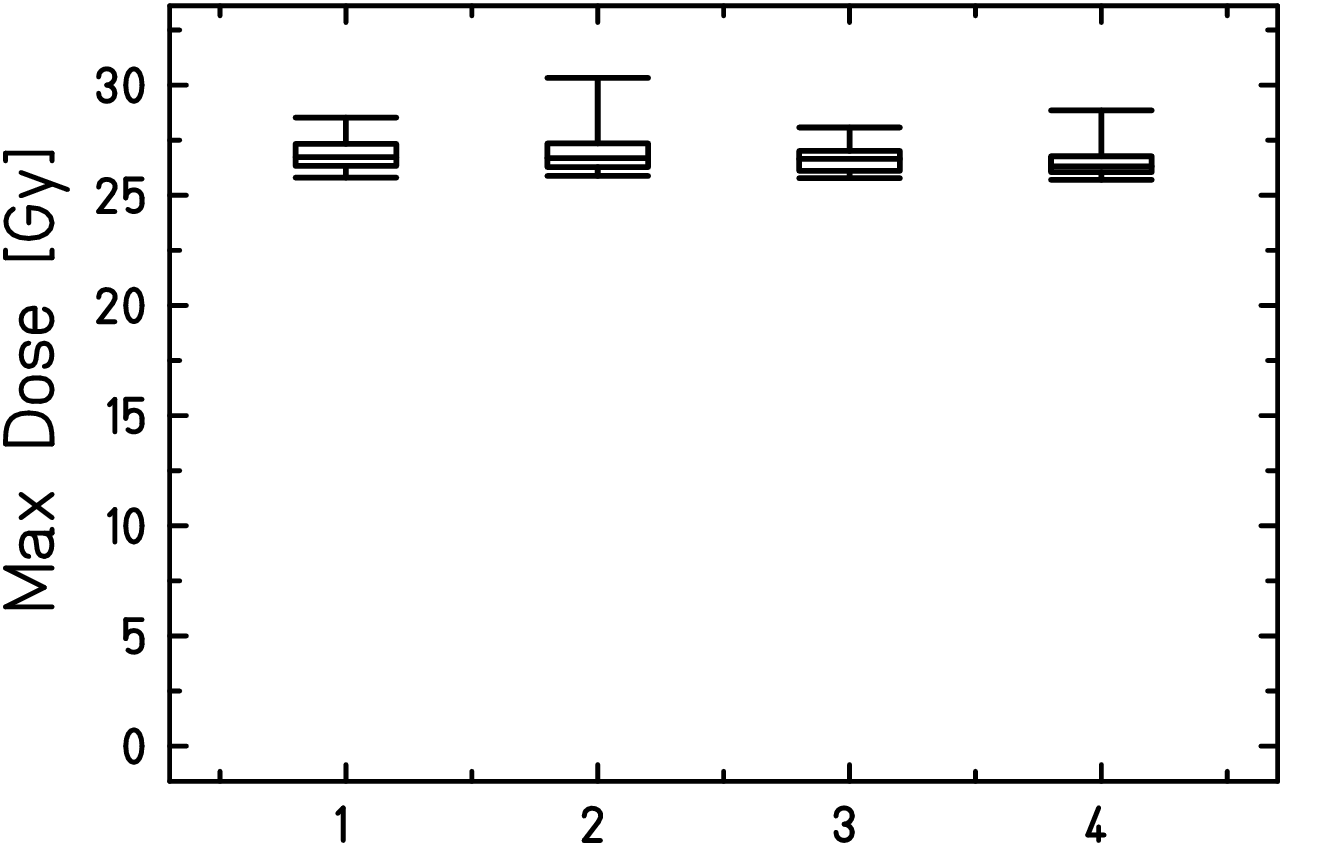
\includegraphics[width=\textwidth]{Whisker_HEARTwoOverlap_MaxDose.png}
\end{minipage}
\hfill
\begin{minipage}{0.31\textwidth}
  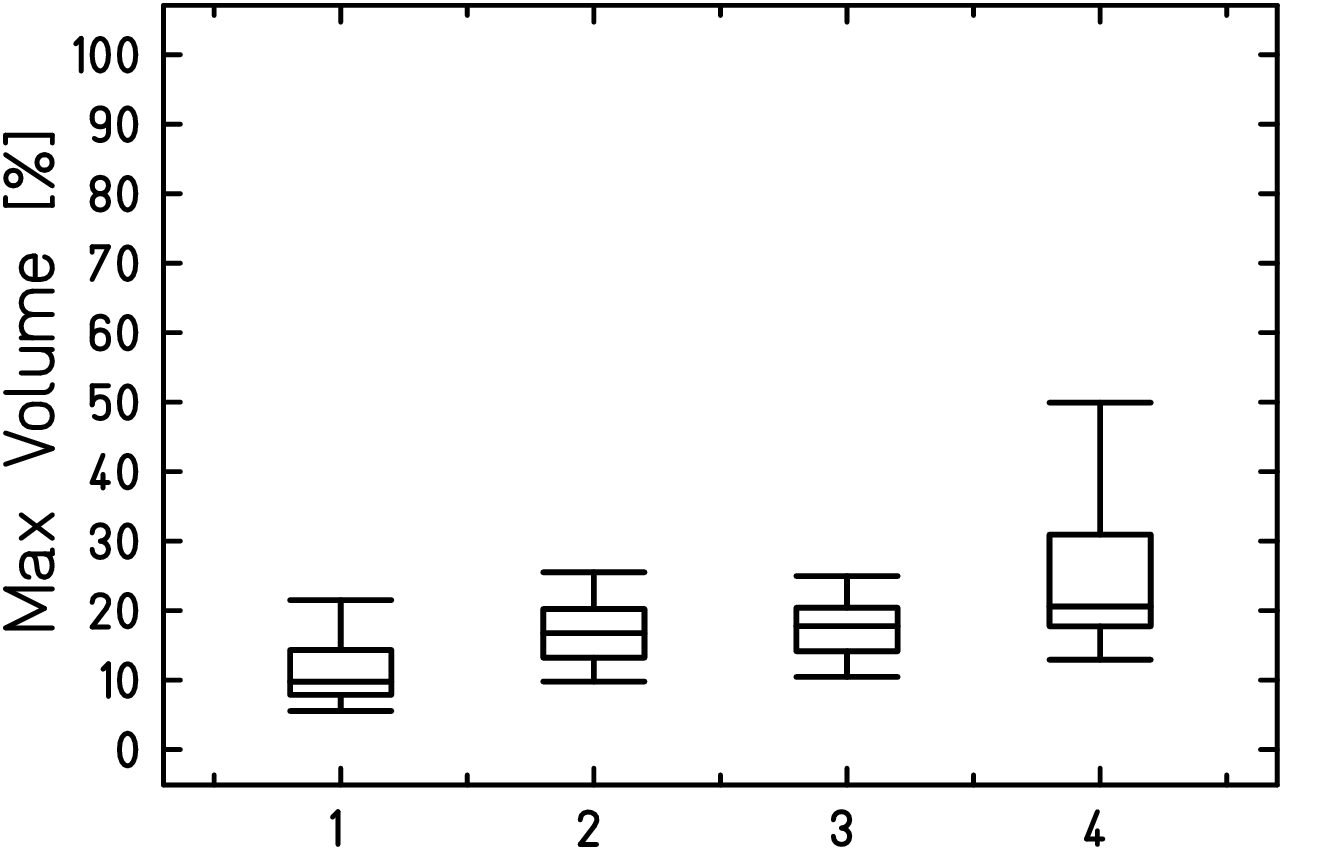
\includegraphics[width=\textwidth]{Whisker_HEARTwoOverlap_MaxVolume.png}
\end{minipage}

\hfill

\begin{minipage}{0.31\textwidth}
    \begin{overpic}
    [width=\textwidth]{Whisker_LV_MeanDose.png}
    \put(40,80){LV}
    \end{overpic} 
\end{minipage}
\hfill
\begin{minipage}{0.31\textwidth}
  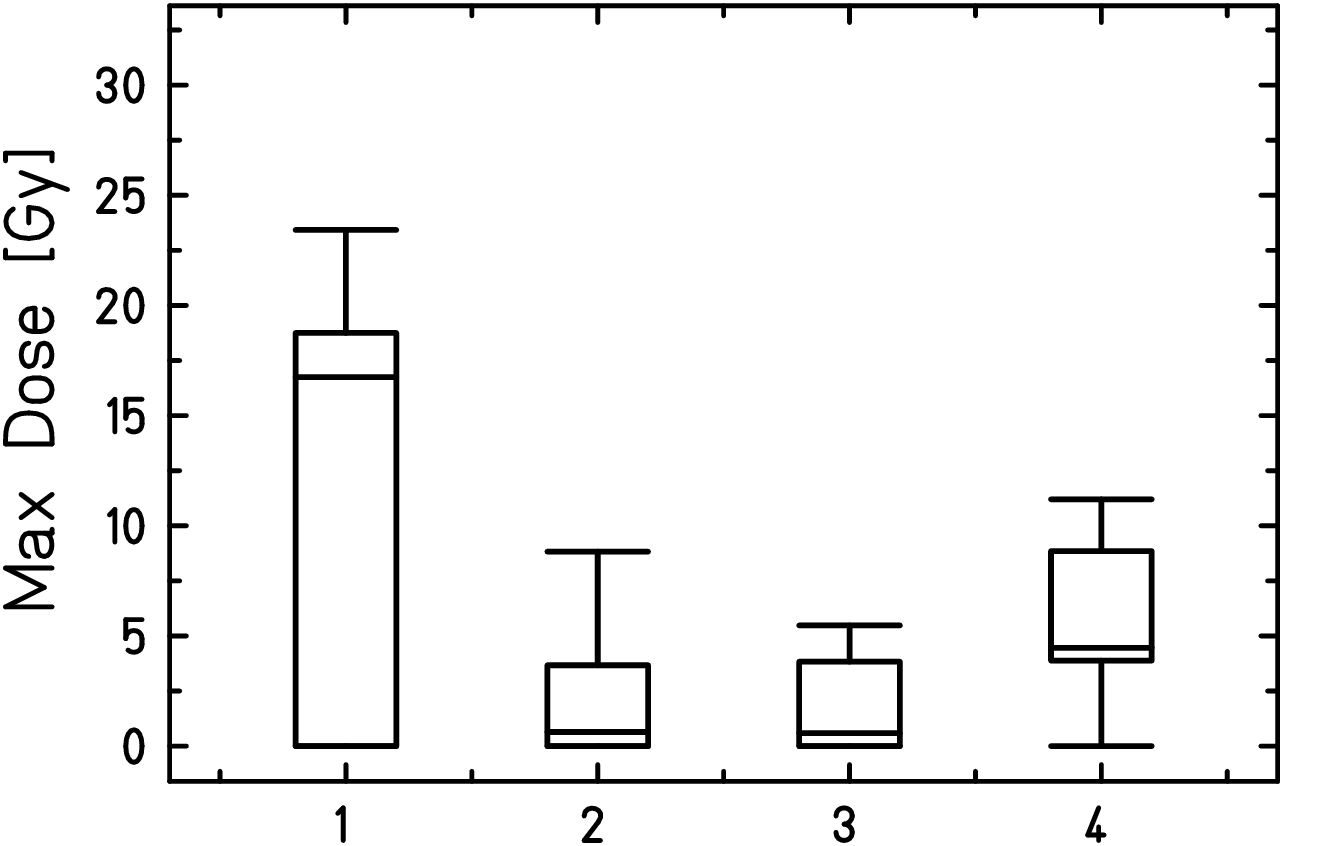
\includegraphics[width=\textwidth]{Whisker_LV_MaxDose.png}
\end{minipage}
\hfill
\begin{minipage}{0.31\textwidth}
  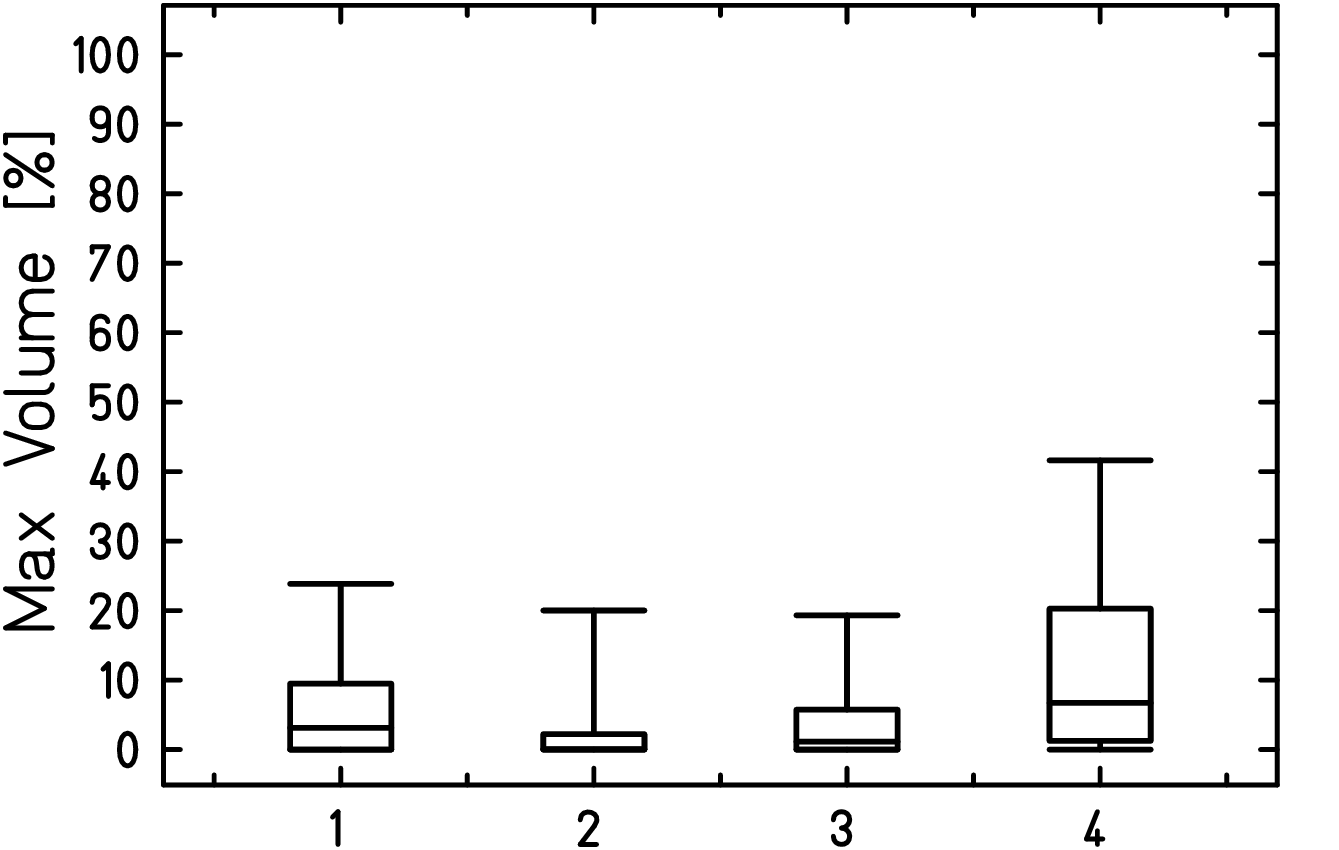
\includegraphics[width=\textwidth]{Whisker_LV_MaxVolume.png}
\end{minipage}

\hfill

\begin{minipage}{0.31\textwidth}
    \begin{overpic}
    [width=\textwidth]{Whisker_RV_MeanDose.png}
    \put(40,80){RV}
    \end{overpic} 
\end{minipage}
\hfill
\begin{minipage}{0.31\textwidth}
  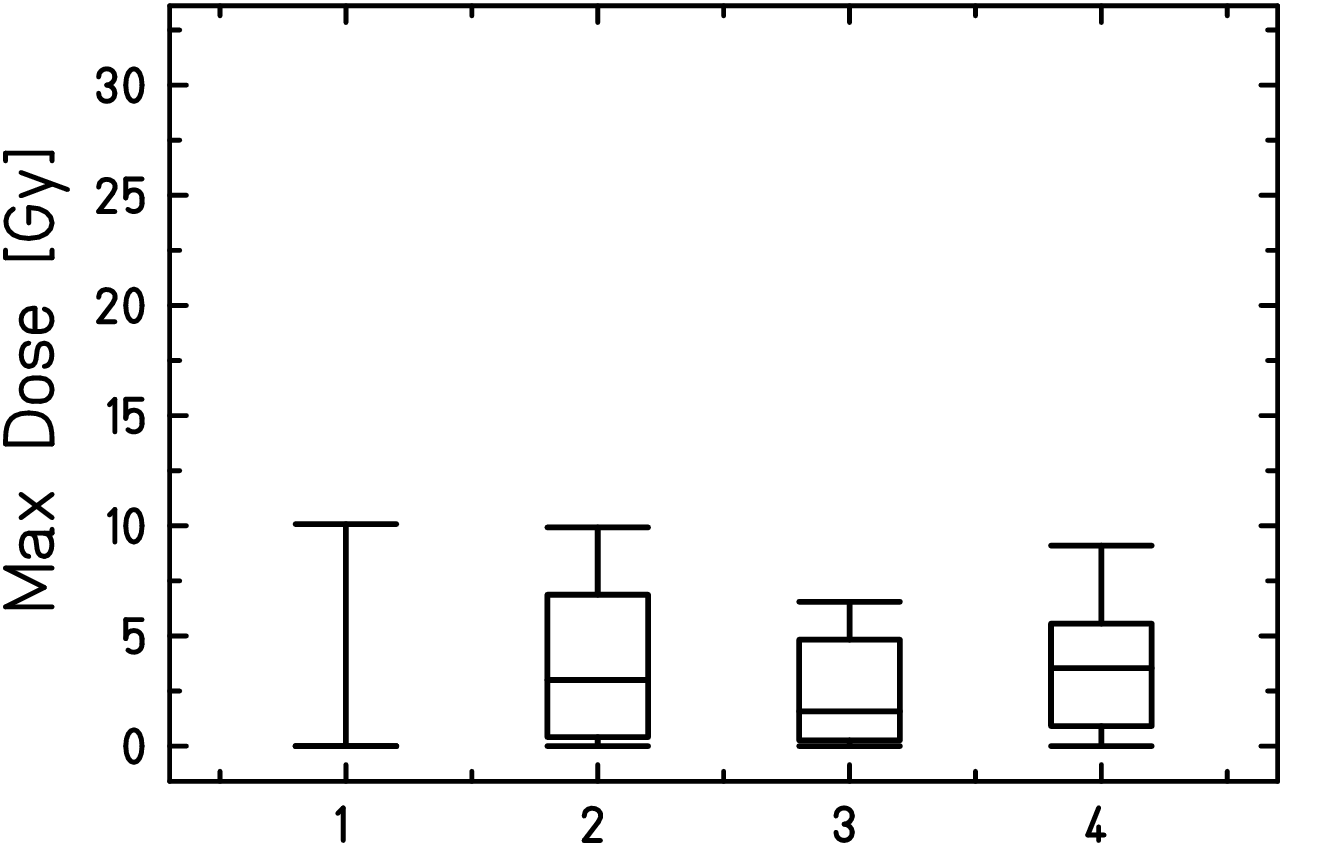
\includegraphics[width=\textwidth]{Whisker_RV_MaxDose.png}
\end{minipage}
\hfill
\begin{minipage}{0.31\textwidth}
  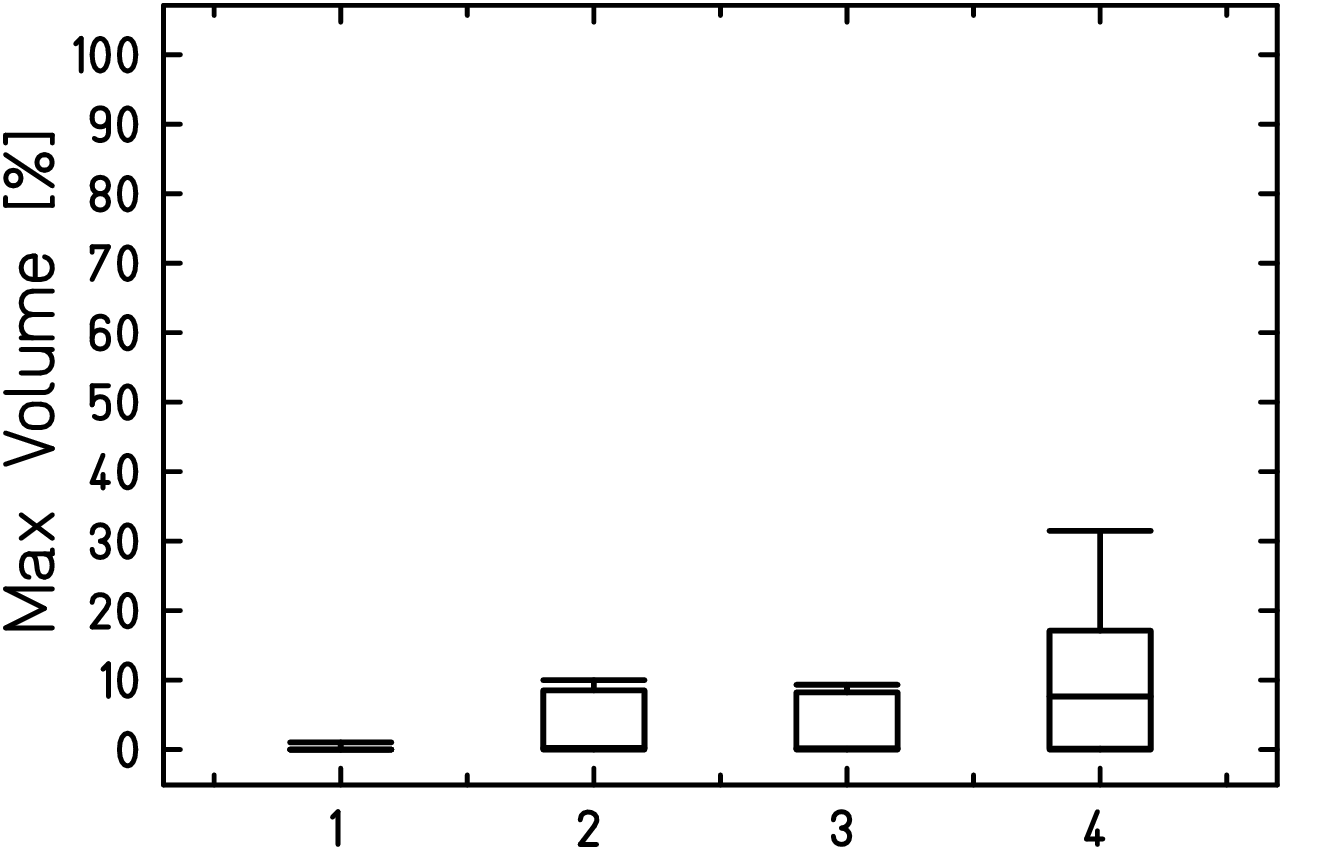
\includegraphics[width=\textwidth]{Whisker_RV_MaxVolume.png}
\end{minipage}

\hfill

\begin{minipage}{0.31\textwidth}
    \begin{overpic}
    [width=\textwidth]{Whisker_LCA_MeanDose.png}
    \put(40,80){LCA}
    \end{overpic} 
\end{minipage}
\hfill
\begin{minipage}{0.31\textwidth}
  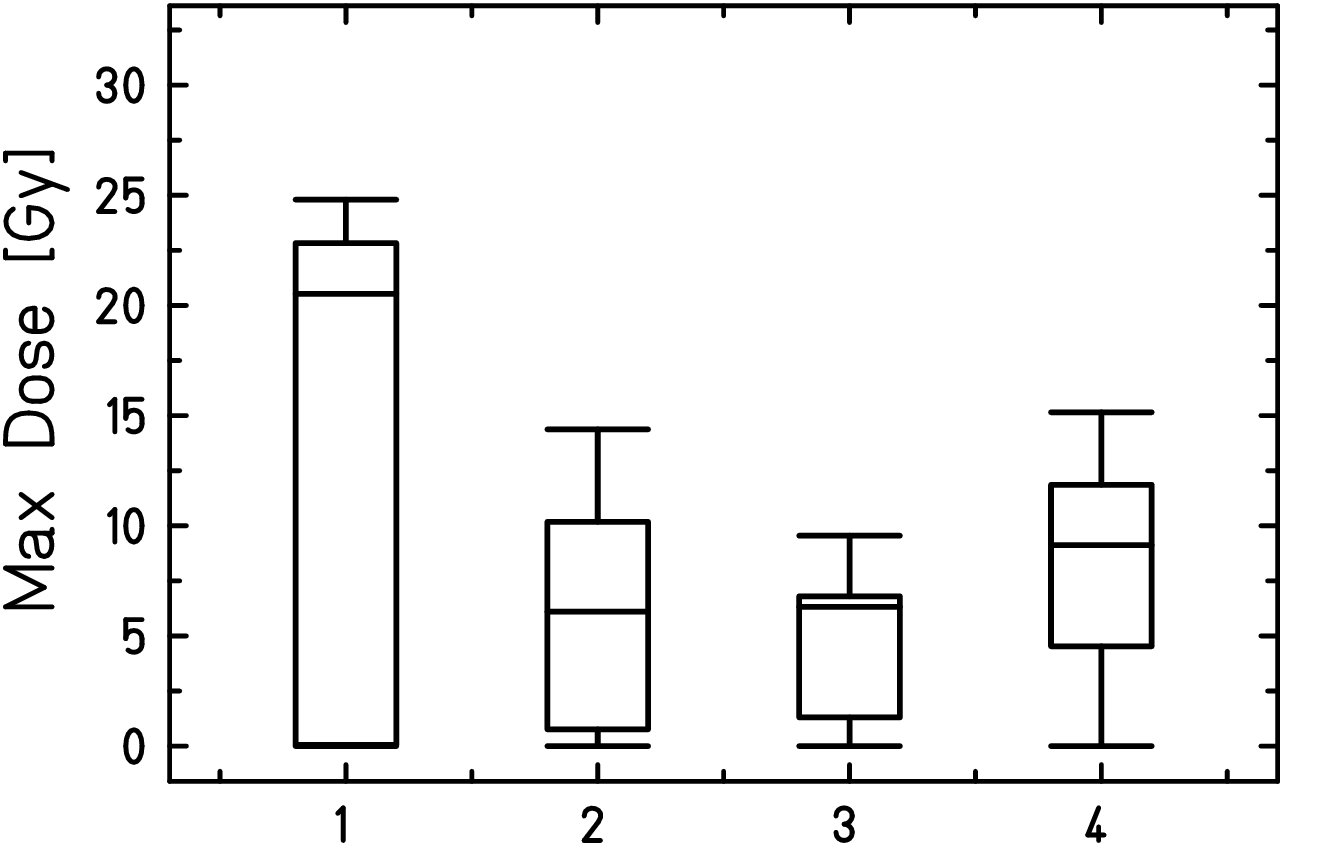
\includegraphics[width=\textwidth]{Whisker_LCA_MaxDose.png}
\end{minipage}
\hfill
\begin{minipage}{0.31\textwidth}
  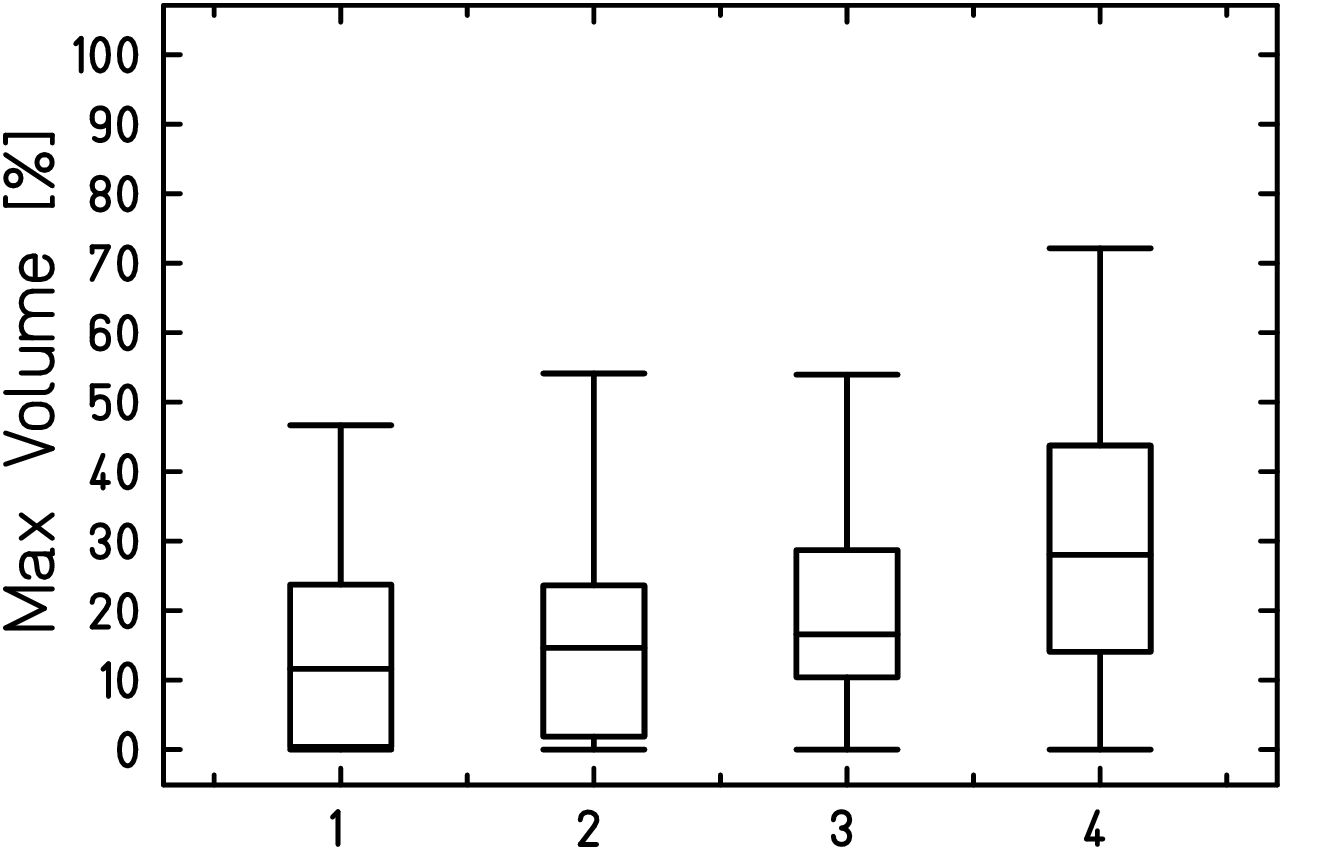
\includegraphics[width=\textwidth]{Whisker_LCA_MaxVolume.png}
\end{minipage}

\hfill

\begin{minipage}{0.31\textwidth}
    \begin{overpic}
    [width=\textwidth]{Whisker_RCA_MeanDose.png}
    \put(40,90){RCA}
    \end{overpic} 
\end{minipage}
\hfill
\begin{minipage}{0.31\textwidth}
  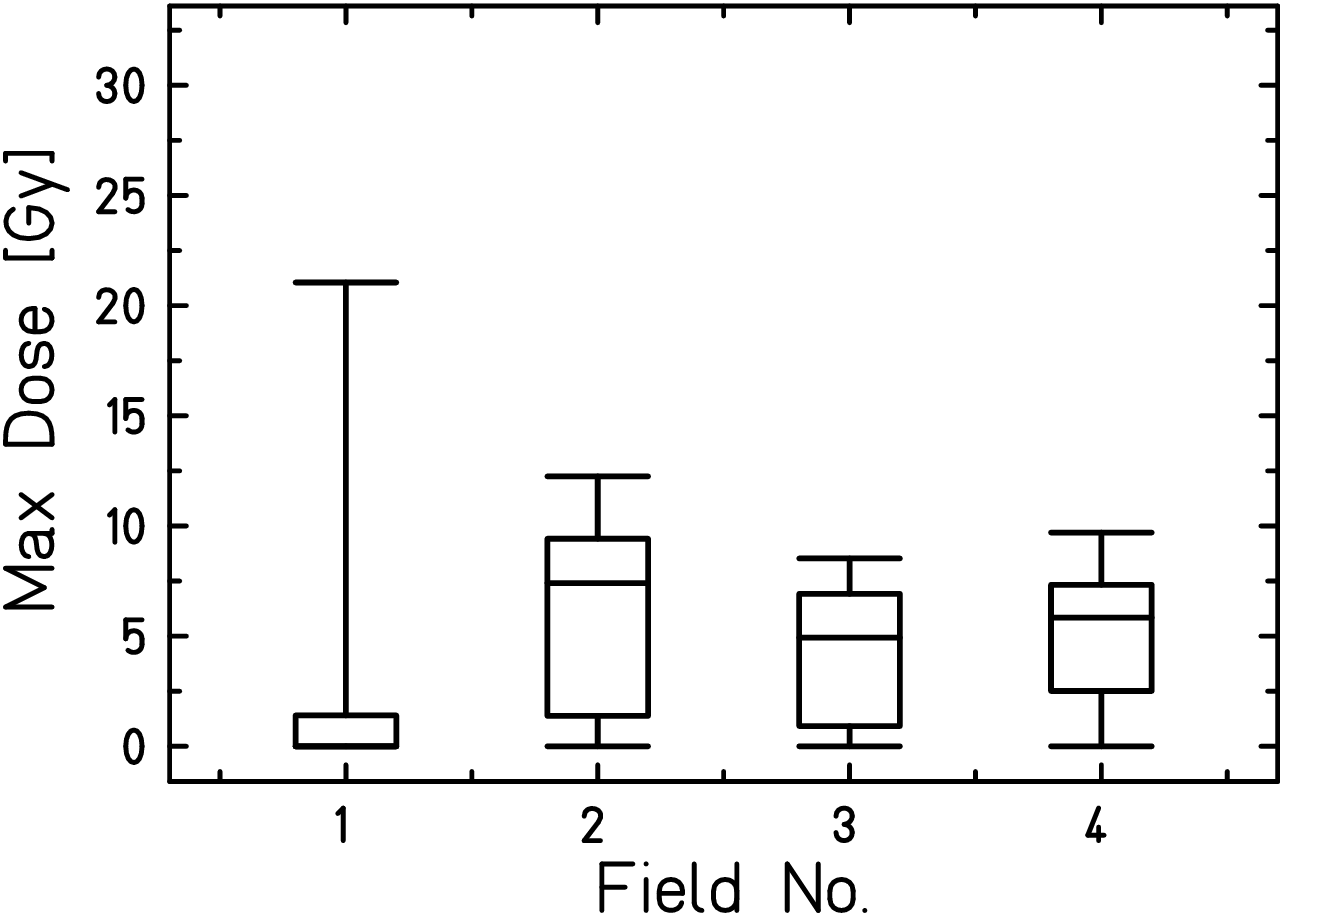
\includegraphics[width=\textwidth]{Whisker_RCA_MaxDose.png}
\end{minipage}
\hfill
\begin{minipage}{0.31\textwidth}
  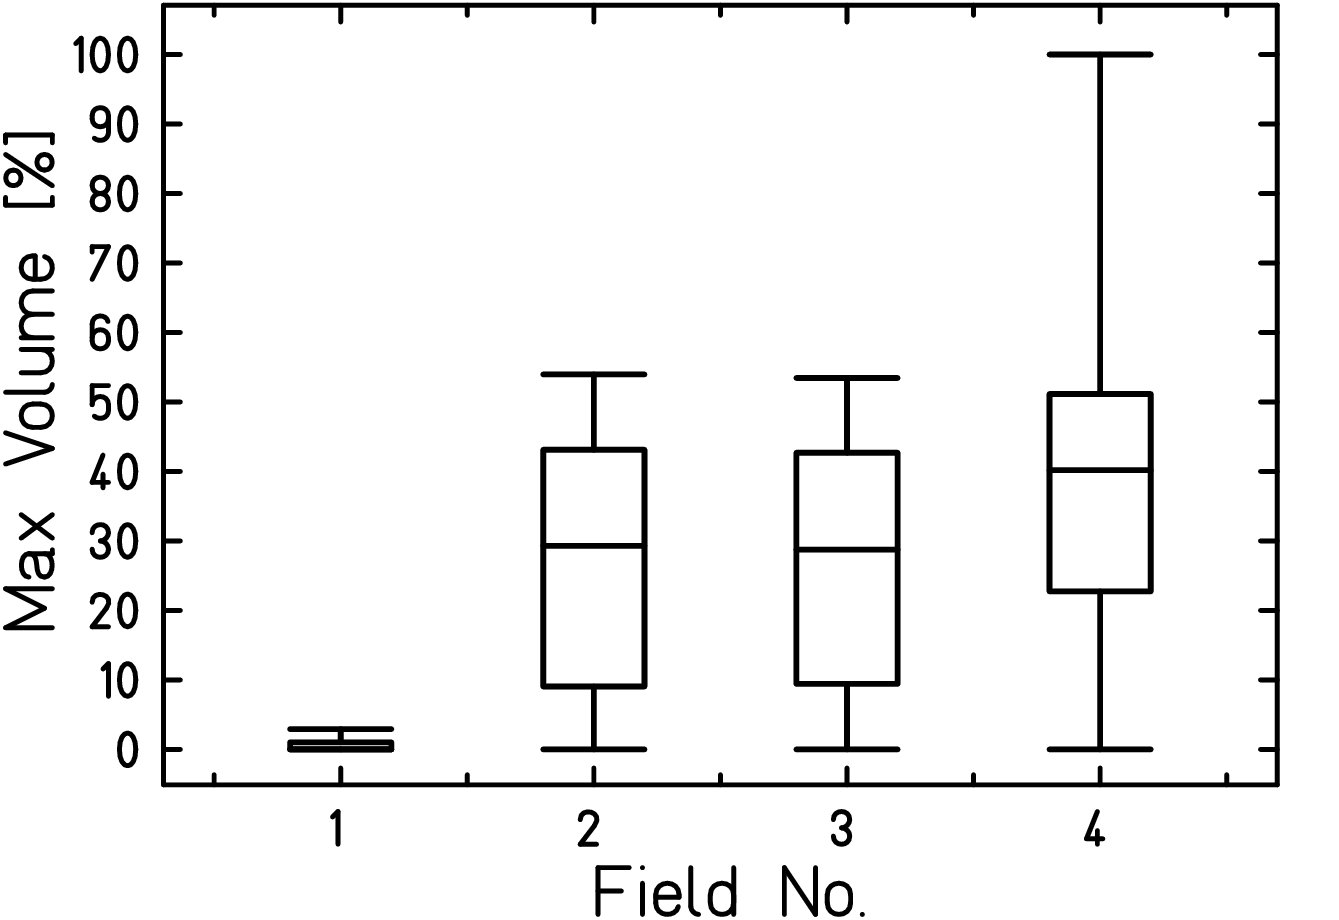
\includegraphics[width=\textwidth]{Whisker_RCA_MaxVolume.png}
\end{minipage}

  \caption{Boxplots of mean and maximum dose as well as maximal irradiated volume for different field numbers (one to four fields) over all 
  patients and over the respective beam directions. The data is plotted for different OARs (heart: first row, 
  and cardiac substructures (LV: second row, RV: third row, LCA: fourth row, RCA: last row) when irradiating the LPVs and RPVs as IMPT 
  treatment in the five patient data sets with different field numbers and thus beam directions.}
  \label{beamdirection_MeanMaxD_MaxV_boxplot}
  
\end{figure}



\begin{figure}[H]

\begin{minipage}{0.31\textwidth}
    \begin{overpic}
    [width=\textwidth]{Mayo_Human_BeamDirection_HEARTwoOverlap_MeanDose.png}
    \put(40,80){Heart}
    \end{overpic} 
\end{minipage}
\hfill
\begin{minipage}{0.31\textwidth}
  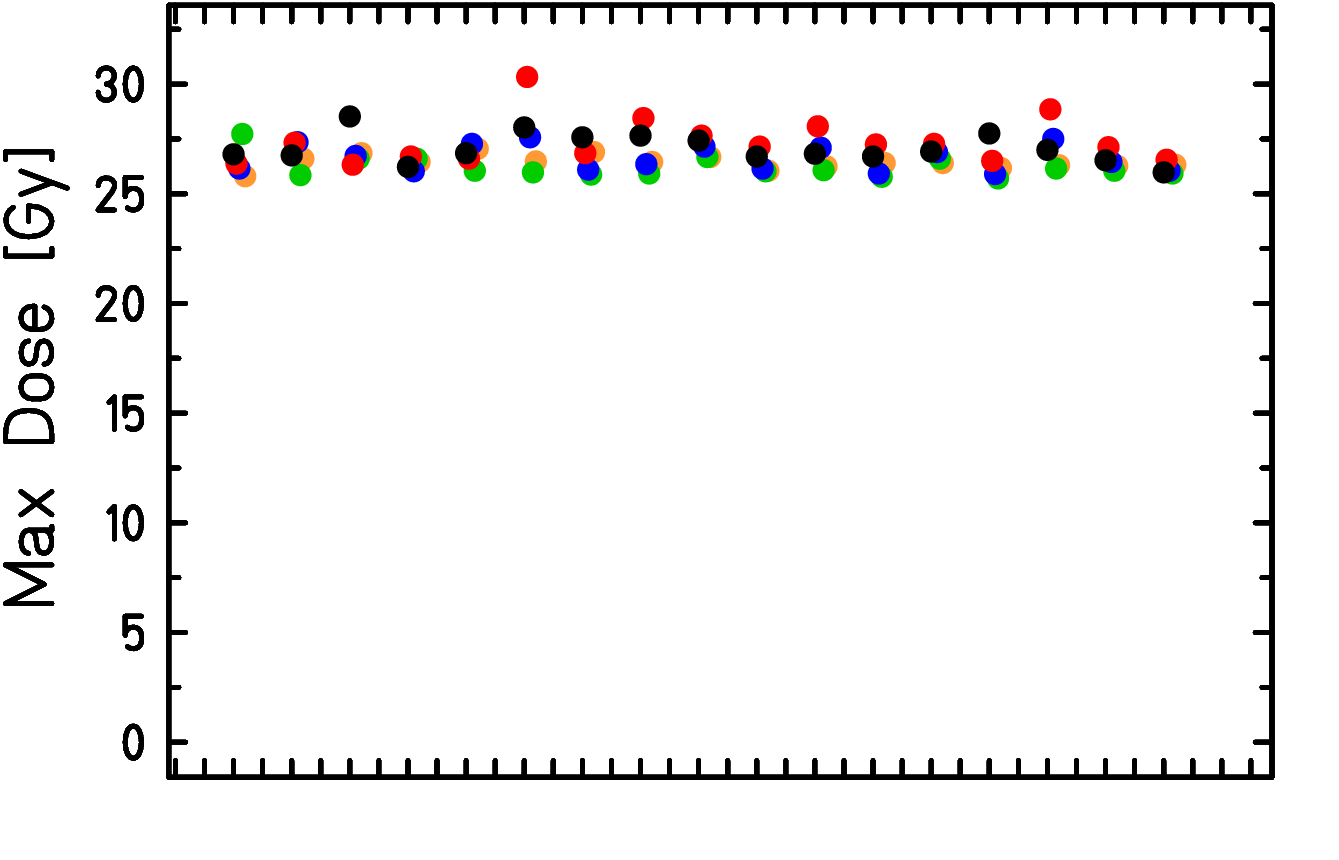
\includegraphics[width=\textwidth]{Mayo_Human_BeamDirection_HEARTwoOverlap_MaxDose.png}
\end{minipage}
\hfill
\begin{minipage}{0.31\textwidth}
  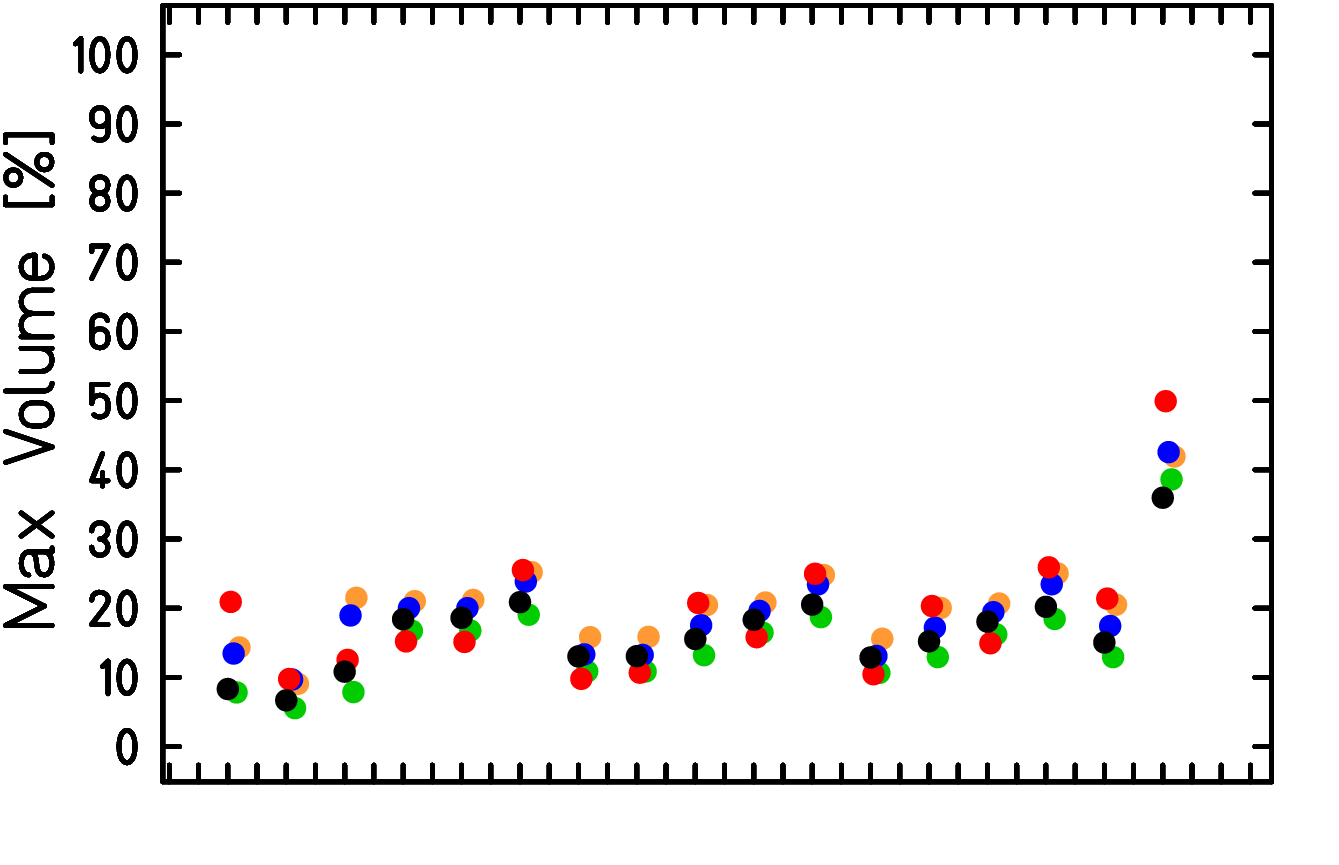
\includegraphics[width=\textwidth]{Mayo_Human_BeamDirection_HEARTwoOverlap_MaxVolume.png}
\end{minipage}

\hfill

\begin{minipage}{0.31\textwidth}
    \begin{overpic}
    [width=\textwidth]{Mayo_Human_BeamDirection_LV_MeanDose.png}
    \put(40,80){LV}
    \end{overpic} 
\end{minipage}
\hfill
\begin{minipage}{0.31\textwidth}
  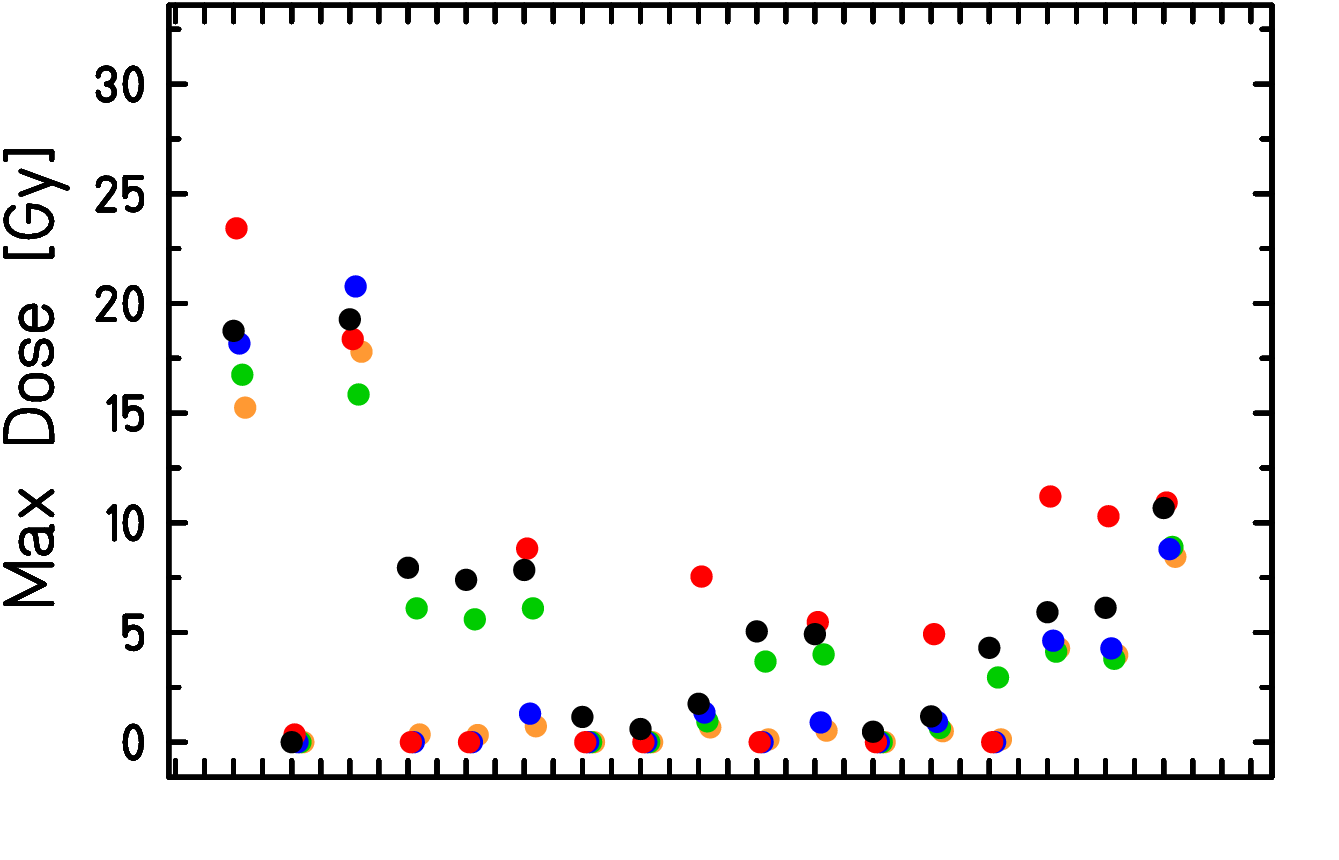
\includegraphics[width=\textwidth]{Mayo_Human_BeamDirection_LV_MaxDose.png}
\end{minipage}
\hfill
\begin{minipage}{0.31\textwidth}
  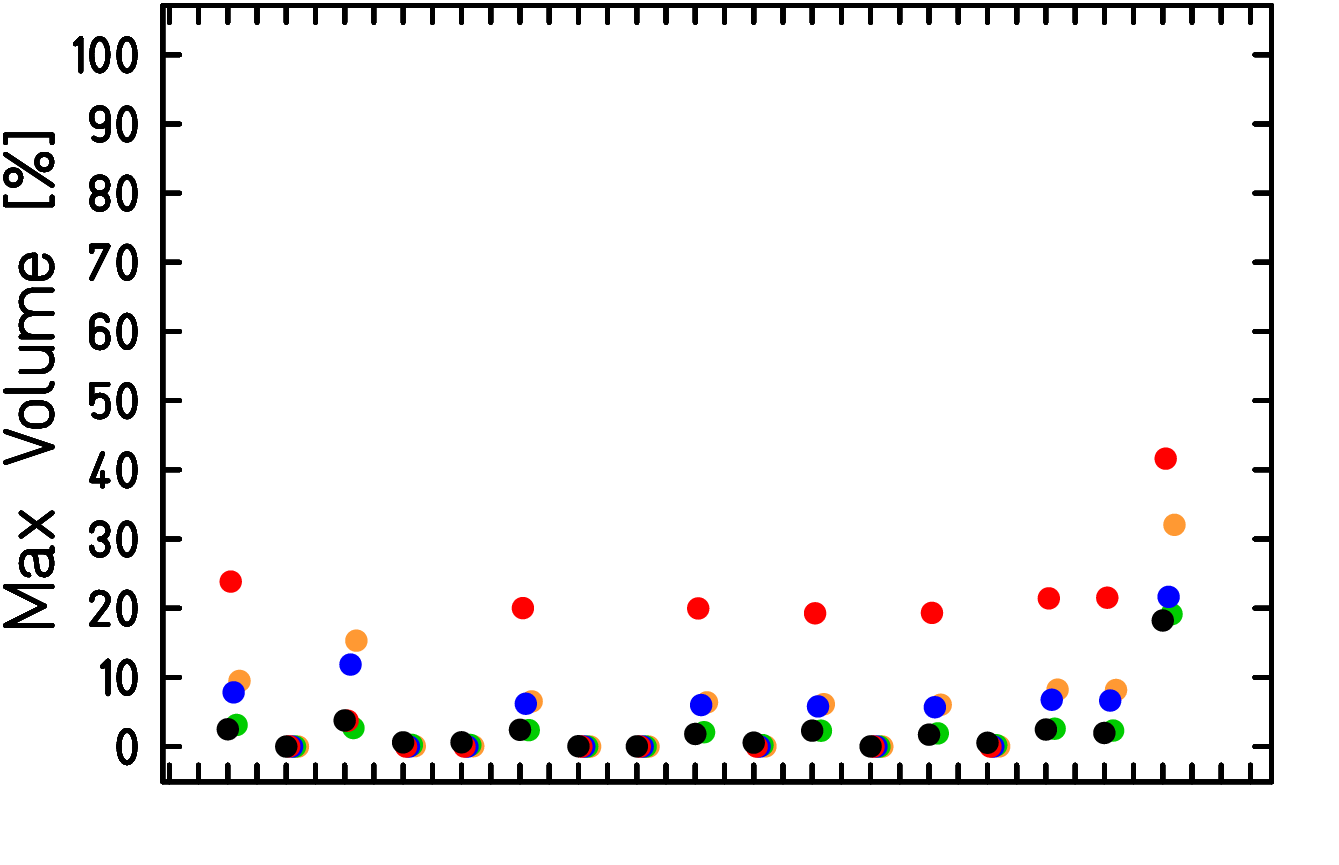
\includegraphics[width=\textwidth]{Mayo_Human_BeamDirection_LV_MaxVolume.png}
\end{minipage}


\hfill

\begin{minipage}{0.31\textwidth}
    \begin{overpic}
    [width=\textwidth]{Mayo_Human_BeamDirection_RV_MeanDose.png}
    \put(40,80){RV}
    \end{overpic} 
\end{minipage}
\hfill
\begin{minipage}{0.31\textwidth}
  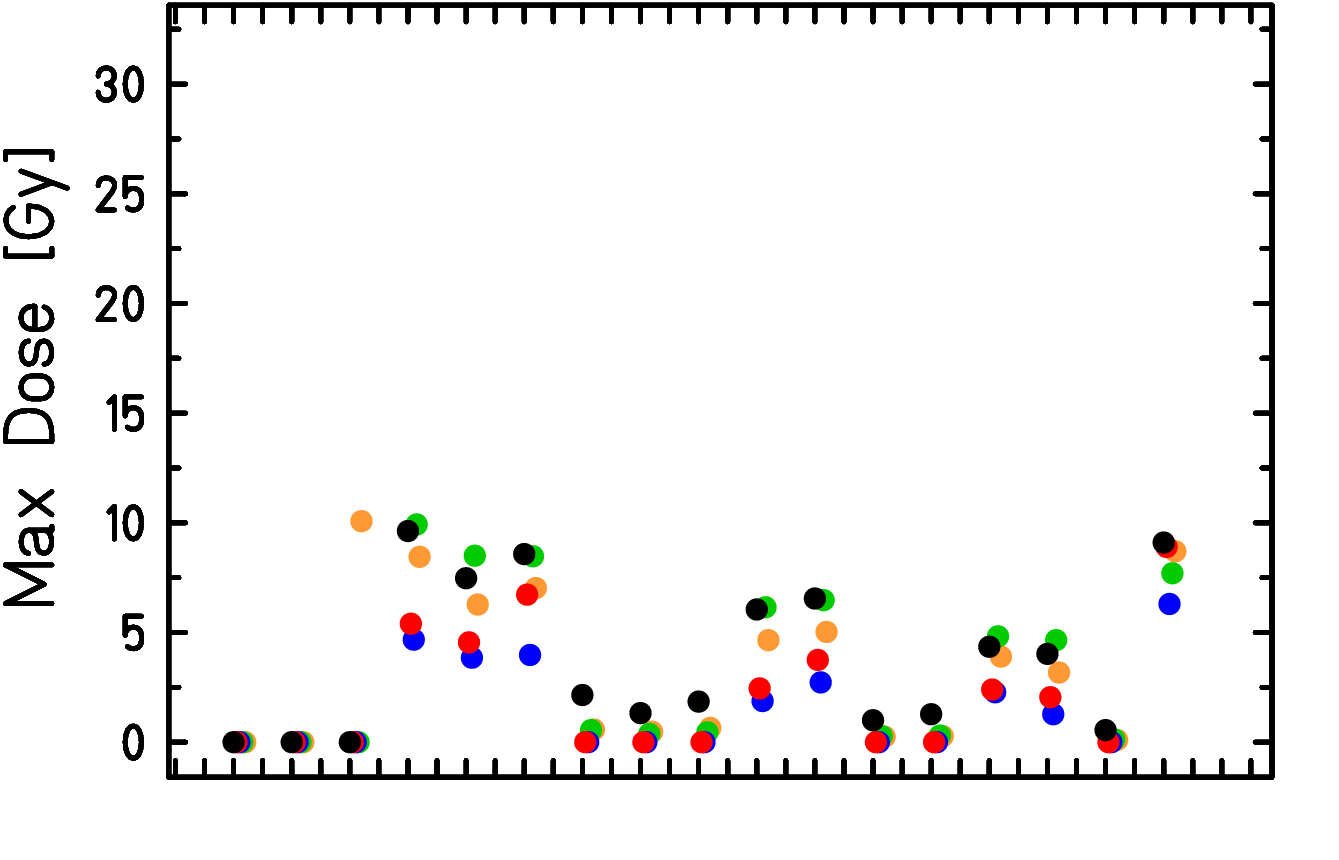
\includegraphics[width=\textwidth]{Mayo_Human_BeamDirection_RV_MaxDose.png}
\end{minipage}
\hfill
\begin{minipage}{0.31\textwidth}
  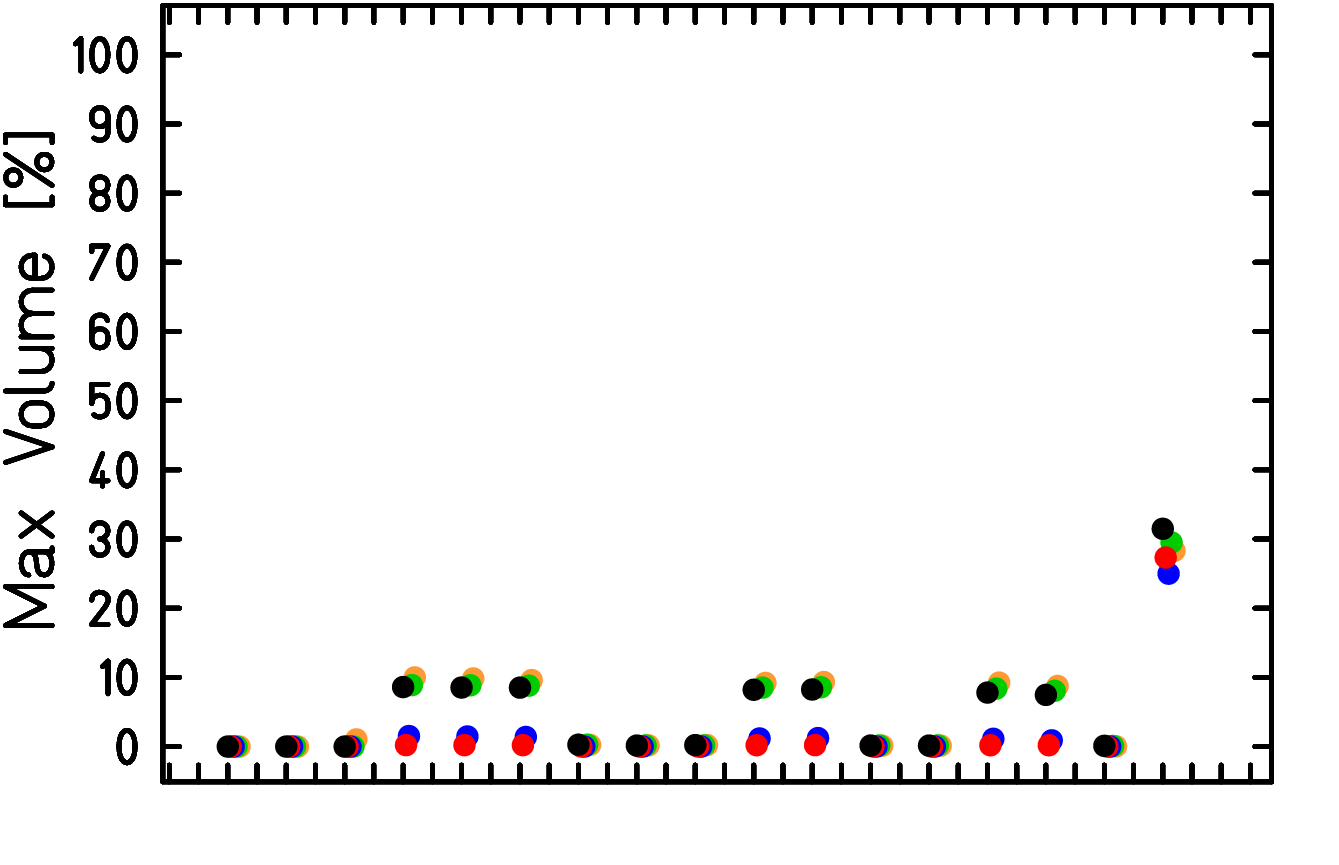
\includegraphics[width=\textwidth]{Mayo_Human_BeamDirection_RV_MaxVolume.png}
\end{minipage}

\hfill

\begin{minipage}{0.31\textwidth}
    \begin{overpic}
    [width=\textwidth]{Mayo_Human_BeamDirection_LCA_MeanDose.png}
    \put(40,80){LCA}
    \end{overpic} 
\end{minipage}
\hfill
\begin{minipage}{0.31\textwidth}
  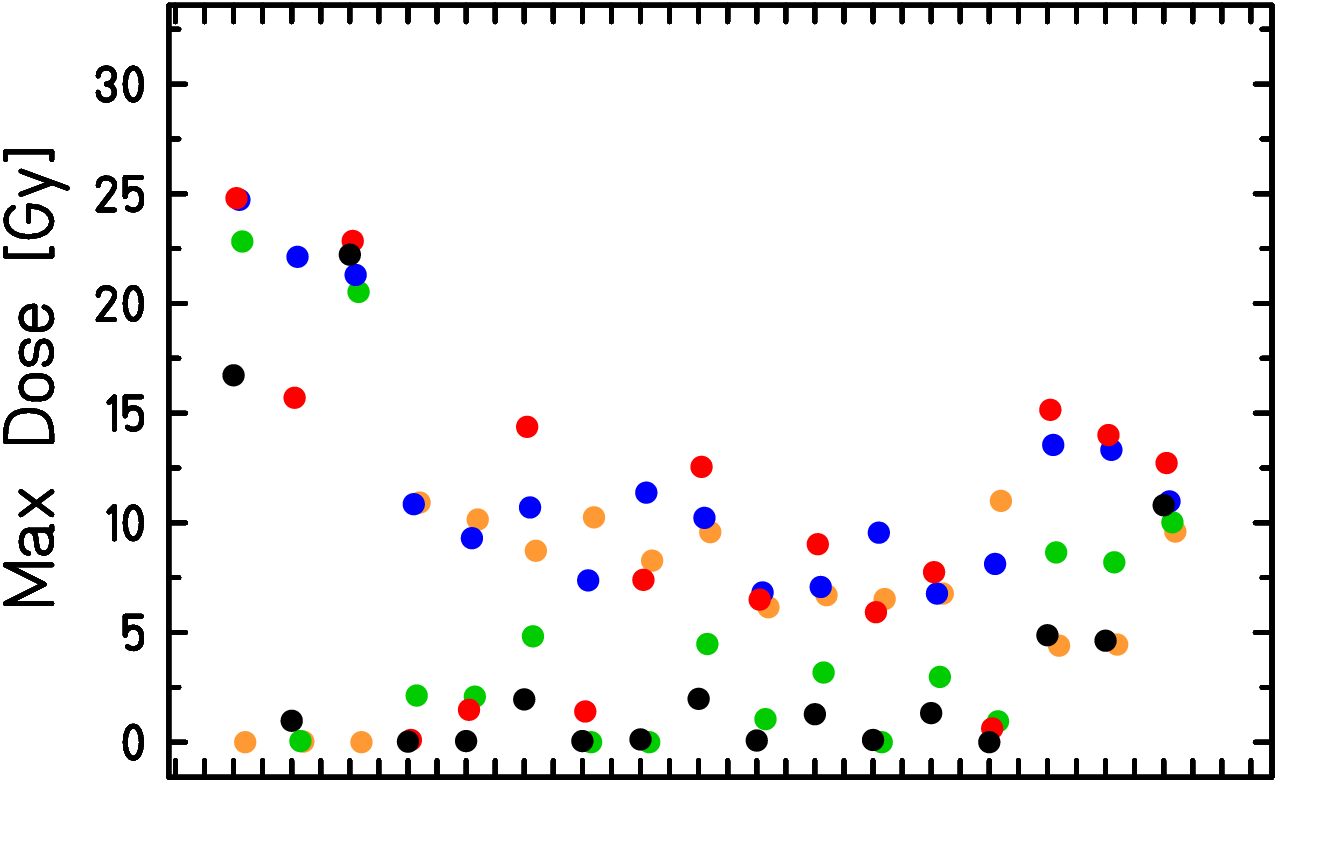
\includegraphics[width=\textwidth]{Mayo_Human_BeamDirection_LCA_MaxDose.png}
\end{minipage}
\hfill
\begin{minipage}{0.31\textwidth}
  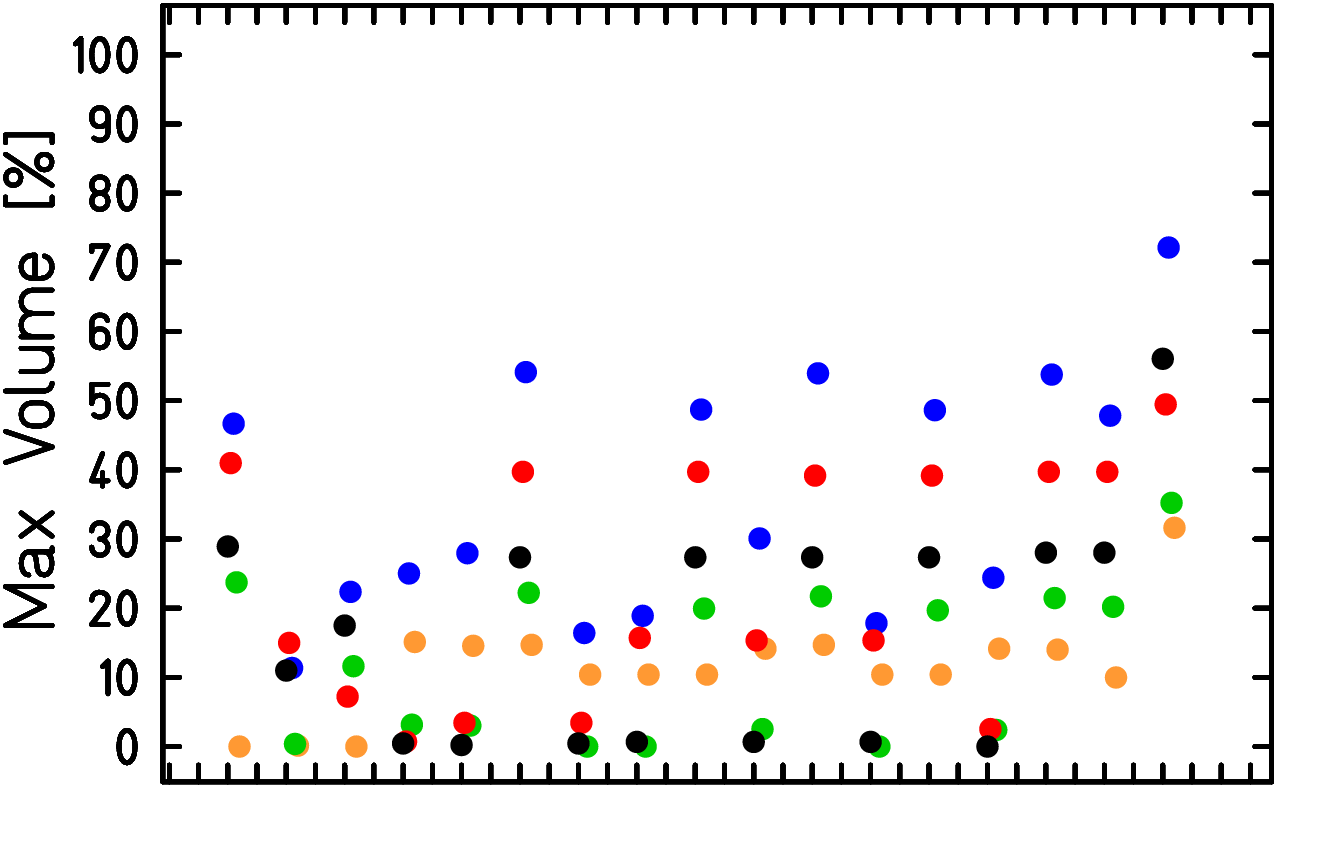
\includegraphics[width=\textwidth]{Mayo_Human_BeamDirection_LCA_MaxVolume.png}
\end{minipage}


\hfill

\begin{minipage}{0.31\textwidth}
    \begin{overpic}
    [width=\textwidth]{Mayo_Human_BeamDirection_RCA_MeanDose.png}
    \put(40,120){RCA}
    \end{overpic} 
\end{minipage}
\hfill
\begin{minipage}{0.31\textwidth}
  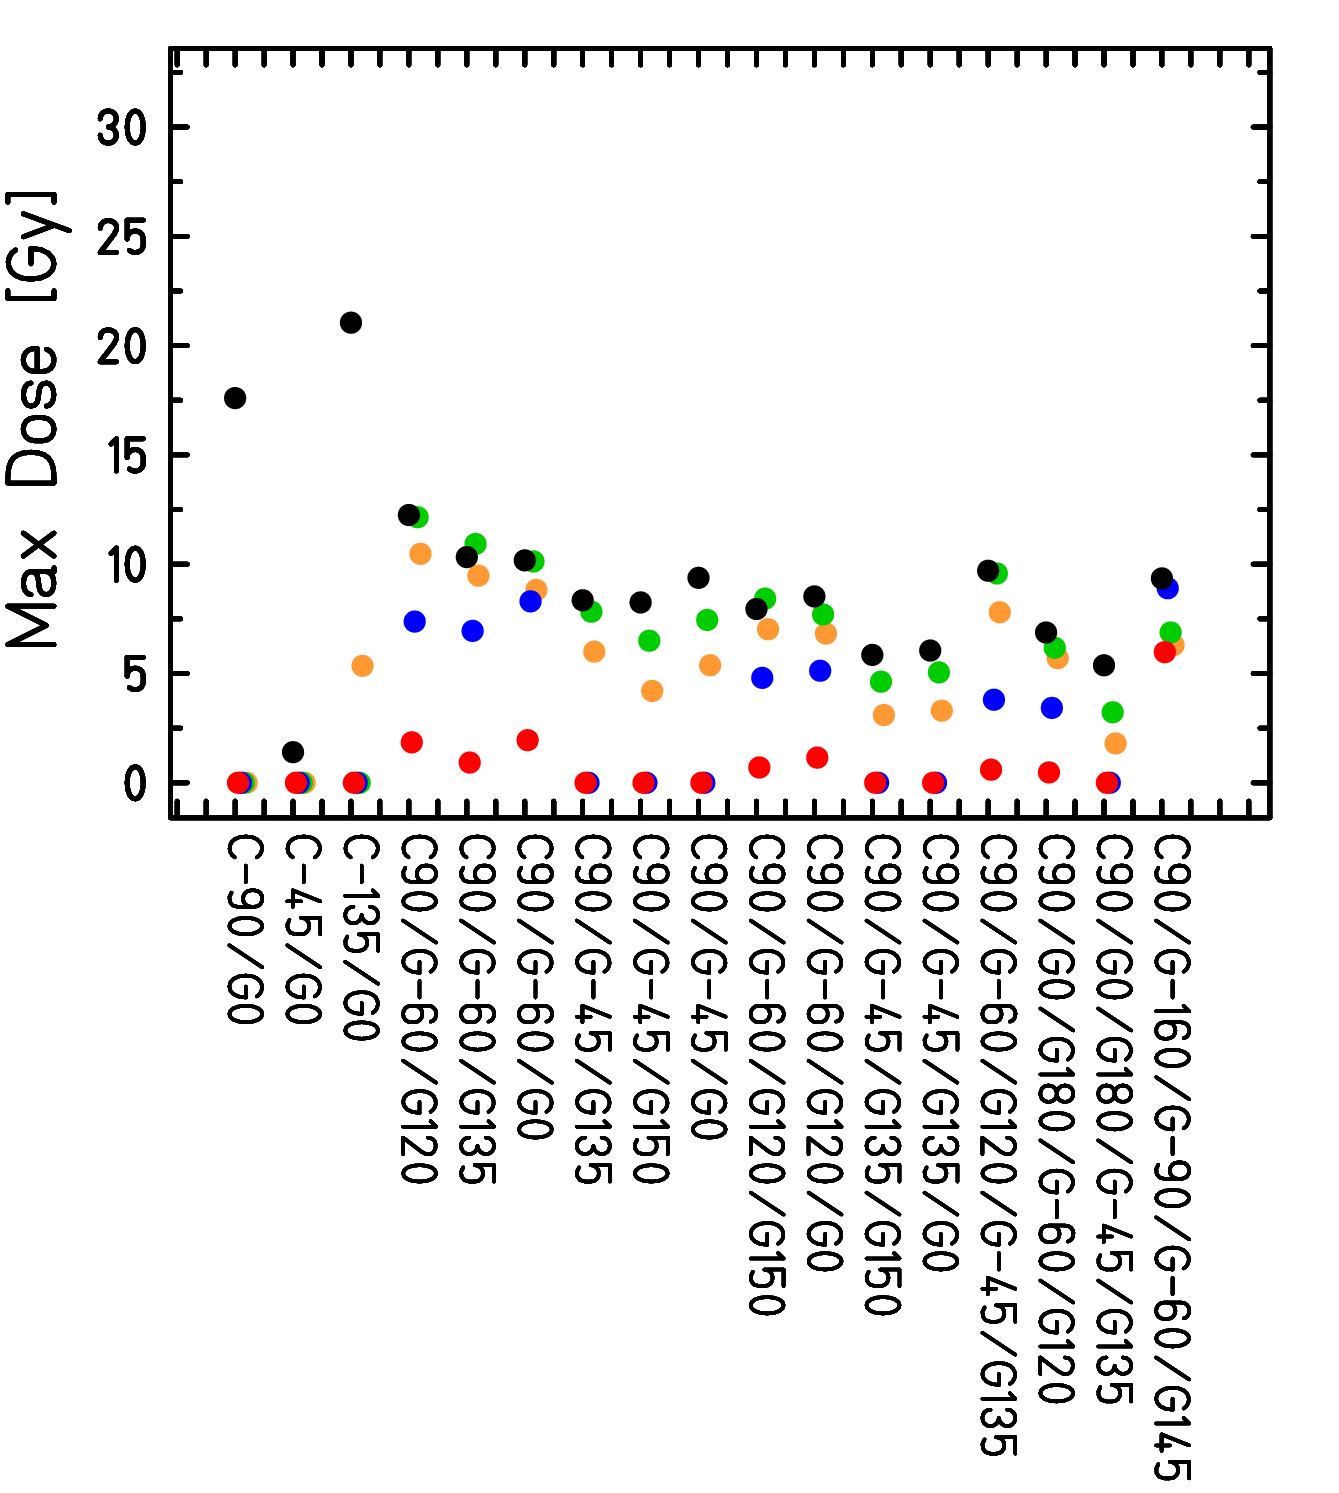
\includegraphics[width=\textwidth]{Mayo_Human_BeamDirection_RCA_MaxDose.png}
\end{minipage}
\hfill
\begin{minipage}{0.31\textwidth}
  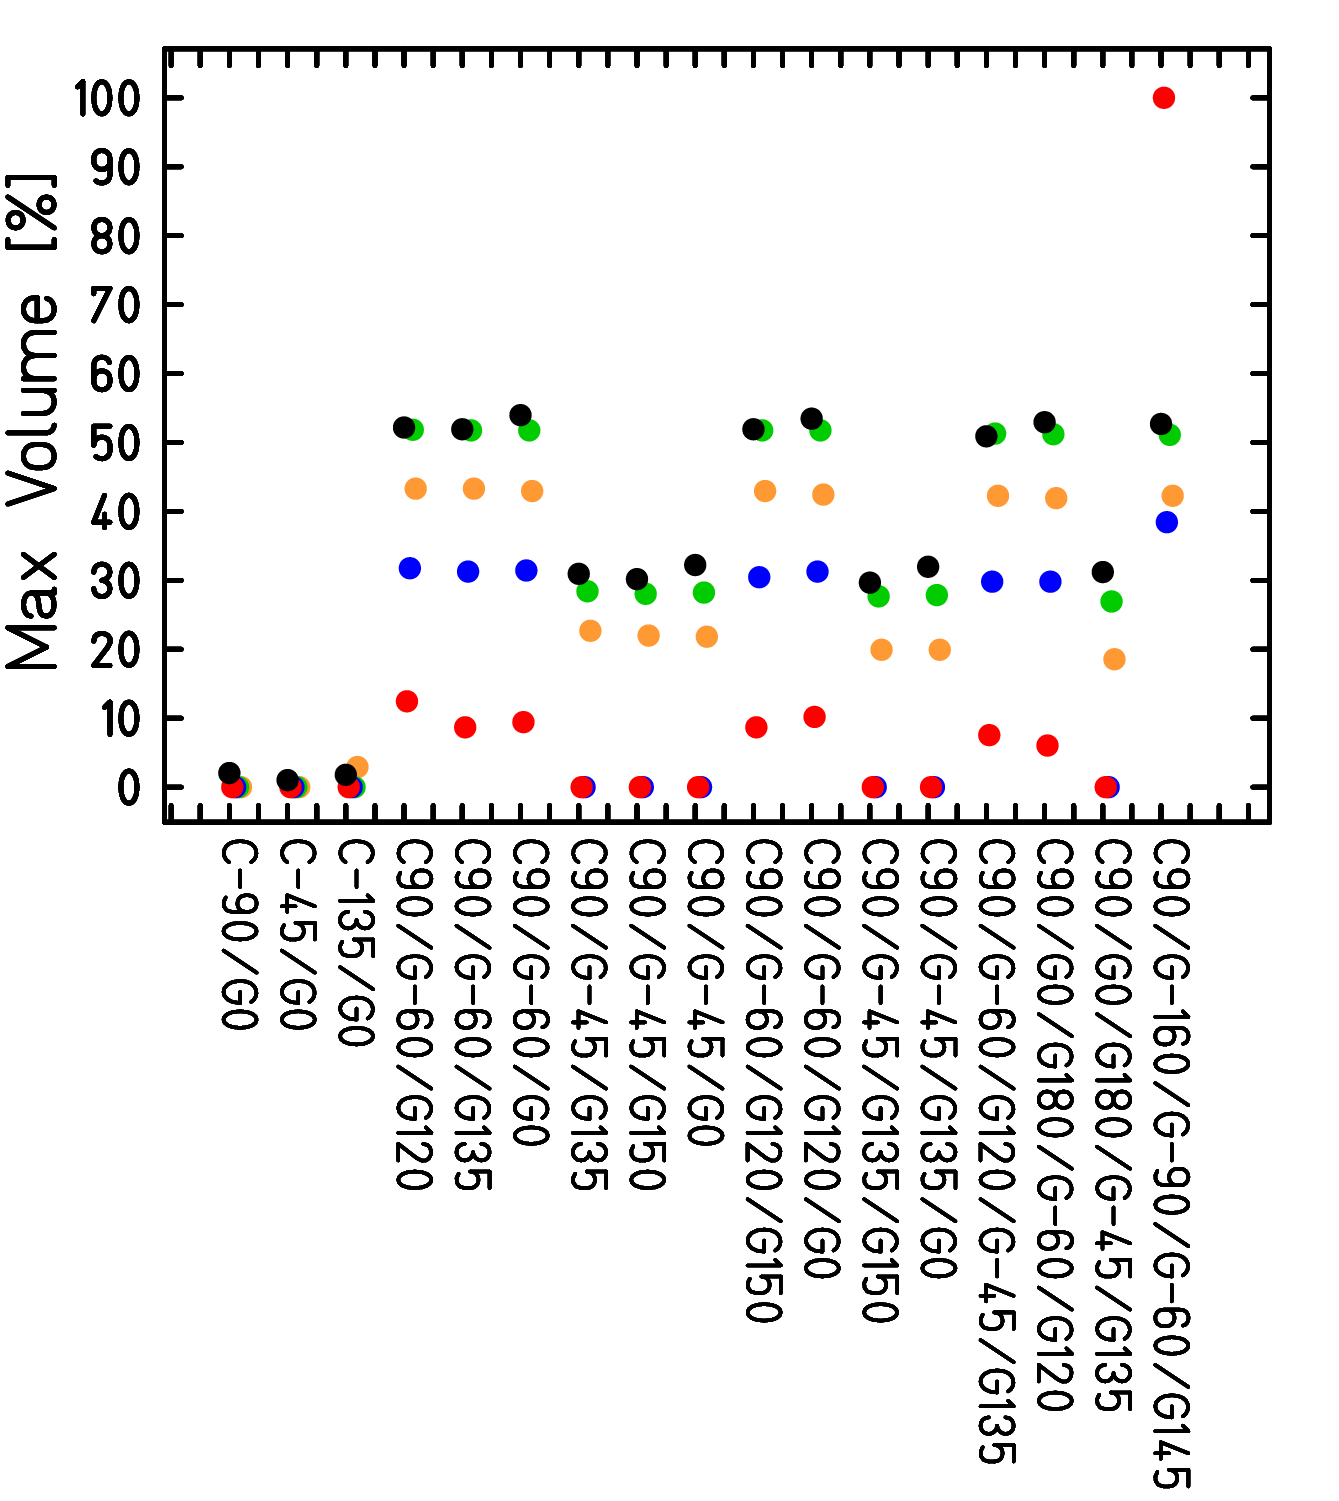
\includegraphics[width=\textwidth]{Mayo_Human_BeamDirection_RCA_MaxVolume.png}
\end{minipage}

  \caption{Mean and maximum dose as well as maximal irradiated volume of the heart (first row) as well as cardiac substructures (second row: 
  LV, third row: RV, fourth row: LCA, last row: RCA) when irradiating the LPV and RPV in the five patient data sets with different field 
  numbers and beam directions. The different patients are displayed in different colors (patient 1: black, 2: red, 3: blue, 4: green, 5: 
  orange). The different beam channel directions are stated in the the figures of the last row.}
  \label{beamdirection_MeanMaxD_MaxV}
  
\end{figure}

\newpage

\subsection{Safety margin limitations}
\label{safetymarginlimitation}

Figure \ref{margin_boxplot} shows the dose results for the main OARs when irradiating the PVs with no safety margin (0mm) and different additional, 
isotropic safety margins (3mm, 5mm or 7mm). The dose-volume-limits were studied according to the recommendation of RTOG (see table \ref{tab:RTOG}) 
and the limit for each organ is indicated by a dashed line in the boxplots. Besides an IMPT treatment IMPT(OAR) deliveries were also 
studied. Thereby the esophagus was implemented as a critical structure in the optimization process with two different restrictions 
(IMPT(OAR)$_{R1}$ and (IMPT(OAR)$_{R2}$). In IMPT(OAR)$_{R1}$ it was stated that this structure should not receive more than 70\% of the 
physical dose of 25Gy, while IMPT(OAR)$_{R2}$ had stronger restrictions with the maximal dose deposition set to 30\% of the physical dose. 
The results of these three treatment deliveries are shown in each column of the plot.\newline
\newline
As expected, the dose to the enclosed OAR increases with increasing safety margin for all patients. This is the case both for IMPT and IMPT(OAR) 
deliveries. Nevertheless the IMPT(OAR) deliveries lead to a reduced dose deposition, especially in the esophagus. For no safety margin, 
the median dose to the esophagus over all patients is found to be 8.5Gy (75th percentile: 12.4Gy), which decreases to 7.0Gy (9.0Gy) with IMPT(OAR)$_{R1}$ delivery and 
to 2.8Gy (4.4Gy) with IMPT(OAR)$_{R2}$. For 3mm safety margin and ab IMPT irradiation resulted in 13.0Gy (18.6Gy) and reduces to 9.3Gy (12.1Gy) 
for IMPT(OAR)$_{R1}$ and 3.5Gy (6.0Gy) for IMPT(OAR)$_{R2}$. With 5mm safety margin the RTOG limit of 11.9Gy starts to be exceeded for  
IMPT(OAR)$_{R1}$ deliveries as it was found to be 11.8Gy (15.1Gy) (compared to 19.0Gy (22.8Gy) with IMPT). With the stronger restrictions on 
the other hand the dose to the esophagus remains under the stated limit with 4.3Gy(6.6Gy). Even for a margin of 7mm the 
stronger restrictions result in an appropiate dose deposition with a median of 6.0Gy (7.9Gy). 
For IMPT(OAR)$_{R1}$ the 7mm margin result increased further to 14.3Gy (17.1Gy) (IMPT irradiation: 23.3Gy (24.6Gy)).\newline
\newline
Even though only the esophagus is included in the IMPT optimization process, also other OAR profit from this irradiation mode. This can be 
understood as the beam stopping in front of the esophagus (gantry angle of -45$^{\circ}$) is optimized into having less raster points in the 
IMPT(OAR) delivery compared to an IMPT irradiation and hence a reduced dose contribution to the total dose delivery. The other beam 
channels (gantry angles of 135$^{\circ}$ and 0$^{\circ}$) are hence optimized into having more raster points compared to the IMPT delivery, 
contributing more to the dose deposition. Adjacent OAR to the esophagus, like trachea and aorta, are thus also receiving a smaller dose 
deposition from the beam channel stopping in proximity to them. As only an IMPT(OAR) treatment leads to acceptable dose depositions in the esophagus, 
the median dose to the other organs will only be stated for this delivery type.\newline
\newline
Over all patients the trachea is receiving a median dose of 
0Gy in all cases, since only patient 2 and 3 yield a dose in this critical structure. The 75th percentile is found to be 0.1Gy with no 
safety margin and 1.1Gy, 3.0Gy, 6.6Gy for 3mm, 5mm and 7mm, respectively for IMPT(OAR)$_{R1}$. For IMPT(OAR)$_{R2}$ the 75th percentile 
results also to 0.1Gy for no safety margin and 0.5Gy, 3.0Gy, 7.4Gy for 3mm, 5mm and 7mm, respectively. 
All of these dose deposition are far below the recommended dose-volume-limit for the trachea (10.5Gy for 4cm$^{3}$).\newline
\newline
For the aorta an IMPT(OAR)$_{R1}$ irradiation with no safety margin leads to a median dose deposition of 6.5Gy (8.5Gy), while 8.3Gy 
(10.6Gy), 9.8Gy (12.3Gy) and 11.3Gy (14.0Gy) are deposited with 3mm, 5mm and 7mm margin. In case of IMPT(OAR)$_{R2}$ these results are 
further reduced to 3.5Gy (5.3Gy) with no safety margin and 5.0Gy (7.9Gy), 6.3Gy (12.0Gy) and 7.8Gy (13.6Gy) with 3mm, 5mm and 7mm margin, respectively. 
Also these results are far below the critical dose-volume limit of 31Gy for 10cm$^{3}$. It can thus be concluded that trachea and aorta do 
not receive a critical dose deposition while treating the PVs with a dose of 25Gy.\newline 
\newline
For the heart the dose-volume limits are much more critical. A median of 18.3Gy (22.8Gy) was obtained for IMPT(OAR)$_{R1}$ irradiations with 
no safety margin and 23.0Gy (24.9Gy), 24.3Gy (25.0Gy) and 24.8Gy (25.0Gy) for 3mm, 5mm and 7mm margin, respectively. These results are 
slightly decreased with IMPT(OAR)$_{R2}$ where the median is found to be 16.5Gy (21.0Gy) for no margin and 20.0Gy (24.0Gy), 22.0Gy (25.3Gy) 
and 22.8Gy (17.8Gy) for 3mm, 5mm and 7mm margin, respectively. 
Hence all studied irradiations by far exceed the dose-volume limit of 16Gy for 15cm$^{3}$. 
A close analysis of the radiosensitive cardiac substructures is presented on the next pages (in table \ref{tab:meandose_heart} to table 
\ref{tab:maxvolume_ca}). 

%%%%%%%%%%%%%%%%%%%%%%%%
%%%%%%%% DOSE TO OAR %%%
%%%%%%%%%%%%%%%%%%%%%%%%

\newpage

\begin{figure}[H]

\hfill
\begin{minipage}{0.3\textwidth}
\hspace*{1.6cm} IMPT 
\end{minipage}
\hfill
\begin{minipage}{0.3\textwidth}
 \hspace*{1.3cm} IMPT(OAR)$_{R1}$ 
\end{minipage}
\hfill
\begin{minipage}{0.3\textwidth}
\hspace*{1.3cm} IMPT(OAR)$_{R2}$ 
\end{minipage}
\hfill

\vspace*{0.3cm}

\begin{minipage}{0.31\textwidth}
  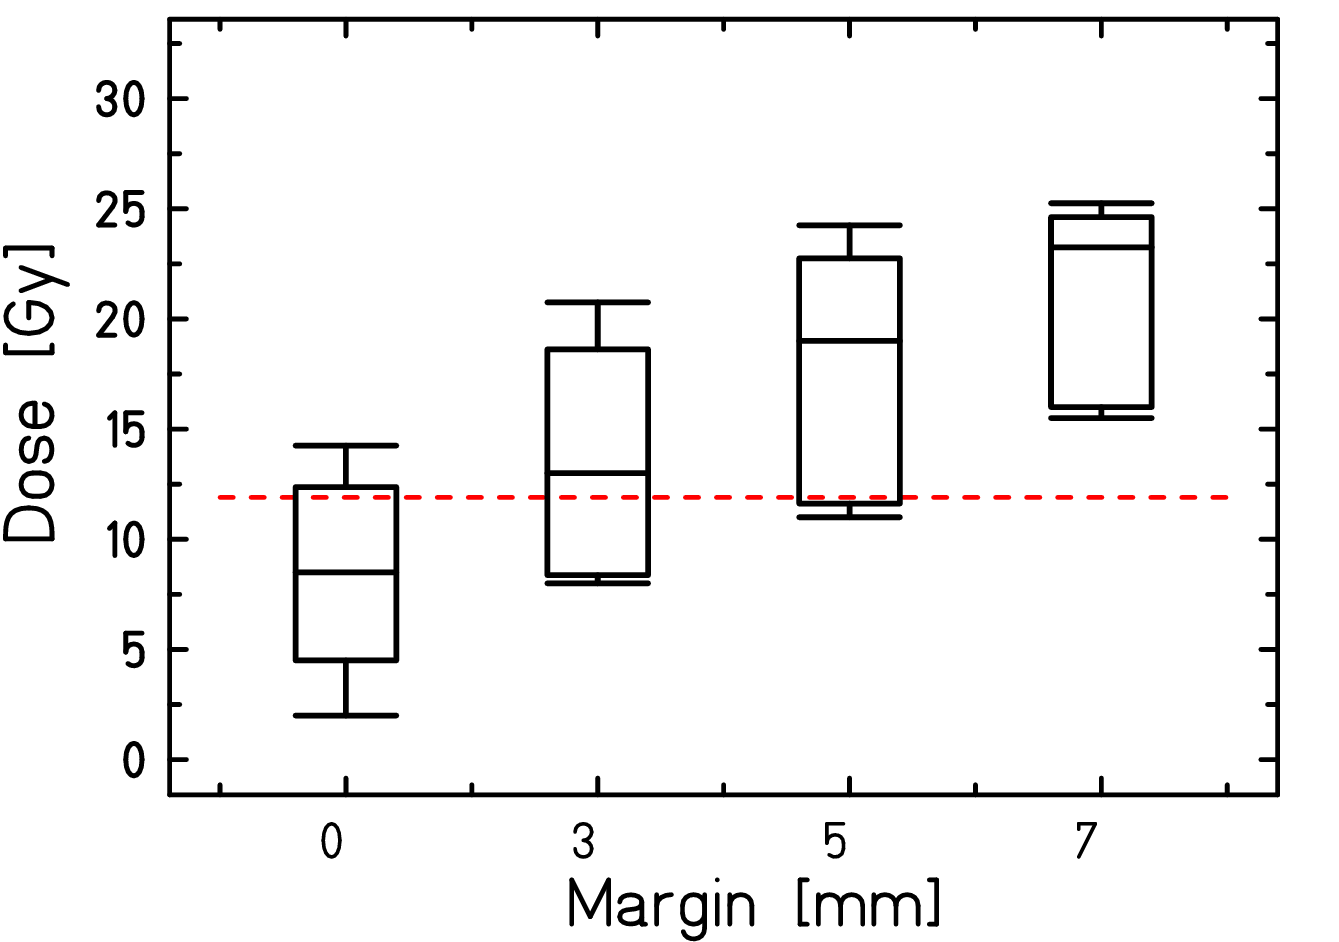
\includegraphics[width=\textwidth]{Whisker_ESO_alternativeLimit_ITV.png}
\end{minipage}
\hfill
\begin{minipage}{0.31\textwidth}
  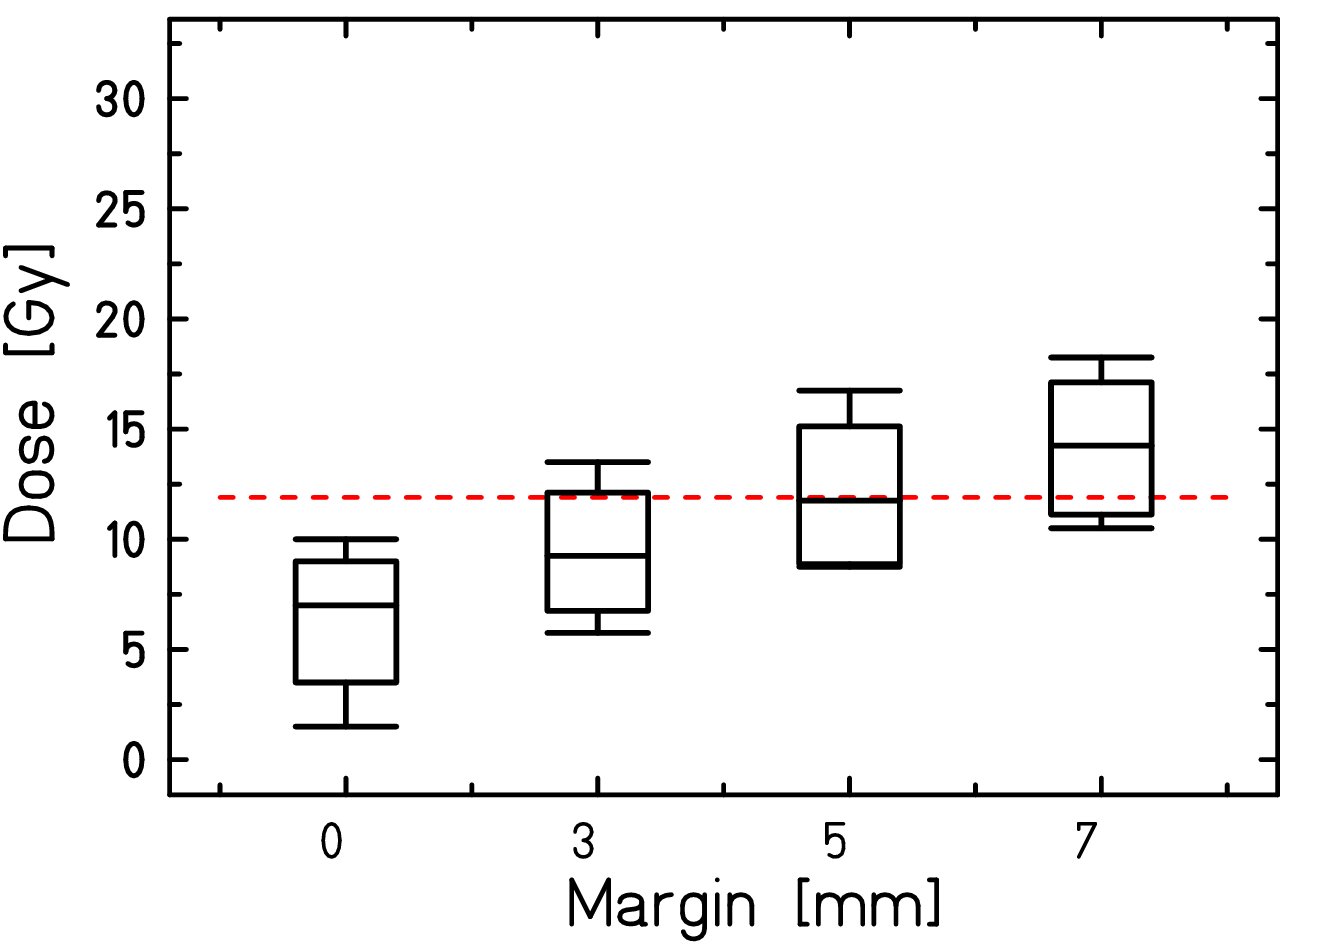
\includegraphics[width=\textwidth]{Whisker_ESO_alternativeLimit_IMPT_woOverlap.png}
\end{minipage}
\hfill
\begin{minipage}{0.31\textwidth}
  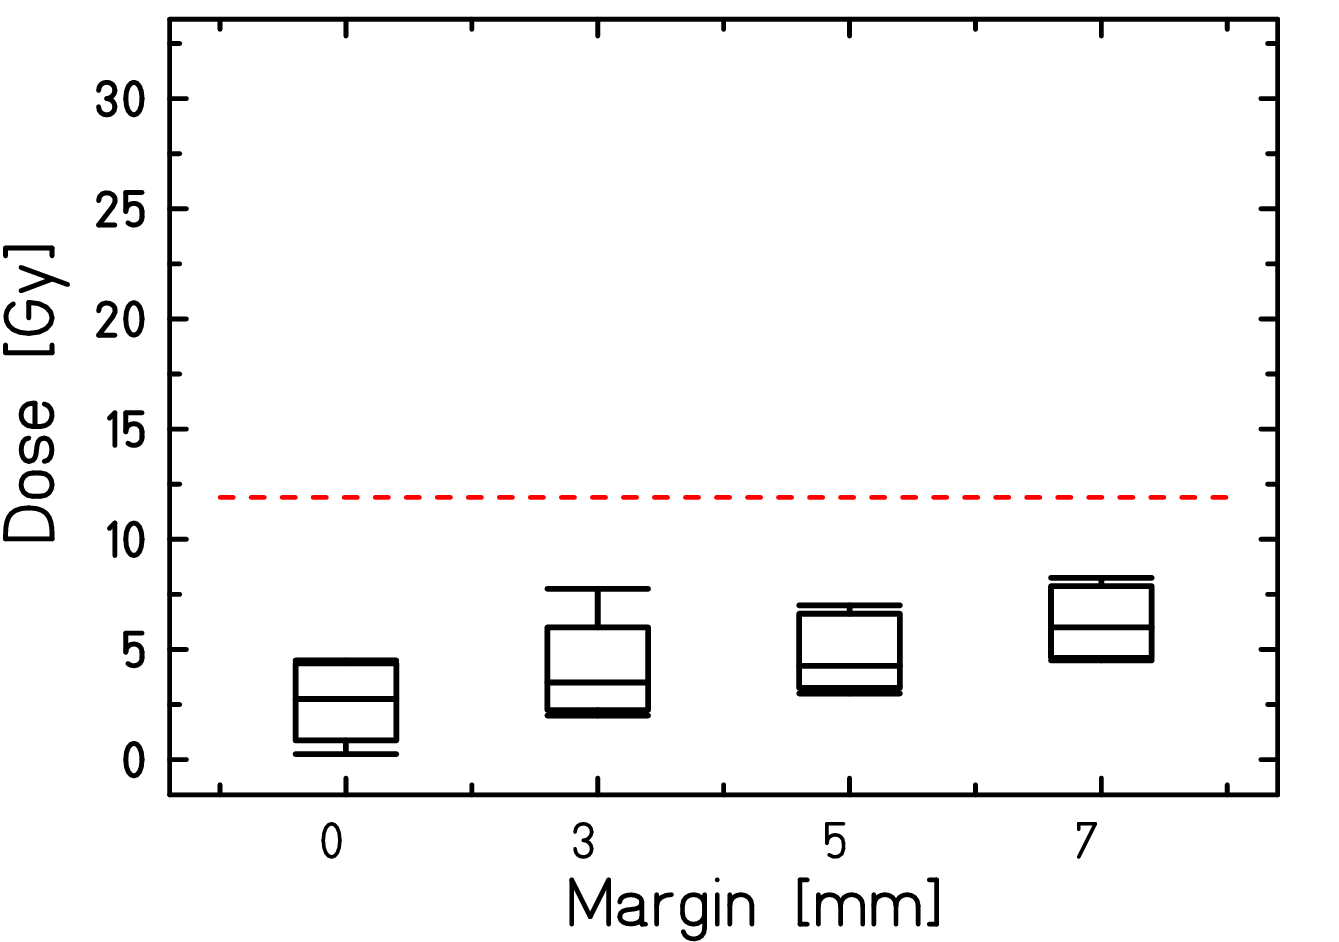
\includegraphics[width=\textwidth]{Whisker_ESO_alternativeLimit_IMPT_woOverlap_otherParameters.png}
\end{minipage}
\hfill
\vspace*{0.1cm}
\begin{minipage}{\textwidth}
 \hspace*{7.5cm} (a) Esophagus \\
\end{minipage}
\hfill
\begin{minipage}{0.31\textwidth}
  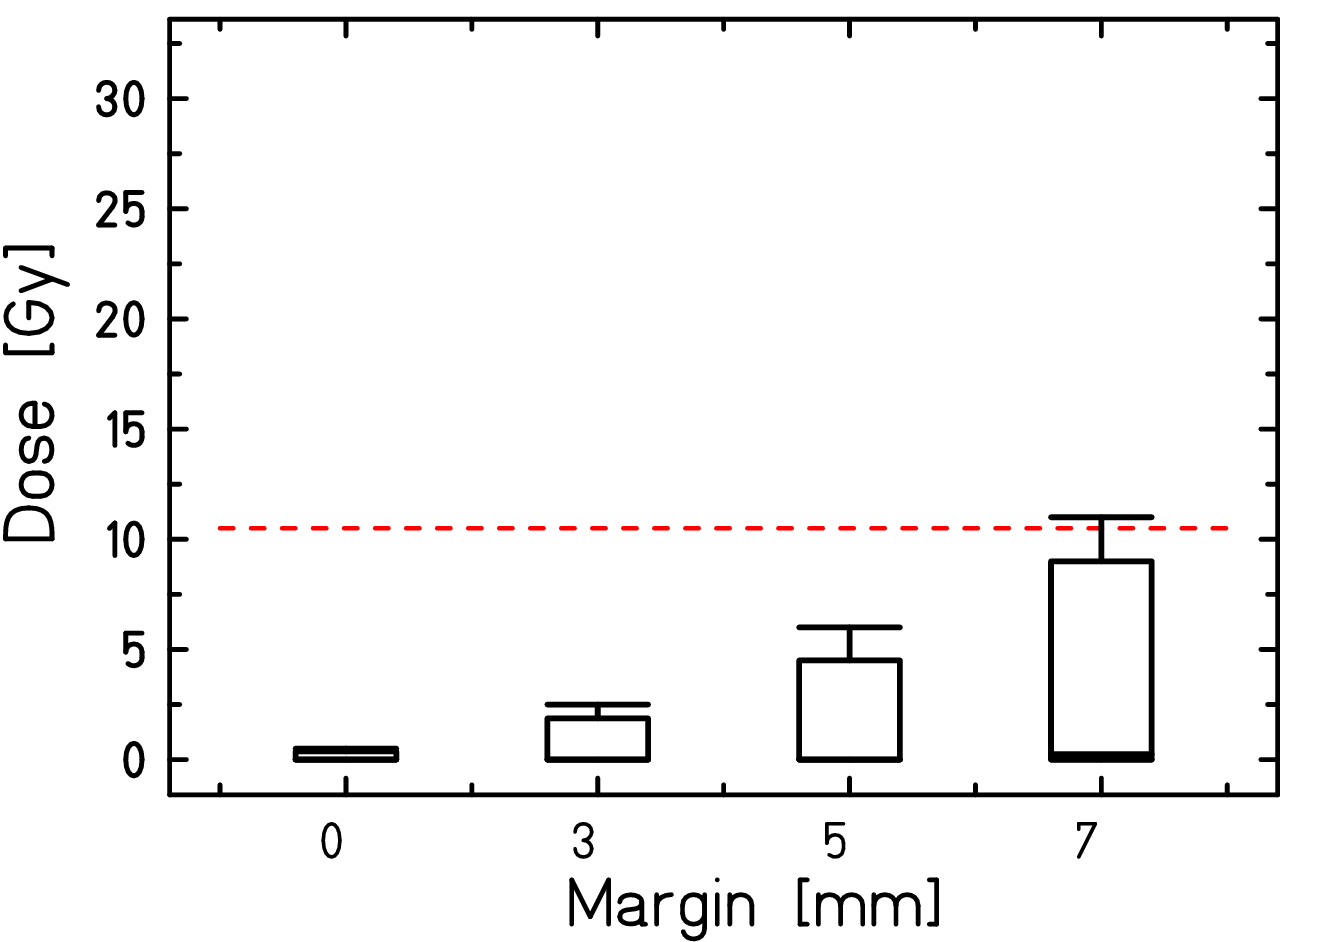
\includegraphics[width=\textwidth]{Whisker_TRACHEA_ITV.png}
\end{minipage}
\hfill
\begin{minipage}{0.31\textwidth}
  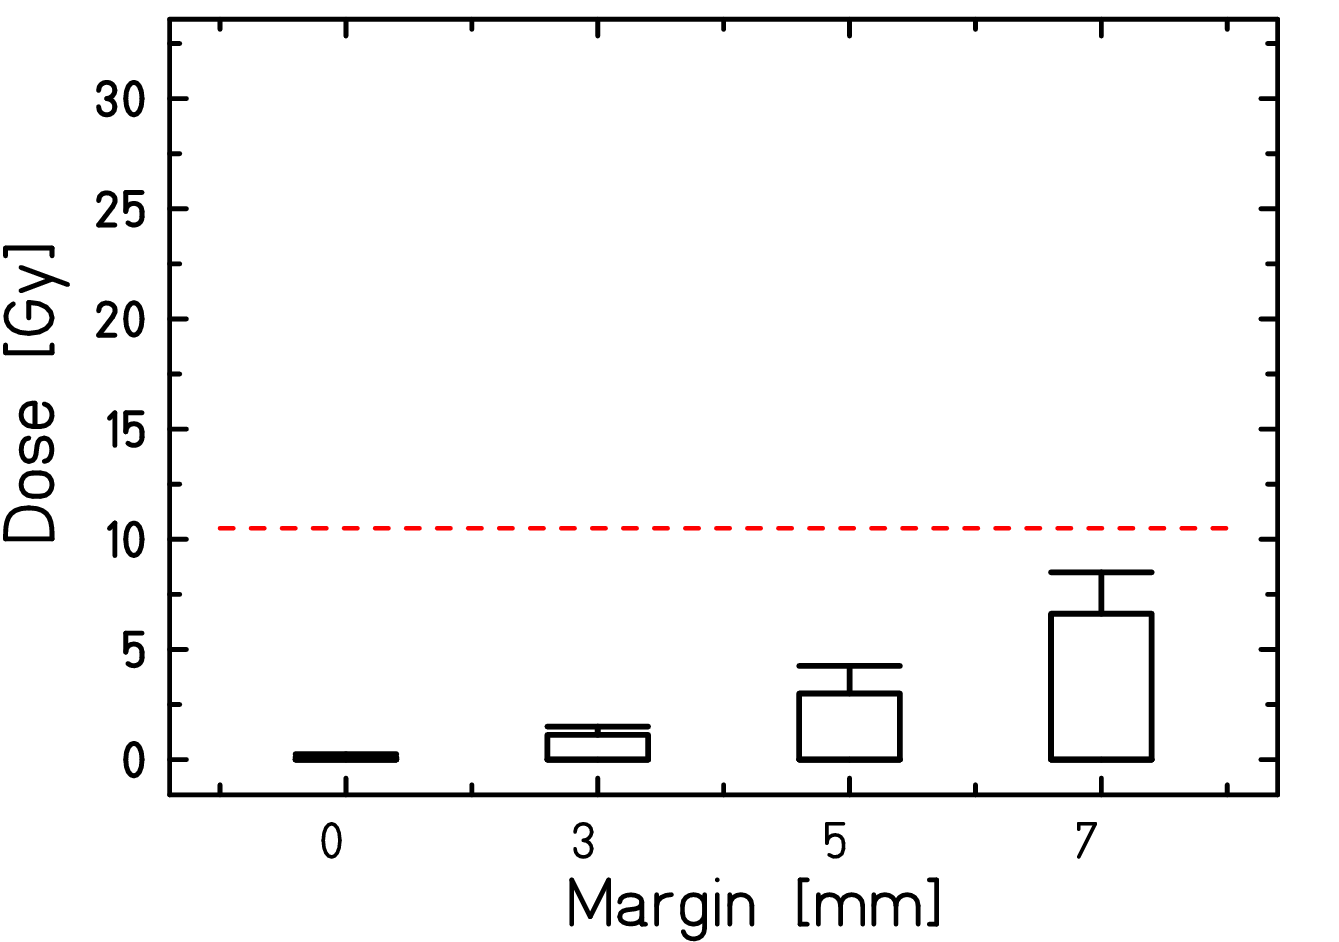
\includegraphics[width=\textwidth]{Whisker_TRACHEA_IMPT_woOverlap.png}
\end{minipage}
\hfill
\begin{minipage}{0.31\textwidth}
  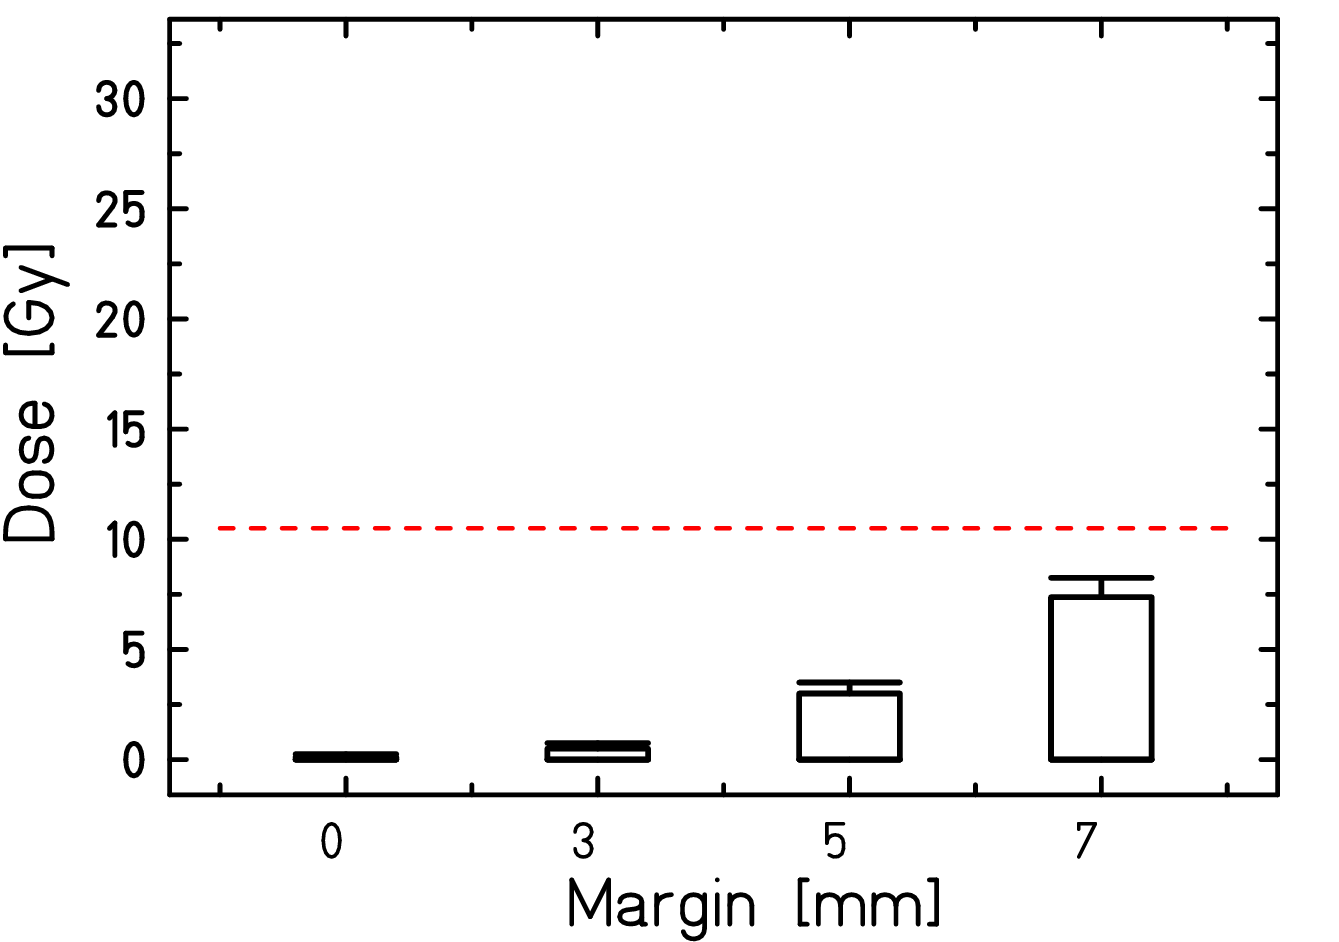
\includegraphics[width=\textwidth]{Whisker_TRACHEA_IMPT_woOverlap_otherParameters.png}
\end{minipage}
\hfill
\vspace*{0.1cm}
\begin{minipage}{\textwidth}
 \hspace*{7.5cm} (b) Trachea \\
\end{minipage}
\hfill
\begin{minipage}{0.31\textwidth}
  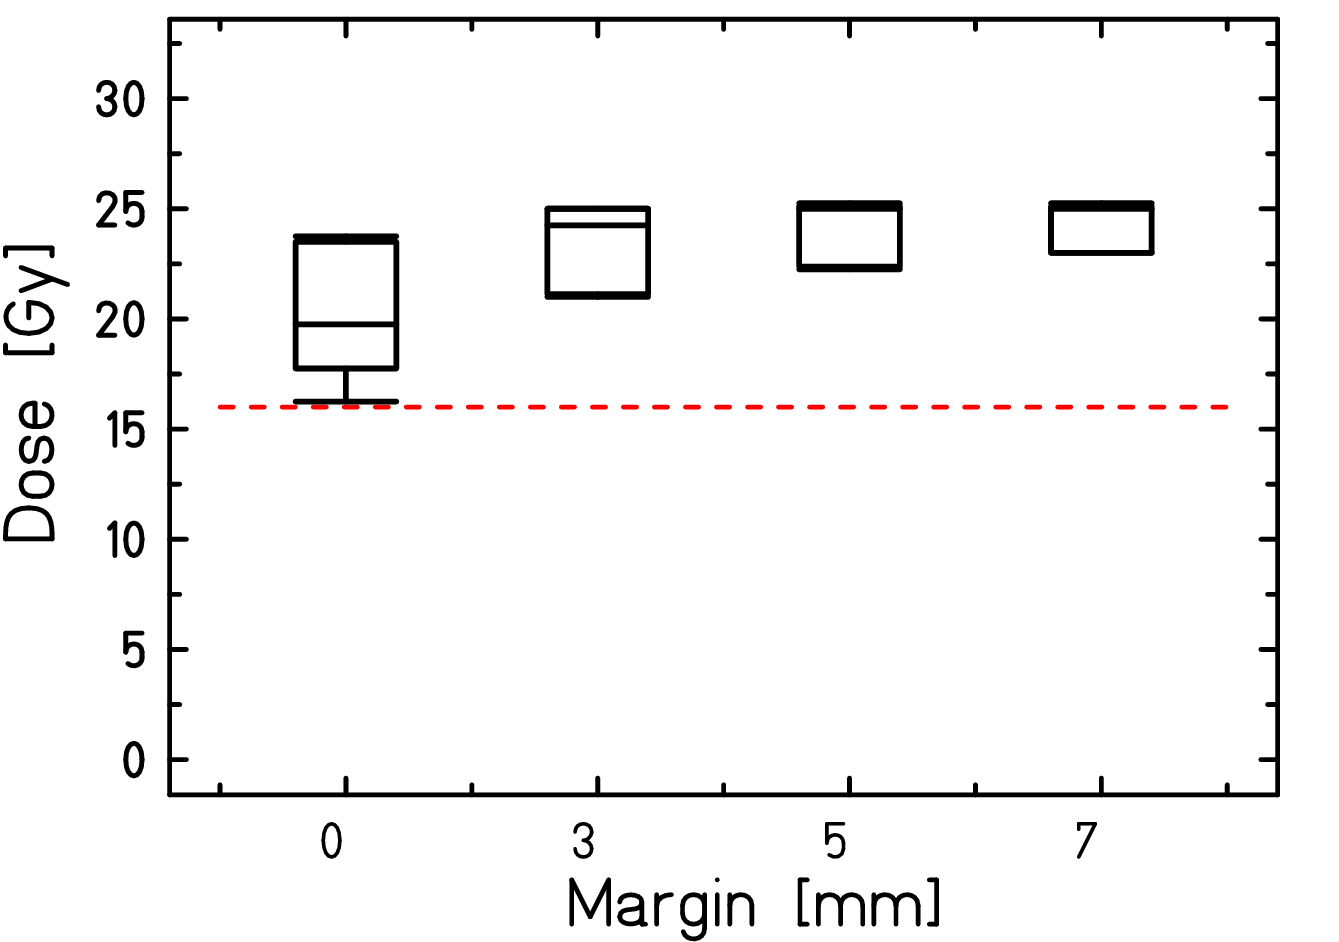
\includegraphics[width=\textwidth]{Whisker_HEARTwoOverlap_ITV.png}
\end{minipage}
\hfill
\begin{minipage}{0.31\textwidth}
  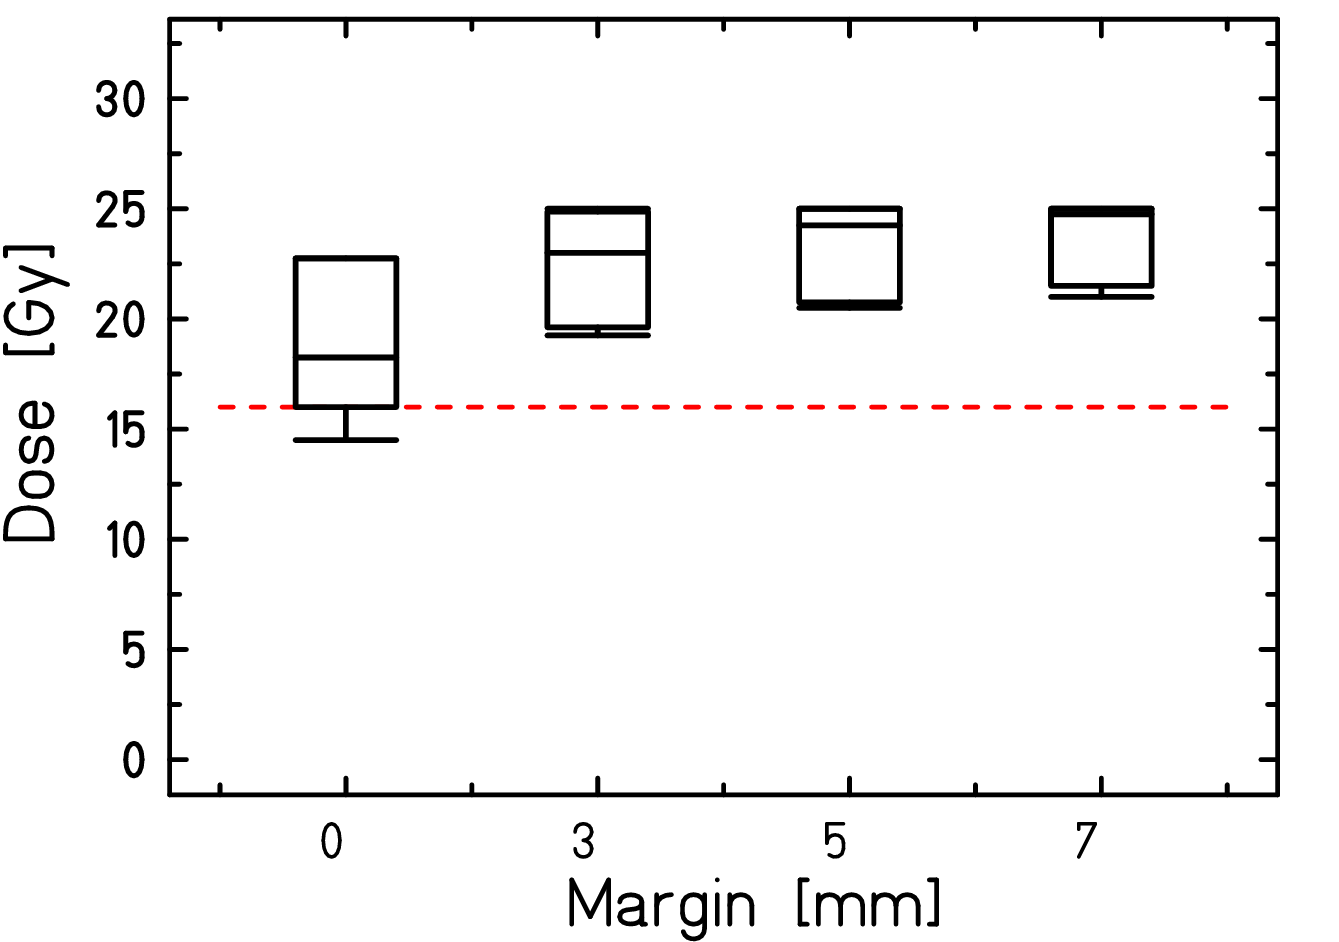
\includegraphics[width=\textwidth]{Whisker_HEARTwoOverlap_IMPT_woOverlap.png}
\end{minipage}
\hfill
\begin{minipage}{0.31\textwidth}
  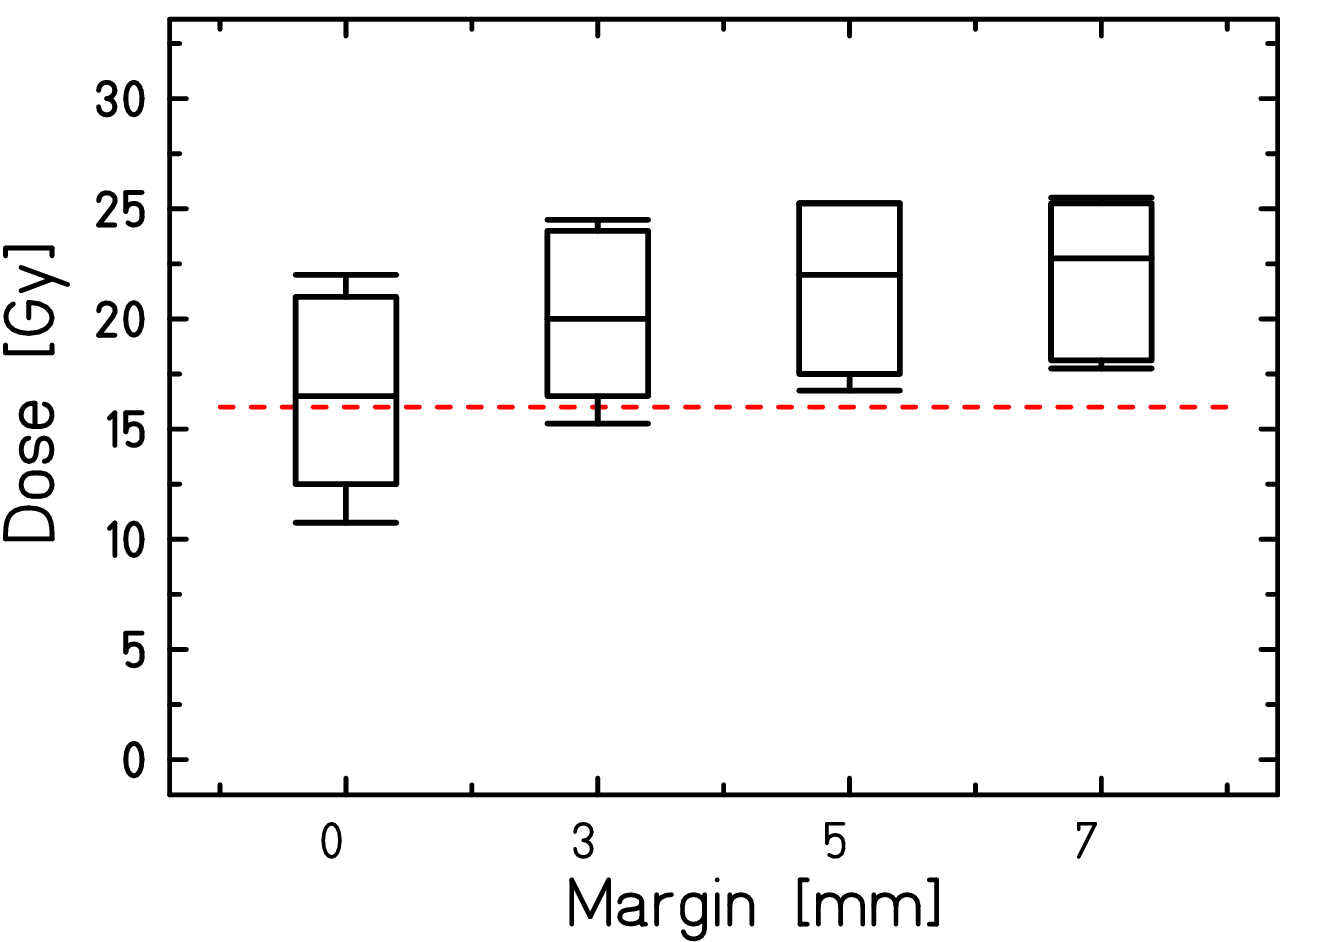
\includegraphics[width=\textwidth]{Whisker_HEARTwoOverlap_IMPT_woOverlap_otherParameters.png}
\end{minipage}
\hfill
\vspace*{0.1cm}
\begin{minipage}{\textwidth}
 \hspace*{7.5cm} (c) Heart \\
\end{minipage}
\hfill
\begin{minipage}{0.31\textwidth}
  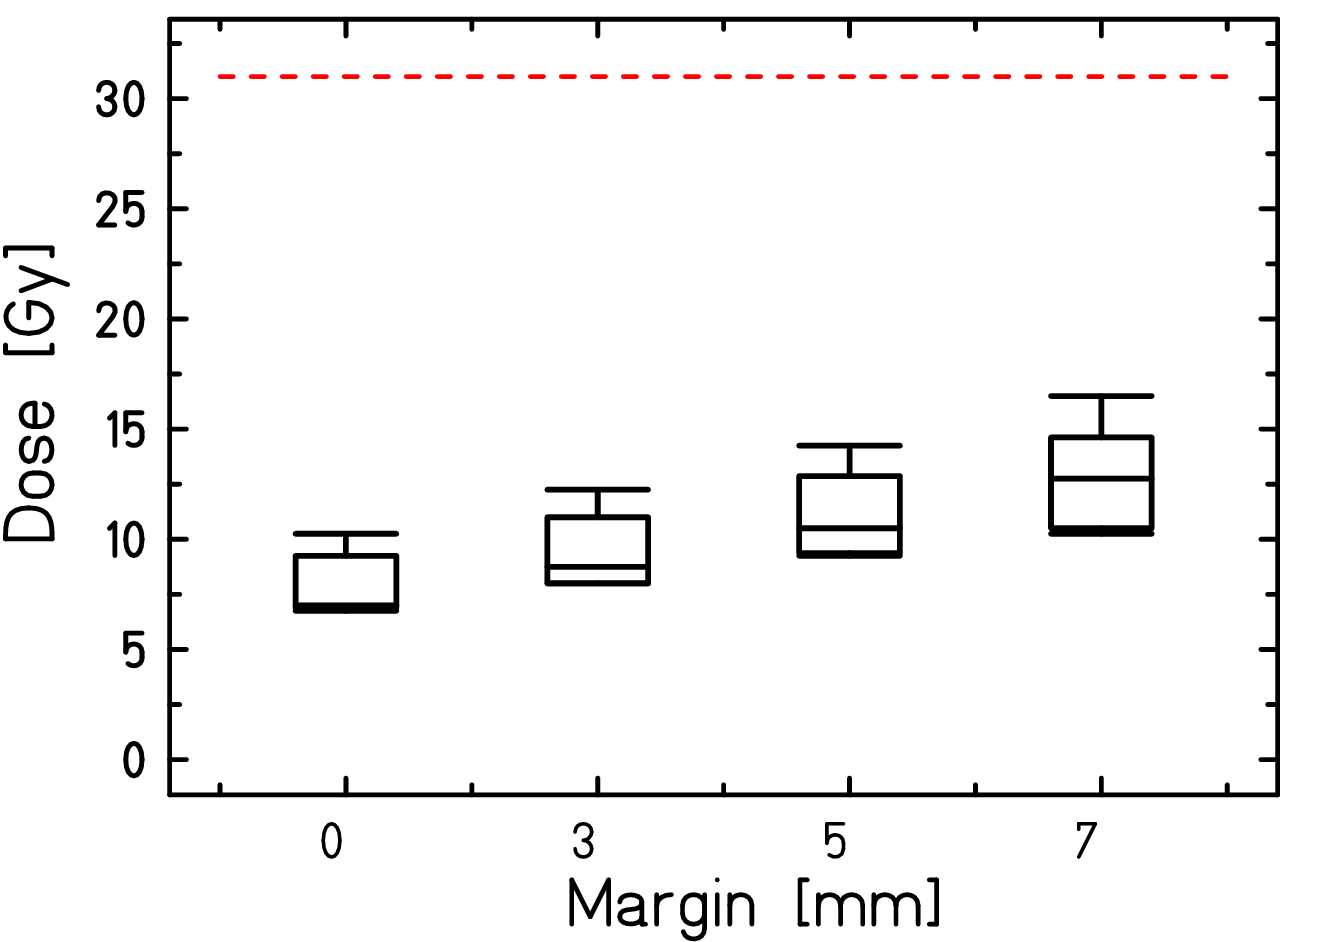
\includegraphics[width=\textwidth]{Whisker_AORTA_ITV.png}
\end{minipage}
\hfill
\begin{minipage}{0.31\textwidth}
\hspace*{-0.35cm}
 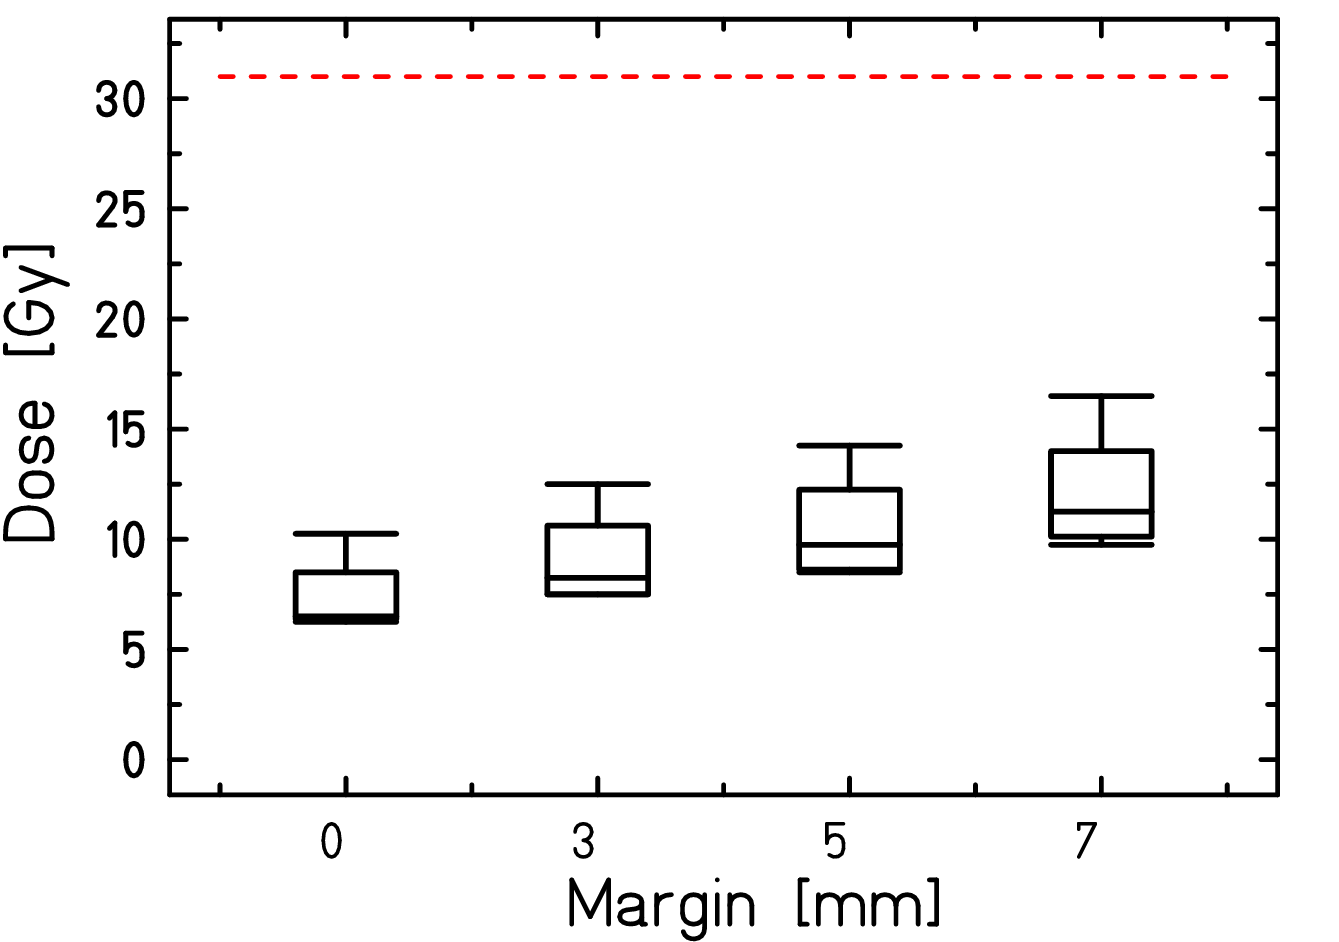
\includegraphics[width=\textwidth]{Whisker_AORTA_IMPT_woOverlap.png}
\end{minipage}
\hfill
\begin{minipage}{0.31\textwidth}
\hspace*{-0.5cm}
 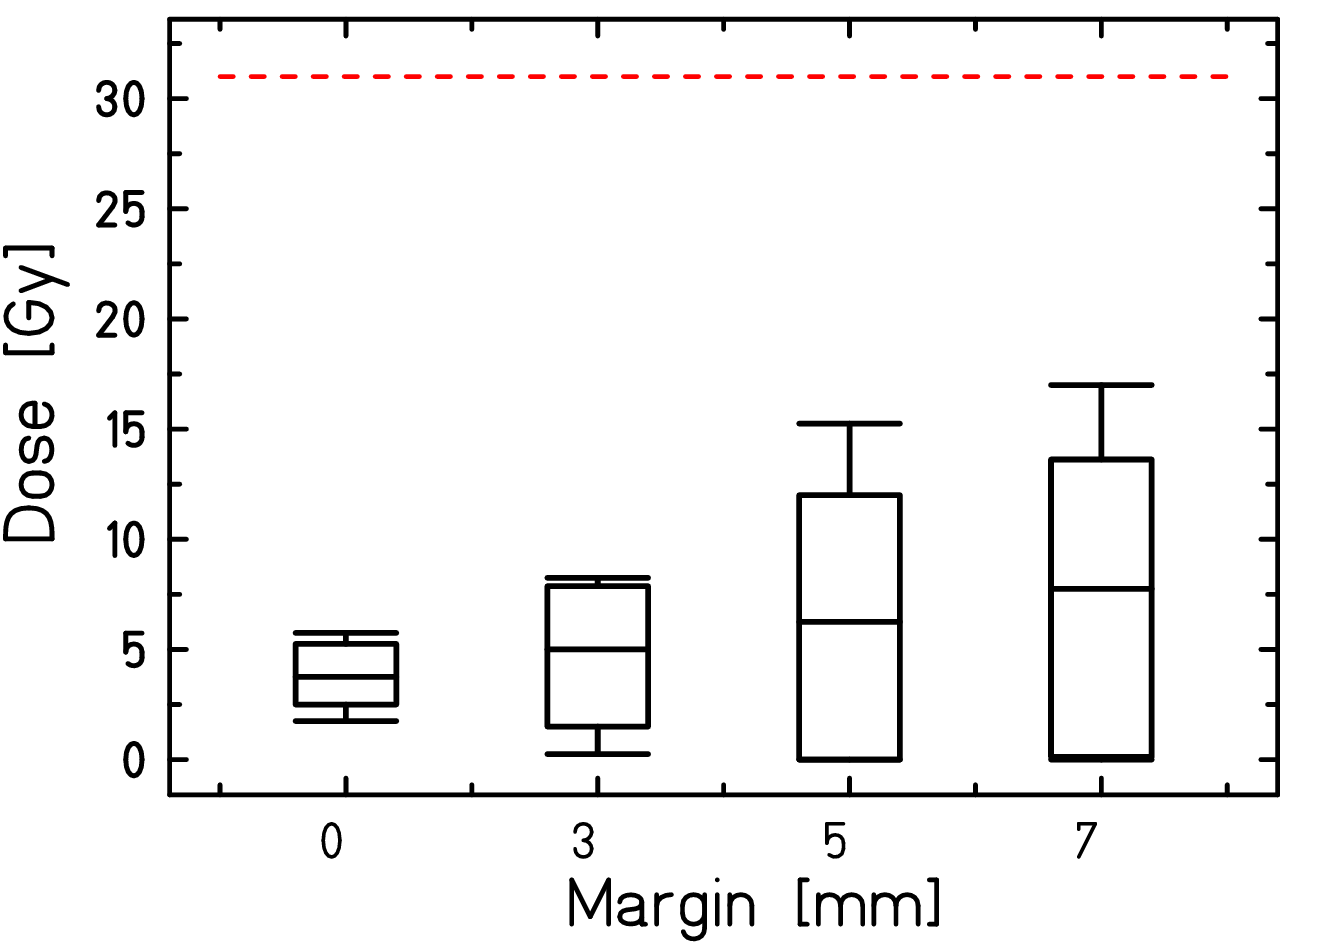
\includegraphics[width=\textwidth]{Whisker_AORTA_IMPT_woOverlap_otherParameters.png}
\end{minipage}
\hfill
\begin{minipage}{\textwidth}
 \hspace*{7.5cm} (d) Aorta \\
\end{minipage}
\caption{Boxplots of dose-volume data for different safety margins (0mm, 3mm, 5mm and 7mm) over all patients. 
The data is plotted for different OARs when irradiating the LPV and RPV as IMPT (first column) or IMPT(OAR) in the five patient data sets. 
The results for the different IMPT(OAR) restrictions are plotted individually, so that IMPT(OAR)$_{R1}$ (second column) are the treatment plans 
with a maximal dose of 70\% of the physical dose and a weightfactor of 75\% and IMPT(OAR)$_{R2}$ (third column) are the results for the treatment plans 
with a maximal dose of 30\% physical dose and a weightfactor of 200\%. The dose-volume-limit for each critical organ is indicated with a 
dashed line in each plot, respectively.}
\label{margin_boxplot}
  
\end{figure}

\newpage

%%%%%%%%%%%%%%%%%%%%%%%%%%%%
%%%% DOSE TO THE HEART %%%%%
%%%%%%%%%%%%%%%%%%%%%%%%%%%%
Closer analysis of the dose deposition in the heart was carried out. The result of the median and 75th percentile over all patients 
is shown in table \ref{tab:meandose_heart} for the mean dose and in table \ref{tab:maxdose_heart} for the maximal point dose.
The mean deposited dose in the heart is negligible and does not increase with the size of the safety margins. Furthermore no 
difference in between IMPT and IMPT(OAR)$_{R1}$ or IMPT(OAR)$_{R2}$ irradiation can be observed.  
While also the maximum point dose does not increase with added safety margin, it can be seen that IMPT(OAR) treatment does lead to a higher 
point dose compared to an IMPT irradiation. This is higher for the irradiation with stronger restrictions on the maximal dose to the 
esophagus.  


\vspace*{-0.3cm}

\begin{table}[H]
  \centering
  \footnotesize
  \caption{Mean dose to heart: median and 75th percentile.}
  \begin{tabular}{|c||c|c|c|}
    \hline\hline
      Margin & IMPT [Gy] & IMPT(OAR)$_{R1}$ [Gy] & IMPT(OAR)$_{R2}$ [Gy]\\
    \hline
    0 mm & 1.0 (1.3) & 1.0 (1.1) & 0.9 (0.9) \\
    3 mm & 1.3 (1.7) & 1.3 (1.5) & 1.1 (1.4) \\
    5 mm & 1.5 (1.9) & 1.4 (1.7) & 1.1 (1.4) \\
    7 mm & 1.6 (2.0) & 1.5 (1.8) & 1.1 (1.5) \\
    \hline\hline
  \end{tabular}
  \label{tab:meandose_heart}
\end{table}

\begin{table}[H]
  \centering
    \footnotesize
  \caption{Maximum point dose to heart: median and 75th percentile.}
  \begin{tabular}{|c||c|c|c|}
    \hline\hline
      Margin & IMPT [Gy] & IMPT(OAR)$_{R1}$ [Gy] & IMPT(OAR)$_{R2}$ [Gy]\\
    \hline
    0 mm & 26.9 (27.1) & 27.6 (29.6) & 34.1 (36.9) \\
    3 mm & 26.2 (27.3) & 28.4 (29.7) & 31.6 (36.4) \\
    5 mm & 26.5 (27.1) & 28.0 (29.1) & 30.7 (31.6) \\
    7 mm & 26.2 (28.0) & 26.8 (27.9) & 30.1 (31.0) \\
    \hline\hline
  \end{tabular}
  \label{tab:maxdose_heart}
\end{table}

This can be understood as the esophagus and the other adjacent 
OAR (trachea, aorta) receive in general less dose with IMPT(OAR) due to the intensity reduction in one beam channel direction. Hence, the other 
beam channels have to deposit more particles. Especially gantry angle 0$^{\circ}$, which traverses the heart, is leading to an 
increased dose deposition in the heart. Since this beam channel direction has to penetrate only a small volume of the heart, the maximal 
irradiated volume shows a slight improvement in IMPT(OAR) deliveries compared to an IMPT irradiation. The results are 
presented in table \ref{tab:maxvolume_heart}. Comparing the two IMPT(OAR) deliveries it can be seen that the results do not change, 
since the number of beam channels and hence penetrated volume does not change. 


\vspace*{-0.3cm}

\begin{table}[H]
  \centering
    \footnotesize
  \caption{Maximal irradiated volume of heart: median and 75th percentile.}
  \begin{tabular}{|c||c|c|c|}
    \hline\hline
      Margin & IMPT [Gy] & IMPT(OAR)$_{R1}$ [Gy] & IMPT(OAR)$_{R2}$ [Gy]\\
    \hline
    0 mm & 17.2 (20.0) & 15.7 (18.9) & 15.7 (19.3) \\
    3 mm & 19.4 (22.6) & 17.4 (21.2) & 17.4 (21.8) \\
    5 mm & 20.7 (24.9) & 18.5 (23.2) & 18.5 (23.7) \\
    7 mm & 21.8 (26.4) & 19.9 (24.4) & 19.9 (25.2) \\
    \hline\hline
  \end{tabular}
  \label{tab:maxvolume_heart}
\end{table}


\newpage

%%%%%%%% DOSE TO THE VENTRICLES

Concerning the ventricles the mean dose is negligible, with a median of less than 0.1Gy (75th percentile of less than 0.2Gy) for 
the LV and an no dose exposure to the RV (median of 0.0Gy (75th percentile of 0.0Gy)).  
For the IMPT irradiations the median and 75th percentile of the maximal dose to the LV and RV over all patients and for all safety margin 
cases is shown in table \ref{tab:maxdose_ventricle}. For both ventricles the dose is slightly increasing with the size of the safety 
margin. The left ventricle is receiving a higher maximum point dose than the right ventricle in case of an irradiation with the stronger 
dose restrictions, while the maximum point dose results to be higher in the RV in case of the weaker restrictions. Concerning the maximal 
irradiated volume it can be stated that the LV is irradiated to a higher extend than the RV in all studied cases, and that also here 
the affected volume is increasing with the underlying safety margin size. Nevertheless it can be stated that the irradiated volume of 
both ventricles is negligible and that the maximum point dose is small. 


\begin{table}[H]
  \centering
      \footnotesize
  \caption{Maximum point dose to ventricles: median and 75th percentile.}
  \begin{tabular}{|c|c|c|c|}
    \hline\hline
    OAR & Margin & IMPT(OAR)$_{R1}$ [Gy] & IMPT(OAR)$_{R2}$ [Gy] \\
    \hline
    LV & 0 mm & 0.9 (2.8) & 0.8 (3.3) \\
    & 3 mm & 1.5 (3.9) & 1.7 (7.9) \\
    & 5 mm & 1.8 (5.0) & 4.6 (6.5) \\
    & 7 mm & 3.2 (6.1) & 6.1 (9.0) \\
    \hline
    RV & 0 mm & 0.0 (0.5) & 0.0 (0.0) \\
    & 3 mm & 0.9 (2.1) & 0.3 (0.9) \\
    & 5 mm & 2.5 (3.7) & 0.0 (1.5) \\
    & 7 mm & 4.1 (5.0) & 0.0 (3.7) \\
    \hline\hline
  \end{tabular}
  \label{tab:maxdose_ventricle}
\end{table}

% \vspace*{-0.3cm}

\begin{table}[H]
  \centering
      \footnotesize
  \caption{Maximal irradiated volume of ventricles: median and 75th percentile.}
  \begin{tabular}{|c|c|c|c|}
    \hline\hline
    OAR & Margin & IMPT(OAR)$_{R1}$ [\%] & IMPT(OAR)$_{R2}$ [\%] \\
    \hline
    LV & 0 mm & 4.7 (12.0) & 3.9 (11.2) \\
    & 3 mm & 6.1 (14.7) & 5.6 (14.5) \\
    & 5 mm & 7.3 (16.7) & 7.7 (15.8) \\
    & 7 mm & 8.9 (18.7) & 9.2 (17.9) \\
     \hline
    RV & 0 mm & 0.0 (0.1) &  0.0 (0.0) \\
    & 3 mm & 0.5 (0.6) & 0.2 (0.2) \\
    & 5 mm & 1.1 (1.7) & 0.0 (1.1) \\
    & 7 mm & 1.8 (3.0) & 0.0 (2.3) \\ 
    \hline\hline
  \end{tabular}
  \label{tab:maxvolume_ventricle}
\end{table}

\newpage 

%%%%%%%% DOSE TO THE CA

Concerning the coronary arteries, it can be seen that the LCA and RCA are receiving a comparable, small mean dose, which has a median of 
less than 1Gy in most studied cases. 
For both structures the maximum point dose increases with safety margin. The maximal deposited dose is higher in the LCA than in the RCA. 
In both cases the dose can be reduced with the stronger IMPT(OAR) restriction parameters, so that it can be concluded that also these 
structures benefit from the IMPT(OAR)$_{R2}$ settings. 
Due to the small vessel size of the coronary arteries the dose deposition results in a relatively high maximal irradiated volume. 
In general, the maximum irradiated volume also increases with safety margin. While the maximal irradiated volume of the RCA can be 
drastically reduced for the stronger IMPT(OAR) settings, especially for large margins, the volume of the LPV does not change significantly. 
This is due to the proximity of the upper LCA branches to the LPV target site. 

% \vspace*{-0.4cm}

\begin{table}[H]
  \centering
      \footnotesize
  \caption{Mean dose to coronary arteries: median and 75th percentile.}
  \begin{tabular}{|c|c|c|c|}
    \hline\hline
    OAR & Margin & IMPT(OAR)$_{R1}$ [Gy] & IMPT(OAR)$_{R2}$ [Gy] \\
    \hline
    LCA & 0 mm & 0.2 (0.7) & 0.2 (0.7) \\
    & 3 mm & 0.5 (0.9) & 0.4 (1.7) \\
    & 5 mm & 0.7 (1.2) & 1.0 (2.0) \\
    & 7 mm & 1.5 (2.0) & 1.3 (2.8) \\
    \hline
    RCA & 0 mm & 0.3 (1.1) & 0.1 (0.4) \\
    & 3 mm & 0.5 (0.8) & 0.3 (1.0) \\
    & 5 mm & 0.7 (1.5) & 0.1 (0.7) \\
    & 7 mm & 1.0 (2.0) & 0.2 (1.1) \\ 
    \hline\hline
  \end{tabular}
  \label{tab:meandose_ca}
\end{table}

% \vspace*{-0.8cm}

\begin{table}[H]
  \centering
        \footnotesize
  \caption{Maximum point dose to coronary arteries: median and 75th percentile.}
  \begin{tabular}{|c|c|c|c|}
    \hline\hline
    OAR & Margin & IMPT(OAR)$_{R1}$ [Gy] & IMPT(OAR)$_{R2}$ [Gy] \\
    \hline
    LCA & 0 mm & 6.0 (7.0) & 5.2 (8.3) \\
    & 3 mm & 7.4 (9.4) & 8.0 (15.6) \\
    & 5 mm & 8.7 (15.9) & 12.3 (17.6) \\
    & 7 mm & 20.1 (23.0) & 16.2 (22.0) \\
   \hline
    RCA & 0 mm & 3.1 (5.2) & 2.8 (5.7) \\
    & 3 mm & 3.8 (6.5) & 3.1 (7.8) \\
    & 5 mm & 4.3 (8.8) & 3.4 (9.8) \\
    & 7 mm & 5.9 (15.3) & 4.2 (11.9) \\
    \hline\hline
  \end{tabular}
  \label{tab:maxdose_ca}
\end{table}

% \vspace*{-0.8cm}

\begin{table}[H]
  \centering
        \footnotesize
  \caption{Maximal irradiated volume of coronary arteries: median and 75th percentile.}
  \begin{tabular}{|c|c|c|c|}
    \hline\hline
    OAR & Margin & IMPT(OAR)$_{R1}$ [Gy] & IMPT(OAR)$_{R2}$ [Gy] \\
    \hline
    LCA & 0 mm & 26.7 (41.0) & 25.3 (38.3) \\
    & 3 mm & 28.5 (45.7) & 28.0 (44.2) \\
    & 5 mm & 29.6 (49.1) & 30.3 (46.5) \\
    & 7 mm & 31.4 (53.4) & 31.2 (50.3) \\
    \hline
    RCA & 0 mm & 19.2 (28.6) & 15.6 (23.6) \\
    & 3 mm & 25.1 (32.2) & 21.8 (30.2) \\
    & 5 mm & 33.2 (37.6) & 2.1 (29.6) \\
    & 7 mm & 39.6 (43.4) & 2.1 (36.1) \\ 
    \hline\hline
  \end{tabular}
  \label{tab:maxvolume_ca}
\end{table}



\newpage

\subsection{Motion assessment of heartbeat}
\label{human:motionheart}
% \vspace*{-0.7cm}
Using the resulting deformation maps from deformable image registration the motion of the ablation sites of LPV and RPV was assessed. Motion 
volume histograms (MVHs) \cite{Ric13} displaying the relative displacement of every voxel of the investigated volume to the reference phase in 
all three motion directions were generated. The mean and standard deviation of these displacement values in each motion phase of LPV and RPV 
are plotted for all patients and motion directions in figure \ref{fig:motion_hb_lpv} and \ref{fig:motion_hb_rpv}, respectively. The numerical 
values can be found in appendix \ref{app:human:motion}. \newline
\newline
The mean and standard deviation of each patient over all motion phases are stated in table \ref{tab:motion_pv}. 
From the five studied patients patient 4 is displaying the highest absolute displacement, both in LPV and RPV. 
Furthermore it can be seen that none of the motion directions can be determined as the largest contribution to the absolute displacement, 
neither in LPV or RPV motion. 
In table \ref{tab:maxabs_pv} the maximal absolute displacement for each patient is presented together with the corresponding motion 
phase. While motion phase six is the motion phase with the biggest displacement in 30\% of all cases, no evident maximal motion phase can be 
assessed. On average, the absolute amplitude over all motion phases and patients is found to be (2.71 $\pm$ 1.57)mm for LPV and 
(2.62 $\pm$ 1.41)mm for RPV. In SI direction, the mean amplitude is (-0.60 $\pm$ 1.36)mm for LPV and (-0.17 $\pm$ 1.57)mm for RPV. In AP 
direction it is (0.77 $\pm$ 0.96)mm for LPV and (1.00 $\pm$ 1.58)mm for RPV, while in LR direction it is found to be (0.36 $\pm$ 0.92)mm for LPV 
and (-1.00 $\pm$ 1.48)mm for RPV. Hence, averaged over all patients it can be stated that the PVs are moving mostly in AP direction. 
Nevertheless the contribution of the other motion directions are in the same order of magnitude.\newline 
\newline
The motion phases of the heartbeat gated CT scan are based on the ECG trace and result in a division of a single heartbeat. The 
motion phases can hence be directly assigned to the contraction (systole) and dilatation (diastole) of both atria and ventricles.  
Contraction of the atria (atrial systole) is occurring in between motion phase four and nineteen, in the same time as the ventricular relaxation 
(ventricular diastole). The ventricular systole and at the same time atria diastole are hence much shorter, occurring in the 
remaining motion phases twenty to three. The maximal displacement of the atria should thus be observed in motion phase eightteen, while the 
maximal amplitude of the ventricle should be observed in motion phase three. The motion of the PVs on the other hand result in a 
chaotic displacement. No motion phase can be assessed to a maximal displacement in all patient cases and no dominant motion direction is 
observed. The underlying heartbeat motion which causes the PVs to move should hence be much more complex. 

\newpage

\begin{figure}[H]
\begin{center}
 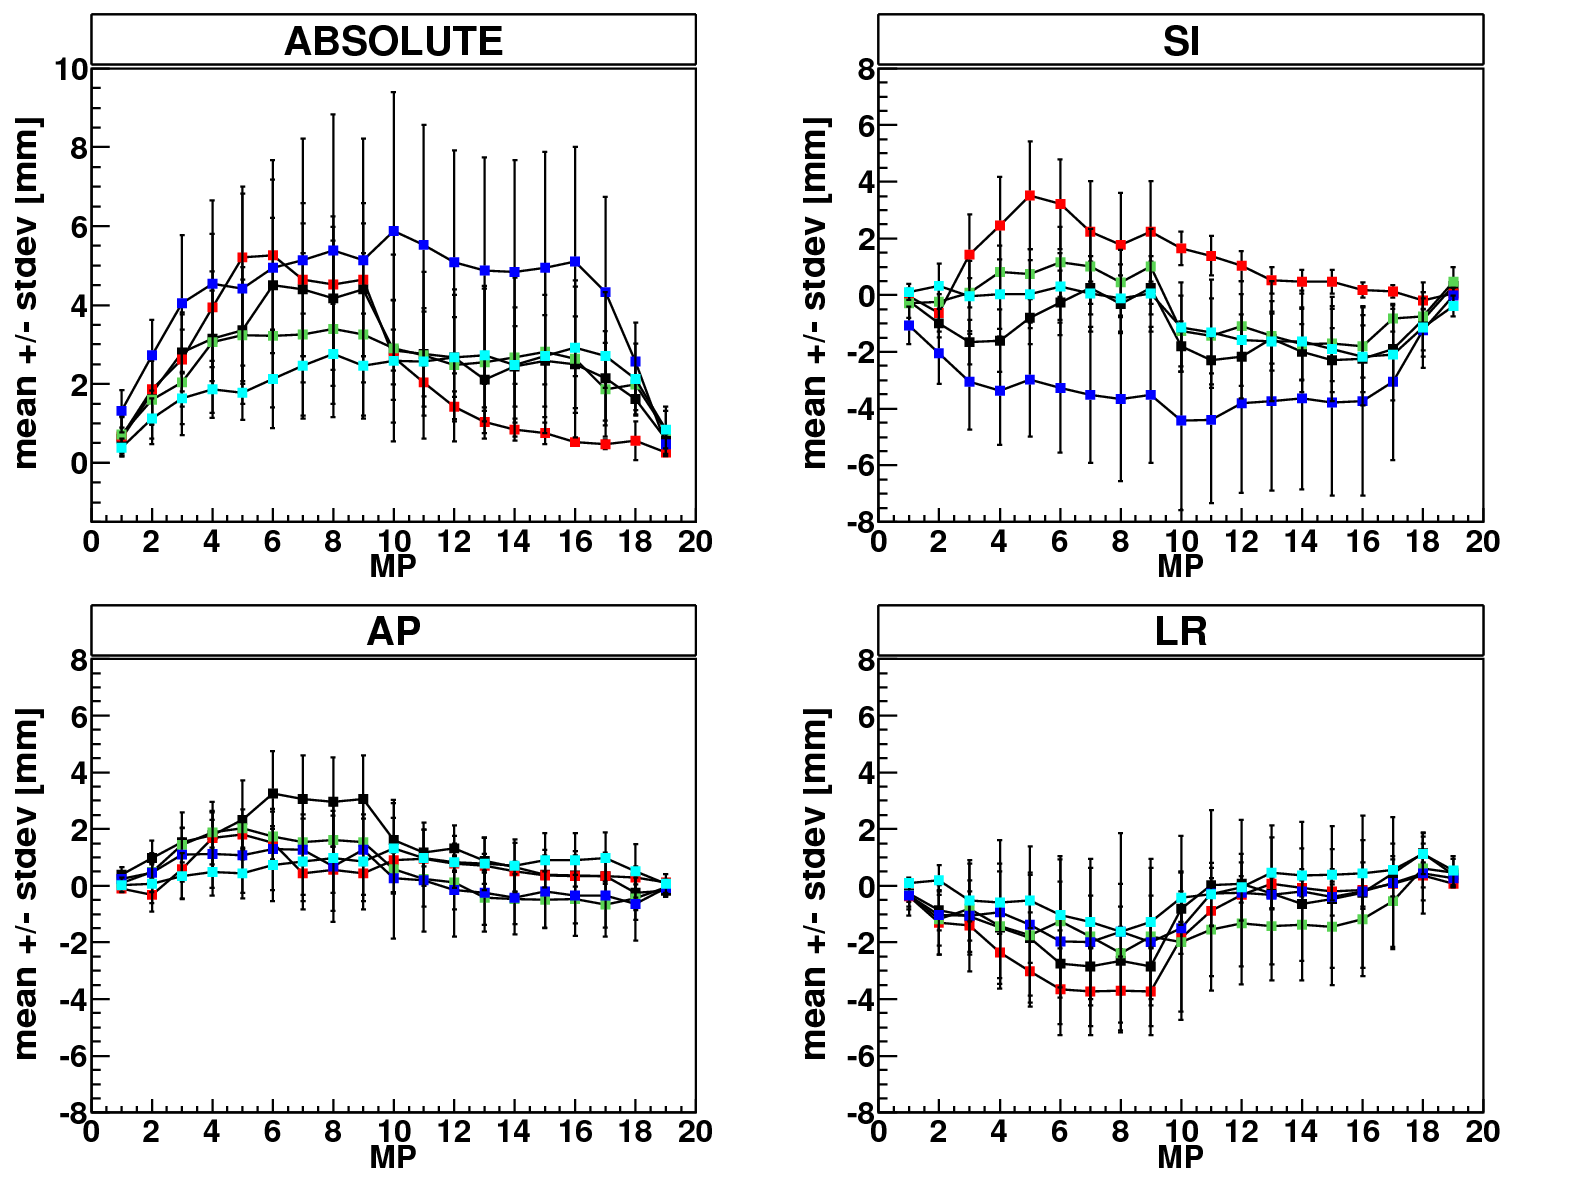
\includegraphics[scale=0.22]{MAYO_allPatients_HB_LPV.png}
\caption{Mean motion amplitude and standard deviation of LPV in each motion phase (MP) relative to the reference phase under influence of 
heartbeat for all patients (Patient 1: black, Patient 2: red, Patient 3: green, Patient 4: blue, Patient 5: turquois). 
The motion is shown in the three studied motion directions (SI: superior-inferior, AP: anterior-posterior, LR: left-right) and the absolute 
(ABS) displacment.}
\label{fig:motion_hb_lpv}
\end{center}
\end{figure}

\vspace*{-1.3cm}

\begin{figure}[H]
\begin{center}
 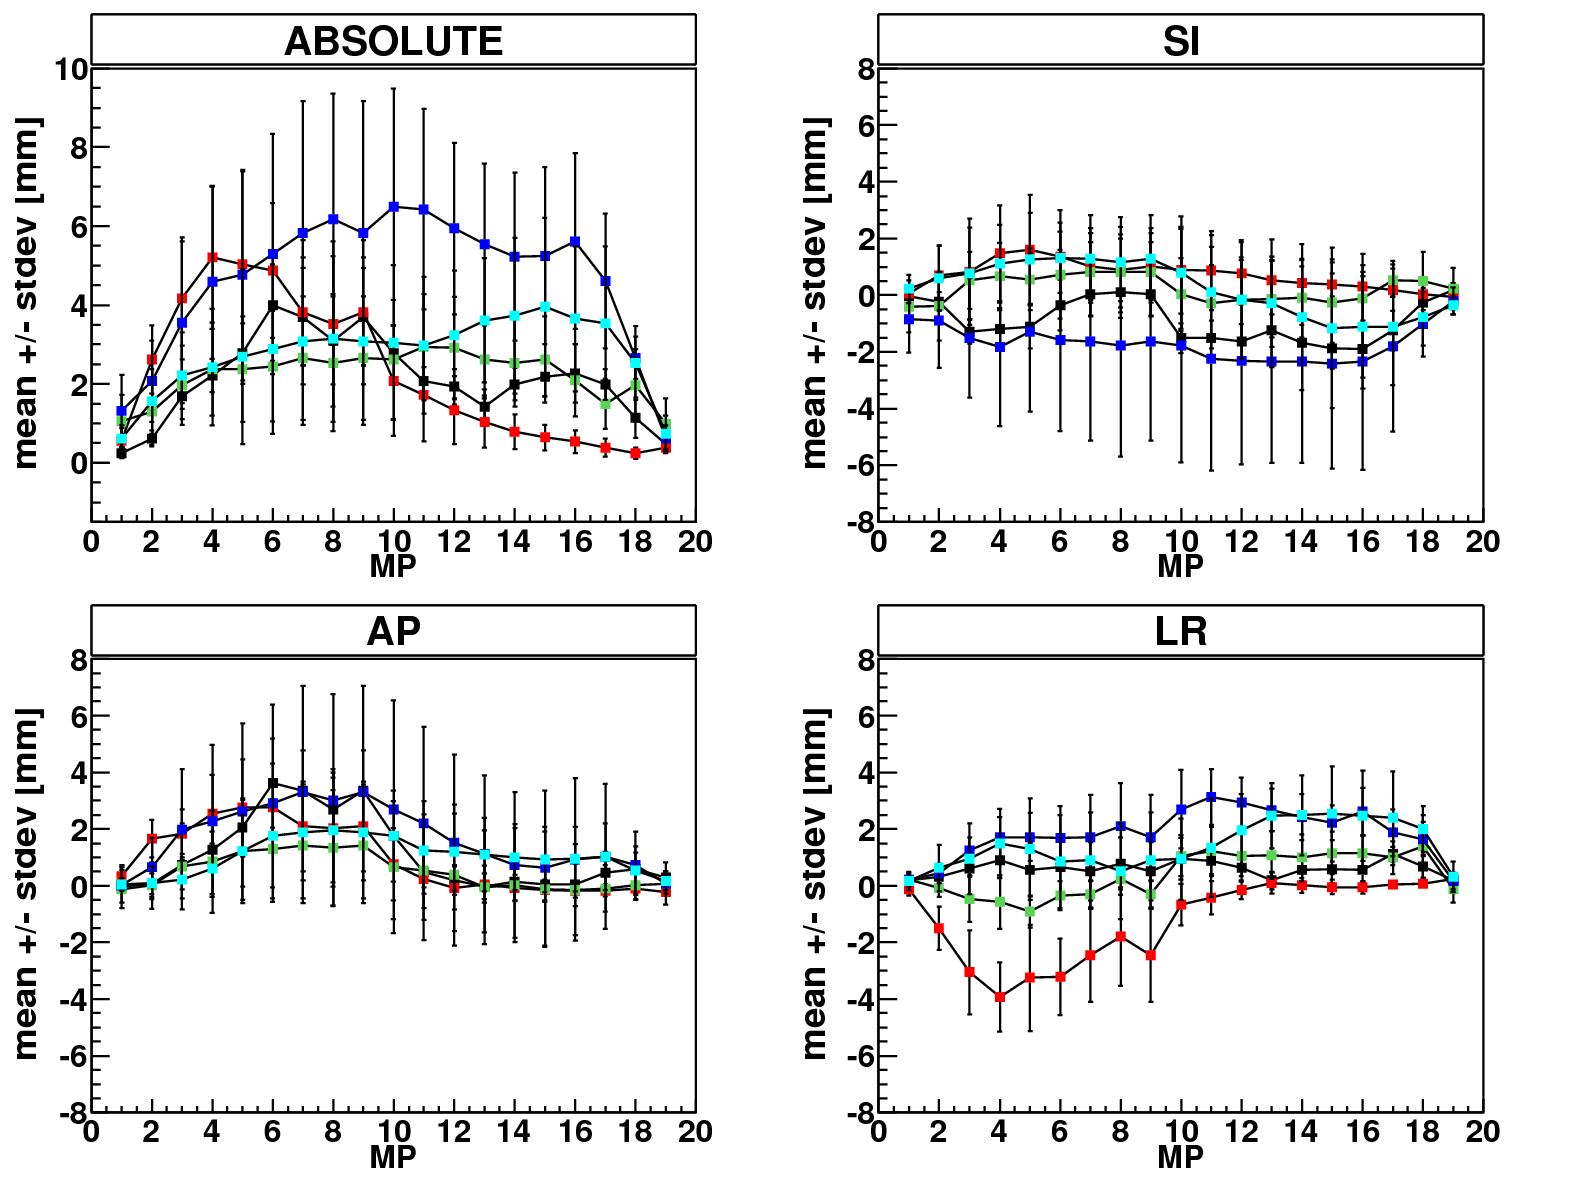
\includegraphics[scale=0.22]{MAYO_allPatients_HB_RPV.png}
\caption{Mean motion amplitude and standard deviation of RPV in each motion phase (MP) relative to the reference phase under influence of 
heartbeat for all patients (Patient 1: black, Patient 2: red, Patient 3: green, Patient 4: blue, Patient 5: turquois). }
\label{fig:motion_hb_rpv}
\end{center}
\end{figure}

\newpage

\vspace*{1cm}

\begin{table}[H]
  \centering
  \caption{Mean displacement of PVs over all motion phases (MP) in all patients and motion directions.}
  \begin{tabular}{|c|c|c|c|c|}
    \hline\hline
    Patient & LPV: ABS [mm] & LPV: SI [mm] & LPV: AP [mm] & LPV: LR [mm] \\
    \hline
    1 & 2.71 $\pm$ 1.18 & -1.17 $\pm$ 0.91 & 1.35 $\pm$ 1.08 & -0.89 $\pm$ 0.75 \\
    2 & 2.31 $\pm$ 1.14 & 1.16 $\pm$ 1.10 & 0.63 $\pm$ 0.53 & -1.38 $\pm$ 0.90 \\
    3 & 2.48 $\pm$ 1.75 & -0.36 $\pm$ 1.07 & 0.54 $\pm$ 0.78 & -1.18 $\pm$ 1.95 \\
    4 & 4.27 $\pm$ 2.54 & -3.07 $\pm$ 2.49 & 0.34 $\pm$ 1.43 & -0.78 $\pm$ 2.47 \\
    5 & 2.15 $\pm$ 1.23 & -0.75 $\pm$ 1.44 & 0.67 $\pm$ 1.10 & -0.18 $\pm$ 0.94 \\
    \hline\hline
    Patient & RPV: ABS [mm] & RPV: SI [mm] & RPV: AP [mm] & RPV: LR [mm] \\
   \hline
    1 & 2.12 $\pm$ 0.71 & -0.88 $\pm$ 0.65 & 1.11 $\pm$ 0.87 & 0.60 $\pm$ 0.60 \\
    2 & 2.25 $\pm$ 1.28 & 0.70 $\pm$ 1.15 & 0.96 $\pm$ 1.07 & -1.19 $\pm$ 1.01 \\
    3 & 2.22 $\pm$ 1.19 & 0.23 $\pm$ 1.25 & 0.50 $\pm$ 1.77 & 0.39 $\pm$ 0.70 \\
    4 & 4.62 $\pm$ 2.33 & -1.68 $\pm$ 3.12 & 1.67 $\pm$ 2.82 & 1.84 $\pm$ 0.94 \\
    5 & 2.77 $\pm$ 1.72 & 0.22 $\pm$ 1.77 & 1.03 $\pm$ 1.25 & 1.40 $\pm$ 1.40 \\
    \hline\hline
  \end{tabular}
  \label{tab:motion_pv}
\end{table}

\begin{table}[H]
  \centering
  \caption{Biggest absolute displacement of PVs with corresponding motion phase (MP) in all patients.}
  \begin{tabular}{|c|c|c|}
    \hline\hline
    Patient & LPV: max. ABS [mm] & MP \\
    \hline
    1 & 4.50 $\pm$ 1.72 & 06 \\
    2 & 5.26 $\pm$ 1.92 & 06 \\
    3 & 3.39 $\pm$ 2.24 & 08 \\
    4 & 5.52 $\pm$ 3.06 & 11 \\
    5 & 2.92 $\pm$ 1.54 & 16 \\
    \hline\hline
   Patient & RPV: max. ABS [mm] & MP \\
   \hline
    1 & 3.99 $\pm$ 1.40 & 06 \\
    2 & 5.20 $\pm$ 1.80 & 04 \\
    3 & 2.93 $\pm$ 1.35 & 11 \\
    4 & 6.49 $\pm$ 3.00 & 10 \\
    5 & 3.95 $\pm$ 3.95 & 15 \\
    \hline\hline
  \end{tabular}
  \label{tab:maxabs_pv}
\end{table}

\newpage

The overall displacement field between the extreme states of the ventricular displacement (motion phase three) and atrial displacement 
(motion phase eightteen) for two exemplary patients with a small motion amplitude (patient 5) and a large motion amplitude (patient 4) are 
shown in figure \ref{contour_plot_hb}. In order to visualize the location of the displacement, an axial cut of the reference state CT is 
underlayed. The absolute values of the displacement vectors are shown as contour plots. 

\begin{figure}[H]
\subfigure[Patient 4: max motion ventricle]{
 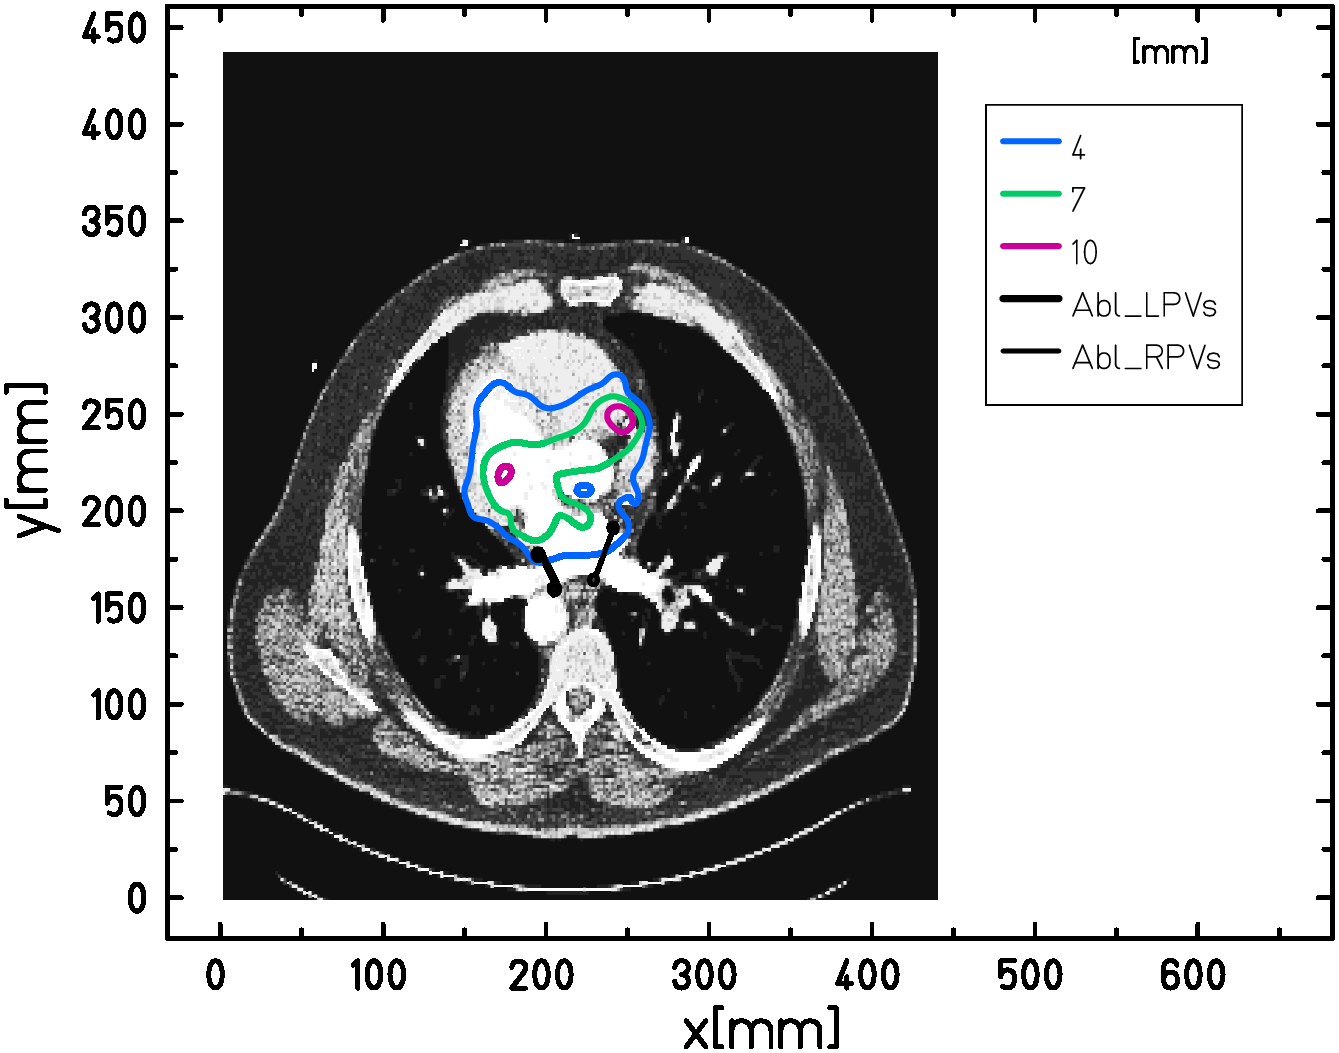
\includegraphics[scale=0.18]{Contour_z_abs_HB_Pat08_03_HUSkala_gedreht.png}
}
\subfigure[Patient 5: max motion ventricle]{
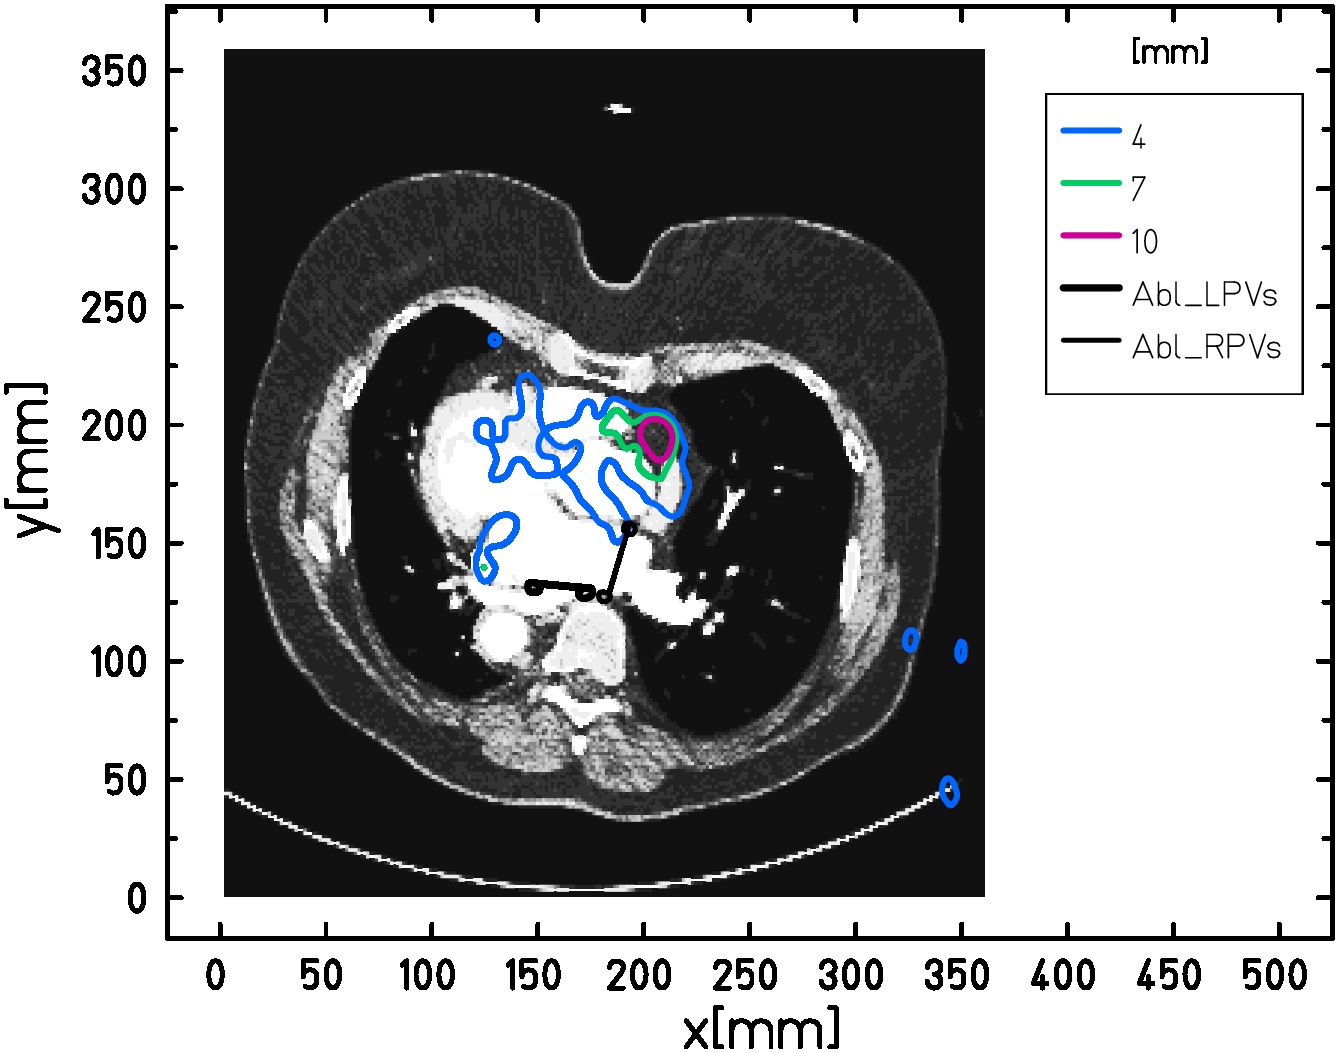
\includegraphics[scale=0.18]{Contour_z_abs_HB_Pat10_03_HUSkala_gedreht.png}
}
\subfigure[Patient 4: max motion atria]{
 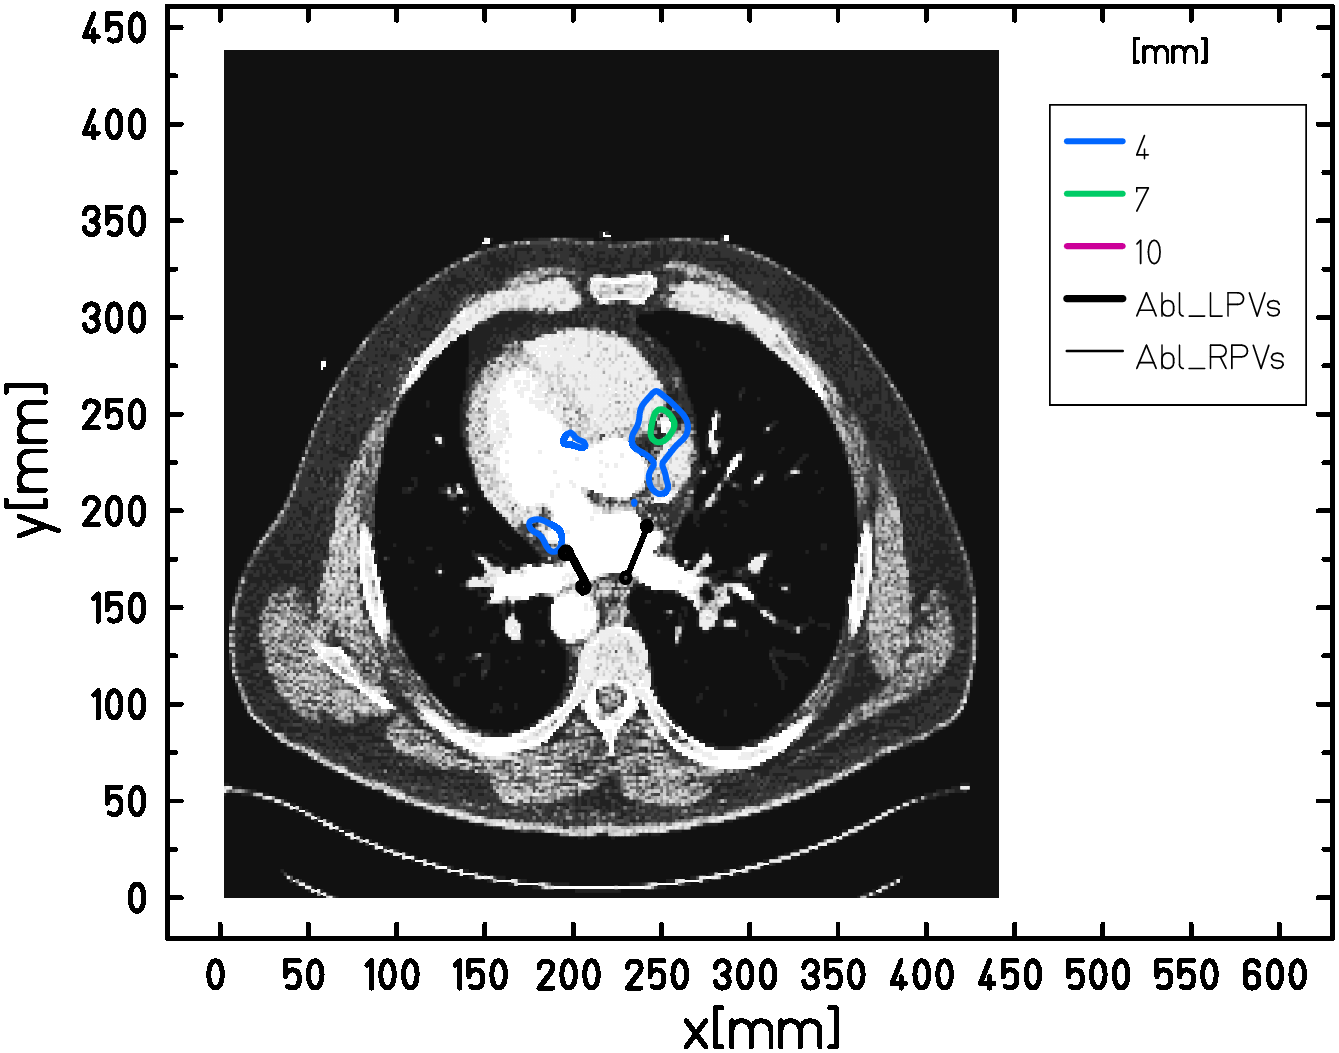
\includegraphics[scale=0.18]{Contour_z_abs_HB_Pat08_18_HUSkala_gedreht.png}
}
\subfigure[Patient 5: max motion atria]{
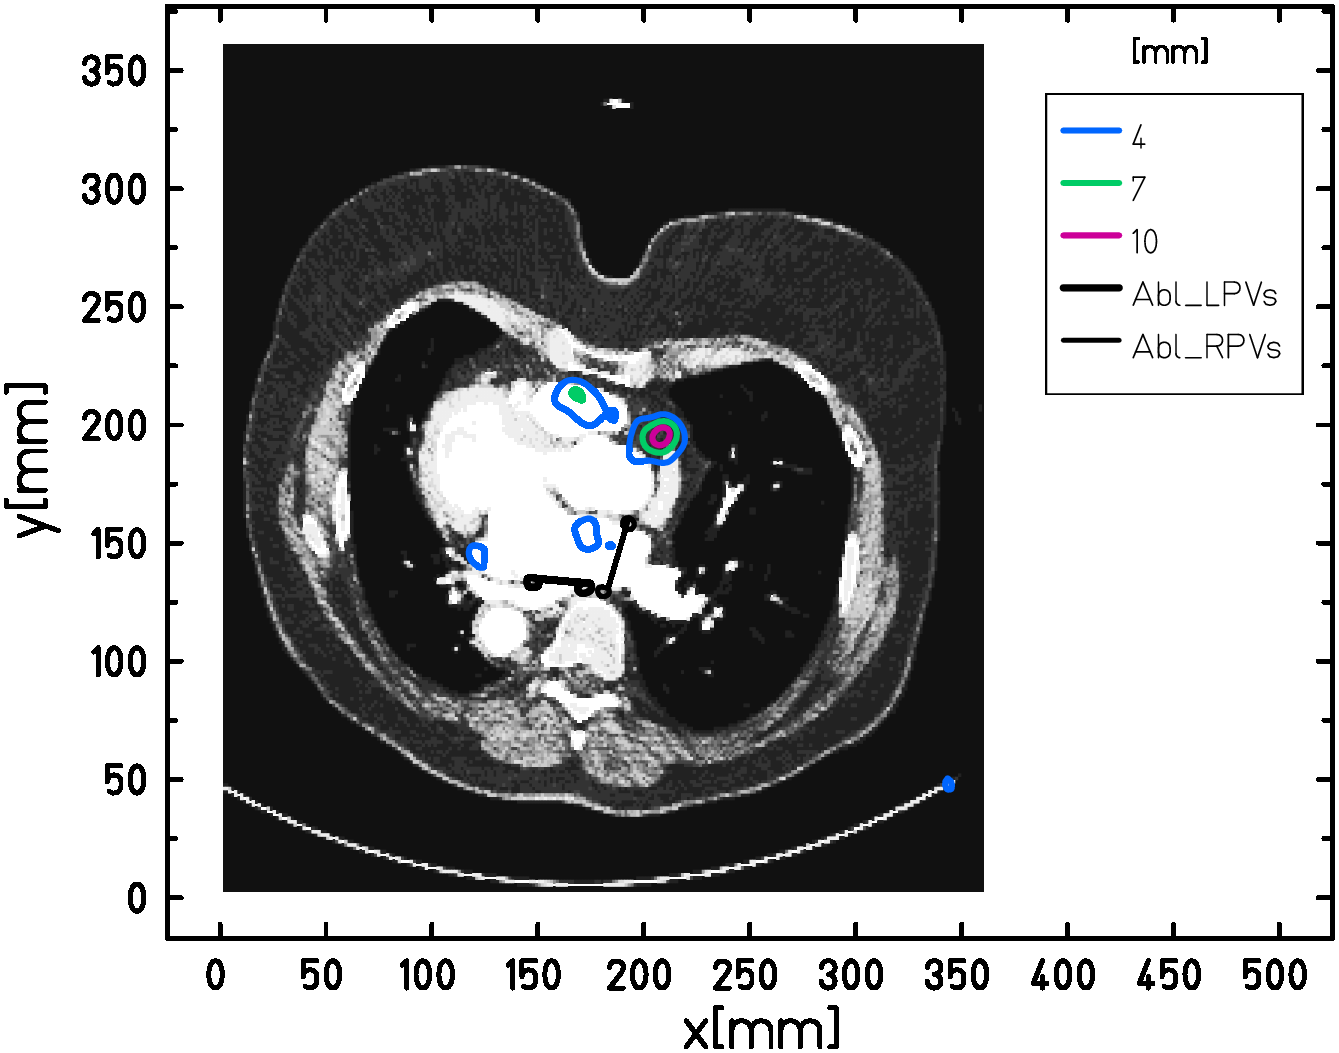
\includegraphics[scale=0.18]{Contour_z_abs_HB_Pat10_18_HUSkala_gedreht.png}
}
\caption{Axial slices of the reference state of the CT overlayed with the absolute values of the displacement field (obtained from 
deformable image registration) in the corresponding slice for heartbeat motion. In the top row the displacement from the motion phase with the 
maximal ventricle motion to the reference phase is shown, in the lower row the displacement from the motion phase with the maximal 
atrial motion, for Patient 4 and Patient 5, respectively.}
\label{contour_plot_hb}
\end{figure}


\newpage
\subsection{Motion mitigation techniques for heartbeat}

The absolute motion amplitudes of up to 5mm due to heartbeat are expected to yield dose inhomogeneities when not compensated for. The 
resulting interplay effect and dose deposition were studied for every patient for different motion patterns and different margins to the target 
volumes. The dose analysis values V95, V107 and D5-D95 were assessed and plotted. For comparison also the corresponding 
values for the 3D case (static) are shown. Due to the small motion amplitude, rescanning was studied as motion mitigation technique.  
The results of the stated dose values in case of rescanning with different rescan numbers will also be presented. 


\subsubsection{Dose deposition}
The dependencies of dose coverage and dose homogeneity on safety margin and rescan numbers are shown over all patients and the two 
target volumes, LPV and RPV, in figure \ref{static_interplay_rescanning_ALLpatients_KORR} over all patients and motion patterns. 
It can be shown that ten rescans yield a robust motion mitigation technique for the displacement of the PVs due to heartbeat motion. 
This will be studied in more detail in the following.\newline
\newline
A representative dose deposition for all studied techniques (static, interplay and rescanning with ten rescans) is shown exemplary for patient 
4 (as this is the patient with the largest PV motion amplitude both in LPV and RPV) in figure \ref{dose_pat08}. Rescanning and interplay 
are shown for a motion period of 0.7s and a starting phase of 0$^{\circ}$. The target volumes LPV and RPV were irradiated 
simultaneously and a margin of 3mm was added. \newline
\newline
Exemplary for patient 4, DVHs of the CTV for a static irradiation as well as interplay and ten rescans for different motion patterns and a 
target volume with 3mm safety margin are displayed in figure \ref{dvhs_pat08}. 
In order to assess the dose information of all patients the DVHs were analyzed and compared for dose steepness, dose coverage as well as 
over dosage. The average results over all patients with the resulting standard deviation can be seen in figure 
\ref{static_interplay_rescanning_ALL}. A more detailed analysis can be found in appendix \ref{app:human}, where the 
corresponding numerical values are shown (tables \ref{tab:Pat02_LPV} - \ref{tab:Pat10_RPV}).\newline
\newline
For interplay it can be seen that the results are slightly dependent on the used motion period and starting phase. This can be seen in the 
mean values of the resulting dose parameter values for different, underlying motion patterns. E.g. for LPV, the mean value of the dose 
coverage parameter over all patients is V95=(87.7 $\pm$ 7.4)\% for a motion with 1s period and a starting phase of 90$^{\circ}$ and 
(92.1 $\pm$ 4.3)\% for a motion with 0.7s period and a starting phase of 90$^{\circ}$, while for a motion with 0.7s period 
and a starting phase of 0$^{\circ}$ the dose coverage is found to be (90.4 $\pm$ 3.3)\%. 
Furthermore the result is also dependent on the studied safety margin, so that e.g. the dose coverage for a motion with 1s period 
and a starting phase of 90$^{\circ}$ is (94.6 $\pm$ 4.4)\% with 3mm safety margin. All these dependencies are also valid for 
the other studied dose analysis parameters, dose homogeneity and over dosage. The improvement of the dose coverage and dose homogeneity 
in relation to the size of the safety margin are also presented in figure \ref{static_interplay_rescanning_ALLpatients_KORR} (a and b). 
The dose homogeneity resulting from interplay as well as all rescanning irradiations was studied in relation to the used margin size and the 
proportion of variance explained resulted in $r^{2}$=0.35 (p<0.0001), hence favoring the application of the necessary safety margins. 
It becomes obvious that a safety margin of 3mm is already sufficient to drastically improve the outcome.\newline 
\newline
The underlying deformation map with its motion amplitude does not enable a prediction of the magnitude of the interplay effect. 
This was studied in more detail for the dose homogeneity, as these values were normally distributed. 
The proportion of variance explained between the maximal motion amplitude of the left and right PV (see table \ref{tab:maxabs_pv}) and 
the resulting D5-D95 values for all studied margins resulted in $r^{2}$=0.02 (p<0.0001).\newline 
\newline
As can be seen in figure \ref{static_interplay_rescanning_ALL} (as well as in more detail for all patients in appendix \ref{app:human:mmt}) 
rescanning yields improved results compared to interplay in all studied cases. This is valid for dose steepness, dose 
coverage as well as over dosage. Especially dose coverage and over dosage are comparable to the static results for all patient and motion patterns.  
Exemplary, the dose coverage of patient 4 (with the largest absolute displacement) will be discussed. V95 for a static irradiation of the 
LPV of patient 4 with 3mm safety margin is found to be 99.8\%. With a motion of 0.7s period length and a starting phase of 0$^{\circ}$ the value  
decreases to 90.0\%. With rescanning, V95 can be improved to 99.8\% with only five rescans. For RPV the static dose coverage 
with 3mm margin is found to be 100\% for this patient. With the stated motion and safety margin the dose coverage decreases to 97.0\%  
in case of interplay. Even though this is an acceptable value, the treatment gets more robust with rescanning and only five rescans are 
sufficient to increase the value to 100.0\%. The improvement of dose coverage and over dosage 
compared to interplay is valid for all studied rescan numbers, starting from the smallest studied rescan number of five, as shown here. 
Nevertheless, in some studied cases five rescans is not enough to yield results comparable to the static irradiation. 
This was studied in more detail for the dose coverage parameter V95. 
For example for the LPV irradiation with five rescans in patient 1 with a motion period of 1s and 90$^{\circ}$ starting phase (3mm safety 
margin) V95 results in a smaller dose coverage (93.2\%) than the static case (100\%). Even though this result is improved compared to 
interplay (86.9\%), a much better result can be gained with higher rescan numbers, starting with ten rescans (99.2\%). Also the results for 
dose homogeneity improves with higher rescan numbers. For a motion pattern of 0.7s period and 0$^{\circ}$ starting phase (3mm safety margin) 
in patient 4, the dose homogeneity in case of interplay is found to be 9.9\%. With five rescans a dose homogeneity of 5.5\% is yielded, which 
further decreases to 4.6\% with ten rescans, 4.4\% with fifteen rescans and 3.9\% with twenty rescans (compared to 3.9\% in the static irradiation). 
As the dose homogeneity was normally distributed, the relation between dose homogeneity and rescan number was analyzed. 
Thereby interplay was included as a rescan number of one. The explained variance was found to be $r^{2}$=0.37 (p<0.0001). 
It can thus be concluded that rescan numbers higher than five yield slightly better results, while ten rescans show results comparable to the 
static irradiation in all studied patient cases, for all studied safety margins and for all underlying motion patterns. This can 
also be seen in figure \ref{static_interplay_rescanning_ALLpatients_KORR} (c) where the dose coverage over all patients and margins 
is studied in relation to the used rescan number. It can be seen that while interplay (one rescan) results into a median of 8.9\% 
(75th percentile of 10.0\%), five rescans can reduce it to 6.1\% (8.1\%). With ten rescans this can be further improved to 4.1\% (5.9\%). 
Fifteen and twenty rescans on the other hand do not lead to an improved result compared to ten rescans (fifteen: 4.1\% (5.9\%), 
twenty: 4.0\% (5.7\%)).

\vspace*{-0.2cm}


\begin{figure}[H]
\centering
\subfigure[D5-D95 versus margin size]{
 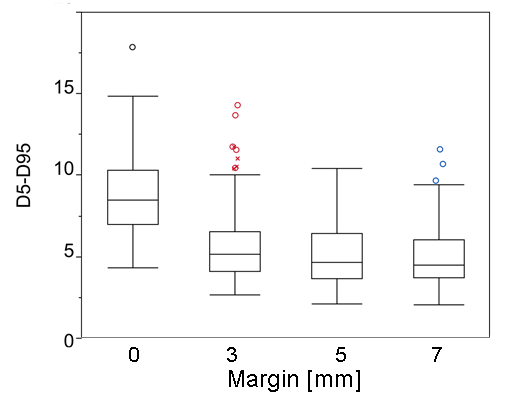
\includegraphics[scale=0.45]{D5-D95_vs_margin.png}
 }
 \subfigure[V95 versus margin size]{
 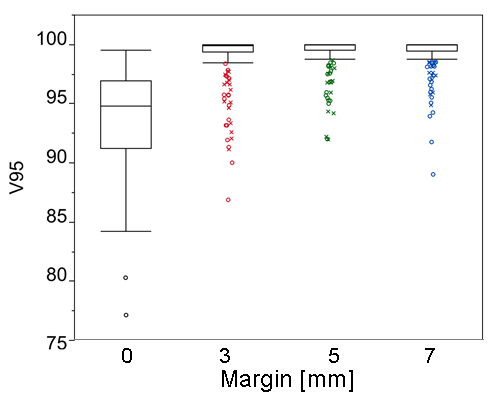
\includegraphics[scale=0.45]{V95_vs_margin.png}
 }
  \subfigure[D5-D95 versus rescan numbers]{
 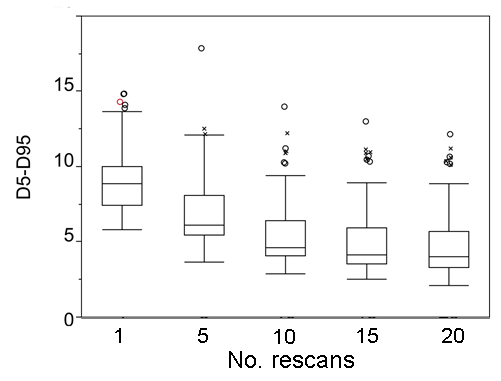
\includegraphics[scale=0.45]{D5-D95_vs_rescans.png}
}
  \subfigure[D5-D95 versus rescan numbers]{
 \includegraphics[scale=0.45]{V95_vs_rescans.png}
}
\caption{Boxplots of dose analysis parameters D5-D95 and V95 over all patient data sets and target volumes (LPV: circle and 
RPV: cross) depending on the used margins size (0mm: black, 3mm:red, 5mm: green, 7mm: blue) or the used rescan number (one rescan equals 
interplay, rescanning with five, ten, fifteen and twenty rescans). Minimum and maximum of the data is plotted within 1.5 times the
interquartile range, the other data points are stated as outliers. Figures are courtesy of Dr. Christian Graeff.}
\label{static_interplay_rescanning_ALLpatients_KORR}
\end{figure}

\newpage

 \begin{figure}[H]
 \begin{center}
\subfigure[static]{
 \includegraphics[scale=0.46]{Pat08_static_withLegend.png}
 }
\subfigure[interplay]{
 \includegraphics[scale=0.46]{Pat08_interplay_withLegend.png}
 }
 \subfigure[rescanning (10x)]{
 \includegraphics[scale=0.46]{Pat08_10rescans_withLegend.png}
 }
\caption{Dose distribution of patient 4 for static (a) as well as interplay (b) and ten rescans (c) for a motion period of 0.7s and a motion 
starting phase of 0$^{\circ}$. The target volume has an added margin of 3mm.}
\label{dose_pat08}
 \end{center}
\end{figure}

\newpage
% \vspace*{-0.3cm}

 \begin{figure}[H]
 \begin{center}
\subfigure[LPV]{
 \includegraphics[scale=0.28]{Pat08_LPV_allDVHs_newColor_withLegend.png}
 }
\subfigure[RPV]{
 \includegraphics[scale=0.28]{Pat08_RPV_allDVHs_newColor_withLegend.png}
 }
\caption{Dose volume histograms for CTV of patient 4 for 3mm safety margin irradiation (LPV (a) as well as RPV (b)) in case of static 
irradiation (black), interplay (dashed) and rescanning with ten rescans (solid). The motion patterns are shown in colors (1s 0: motion period of 1s 
and starting phase 0$^{\circ}$, 1s 90: motion period of 1s and starting phase 90$^{\circ}$, 07s 0: motion period of 0.7s 
and starting phase 0$^{\circ}$, 07s 90: motion period of 0.7s and starting phase 90$^{\circ}$.}
\label{dvhs_pat08}
 \end{center}
\end{figure}


\newpage
% \vspace*{-0.3cm}
\begin{figure}[H]
\subfigure[D5-D95: LPV]{
 \includegraphics[scale=0.18]{MAYO_CTV_LPV_D5D95.png}
 }
 \subfigure[D5-D95: RPV]{
 \includegraphics[scale=0.18]{MAYO_CTV_RPV_D5D95.png}
 }
 \subfigure[V95: LPV]{
 \includegraphics[scale=0.18]{MAYO_CTV_LPV_V95.png}
 }
\subfigure[V95: RPV]{
 \includegraphics[scale=0.18]{MAYO_CTV_RPV_V95.png}
 }
  \subfigure[V107: LPV]{
 \includegraphics[scale=0.18]{MAYO_CTV_LPV_V107.png}
 }
\subfigure[V107: RPV]{
 \includegraphics[scale=0.18]{MAYO_CTV_RPV_V107.png}
 }
\caption{Mean and standard deviation of dose analysis parameters D5-D95 (first row), V95 (middle row) and V107 (last row) over all patients. 
The LPV (left column) and RPV (right column) were studied seperately. Static (black) as well as interplay (red) and different rescanning 
numbers (5 times: blue, 10 times: green) were compared for different motion patterns and safety margins. For a better visualization the 
rescanning data points for each motion pattern are shifted and the result for fifteen and twenty rescans are not displayed.}
\label{static_interplay_rescanning_ALL}
\end{figure}

\newpage


\subsubsection{Irradiation time}
In figure \ref{irrTime_all} the mean irradiation time over all patients for different rescanning irradiations of LPV and RPV are shown for 
different safety margins and motion patterns. The duration for each beam entry channel (gantry angle of -45$^{\circ}$, 135$^{\circ}$ and 0$^{\circ}$) 
is plotted individually. It can be seen that the needed irradiation time increases with the used safety margin as the irradiated volume 
increases. The irradiation time is independent of the motion pattern but varies depending on the used beam entry channel. 
The stated results were achieved with a low intensity irradiation 
(minimal particle number of 5,000). For an irradiation with 3mm margin around LPV and RPV the overall treatment time is calculated to (13.71 $\pm$ 
0.94)min (see table \ref{tab:rescan_time}) with rescanning as motion mitigation technique for heartbeat motion. This time could be increased 
if a higher minimum particle number per beam spot (e.g. 75,000) was used, which needs to be studied. 

 \begin{figure}[H]
 \begin{center}
 \includegraphics[scale=0.2]{All_irrTime.png}
\caption{Mean and standard deviation of the irradiation time over all patients for different underlying motion patterns and beam entry 
channels.}
\label{irrTime_all}
 \end{center}
\end{figure}

\begin{table}[H]
  \centering
%   \footnotesize
  \caption{Mean irradiation time for LPV and RPV with a safety margin of 3mm over all patients.}
  \begin{tabular}{|c|c|c|}
    \hline\hline
    Gantry angle [$^{\circ}$] & time [min] & total [min] \\
    \hline
    -45 & 4.73 $\pm$ 0.93 & \\
    135 &  4.42 $\pm$ 0.94 & 13.71 $\pm$ 0.94\\
    0 & 4.56  $\pm$ 0.96 & \\
    \hline\hline
    \end{tabular}
  \label{tab:rescan_time}
\end{table}


\newpage

\section{Discussion}

In this chapter the influence of heartbeat motion on the PVs was studied and treatment planning studies with rescanning as motion 
mitigation technique were carried out. A detailed analysis of the dose depositions to the OAR was performed, with special 
emphasis on the irradiation of cardiac substructures. Beforehand, a study of the best suited field number and beam directions was  
conducted as well as an analysis of possible safety margin limitations. 


\subsection{Dose to critical structures}
\label{Discussion:doseOAR}

Concerning the dose deposition in OAR (esophagus, trachea, aorta and heart) dose-volume limits from SBRT were used. In SBRT 
treatment a high dose is applied in a single fraction and hence comparable to the here stated dose delivery of 25Gy physical 
dose in one treatment session. 
An extensive collection of dose-volume-limits for SBRT are presented in the study protocols of the Radiation Therapy Oncology Group (RTOG). 
The stated dose-volume limits for trachea (10.5Gy in 4cm$^{3}$) and aorta (31Gy in 10cm$^{3}$) were not exceeded for any of the studied field 
numbers and beam channel combinations. The same is valid while keeping the chosen three fields (couch angle of 90$^{\circ}$ 
and gantry angles of -45$^{\circ}$, 135$^{\circ}$ and 0$^{\circ}$) constant and changing the studied safety margins (0mm, 3mm, 5mm and 7mm). 
For the esophagus on the other hand, the dose-volume limits were much more critical. Most of the studied beam directions yielded a dose 
which exceeded the stated dose-volume limit (11.9Gy for 5cm$^{3}$). Hence IMPT(OAR) deliveries, including the esophagus in the 
optimization process, were necessary. With this delivery technique and the above stated beam direction, the dose to the esophagus could be 
drastically reduced. With restrictions to a maximum point dose of 70\% to the esophagus (IMPT(OAR)$_{R1}$, weightfactor of 75\%) only an 
irradiation of the PVs with 3mm safety margin resulted in a dose deposition into the esophagus which met the dose volume limit 
(median of 9.3Gy, 75th percentile: 12.1Gy). This result could be further improved with different IMPT parameters (IMPT(OAR)$_{R2}$, 
maximum dose of 30\% and weightfactor of 200\%), enabling a safe irradiation. Thus also safety margins higher then 3mm should result in an 
uncritical dose deposition to the esophagus. 
For the heart all beam channels, safety margins and delivery types (IMPT or IMPT(OAR)) exceeded the stated dose-volume limit (16Gy for 
15cm$^{3}$). This is due to the fact that the heart is not only an OAR but part of the target itself. Hence a closer look on the affected 
cardiac substructures and the relevance of these dose depositions on cardiac toxicity and late effects were given.\newline
\newline
QUANTEC (quantitative analysis of normal tissue effects in the clinic) \cite{QUANTEC10} offers an comprehensive literature review 
on the available data of the last 20 years and is meant as an update of the extensively used dose-limits proposed by Emami et al. 
\cite{Ema91}. In the QUANTEC publication by Gagliardi et al. \cite{Gag10} radiation dose-volume effects in the heart are presented. 
It is stated that radiation-induced cardiac diseases are distinguished between acute injuries like pericarditis\footnote{inflammation 
of the sac containing the heart}, which can turn into a chronic disease, and late injuries which manifest months or even 
years after radiation exposure. Typical late injuries are congestive heart failure\footnote{heart is unable to maintain sufficient 
blood flow}, ischemia,
coronary artery disease and myocardial infarction. 
It was summarized that it remains uncertain which region of the heart is most important for radiation induced tissue toxicities. 
But it is stated that the risk of cardiac events is probably related to both dose and irradiated volume. 
Pericarditis seems to be related to left ventricle (LV) irradiation, and it was found that LV shielding was able to drastically 
reduce the incidence rate \cite{Carm76}. It was stated that a mean cardiac dose of 27.1Gy and maximum dose of 47Gy seem to act as 
predictors for pericarditis \cite{Mar98}. 
Wei et al. \cite{Wei08} stated another discriminator for pericarditis which was found to be V30 < 46\%, which translates in a mean 
pericardial dose of less than 26Gy. For coronary and ischemic events relevant substructures are assumed to be coronary arteries on 
the left ventricle (LCA) \cite{Nie07} \cite{Tay07} \cite{Tay08}. Furthermore it is stated that excess deaths from heart disease are observed 
in patients receiving more than 42Gy \cite{Han93} and that aortic and mitral stenosis incidences increased above a threshold dose of 
30Gy \cite{Tay07}. For long term cardiac mortality an increased rate was only observed at whole heart doses above 30Gy \cite{Han93}.\newline
\newline
Hooning et al. \cite{Hoo07} studied the cardiovascular disease incidence in more than 4000 breast cancer survivors 
after a follow-up period of more than 10 years as patients were treated from 1970 through 1986. It was the first study to examine the 
effects of cardiovascular risk factors in combination to radiotherapy. They found that the risk of congestive heart failure was 
significantly increased when the patients had received chemotherapy (95\% confidence interval of 1.25 to 2.73) and that smoking drastically 
increased the risk of the patients to suffer a myocardial infarction (95\% confidence interval of 2.03 to 4.55). Concerning 
radiotherapy they stated that a higher mean dose to the whole heart resulted in an increased risk of congestive heart failure and 
that an irradiation of the left vs right chest wall (thus more heart volume and in particular including the LV and apex) led to an 
increased risk of myocardial infarction.\newline
\newline
A recent study by Darby et al. \cite{Dar13} investigated more than 2000 breast cancer patients treated in between 1958 and 2001 
for coronary events like myocardial infarction, coronary revascularization or death from ischemic heart disease. The found a mean 
heart dose of 4.9Gy (0.03Gy to 27.72Gy) and that the rates of major coronary events increased linearly with the mean heart dose. 
They stated an increase of incidences by 7.4\% per Gy (95\% confidence interval of 2.9 to 14.5) after five years post radiotherapy.
\newpage
For the here studied seventeen beam channel combinations, applying a physical dose of 25Gy, the mean dose to the heart of all five studied 
patients was found to have a median of 1.3Gy (75th percentile of 1.5Gy). The median over the maximal point dose was 
found to be up to 26.6Gy (75th percentile: 27.1Gy), while in general less than 30\% of the heart was irradiated. 
With the chosen field number of three beam channels with a couch angle of 90$^{\circ}$ and gantry angles of -45$^{\circ}$, 
135$^{\circ}$ and 0$^{\circ}$, the mean dose was found to be negligible (median of 1Gy, 75th percentile of up to 1.5Gy) in all 
studied patient cases. The median mean dose over all patients did not increase with increasing safety margin for both IMPT(OAR) deliveries. 
As the LV, and with it especially the LCA, are assumed to be radiosensitive structures within the heart the dose 
depositions to these structures were analyzed in more detail. It was found that three beam channel directions were best suited to yield a lower 
mean dose deposition in the LCA. Due to robustness criteria of the treatment delivery the above stated beam channel combination was 
chosen. With this delivery direction and an IMPT(OAR)$_{R2}$ treatment it was found that the mean dose to the LCA was, dependent on the 
used safety margin, 0.2Gy(75th percentile: 0.7Gy) with no margin, 0.4Gy (75th percentile: 1.7Gy) for 3mm margin, 1.0Gy (75th percentile: 
2.0Gy) for 5mm and 1.3Gy (75th percentile: 2.8Gy) for 7mm. The maximum point dose to the LCA with these beam channels nevertheless led to 
an increased dose in the left chamber compared to the right site. This is due to the proximity of the upper LCA branches 
to the LPV target site. 

\subsection{Beam channel directions and safety margins}
In general, it can be stated that field number and beam direction always result in a trade-off between dose to the OAR, irradiation time and 
robustness. While less fields and hence beam directions shorten the treatment time, it does lead to a less robust treatment. In case OAR are 
displaced during the treatment (intrafractional motion, see Introduction) or move in between CT image acquisition and irradiation 
(interfractional motion) beam channels with a large angle in between them are more robust, as not all fields are affected by this displacement 
and hence only a small dose would be shifted. Furthermore, opposite fields (like -45$^{\circ}$ and 135$^{\circ}$ (see figure 
\ref{gantrydirection}) are more robust against potential range uncertainties and should hence be favored. Due to this reason, combined with 
the smaller LCA dose deposition in case of three field numbers, a couch angle of 90$^{\circ}$ and gantry angles of -45$^{\circ}$, 
135$^{\circ}$ and 0$^{\circ}$ were selected for the safety margin limitation studies as well as the motion mitigation treatment plans. 
Concerning safety margins, which need to be applied in order to account for possible deviations in between treatment planning and dose 
delivery, it can be stated that only a small margin tolerance was observed. This is due to the difficult position of the PVs close to 
radiosensitive structures like the esophagus and especially the heart. With IMPT treatment a delivery with 3mm safety margin was found to 
fulfill all the needed requirements. A more realistic safety margin of 5mm could be achieved with more restricted parameters in the IMPT 
optimization. 


\subsection{Movement of PVs in cardiac cycle}

Lickfett et al. \cite{Lic05} analyzed the volume changes and displacement of the PVs in 25 healthy volunteers with MRI images. They 
studied the posterior edge of the PV orifice and observed that the size and location changed considerably during the cardiac cycle. 
Displacements of up to 7.2mm were found and it could be concluded that the motion amplitudes were bigger in the coronal (left-right) 
than in the sagittal (anterior-posterior) direction. In more detail this largest coronal movement was found in the left superior PV, 
while the largest sagittal motion was observed in the right superior PV with 3.9mm. The smallest saggital displacement was 2.5mm in the 
left anterior PV. They suspected that the reason for movement is not resulting from a single influence, but is rather a mix of PV 
contraction, atrial contraction and ventricular force. The movement of PV due to heartbeat is also relevant for catheter ablation. Based 
on the stated finding Lickfett et al. recommended to keep a 5mm distance from the PV orifice during PV encircling ablation in order to 
reduce the risk for PV stenosis. 
Patel et al. \cite{Pat08} studied the MRI images of 30 patients in sinus rhythm with paroxysmal atrial fibrillation. They  
stated that the mean displacement of the pulmonary veins was small. The left lower PV was found to move (2.7 $\pm$ 1.2)mm, the left upper PV 
(2.1 $\pm$ 1.1)mm, the right lower PV (1.9 $\pm$ 1.1)mm and the right upper PV (2.3 $\pm$ 1.0)mm.\newline 
\newline
In the here studied patient cohort of five AF patients no differentiation between the upper and lower PVs was carried out. 
The motion was assessed for the whole potential ablation site of LPV and RPV, respectively. Similar to the study by Patel et al. only a small 
mean displacement was found, resulting in an average absolute displacement of less than 3mm (LPV: (2.71 $\pm$ 1.57)mm, RPV: (2.62 $\pm$ 1.41)mm). 
Even though a tendency to a higher motion in AP direction could be observed, the contributions of the other motion directions 
were in the same order of magnitude (up to 1mm). Hence no dominant motion direction could be determined. 
The motion phases of the heartbeat gated CT scan were based on the ECG trace and resulted in a division of a single heartbeat. Thus the motion 
phases could be directly assigned to the contraction (systole) and dilatation (diastole) of both atria and ventricles. 
Nevertheless no motion phase could be assessed to yield the maximum displacement. This reinforces the hypothesis by Lickfett et al. that the 
underlying heartbeat motion, which causes the PVs to move, is much more complex. 

\newpage

\subsection{Rescanning as motion mitigation technique}

The small target volume displacement due to heartbeat led to small interplay effects, where the dose coverage was found 
to have V95 values smaller than 95\% in only 31\% of the studied cases. This result could be already improved by using safety margins, as 
71\% of these cases were irradiations with no safety margin and only 3\% of the stated cases were irradiations with safety margins of 
5mm or more. Nevertheless also irradiations with a safety margin of 7mm were found to have a V95 of 89\% in some cases (e.g. 
in the irradiation of the LPV in patient 4 with a motion period of 1s and a starting phase of 90$^{\circ}$). In order to 
guarantee a robust and conformal irradiation a motion mitigation technique was hence needed. Rescanning was studied 
and it can be concluded that this technique yields good results. \newline
\newline
Regarding dose coverage V95 values were higher than 99\% in 96.3\% of all studied cases with a safety margin of 3mm or higher. 
The minimum dose coverage over all studied cases with safety margin was found in patient 1, in the irradiation of the LPV with a margin 
of 3mm and an underlying motion of 1s period and 90$^{\circ}$ starting phase (V95=93.2\%). This result was obtained with five rescans. 
With higher rescans the dose coverage could be improved, so that only 1.5\% of the studied cases with ten or more rescans had a dose coverage 
smaller than 99\% (minimum: 97.1\%; 10 rescans in patient 1, 7mm safety margin and motion of 1s period and 90$^{\circ}$ starting phase). 
The dose coverage for rescans without safety margin was worse, resulting in 93.1\% cases under 99\%. In comparison, the static irradiations 
without safety margin resulted in a V95<99\% in only 17\% of the cases. 
V107 values higher than 0\% were obtained in 7.3\% of all cases with safety margin (maximum of V107=3.7\% in the LPV of patient 3 
with safety margin of 5mm, 5 rescans and motion of 1s period and 0$^{\circ}$ starting phase) compared to 
28.8\% of cases without safety margin (maximum: V107=8.0\% for the LPV of patient 2 with 5 rescans and motion of 1s period 
and 0$^{\circ}$ starting phase. This could be reduced to V107=2.9\% with 10 rescans). With safety margin, the dose homogeneity D5-D95 
did not exceed 8.9\%. Without safety margin D5-D95 did not exceed 10.2\%. Both of these values were achieved with 5 rescans and could be 
improved with 10 rescans (with safety margin to less than 7\% and without to less than 9\%). It can hence be concluded that additional 
safety margins enable a more robust and successful treatment delivery. However, if possible, these margins should be kept as small 
as technical feasible, as it increases the dose deposition in OARs. Regarding rescan numbers ten rescans yield improved results compared 
to five rescans. These results are not significantly improved with rescan numbers higher than ten.\newline 
\newline
All these results were found for slice-by-slice rescanning, which means that each IES is irradiated independently with the predefined number 
of rescans and the adapted particle numbers. In this case the treatment time is not prolonged. It needs to be studied if other rescanning 
techniques like breath-sampled rescanning \cite{Sec09} or phase-controlled rescanning \cite{Fur07}, where the rescanning of the individual IES 
are sampled according to the motion phase of the breathing period, are applicable to cardiac motion (ECG-sampled rescanning) and if this 
method would result in the need of fewer rescan numbers. 

\section{Conclusion}

The PVs were found to move due to heartbeat with an amplitude of up to 6mm. 
This displacement creates interplay effects when irradiated with scanned carbon ions. Rescanning as motion mitigation technique was studied. 
It yields improved dose coverage and dose homogeneity compared to interplay in all studied patient cases, motion patterns and 
for all safety margins. It is thus an adequate motion mitigation technique for the irradiation of PVs under influence of heartbeat motion. 
A rescan number of ten is sufficient to obtain results comparable to the static irradiation. 
For the treatment delivery, IMPT dose optimization together with a rather small safety margin (of e.g. 3mm) results in dose depositions in the 
OARs (like esophagus as well as in the cardiac substructures) which are considered tolerable. In order to achieve this an ion gantry, 
such as the one at HIT, is needed, as it allows for ion beam entry channels which better spare the critical structures. 



%%%%%%%%%%%%%%%%%%%%%%%%%%%%%%%%%%%%%%%%%%%
%%%%%%%%%%%%%% APPENDIX %%%%%%%%%%%%%%%%%%%
%%%%%%%%%%%%%%%%%%%%%%%%%%%%%%%%%%%%%%%%%%%

\appendix

\chapter{Appendix of chapter 3}
\label{app:human}

%%%%%%%%%%%%%%%%%%%%
%%%%%% MOTION %%%%%%
%%%%%%%%%%%%%%%%%%%%
\section{Motion of PV due to heartbeat}
\label{app:human:motion}

The mean relative displacement and standard deviation of the target volumes (LPV and RPV) to the reference phase zero will be shown for the three studied motion 
directions (SI: superior-inferior, AP: anterior-posterior, LR: left-right) and the absolute (ABS) displacement. 

\begin{table}[htbp]
  \centering
  \tiny
  \caption{Patient 1, LPV: Mean and standard deviation of target motion in all phases of the heartbeat, relative to the reference phase.}
  \begin{tabular}{|c|c|c|c|c|}
    \hline\hline
    motion phase\rule{0pt}{2.6ex}\rule[-1.2ex]{0pt}{0pt} & ABS [mm] & SI [mm] & AP [mm] & LR [mm]\\
    \hline 
01& 0.62 $\pm$ 0.27& -0.22 $\pm$ 0.15& 0.39 $\pm$ 0.26& -0.28 $\pm$ 0.30 \\
02& 1.78 $\pm$ 0.81& -1.00 $\pm$ 0.48& 0.97 $\pm$ 0.62& -0.86 $\pm$ 0.71 \\
03& 2.79 $\pm$ 0.98& -1.65 $\pm$ 0.78& 1.55 $\pm$ 1.03& -1.08 $\pm$ 0.87 \\
04& 3.15 $\pm$ 1.22& -1.61 $\pm$ 1.11& 1.78 $\pm$ 1.19& -1.48 $\pm$ 0.91 \\
05& 3.36 $\pm$ 1.28& -0.79 $\pm$ 0.93& 2.32 $\pm$ 1.39& -1.83 $\pm$ 0.90 \\
06& 4.50 $\pm$ 1.72& -0.27 $\pm$ 1.13& 3.25 $\pm$ 1.49& -2.76 $\pm$ 1.19 \\
07& 4.39 $\pm$ 1.68& 0.26 $\pm$ 0.93& 3.05 $\pm$ 1.56& -2.84 $\pm$ 1.15 \\
08& 4.17 $\pm$ 1.82& -0.32 $\pm$ 1.02& 2.95 $\pm$ 1.58& -2.64 $\pm$ 1.19 \\
09& 4.39 $\pm$ 1.68& 0.26 $\pm$ 0.93& 3.05 $\pm$ 1.56& -2.84 $\pm$ 1.15 \\
10& 2.85 $\pm$ 1.26& -1.81 $\pm$ 0.88& 1.61 $\pm$ 1.42& -0.82 $\pm$ 0.61 \\
11& 2.76 $\pm$ 1.08& -2.30 $\pm$ 0.98& 1.18 $\pm$ 1.04& 0.02 $\pm$ 0.24 \\
12& 2.68 $\pm$ 1.02& -2.16 $\pm$ 1.05& 1.31 $\pm$ 0.82& 0.06 $\pm$ 0.29 \\
13& 2.11 $\pm$ 0.71& -1.53 $\pm$ 0.89& 0.88 $\pm$ 0.82& -0.28 $\pm$ 0.56 \\
14& 2.44 $\pm$ 1.02& -2.01 $\pm$ 0.99& 0.66 $\pm$ 0.86& -0.65 $\pm$ 0.61 \\
15& 2.58 $\pm$ 1.16& -2.29 $\pm$ 1.12& 0.39 $\pm$ 0.88& -0.46 $\pm$ 0.59 \\
16& 2.49 $\pm$ 1.23& -2.25 $\pm$ 1.18& 0.36 $\pm$ 0.85& -0.24 $\pm$ 0.57 \\
17& 2.15 $\pm$ 1.20& -1.91 $\pm$ 1.06& 0.33 $\pm$ 0.85& 0.44 $\pm$ 0.48 \\
18& 1.61 $\pm$ 0.41& -0.88 $\pm$ 0.38& -0.26 $\pm$ 0.60& 1.15 $\pm$ 0.33 \\
19& 0.60 $\pm$ 0.20& 0.32 $\pm$ 0.19& -0.18 $\pm$ 0.21& 0.39 $\pm$ 0.20 \\
    \hline\hline
  \end{tabular}
\end{table}


\begin{table}[htbp]
  \centering
  \tiny
  \caption{Patient 1, RPV: Mean and standard deviation of target motion in all phases of the heartbeat, relative to the reference phase.}
  \begin{tabular}{|c|c|c|c|c|}
    \hline\hline
    motion phase\rule{0pt}{2.6ex}\rule[-1.2ex]{0pt}{0pt} & ABS [mm] & SI [mm] & AP [mm] & LR [mm]\\
    \hline
01& 0.25 $\pm$ 0.13& -0.03 $\pm$ 0.12& -0.02 $\pm$ 0.14& 0.18 $\pm$ 0.11 \\
02& 0.62 $\pm$ 0.20& -0.23 $\pm$ 0.33& 0.06 $\pm$ 0.37& 0.31 $\pm$ 0.17 \\
03& 1.68 $\pm$ 0.31& -1.28 $\pm$ 0.42& 0.73 $\pm$ 0.40& 0.61 $\pm$ 0.24 \\
04& 2.22 $\pm$ 0.42& -1.18 $\pm$ 0.73& 1.26 $\pm$ 0.65& 0.91 $\pm$ 0.54 \\
05& 2.77 $\pm$ 0.76& -1.11 $\pm$ 0.77& 2.05 $\pm$ 1.02& 0.57 $\pm$ 0.94 \\
06& 3.99 $\pm$ 1.40& -0.35 $\pm$ 0.90& 3.63 $\pm$ 1.57& 0.65 $\pm$ 0.93 \\
07& 3.70 $\pm$ 1.24& 0.04 $\pm$ 0.80& 3.36 $\pm$ 1.41& 0.51 $\pm$ 1.02 \\
08& 3.10 $\pm$ 1.12& 0.12 $\pm$ 0.72& 2.68 $\pm$ 1.31& 0.79 $\pm$ 0.92 \\
09& 3.70 $\pm$ 1.24& 0.04 $\pm$ 0.80& 3.36 $\pm$ 1.41& 0.51 $\pm$ 1.02 \\
10& 2.77 $\pm$ 0.71& -1.52 $\pm$ 0.52& 1.77 $\pm$ 1.01& 0.95 $\pm$ 0.74 \\
11& 2.08 $\pm$ 0.34& -1.51 $\pm$ 0.61& 0.49 $\pm$ 0.77& 0.87 $\pm$ 0.47 \\
12& 1.93 $\pm$ 0.45& -1.64 $\pm$ 0.62& 0.20 $\pm$ 0.53& 0.64 $\pm$ 0.31 \\
13& 1.42 $\pm$ 0.44& -1.25 $\pm$ 0.57& -0.02 $\pm$ 0.45& 0.18 $\pm$ 0.31 \\
14& 1.99 $\pm$ 0.41& -1.68 $\pm$ 0.63& 0.13 $\pm$ 0.64& 0.55 $\pm$ 0.45 \\
15& 2.18 $\pm$ 0.49& -1.87 $\pm$ 0.72& 0.05 $\pm$ 0.62& 0.59 $\pm$ 0.49 \\
16& 2.27 $\pm$ 0.74& -1.90 $\pm$ 1.00& 0.04 $\pm$ 0.75& 0.57 $\pm$ 0.45 \\
17& 1.98 $\pm$ 0.40& -1.25 $\pm$ 0.69& 0.46 $\pm$ 0.73& 1.11 $\pm$ 0.26 \\
18& 1.14 $\pm$ 0.51& -0.27 $\pm$ 0.38& 0.58 $\pm$ 0.59& 0.68 $\pm$ 0.42 \\ 
19& 0.48 $\pm$ 0.21& 0.18 $\pm$ 0.24& 0.28 $\pm$ 0.23& 0.20 $\pm$ 0.13 \\
    \hline\hline
  \end{tabular}
\end{table}


\begin{table}[htbp]
  \centering
    \tiny
  \caption{Patient 2, LPV: Mean and standard deviation of target motion in all phases of the heartbeat, relative to the reference phase.}
  \begin{tabular}{|c|c|c|c|c|}
    \hline\hline
    motion phase\rule{0pt}{2.6ex}\rule[-1.2ex]{0pt}{0pt} & ABS [mm] & SI [mm] & AP [mm] & LR [mm]\\
    \hline
01& 0.67 $\pm$ 0.48& -0.03 $\pm$ 0.21& -0.10 $\pm$ 0.17& -0.38 $\pm$ 0.67 \\
02& 1.86 $\pm$ 0.88& -0.62 $\pm$ 0.66& -0.32 $\pm$ 0.59& -1.31 $\pm$ 1.12 \\
03& 2.62 $\pm$ 1.20& 1.43 $\pm$ 1.41& 0.59 $\pm$ 1.06& -1.39 $\pm$ 0.94 \\
04& 3.94 $\pm$ 1.86& 2.46 $\pm$ 1.71& 1.68 $\pm$ 0.92& -2.35 $\pm$ 0.92 \\
05& 5.21 $\pm$ 1.80& 3.52 $\pm$ 1.90& 1.82 $\pm$ 0.61& -3.03 $\pm$ 1.23 \\
06& 5.26 $\pm$ 1.92& 3.21 $\pm$ 1.58& 1.51 $\pm$ 0.58& -3.65 $\pm$ 1.62 \\
07& 4.64 $\pm$ 1.94& 2.25 $\pm$ 1.77& 0.44 $\pm$ 0.76& -3.74 $\pm$ 1.53 \\
08& 4.52 $\pm$ 1.72& 1.78 $\pm$ 1.84& 0.57 $\pm$ 0.82& -3.71 $\pm$ 1.47 \\ 
09& 4.64 $\pm$ 1.94& 2.25 $\pm$ 1.77& 0.44 $\pm$ 0.76& -3.74 $\pm$ 1.53 \\
10& 2.68 $\pm$ 0.70& 1.66 $\pm$ 0.59& 0.90 $\pm$ 0.27& -1.84 $\pm$ 0.56 \\
11& 2.03 $\pm$ 0.61& 1.39 $\pm$ 0.70& 0.96 $\pm$ 0.28& -0.89 $\pm$ 0.51 \\
12& 1.43 $\pm$ 0.38& 1.03 $\pm$ 0.53& 0.78 $\pm$ 0.24& -0.32 $\pm$ 0.28 \\
13& 1.03 $\pm$ 0.28& 0.53 $\pm$ 0.47& 0.70 $\pm$ 0.25& 0.06 $\pm$ 0.27 \\
14& 0.84 $\pm$ 0.28& 0.48 $\pm$ 0.42& 0.52 $\pm$ 0.12& -0.09 $\pm$ 0.28 \\
15& 0.75 $\pm$ 0.27& 0.47 $\pm$ 0.42& 0.37 $\pm$ 0.09& -0.19 $\pm$ 0.23 \\
16& 0.52 $\pm$ 0.10& 0.18 $\pm$ 0.27& 0.35 $\pm$ 0.07& -0.16 $\pm$ 0.15 \\
17& 0.47 $\pm$ 0.13& 0.13 $\pm$ 0.23& 0.35 $\pm$ 0.11& 0.07 $\pm$ 0.16 \\ 
18& 0.56 $\pm$ 0.49& -0.19 $\pm$ 0.29& 0.28 $\pm$ 0.23& 0.36 $\pm$ 0.42 \\ 
19& 0.26 $\pm$ 0.09& 0.05 $\pm$ 0.15& 0.11 $\pm$ 0.12& 0.07 $\pm$ 0.13 \\
    \hline\hline
  \end{tabular}
\end{table}

\begin{table}[htbp]
  \centering
    \tiny
  \caption{Patient 2, RPV: Mean and standard deviation of target motion in all phases of the heartbeat, relative to the reference phase.}
  \begin{tabular}{|c|c|c|c|c|}
    \hline\hline
    motion phase\rule{0pt}{2.6ex}\rule[-1.2ex]{0pt}{0pt} & ABS [mm] & SI [mm] & AP [mm] & LR [mm]\\
    \hline
01& 0.56 $\pm$ 0.32& 0.07 $\pm$ 0.25& 0.34 $\pm$ 0.40& -0.12 $\pm$ 0.23 \\
02& 2.62 $\pm$ 0.87& 0.69 $\pm$ 1.07& 1.66 $\pm$ 0.66& -1.49 $\pm$ 0.76 \\
03& 4.17 $\pm$ 1.55& 0.83 $\pm$ 1.87& 1.84 $\pm$ 0.84& -3.05 $\pm$ 1.48 \\
04& 5.20 $\pm$ 1.80& 1.48 $\pm$ 1.70& 2.55 $\pm$ 1.36& -3.92 $\pm$ 1.22 \\
05& 5.04 $\pm$ 2.35& 1.61 $\pm$ 1.93& 2.77 $\pm$ 1.69& -3.25 $\pm$ 1.87 \\
06& 4.88 $\pm$ 1.71& 1.36 $\pm$ 1.64& 2.76 $\pm$ 1.54& -3.22 $\pm$ 1.35 \\
07& 3.82 $\pm$ 1.83& 1.02 $\pm$ 1.17& 2.09 $\pm$ 1.57& -2.45 $\pm$ 1.64 \\
08& 3.52 $\pm$ 2.09& 0.89 $\pm$ 1.11& 2.04 $\pm$ 2.08& -1.80 $\pm$ 1.74 \\
09& 3.82 $\pm$ 1.83& 1.02 $\pm$ 1.17& 2.09 $\pm$ 1.57& -2.45 $\pm$ 1.64 \\
10& 2.08 $\pm$ 1.40& 0.89 $\pm$ 1.53& 0.76 $\pm$ 1.27& -0.67 $\pm$ 0.74 \\
11& 1.72 $\pm$ 1.17& 0.86 $\pm$ 1.40& 0.24 $\pm$ 1.03& -0.42 $\pm$ 0.59 \\
12& 1.34 $\pm$ 0.86& 0.77 $\pm$ 1.11& -0.07 $\pm$ 0.76& -0.14 $\pm$ 0.34 \\
13& 1.04 $\pm$ 0.66& 0.53 $\pm$ 0.83& 0.05 $\pm$ 0.65& 0.09 $\pm$ 0.36 \\
14& 0.79 $\pm$ 0.44& 0.42 $\pm$ 0.59& -0.08 $\pm$ 0.46& 0.01 $\pm$ 0.26 \\
15& 0.64 $\pm$ 0.33& 0.37 $\pm$ 0.41& -0.15 $\pm$ 0.36& -0.05 $\pm$ 0.26 \\
16& 0.54 $\pm$ 0.29& 0.31 $\pm$ 0.36& -0.18 $\pm$ 0.25& -0.06 $\pm$ 0.22 \\
17& 0.38 $\pm$ 0.23& 0.19 $\pm$ 0.25& -0.17 $\pm$ 0.21& 0.04 $\pm$ 0.15 \\
18& 0.24 $\pm$ 0.14& 0.04 $\pm$ 0.13& -0.10 $\pm$ 0.18& 0.07 $\pm$ 0.10 \\
19& 0.39 $\pm$ 0.15& -0.06 $\pm$ 0.15& -0.23 $\pm$ 0.14& 0.23 $\pm$ 0.14 \\
    \hline\hline
  \end{tabular}
\end{table}


\begin{table}[htbp]
  \centering
    \tiny
  \caption{Patient 3, LPV: Mean and standard deviation of target motion in all phases of the heartbeat, relative to the reference phase.}
  \begin{tabular}{|c|c|c|c|c|}
    \hline\hline
    motion phase\rule{0pt}{2.6ex}\rule[-1.2ex]{0pt}{0pt} & ABS [mm] & SI [mm] & AP [mm] & LR [mm]\\
    \hline
01& 0.72 $\pm$ 0.48& -0.29 $\pm$ 0.51& 0.09 $\pm$ 0.19& -0.33 $\pm$ 0.50 \\
02& 1.59 $\pm$ 1.12& -0.24 $\pm$ 0.70& 0.48 $\pm$ 0.32& -1.17 $\pm$ 1.25 \\
03& 2.04 $\pm$ 1.34& 0.09 $\pm$ 0.52& 1.43 $\pm$ 0.61& -0.82 $\pm$ 1.61 \\
04& 3.06 $\pm$ 1.79& 0.83 $\pm$ 0.92& 1.89 $\pm$ 0.75& -1.42 $\pm$ 2.21 \\
05& 3.23 $\pm$ 1.73& 0.74 $\pm$ 0.88& 2.02 $\pm$ 0.67& -1.75 $\pm$ 2.13 \\
06& 3.22 $\pm$ 1.82& 1.17 $\pm$ 1.24& 1.73 $\pm$ 0.88& -1.26 $\pm$ 2.32 \\
07& 3.26 $\pm$ 2.06& 1.01 $\pm$ 1.32& 1.55 $\pm$ 0.82& -1.79 $\pm$ 2.42 \\
08& 3.39 $\pm$ 2.24& 0.44 $\pm$ 1.17& 1.62 $\pm$ 0.84& -2.38 $\pm$ 2.44 \\
09& 3.26 $\pm$ 2.06& 1.01 $\pm$ 1.32& 1.55 $\pm$ 0.82& -1.79 $\pm$ 2.42 \\
10& 2.91 $\pm$ 2.37& -1.26 $\pm$ 1.25& 0.58 $\pm$ 0.80& -1.98 $\pm$ 2.45 \\
11& 2.73 $\pm$ 2.11& -1.43 $\pm$ 1.32& 0.25 $\pm$ 0.98& -1.54 $\pm$ 2.16 \\
12& 2.47 $\pm$ 1.92& -1.09 $\pm$ 1.12& 0.12 $\pm$ 0.95& -1.33 $\pm$ 2.15 \\
13& 2.55 $\pm$ 1.94& -1.43 $\pm$ 1.22& -0.42 $\pm$ 0.96& -1.42 $\pm$ 1.91 \\ 
14& 2.68 $\pm$ 2.02& -1.72 $\pm$ 1.25& -0.46 $\pm$ 0.88& -1.37 $\pm$ 1.96 \\
15& 2.82 $\pm$ 2.07& -1.70 $\pm$ 1.33& -0.50 $\pm$ 1.01& -1.46 $\pm$ 2.05 \\ 
16& 2.63 $\pm$ 1.99& -1.80 $\pm$ 1.11& -0.47 $\pm$ 0.86& -1.18 $\pm$ 2.02 \\ 
17& 1.86 $\pm$ 1.19& -0.83 $\pm$ 0.47& -0.67 $\pm$ 0.80& -0.55 $\pm$ 1.61 \\
18& 1.99 $\pm$ 0.66& -0.76 $\pm$ 1.20& -0.45 $\pm$ 0.75& 0.60 $\pm$ 1.13 \\
19& 0.80 $\pm$ 0.62& 0.48 $\pm$ 0.50& -0.06 $\pm$ 0.28& 0.45 $\pm$ 0.51 \\
    \hline\hline
  \end{tabular}
\end{table}

\begin{table}[htbp]
  \centering
    \tiny
  \caption{Patient 3, RPV: Mean and standard deviation of target motion in all phases of the heartbeat, relative to the reference phase.}
  \begin{tabular}{|c|c|c|c|c|}
    \hline\hline
    motion phase\rule{0pt}{2.6ex}\rule[-1.2ex]{0pt}{0pt} & ABS [mm] & SI [mm] & AP [mm] & LR [mm]\\
    \hline
01& 1.06 $\pm$ 0.66& -0.40 $\pm$ 0.92& -0.12 $\pm$ 0.67& 0.21 $\pm$ 0.25 \\
02& 1.30 $\pm$ 0.85& -0.39 $\pm$ 1.21& 0.01 $\pm$ 0.82& -0.09 $\pm$ 0.31 \\
03& 1.97 $\pm$ 1.01& 0.52 $\pm$ 1.01& 0.68 $\pm$ 1.52& -0.48 $\pm$ 0.80 \\
04& 2.38 $\pm$ 1.18& 0.66 $\pm$ 1.18& 0.85 $\pm$ 1.80& -0.58 $\pm$ 0.95 \\
05& 2.38 $\pm$ 1.34& 0.56 $\pm$ 1.10& 1.21 $\pm$ 1.82& -0.92 $\pm$ 0.56 \\
06& 2.45 $\pm$ 1.40& 0.71 $\pm$ 1.53& 1.30 $\pm$ 1.75& -0.35 $\pm$ 0.52 \\
07& 2.66 $\pm$ 1.57& 0.82 $\pm$ 1.55& 1.42 $\pm$ 2.04& -0.30 $\pm$ 0.47 \\
08& 2.54 $\pm$ 1.73& 0.81 $\pm$ 1.60& 1.35 $\pm$ 2.03& 0.23 $\pm$ 0.55 \\
09& 2.66 $\pm$ 1.57& 0.82 $\pm$ 1.55& 1.42 $\pm$ 2.04& -0.30 $\pm$ 0.47 \\
10& 2.62 $\pm$ 1.51& 0.03 $\pm$ 1.29& 0.65 $\pm$ 2.33& 1.06 $\pm$ 0.73 \\
11& 2.93 $\pm$ 1.35& -0.28 $\pm$ 1.35& 0.54 $\pm$ 2.45& 1.21 $\pm$ 0.86 \\
12& 2.92 $\pm$ 1.29& -0.15 $\pm$ 1.38& 0.38 $\pm$ 2.48& 1.06 $\pm$ 0.93 \\
13& 2.62 $\pm$ 0.98& -0.14 $\pm$ 1.35& -0.06 $\pm$ 2.01& 1.08 $\pm$ 0.85 \\
14& 2.53 $\pm$ 1.11& -0.10 $\pm$ 1.38& 0.03 $\pm$ 2.01& 0.99 $\pm$ 0.82 \\
15& 2.62 $\pm$ 1.10& -0.27 $\pm$ 1.42& -0.12 $\pm$ 2.03& 1.15 $\pm$ 0.75 \\
16& 2.09 $\pm$ 0.92& -0.12 $\pm$ 0.93& -0.14 $\pm$ 1.60& 1.15 $\pm$ 0.63 \\
17& 1.49 $\pm$ 0.63& 0.53 $\pm$ 0.57& -0.10 $\pm$ 0.82& 0.99 $\pm$ 0.58 \\
18& 1.97 $\pm$ 0.91& 0.49 $\pm$ 1.03& 0.03 $\pm$ 0.53& 1.39 $\pm$ 1.10 \\
19& 0.99 $\pm$ 0.64& 0.23 $\pm$ 0.74& 0.08 $\pm$ 0.74& -0.12 $\pm$ 0.47 \\
    \hline\hline
  \end{tabular}
\end{table}


\begin{table}[htbp]
  \centering
    \tiny
  \caption{Patient 4, LPV: Mean and standard deviation of target motion in all phases of the heartbeat, relative to the reference phase.}
  \begin{tabular}{|c|c|c|c|c|}
    \hline\hline
    motion phase\rule{0pt}{2.6ex}\rule[-1.2ex]{0pt}{0pt} & ABS [mm] & SI [mm] & AP [mm] & LR [mm]\\
    \hline
01& 1.31 $\pm$ 0.54& -1.07 $\pm$ 0.67& 0.23 $\pm$ 0.28& -0.36 $\pm$ 0.39 \\
02& 2.73 $\pm$ 0.90& -2.06 $\pm$ 1.06& 0.46 $\pm$ 0.68& -1.04 $\pm$ 1.07 \\
03& 4.04 $\pm$ 1.73& -3.06 $\pm$ 1.69& 1.09 $\pm$ 0.96& -1.07 $\pm$ 1.96 \\
04& 4.54 $\pm$ 2.11& -3.38 $\pm$ 1.91& 1.13 $\pm$ 1.20& -0.93 $\pm$ 2.53 \\
05& 4.41 $\pm$ 2.41& -2.97 $\pm$ 2.01& 1.08 $\pm$ 1.34& -1.37 $\pm$ 2.76 \\
06& 4.94 $\pm$ 2.74& -3.27 $\pm$ 2.29& 1.29 $\pm$ 1.43& -1.97 $\pm$ 2.90 \\
07& 5.13 $\pm$ 3.09& -3.52 $\pm$ 2.40& 1.27 $\pm$ 1.82& -2.00 $\pm$ 2.96 \\
08& 5.39 $\pm$ 3.44& -3.66 $\pm$ 2.89& 0.68 $\pm$ 1.97& -1.63 $\pm$ 3.48 \\
09& 5.13 $\pm$ 3.09& -3.52 $\pm$ 2.40& 1.27 $\pm$ 1.82& -2.00 $\pm$ 2.96 \\
10& 5.87 $\pm$ 3.53& -4.43 $\pm$ 3.15& 0.27 $\pm$ 2.13& -1.49 $\pm$ 3.25 \\
11& 5.52 $\pm$ 3.06& -4.39 $\pm$ 2.94& 0.18 $\pm$ 1.81& -0.27 $\pm$ 2.93 \\
12& 5.09 $\pm$ 2.83& -3.82 $\pm$ 3.15& -0.16 $\pm$ 1.64& -0.26 $\pm$ 2.58 \\
13& 4.87 $\pm$ 2.87& -3.73 $\pm$ 3.16& -0.24 $\pm$ 1.37& -0.32 $\pm$ 2.45 \\
14& 4.84 $\pm$ 2.83& -3.64 $\pm$ 3.22& -0.43 $\pm$ 1.28& -0.21 $\pm$ 2.45 \\
15& 4.94 $\pm$ 2.95& -3.78 $\pm$ 3.30& -0.20 $\pm$ 1.27& -0.40 $\pm$ 2.49 \\
16& 5.10 $\pm$ 2.90& -3.73 $\pm$ 3.35& -0.35 $\pm$ 1.42& -0.21 $\pm$ 2.68 \\
17& 4.32 $\pm$ 2.42& -3.06 $\pm$ 2.76& -0.36 $\pm$ 1.44& 0.09 $\pm$ 2.32 \\
18& 2.57 $\pm$ 0.99& -1.23 $\pm$ 1.34& -0.63 $\pm$ 1.30& 0.44 $\pm$ 1.43 \\
19& 0.47 $\pm$ 0.24& -0.01 $\pm$ 0.26& -0.07 $\pm$ 0.22& 0.26 $\pm$ 0.30 \\
    \hline\hline
  \end{tabular}
\end{table}

\begin{table}[htbp]
  \centering
    \tiny
  \caption{Patient 4, RPV: Mean and standard deviation of target motion in all phases of the heartbeat, relative to the reference phase.}
  \begin{tabular}{|c|c|c|c|c|}
    \hline\hline
    motion phase\rule{0pt}{2.6ex}\rule[-1.2ex]{0pt}{0pt} & ABS [mm] & SI [mm] & AP [mm] & LR [mm]\\
    \hline
01& 1.31 $\pm$ 0.92& -0.85 $\pm$ 1.17& 0.03 $\pm$ 0.62& 0.21 $\pm$ 0.19 \\
02& 2.07 $\pm$ 1.03& -0.90 $\pm$ 1.66& 0.65 $\pm$ 1.04& 0.43 $\pm$ 0.34 \\
03& 3.56 $\pm$ 2.05& -1.50 $\pm$ 2.11& 1.99 $\pm$ 2.11& 1.24 $\pm$ 0.48 \\
04& 4.59 $\pm$ 2.44& -1.82 $\pm$ 2.81& 2.28 $\pm$ 2.68& 1.71 $\pm$ 0.70 \\
05& 4.76 $\pm$ 2.66& -1.30 $\pm$ 2.81& 2.62 $\pm$ 3.11& 1.72 $\pm$ 0.84 \\
06& 5.30 $\pm$ 3.05& -1.59 $\pm$ 3.20& 2.90 $\pm$ 3.48& 1.68 $\pm$ 1.13 \\
07& 5.82 $\pm$ 3.35& -1.63 $\pm$ 3.51& 3.30 $\pm$ 3.75& 1.70 $\pm$ 1.50 \\
08& 6.18 $\pm$ 3.19& -1.78 $\pm$ 3.93& 3.02 $\pm$ 3.74& 2.10 $\pm$ 1.51 \\
09& 5.82 $\pm$ 3.35& -1.63 $\pm$ 3.51& 3.30 $\pm$ 3.75& 1.70 $\pm$ 1.50 \\
10& 6.49 $\pm$ 3.00& -1.78 $\pm$ 4.11& 2.68 $\pm$ 3.85& 2.70 $\pm$ 1.38 \\
11& 6.43 $\pm$ 2.55& -2.25 $\pm$ 3.95& 2.20 $\pm$ 3.41& 3.14 $\pm$ 0.98 \\
12& 5.94 $\pm$ 2.18& -2.32 $\pm$ 3.65& 1.52 $\pm$ 3.11& 2.94 $\pm$ 0.87 \\
13& 5.54 $\pm$ 2.05& -2.35 $\pm$ 3.58& 1.12 $\pm$ 2.76& 2.67 $\pm$ 0.75 \\
14& 5.23 $\pm$ 2.13& -2.34 $\pm$ 3.58& 0.73 $\pm$ 2.57& 2.41 $\pm$ 0.81 \\
15& 5.25 $\pm$ 2.25& -2.42 $\pm$ 3.69& 0.63 $\pm$ 2.73& 2.22 $\pm$ 0.61 \\
16& 5.62 $\pm$ 2.23& -2.35 $\pm$ 3.81& 0.93 $\pm$ 2.86& 2.61 $\pm$ 0.84 \\
17& 4.61 $\pm$ 1.70& -1.80 $\pm$ 3.02& 1.03 $\pm$ 2.56& 1.88 $\pm$ 0.82 \\
18& 2.66 $\pm$ 0.54& -1.03 $\pm$ 1.15& 0.72 $\pm$ 1.19& 1.64 $\pm$ 0.60 \\
19& 0.62 $\pm$ 0.33& -0.20 $\pm$ 0.47& 0.06 $\pm$ 0.33& 0.17 $\pm$ 0.30 \\
    \hline\hline
  \end{tabular}
\end{table}

\newpage

\begin{table}[htbp]
  \centering
    \tiny
  \caption{Patient 5, LPV: Mean and standard deviation of target motion in all phases of the heartbeat, relative to the reference phase.}
  \begin{tabular}{|c|c|c|c|c|}
    \hline\hline
    motion phase\rule{0pt}{2.6ex}\rule[-1.2ex]{0pt}{0pt} & ABS [mm] & SI [mm] & AP [mm] & LR [mm]\\
    \hline
01& 0.38 $\pm$ 0.23& 0.12 $\pm$ 0.29& 0.03 $\pm$ 0.25& 0.09 $\pm$ 0.17 \\
02& 1.13 $\pm$ 0.51& 0.32 $\pm$ 0.80& 0.07 $\pm$ 0.68& 0.20 $\pm$ 0.52 \\
03& 1.63 $\pm$ 0.64& -0.03 $\pm$ 1.23& 0.35 $\pm$ 0.79& -0.53 $\pm$ 0.73 \\
04& 1.86 $\pm$ 0.72& 0.03 $\pm$ 1.22& 0.49 $\pm$ 0.85& -0.59 $\pm$ 1.10 \\
05& 1.77 $\pm$ 0.69& 0.04 $\pm$ 1.20& 0.43 $\pm$ 0.87& -0.51 $\pm$ 0.98 \\
06& 2.12 $\pm$ 1.25& 0.30 $\pm$ 1.18& 0.73 $\pm$ 1.28& -1.03 $\pm$ 1.17 \\
07& 2.46 $\pm$ 1.33& 0.05 $\pm$ 1.34& 0.85 $\pm$ 1.68& -1.27 $\pm$ 0.92 \\
08& 2.76 $\pm$ 1.27& -0.11 $\pm$ 1.19& 0.98 $\pm$ 1.86& -1.63 $\pm$ 0.88 \\
09& 2.46 $\pm$ 1.33& 0.05 $\pm$ 1.34& 0.85 $\pm$ 1.68& -1.27 $\pm$ 0.92 \\
10& 2.58 $\pm$ 1.56& -1.13 $\pm$ 1.57& 1.32 $\pm$ 1.60& -0.43 $\pm$ 0.94 \\
11& 2.56 $\pm$ 1.37& -1.31 $\pm$ 1.85& 0.98 $\pm$ 0.99& -0.31 $\pm$ 1.12 \\
12& 2.68 $\pm$ 1.58& -1.58 $\pm$ 2.07& 0.84 $\pm$ 0.91& -0.06 $\pm$ 1.17 \\
13& 2.73 $\pm$ 1.68& -1.62 $\pm$ 2.11& 0.77 $\pm$ 0.92& 0.46 $\pm$ 1.24 \\ 
14& 2.48 $\pm$ 1.46& -1.63 $\pm$ 1.78& 0.70 $\pm$ 0.93& 0.36 $\pm$ 0.97 \\
15& 2.70 $\pm$ 1.55& -1.90 $\pm$ 1.83& 0.90 $\pm$ 0.95& 0.38 $\pm$ 0.91 \\
16& 2.92 $\pm$ 1.54& -2.16 $\pm$ 1.72& 0.91 $\pm$ 0.94& 0.44 $\pm$ 1.17 \\
17& 2.70 $\pm$ 1.63& -2.10 $\pm$ 1.61& 0.97 $\pm$ 0.90& 0.56 $\pm$ 0.94 \\
18& 2.13 $\pm$ 0.90& -1.15 $\pm$ 1.03& 0.52 $\pm$ 0.94& 1.13 $\pm$ 0.72 \\
19& 0.84 $\pm$ 0.47& -0.38 $\pm$ 0.37& 0.08 $\pm$ 0.32& 0.53 $\pm$ 0.52 \\
    \hline\hline
  \end{tabular}
\end{table}

\begin{table}[htbp]
  \centering
    \tiny
  \caption{Patient 5, RPV: Mean and standard deviation of target motion in all phases of the heartbeat, relative to the reference phase.}
  \begin{tabular}{|c|c|c|c|c|}
    \hline\hline
    motion phase\rule{0pt}{2.6ex}\rule[-1.2ex]{0pt}{0pt} & ABS [mm] & SI [mm] & AP [mm] & LR [mm]\\
    \hline
01& 0.61 $\pm$ 0.33& 0.22 $\pm$ 0.50& 0.04 $\pm$ 0.22& 0.17 $\pm$ 0.32 \\
02& 1.56 $\pm$ 0.82& 0.61 $\pm$ 1.15& 0.10 $\pm$ 0.57& 0.63 $\pm$ 0.82 \\ 
03& 2.21 $\pm$ 1.10& 0.77 $\pm$ 1.61& 0.22 $\pm$ 0.67& 0.95 $\pm$ 1.24 \\
04& 2.42 $\pm$ 1.48& 1.12 $\pm$ 1.37& 0.60 $\pm$ 0.89& 1.49 $\pm$ 1.23 \\
05& 2.69 $\pm$ 2.22& 1.27 $\pm$ 1.62& 1.23 $\pm$ 1.26& 1.29 $\pm$ 1.78 \\
06& 2.89 $\pm$ 2.15& 1.32 $\pm$ 1.23& 1.75 $\pm$ 1.81& 0.85 $\pm$ 1.65 \\
07& 3.08 $\pm$ 2.12& 1.29 $\pm$ 1.54& 1.87 $\pm$ 1.69& 0.89 $\pm$ 1.69 \\
08& 3.14 $\pm$ 2.11& 1.17 $\pm$ 1.59& 1.96 $\pm$ 1.85& 0.50 $\pm$ 1.69 \\
09& 3.08 $\pm$ 2.12& 1.29 $\pm$ 1.54& 1.87 $\pm$ 1.69& 0.89 $\pm$ 1.69 \\
10& 3.05 $\pm$ 1.96& 0.79 $\pm$ 1.99& 1.75 $\pm$ 1.60& 0.94 $\pm$ 1.44 \\
11& 2.98 $\pm$ 1.74& 0.12 $\pm$ 1.99& 1.24 $\pm$ 1.29& 1.34 $\pm$ 1.73 \\
12& 3.24 $\pm$ 1.63& -0.15 $\pm$ 2.09& 1.19 $\pm$ 1.36& 1.96 $\pm$ 1.28 \\
13& 3.61 $\pm$ 1.58& -0.28 $\pm$ 2.26& 1.09 $\pm$ 1.30& 2.48 $\pm$ 1.15 \\
14& 3.73 $\pm$ 1.97& -0.78 $\pm$ 2.57& 1.01 $\pm$ 1.16& 2.49 $\pm$ 1.41 \\
15& 3.95 $\pm$ 2.27& -1.16 $\pm$ 2.83& 0.92 $\pm$ 1.15& 2.54 $\pm$ 1.68 \\
16& 3.65 $\pm$ 1.84& -1.11 $\pm$ 2.18& 0.94 $\pm$ 1.14& 2.46 $\pm$ 1.59 \\
17& 3.54 $\pm$ 1.95& -1.11 $\pm$ 2.06& 1.02 $\pm$ 1.18& 2.39 $\pm$ 1.65 \\
18& 2.53 $\pm$ 0.93& -0.77 $\pm$ 1.02& 0.53 $\pm$ 0.85& 2.00 $\pm$ 0.81 \\
19& 0.74 $\pm$ 0.45& -0.35 $\pm$ 0.32& 0.17 $\pm$ 0.33& 0.31 $\pm$ 0.54 \\
    \hline\hline
  \end{tabular}
\end{table}

%%%%%%%%%%%%%%%%%%%%
%%%%%% DVH %%%%%%
%%%%%%%%%%%%%%%%%%%%
\section{Values of dose analysis parameters for all patients}
\label{app:human:mmt}
 In the following the D5-D95, V95 and V107 values will be presented for all patient data sets (patient 1 to 5) and target volumes (LPV 
 and RPV). All studied techniques (static, interplay and rescanning with five, ten, fifteen and twenty rescans) will be shown for 
 four different motion patterns and all studied safety margins (0mm, 3mm, 5mm, 7mm). 
                         
\newpage

% \thispagestyle{empty}
\thispagestyle{realempty}


\vspace*{-2cm}

\begin{table}[H]
  \centering
  \tiny
  \caption{Patient 1, LPV}
  \begin{tabular}{|c||c|c|c|c||c|c|c|}
    \hline\hline
    Case & motion period & motion starting phase & Margin & rescan no. & D5-D95 [\%] & V95 [\%] & V107 [\%] \\
    \hline 
STATIC & - & - & 0mm & - & 5.94 & 98.16 & 0.00 \\
STATIC & - & - & 3mm & - & 3.31 & 100.00 & 0.00 \\
STATIC & - & - & 5mm & - & 3.32 & 100.00 & 0.00 \\
STATIC & - & - & 7mm & - & 3.06 & 100.00 & 0.26 \\
INTERPLAY & 1s & 0 & 0mm & - & 14.84 & 87.93 & 6.30 \\
INTERPLAY & 1s & 90 & 0mm & - & 12.05 & 91.86 & 2.89 \\
INTERPLAY & 0.7s & 0 & 0mm & - & 12.16 & 91.60 & 2.10 \\
INTERPLAY & 0.7s & 90 & 0mm & - & 10.54 & 93.44 & 0.52 \\
INTERPLAY & 1s & 0 & 3mm & - & 13.68 & 91.34 & 5.25 \\
INTERPLAY & 1s & 90 & 3mm & - & 14.30 & 86.88 & 5.25 \\
INTERPLAY & 0.7s & 0 & 3mm & - & 10.45 & 93.18 & 1.31 \\
INTERPLAY & 0.7s & 90 & 3mm & - & 9.04 & 97.38 & 1.05 \\
INTERPLAY & 1s & 0 & 5mm & - & 7.59 & 98.43 & 0.00 \\
INTERPLAY & 1s & 90 & 5mm & - & 7.45 & 99.48 & 0.79 \\
INTERPLAY & 0.7s & 0 & 5mm & - & 10.24 & 95.01 & 1.31 \\
INTERPLAY & 0.7s & 90 & 5mm & - & 9.22 & 96.85 & 0.52 \\
INTERPLAY & 1s & 0 & 7mm & - & 7.46 & 98.16 & 0.00 \\
INTERPLAY & 1s & 90 & 7mm & - & 7.48 & 98.95 & 0.79 \\
INTERPLAY & 0.7s & 0 & 7mm & - & 9.67 & 95.54 & 1.05 \\
INTERPLAY & 0.7s & 90 & 7mm & - & 9.29 & 97.38 & 0.79 \\
RESCANNING & 1s & 0 & 0mm & 5 & 9.07 & 97.38 & 0.79 \\
RESCANNING & 1s & 0 & 0mm & 10 & 8.28 & 98.16 & 0.00 \\
RESCANNING & 1s & 0 & 0mm & 15 & 7.95 & 97.64 & 0.00 \\
RESCANNING & 1s & 0 & 0mm & 20 & 7.49 & 97.90 & 0.00 \\
RESCANNING & 1s & 90 & 0mm & 5 & 8.34 & 96.06 & 0.26 \\
RESCANNING & 1s & 90 & 0mm & 10 & 7.37 & 98.43 & 0.26 \\
RESCANNING & 1s & 90 & 0mm & 15 & 7.12 & 98.95 & 0.26 \\
RESCANNING & 1s & 90 & 0mm & 20 & 6.75 & 98.43 & 0.26 \\
RESCANNING & 0.7s & 0 & 0mm & 5 & 7.71 & 97.64 & 0.26 \\
RESCANNING & 0.7s & 0 & 0mm & 10 & 5.79 & 99.48 & 0.00 \\
RESCANNING & 0.7s & 0 & 0mm & 15 & 6.43 & 99.21 & 0.00 \\
RESCANNING & 0.7s & 0 & 0mm & 20 & 5.90 & 99.21 & 0.00 \\
RESCANNING & 0.7s & 90 & 0mm & 5 & 7.29 & 96.59 & 0.00 \\
RESCANNING & 0.7s & 90 & 0mm & 10 & 6.46 & 99.21 & 0.00 \\
RESCANNING & 0.7s & 90 & 0mm & 15 & 5.82 & 98.95 & 0.00 \\
RESCANNING & 0.7s & 90 & 0mm & 20 & 6.08 & 98.95 & 0.00 \\
RESCANNING & 1s & 0 & 3mm & 5 & 7.52 & 100.00 & 1.05 \\
RESCANNING & 1s & 0 & 3mm & 10 & 5.41 & 100.00 & 0.00 \\
RESCANNING & 1s & 0 & 3mm & 15 & 4.63 & 100.00 & 0.00 \\
RESCANNING & 1s & 0 & 3mm & 20 & 5.22 & 100.00 & 0.00 \\
RESCANNING & 1s & 90 & 3mm & 5 & 8.83 & 93.18 & 0.00 \\
RESCANNING & 1s & 90 & 3mm & 10 & 6.19 & 99.21 & 0.00 \\
RESCANNING & 1s & 90 & 3mm & 15 & 5.40 & 100.00 & 0.00 \\
RESCANNING & 1s & 90 & 3mm & 20 & 5.17 & 100.00 & 0.00 \\
RESCANNING & 0.7s & 0 & 3mm & 5 & 5.68 & 100.00 & 0.00 \\
RESCANNING & 0.7s & 0 & 3mm & 10 & 4.49 & 100.00 & 0.00 \\
RESCANNING & 0.7s & 0 & 3mm & 15 & 3.95 & 100.00 & 0.00 \\
RESCANNING & 0.7s & 0 & 3mm & 20 & 3.59 & 100.00 & 0.00 \\
RESCANNING & 0.7s & 90 & 3mm & 5 & 6.34 & 99.74 & 0.00 \\
RESCANNING & 0.7s & 90 & 3mm & 10 & 3.98 & 100.00 & 0.00 \\
RESCANNING & 0.7s & 90 & 3mm & 15 & 3.53 & 100.00 & 0.00 \\
RESCANNING & 0.7s & 90 & 3mm & 20 & 3.47 & 100.00 & 0.00 \\
RESCANNING & 1s & 0 & 5mm & 5 & 6.49 & 100.00 & 0.00 \\
RESCANNING & 1s & 0 & 5mm & 10 & 4.21 & 100.00 & 0.00 \\
RESCANNING & 1s & 0 & 5mm & 15 & 4.11 & 100.00 & 0.00 \\
RESCANNING & 1s & 0 & 5mm & 20 & 3.26 & 100.00 & 0.00 \\
RESCANNING & 1s & 90 & 5mm & 5 & 9.00 & 98.16 & 1.05 \\
RESCANNING & 1s & 90 & 5mm & 10 & 7.27 & 100.00 & 0.00 \\
RESCANNING & 1s & 90 & 5mm & 15 & 6.34 & 100.00 & 0.26 \\
RESCANNING & 1s & 90 & 5mm & 20 & 6.26 & 100.00 & 0.26 \\
RESCANNING & 0.7s & 0 & 5mm & 5 & 6.45 & 99.74 & 0.00 \\
RESCANNING & 0.7s & 0 & 5mm & 10 & 3.77 & 100.00 & 0.00 \\
RESCANNING & 0.7s & 0 & 5mm & 15 & 2.77 & 100.00 & 0.00 \\
RESCANNING & 0.7s & 0 & 5mm & 20 & 2.54 & 100.00 & 0.00 \\
RESCANNING & 0.7s & 90 & 5mm & 5 & 5.04 & 100.00 & 0.00 \\
RESCANNING & 0.7s & 90 & 5mm & 10 & 3.75 & 100.00 & 0.00 \\
RESCANNING & 0.7s & 90 & 5mm & 15 & 2.88 & 100.00 & 0.00 \\
RESCANNING & 0.7s & 90 & 5mm & 20 & 3.00 & 100.00 & 0.00 \\
RESCANNING & 1s & 0 & 7mm & 5 & 5.35 & 100.00 & 0.00 \\
RESCANNING & 1s & 0 & 7mm & 10 & 4.10 & 100.00 & 0.00 \\
RESCANNING & 1s & 0 & 7mm & 15 & 3.74 & 100.00 & 0.00 \\
RESCANNING & 1s & 0 & 7mm & 20 & 3.69 & 100.00 & 0.00 \\
RESCANNING & 1s & 90 & 7mm & 5 & 7.05 & 96.85 & 0.00 \\
RESCANNING & 1s & 90 & 7mm & 10 & 7.30 & 97.11 & 0.00 \\
RESCANNING & 1s & 90 & 7mm & 15 & 5.47 & 100.00 & 0.00 \\
RESCANNING & 1s & 90 & 7mm & 20 & 4.97 & 100.00 & 0.00 \\
RESCANNING & 0.7s & 0 & 7mm & 5 & 5.60 & 99.48 & 0.00 \\
RESCANNING & 0.7s & 0 & 7mm & 10 & 3.41 & 100.00 & 0.00 \\
RESCANNING & 0.7s & 0 & 7mm & 15 & 3.18 & 100.00 & 0.00 \\
RESCANNING & 0.7s & 0 & 7mm & 20 & 2.72 & 100.00 & 0.00 \\
RESCANNING & 0.7s & 90 & 7mm & 5 & 5.61 & 100.00 & 0.00 \\
RESCANNING & 0.7s & 90 & 7mm & 10 & 3.90 & 100.00 & 0.00 \\
RESCANNING & 0.7s & 90 & 7mm & 15 & 3.35 & 100.00 & 0.00 \\
RESCANNING & 0.7s & 90 & 7mm & 20 & 2.87 & 100.00 & 0.00 \\
    \hline\hline 
  \end{tabular}
  \label{tab:Pat02_LPV}
\end{table}

\newpage
\thispagestyle{realempty}
\vspace*{-2cm}

\begin{table}[H]
  \centering
  \tiny
  \caption{Patient 1, RPV}
  \begin{tabular}{|c||c|c|c|c||c|c|c|}
    \hline\hline
    Case & motion period & motion starting phase & Margin & rescan no. & D5-D95 [\%] & V95 [\%] & V107 [\%] \\
    \hline 
STATIC & - & - & 0mm & - & 4.86 & 98.88 & 0.00 \\
STATIC & - & - & 3mm & - & 3.63 & 100.00 & 0.00 \\
STATIC & - & - & 5mm & - & 3.08 & 100.00 & 0.00 \\
STATIC & - & - & 7mm & - & 3.23 & 100.00 & 0.00 \\
INTERPLAY & 1s & 0 & 0mm & - & 12.50 & 89.29 & 3.57 \\
INTERPLAY & 1s & 90 & 0mm & - & 11.64 & 91.74 & 1.12 \\
INTERPLAY & 0.7s & 0 & 0mm & - & 11.57 & 90.40 & 2.01 \\
INTERPLAY & 0.7s & 90 & 0mm & - & 9.08 & 96.43 & 0.22 \\
INTERPLAY & 1s & 0 & 3mm & - & 11.01 & 92.63 & 1.56 \\
INTERPLAY & 1s & 90 & 3mm & - & 10.40 & 96.65 & 1.56 \\
INTERPLAY & 0.7s & 0 & 3mm & - & 10.55 & 94.64 & 1.12 \\
INTERPLAY & 0.7s & 90 & 3mm & - & 8.24 & 97.77 & 0.00 \\
INTERPLAY & 1s & 0 & 5mm & - & 9.34 & 95.98 & 0.00 \\
INTERPLAY & 1s & 90 & 5mm & - & 7.92 & 98.66 & 0.22 \\
INTERPLAY & 0.7s & 0 & 5mm & - & 6.41 & 98.88 & 0.00 \\
INTERPLAY & 0.7s & 90 & 5mm & - & 6.07 & 100.00 & 0.00 \\
INTERPLAY & 1s & 0 & 7mm & - & 9.21 & 95.76 & 0.00 \\
INTERPLAY & 1s & 90 & 7mm & - & 7.78 & 98.21 & 0.00 \\
INTERPLAY & 0.7s & 0 & 7mm & - & 6.20 & 98.44 & 0.00 \\
INTERPLAY & 0.7s & 90 & 7mm & - & 6.10 & 99.78 & 0.00 \\
RESCANNING & 1s & 0 & 0mm & 5 & 8.32 & 95.09 & 0.00 \\
RESCANNING & 1s & 0 & 0mm & 10 & 6.81 & 96.88 & 0.00 \\
RESCANNING & 1s & 0 & 0mm & 15 & 7.15 & 96.43 & 0.00 \\
RESCANNING & 1s & 0 & 0mm & 20 & 6.85 & 96.43 & 0.00 \\
RESCANNING & 1s & 90 & 0mm & 5 & 8.61 & 94.64 & 0.00 \\
RESCANNING & 1s & 90 & 0mm & 10 & 6.91 & 96.65 & 0.00 \\
RESCANNING & 1s & 90 & 0mm & 15 & 7.26 & 96.21 & 0.22 \\
RESCANNING & 1s & 90 & 0mm & 20 & 7.45 & 96.21 & 0.00 \\
RESCANNING & 0.7s & 0 & 0mm & 5 & 7.96 & 96.65 & 0.22 \\
RESCANNING & 0.7s & 0 & 0mm & 10 & 6.70 & 96.21 & 0.00 \\
RESCANNING & 0.7s & 0 & 0mm & 15 & 6.52 & 96.88 & 0.00 \\
RESCANNING & 0.7s & 0 & 0mm & 20 & 6.52 & 96.43 & 0.00 \\
RESCANNING & 0.7s & 90 & 0mm & 5 & 8.30 & 93.97 & 0.00 \\
RESCANNING & 0.7s & 90 & 0mm & 10 & 7.46 & 94.87 & 0.00 \\
RESCANNING & 0.7s & 90 & 0mm & 15 & 6.28 & 97.10 & 0.00 \\
RESCANNING & 0.7s & 90 & 0mm & 20 & 6.28 & 96.43 & 0.00 \\
RESCANNING & 1s & 0 & 3mm & 5 & 5.59 & 100.00 & 0.00 \\
RESCANNING & 1s & 0 & 3mm & 10 & 4.61 & 100.00 & 0.00 \\
RESCANNING & 1s & 0 & 3mm & 15 & 3.90 & 100.00 & 0.00 \\
RESCANNING & 1s & 0 & 3mm & 20 & 3.94 & 100.00 & 0.00 \\
RESCANNING & 1s & 90 & 3mm & 5 & 6.41 & 100.00 & 0.00 \\
RESCANNING & 1s & 90 & 3mm & 10 & 4.90 & 99.78 & 0.00 \\
RESCANNING & 1s & 90 & 3mm & 15 & 4.24 & 100.00 & 0.00 \\
RESCANNING & 1s & 90 & 3mm & 20 & 4.36 & 100.00 & 0.00 \\
RESCANNING & 0.7s & 0 & 3mm & 5 & 5.79 & 100.00 & 0.00 \\
RESCANNING & 0.7s & 0 & 3mm & 10 & 3.75 & 100.00 & 0.00 \\
RESCANNING & 0.7s & 0 & 3mm & 15 & 3.54 & 100.00 & 0.00 \\
RESCANNING & 0.7s & 0 & 3mm & 20 & 3.67 & 100.00 & 0.00 \\
RESCANNING & 0.7s & 90 & 3mm & 5 & 5.59 & 99.33 & 0.00 \\
RESCANNING & 0.7s & 90 & 3mm & 10 & 4.18 & 100.00 & 0.00 \\
RESCANNING & 0.7s & 90 & 3mm & 15 & 3.67 & 100.00 & 0.00 \\
RESCANNING & 0.7s & 90 & 3mm & 20 & 3.48 & 100.00 & 0.00 \\
RESCANNING & 1s & 0 & 5mm & 5 & 6.01 & 100.00 & 0.00 \\
RESCANNING & 1s & 0 & 5mm & 10 & 4.16 & 100.00 & 0.00 \\
RESCANNING & 1s & 0 & 5mm & 15 & 3.96 & 100.00 & 0.00 \\
RESCANNING & 1s & 0 & 5mm & 20 & 3.86 & 100.00 & 0.00 \\
RESCANNING & 1s & 90 & 5mm & 5 & 6.67 & 97.99 & 0.00 \\
RESCANNING & 1s & 90 & 5mm & 10 & 4.37 & 100.00 & 0.00 \\
RESCANNING & 1s & 90 & 5mm & 15 & 4.00 & 100.00 & 0.00 \\
RESCANNING & 1s & 90 & 5mm & 20 & 4.01 & 100.00 & 0.00 \\
RESCANNING & 0.7s & 0 & 5mm & 5 & 4.21 & 100.00 & 0.00 \\
RESCANNING & 0.7s & 0 & 5mm & 10 & 3.52 & 100.00 & 0.00 \\
RESCANNING & 0.7s & 0 & 5mm & 15 & 2.79 & 100.00 & 0.00 \\
RESCANNING & 0.7s & 0 & 5mm & 20 & 3.02 & 100.00 & 0.00 \\
RESCANNING & 0.7s & 90 & 5mm & 5 & 4.83 & 100.00 & 0.00 \\
RESCANNING & 0.7s & 90 & 5mm & 10 & 3.38 & 100.00 & 0.00 \\
RESCANNING & 0.7s & 90 & 5mm & 15 & 3.00 & 100.00 & 0.00 \\
RESCANNING & 0.7s & 90 & 5mm & 20 & 2.54 & 100.00 & 0.00 \\
RESCANNING & 1s & 0 & 7mm & 5 & 5.61 & 100.00 & 0.22 \\
RESCANNING & 1s & 0 & 7mm & 10 & 4.34 & 100.00 & 0.00 \\
RESCANNING & 1s & 0 & 7mm & 15 & 4.10 & 100.00 & 0.00 \\
RESCANNING & 1s & 0 & 7mm & 20 & 3.71 & 100.00 & 0.00 \\
RESCANNING & 1s & 90 & 7mm & 5 & 6.77 & 98.44 & 0.00 \\
RESCANNING & 1s & 90 & 7mm & 10 & 3.75 & 100.00 & 0.00 \\
RESCANNING & 1s & 90 & 7mm & 15 & 3.80 & 100.00 & 0.00 \\
RESCANNING & 1s & 90 & 7mm & 20 & 3.74 & 100.00 & 0.00 \\
RESCANNING & 0.7s & 0 & 7mm & 5 & 5.37 & 100.00 & 0.00 \\
RESCANNING & 0.7s & 0 & 7mm & 10 & 3.22 & 100.00 & 0.00 \\
RESCANNING & 0.7s & 0 & 7mm & 15 & 2.75 & 100.00 & 0.00 \\
RESCANNING & 0.7s & 0 & 7mm & 20 & 2.20 & 100.00 & 0.00 \\
RESCANNING & 0.7s & 90 & 7mm & 5 & 5.23 & 100.00 & 0.00 \\
RESCANNING & 0.7s & 90 & 7mm & 10 & 3.33 & 100.00 & 0.00 \\
RESCANNING & 0.7s & 90 & 7mm & 15 & 2.74 & 100.00 & 0.00 \\
RESCANNING & 0.7s & 90 & 7mm & 20 & 2.09 & 100.00 & 0.00 \\
    \hline\hline 
  \end{tabular}
  \label{tab:Pat02_RPV}
\end{table}

\newpage
\thispagestyle{realempty}
\vspace*{-2cm}


\begin{table}[H]
  \centering
  \tiny
  \caption{Patient 2, LPV}
  \begin{tabular}{|c||c|c|c|c||c|c|c|}
    \hline\hline
    Case & motion period & motion starting phase & Margin & rescan no. & D5-D95 [\%] & V95 [\%] & V107 [\%] \\
    \hline 
STATIC & - & - & 0mm & - & 14.19 & 89.75 & 0.00 \\
STATIC & - & - & 3mm & - & 2.93 & 100.00 & 0.00 \\
STATIC & - & - & 5mm & - & 2.64 & 100.00 & 0.00 \\
STATIC & - & - & 7mm & - & 2.42 & 100.00 & 0.00 \\
INTERPLAY & 1s & 0 & 0mm & - & 8.27 & 96.93 & 0.41 \\
INTERPLAY & 1s & 90 & 0mm & - & 9.61 & 95.29 & 2.66 \\
INTERPLAY & 0.7s & 0 & 0mm & - & 9.22 & 94.88 & 0.82 \\
INTERPLAY & 0.7s & 90 & 0mm & - & 6.65 & 99.39 & 0.20 \\
INTERPLAY & 1s & 0 & 3mm & - & 11.75 & 93.65 & 2.87 \\
INTERPLAY & 1s & 90 & 3mm & - & 11.56 & 94.88 & 3.89 \\
INTERPLAY & 0.7s & 0 & 3mm & - & 7.90 & 99.80 & 1.64 \\
INTERPLAY & 0.7s & 90 & 3mm & - & 7.07 & 99.80 & 0.20 \\
INTERPLAY & 1s & 0 & 5mm & - & 8.06 & 97.75 & 0.20 \\
INTERPLAY & 1s & 90 & 5mm & - & 9.78 & 95.49 & 2.66 \\
INTERPLAY & 0.7s & 0 & 5mm & - & 8.89 & 95.29 & 0.82 \\
INTERPLAY & 0.7s & 90 & 5mm & - & 6.54 & 98.98 & 0.00 \\
INTERPLAY & 1s & 0 & 7mm & - & 6.78 & 98.16 & 0.00 \\
INTERPLAY & 1s & 90 & 7mm & - & 7.06 & 99.59 & 0.20 \\
INTERPLAY & 0.7s & 0 & 7mm & - & 8.90 & 95.08 & 1.02 \\
INTERPLAY & 0.7s & 90 & 7mm & - & 6.41 & 99.18 & 0.20 \\
RESCANNING & 1s & 0 & 0mm & 5 & 17.86 & 89.55 & 7.99 \\
RESCANNING & 1s & 0 & 0mm & 10 & 13.98 & 90.78 & 2.87 \\
RESCANNING & 1s & 0 & 0mm & 15 & 13.00 & 90.57 & 0.20 \\
RESCANNING & 1s & 0 & 0mm & 20 & 12.15 & 90.57 & 0.20 \\
RESCANNING & 1s & 90 & 0mm & 5 & 10.86 & 87.30 & 0.00 \\
RESCANNING & 1s & 90 & 0mm & 10 & 11.21 & 88.93 & 0.00 \\
RESCANNING & 1s & 90 & 0mm & 15 & 10.70 & 88.73 & 0.00 \\
RESCANNING & 1s & 90 & 0mm & 20 & 10.65 & 88.93 & 0.00 \\
RESCANNING & 0.7s & 0 & 0mm & 5 & 11.05 & 91.80 & 0.20 \\
RESCANNING & 0.7s & 0 & 0mm & 10 & 10.21 & 90.98 & 0.00 \\
RESCANNING & 0.7s & 0 & 0mm & 15 & 10.46 & 90.98 & 0.00 \\
RESCANNING & 0.7s & 0 & 0mm & 20 & 10.29 & 90.78 & 0.00 \\
RESCANNING & 0.7s & 90 & 0mm & 5 & 11.30 & 91.39 & 0.20 \\
RESCANNING & 0.7s & 90 & 0mm & 10 & 10.28 & 91.39 & 0.00 \\
RESCANNING & 0.7s & 90 & 0mm & 15 & 10.33 & 90.98 & 0.00 \\
RESCANNING & 0.7s & 90 & 0mm & 20 & 10.18 & 91.39 & 0.00 \\
RESCANNING & 1s & 0 & 3mm & 5 & 6.72 & 100.00 & 0.20 \\
RESCANNING & 1s & 0 & 3mm & 10 & 5.28 & 100.00 & 0.00 \\
RESCANNING & 1s & 0 & 3mm & 15 & 4.54 & 100.00 & 0.00 \\
RESCANNING & 1s & 0 & 3mm & 20 & 4.41 & 100.00 & 0.00 \\
RESCANNING & 1s & 90 & 3mm & 5 & 5.67 & 98.57 & 0.00 \\
RESCANNING & 1s & 90 & 3mm & 10 & 4.67 & 100.00 & 0.00 \\
RESCANNING & 1s & 90 & 3mm & 15 & 4.33 & 100.00 & 0.00 \\
RESCANNING & 1s & 90 & 3mm & 20 & 4.34 & 100.00 & 0.00 \\
RESCANNING & 0.7s & 0 & 3mm & 5 & 4.89 & 99.39 & 0.00 \\
RESCANNING & 0.7s & 0 & 3mm & 10 & 4.09 & 100.00 & 0.00 \\
RESCANNING & 0.7s & 0 & 3mm & 15 & 3.13 & 100.00 & 0.00 \\
RESCANNING & 0.7s & 0 & 3mm & 20 & 2.79 & 100.00 & 0.00 \\
RESCANNING & 0.7s & 90 & 3mm & 5 & 6.72 & 100.00 & 0.41 \\
RESCANNING & 0.7s & 90 & 3mm & 10 & 4.54 & 99.80 & 0.00 \\
RESCANNING & 0.7s & 90 & 3mm & 15 & 2.94 & 100.00 & 0.00 \\
RESCANNING & 0.7s & 90 & 3mm & 20 & 2.91 & 100.00 & 0.00 \\
RESCANNING & 1s & 0 & 5mm & 5 & 5.50 & 100.00 & 0.00 \\
RESCANNING & 1s & 0 & 5mm & 10 & 3.87 & 100.00 & 0.00 \\
RESCANNING & 1s & 0 & 5mm & 15 & 3.43 & 100.00 & 0.00 \\
RESCANNING & 1s & 0 & 5mm & 20 & 2.92 & 100.00 & 0.00 \\
RESCANNING & 1s & 90 & 5mm & 5 & 5.31 & 99.59 & 0.00 \\
RESCANNING & 1s & 90 & 5mm & 10 & 4.35 & 100.00 & 0.00 \\
RESCANNING & 1s & 90 & 5mm & 15 & 3.63 & 100.00 & 0.00 \\
RESCANNING & 1s & 90 & 5mm & 20 & 3.53 & 100.00 & 0.00 \\
RESCANNING & 0.7s & 0 & 5mm & 5 & 5.23 & 100.00 & 0.00 \\
RESCANNING & 0.7s & 0 & 5mm & 10 & 3.65 & 100.00 & 0.00 \\
RESCANNING & 0.7s & 0 & 5mm & 15 & 3.03 & 100.00 & 0.00 \\
RESCANNING & 0.7s & 0 & 5mm & 20 & 2.88 & 100.00 & 0.00 \\
RESCANNING & 0.7s & 90 & 5mm & 5 & 4.18 & 100.00 & 0.00 \\
RESCANNING & 0.7s & 90 & 5mm & 10 & 3.17 & 100.00 & 0.00 \\
RESCANNING & 0.7s & 90 & 5mm & 15 & 2.73 & 100.00 & 0.00 \\
RESCANNING & 0.7s & 90 & 5mm & 20 & 2.12 & 100.00 & 0.00 \\
RESCANNING & 1s & 0 & 7mm & 5 & 5.42 & 100.00 & 0.00 \\
RESCANNING & 1s & 0 & 7mm & 10 & 2.90 & 100.00 & 0.00 \\
RESCANNING & 1s & 0 & 7mm & 15 & 3.26 & 100.00 & 0.00 \\
RESCANNING & 1s & 0 & 7mm & 20 & 2.51 & 100.00 & 0.00 \\
RESCANNING & 1s & 90 & 7mm & 5 & 5.85 & 99.59 & 0.00 \\
RESCANNING & 1s & 90 & 7mm & 10 & 3.76 & 100.00 & 0.00 \\
RESCANNING & 1s & 90 & 7mm & 15 & 3.32 & 100.00 & 0.00 \\
RESCANNING & 1s & 90 & 7mm & 20 & 3.73 & 100.00 & 0.00 \\
RESCANNING & 0.7s & 0 & 7mm & 5 & 3.68 & 100.00 & 0.00 \\
RESCANNING & 0.7s & 0 & 7mm & 10 & 2.89 & 100.00 & 0.00 \\
RESCANNING & 0.7s & 0 & 7mm & 15 & 3.01 & 100.00 & 0.00 \\
RESCANNING & 0.7s & 0 & 7mm & 20 & 2.16 & 100.00 & 0.00 \\
RESCANNING & 0.7s & 90 & 7mm & 5 & 4.56 & 100.00 & 0.00 \\
RESCANNING & 0.7s & 90 & 7mm & 10 & 3.22 & 100.00 & 0.00 \\
RESCANNING & 0.7s & 90 & 7mm & 15 & 2.51 & 100.00 & 0.00 \\
RESCANNING & 0.7s & 90 & 7mm & 20 & 2.07 & 100.00 & 0.00 \\
    \hline\hline 
  \end{tabular}
  \label{tab:Pat05_LPV}
\end{table}

\newpage
\thispagestyle{realempty}
\vspace*{-2cm}

\begin{table}[H]
  \centering
  \tiny
  \caption{Patient 2, RPV}
  \begin{tabular}{|c||c|c|c|c||c|c|c|}
    \hline\hline
    Case & motion period & motion starting phase & Margin & rescan no. & D5-D95 [\%] & V95 [\%] & V107 [\%] \\
    \hline 
STATIC & - & - & 0mm & - & 12.37 & 89.27 & 0.00 \\
STATIC & - & - & 3mm & - & 3.47 & 99.58 & 0.00 \\
STATIC & - & - & 5mm & - & 3.17 & 99.79 & 0.00 \\
STATIC & - & - & 7mm & - & 3.18 & 99.79 & 0.00 \\
INTERPLAY & 1s & 0 & 0mm & - & 9.41 & 94.38 & 1.15 \\
INTERPLAY & 1s & 90 & 0mm & - & 10.47 & 92.19 & 1.15 \\
INTERPLAY & 0.7s & 0 & 0mm & - & 8.64 & 97.71 & 0.31 \\
INTERPLAY & 0.7s & 90 & 0mm & - & 7.85 & 98.54 & 0.10 \\
INTERPLAY & 1s & 0 & 3mm & - & 11.05 & 93.33 & 1.67 \\
INTERPLAY & 1s & 90 & 3mm & - & 11.73 & 91.15 & 1.46 \\
INTERPLAY & 0.7s & 0 & 3mm & - & 9.84 & 92.08 & 0.73 \\
INTERPLAY & 0.7s & 90 & 3mm & - & 9.66 & 95.10 & 0.73 \\
INTERPLAY & 1s & 0 & 5mm & - & 9.29 & 94.38 & 1.15 \\
INTERPLAY & 1s & 90 & 5mm & - & 10.39 & 91.98 & 1.25 \\
INTERPLAY & 0.7s & 0 & 5mm & - & 8.71 & 98.23 & 0.52 \\
INTERPLAY & 0.7s & 90 & 5mm & - & 7.74 & 99.06 & 0.10 \\
INTERPLAY & 1s & 0 & 7mm & - & 8.48 & 97.40 & 0.42 \\
INTERPLAY & 1s & 90 & 7mm & - & 9.19 & 95.94 & 0.10 \\
INTERPLAY & 0.7s & 0 & 7mm & - & 8.91 & 97.60 & 0.73 \\
INTERPLAY & 0.7s & 90 & 7mm & - & 7.87 & 98.54 & 0.31 \\
RESCANNING & 1s & 0 & 0mm & 5 & 12.09 & 86.35 & 0.21 \\
RESCANNING & 1s & 0 & 0mm & 10 & 10.92 & 88.02 & 0.00 \\
RESCANNING & 1s & 0 & 0mm & 15 & 10.94 & 87.40 & 0.00 \\
RESCANNING & 1s & 0 & 0mm & 20 & 10.60 & 88.65 & 0.00 \\
RESCANNING & 1s & 90 & 0mm & 5 & 12.14 & 84.58 & 0.31 \\
RESCANNING & 1s & 90 & 0mm & 10 & 12.24 & 87.60 & 0.00 \\
RESCANNING & 1s & 90 & 0mm & 15 & 11.13 & 87.71 & 0.00 \\
RESCANNING & 1s & 90 & 0mm & 20 & 11.21 & 88.96 & 0.00 \\
RESCANNING & 0.7s & 0 & 0mm & 5 & 12.06 & 87.40 & 0.10 \\
RESCANNING & 0.7s & 0 & 0mm & 10 & 11.01 & 90.10 & 0.00 \\
RESCANNING & 0.7s & 0 & 0mm & 15 & 10.87 & 90.42 & 0.00 \\
RESCANNING & 0.7s & 0 & 0mm & 20 & 10.12 & 91.25 & 0.00 \\
RESCANNING & 0.7s & 90 & 0mm & 5 & 12.50 & 89.27 & 0.62 \\
RESCANNING & 0.7s & 90 & 0mm & 10 & 10.91 & 90.42 & 0.00 \\
RESCANNING & 0.7s & 90 & 0mm & 15 & 10.45 & 90.83 & 0.00 \\
RESCANNING & 0.7s & 90 & 0mm & 20 & 10.35 & 90.62 & 0.00 \\
RESCANNING & 1s & 0 & 3mm & 5 & 8.82 & 94.69 & 0.10 \\
RESCANNING & 1s & 0 & 3mm & 10 & 5.45 & 99.06 & 0.00 \\
RESCANNING & 1s & 0 & 3mm & 15 & 4.74 & 99.58 & 0.00 \\
RESCANNING & 1s & 0 & 3mm & 20 & 4.63 & 99.58 & 0.00 \\
RESCANNING & 1s & 90 & 3mm & 5 & 7.45 & 97.50 & 0.00 \\
RESCANNING & 1s & 90 & 3mm & 10 & 6.43 & 99.69 & 0.00 \\
RESCANNING & 1s & 90 & 3mm & 15 & 5.33 & 99.38 & 0.00 \\
RESCANNING & 1s & 90 & 3mm & 20 & 5.09 & 99.48 & 0.00 \\
RESCANNING & 0.7s & 0 & 3mm & 5 & 5.78 & 99.27 & 0.21 \\
RESCANNING & 0.7s & 0 & 3mm & 10 & 4.53 & 99.58 & 0.00 \\
RESCANNING & 0.7s & 0 & 3mm & 15 & 3.91 & 99.48 & 0.00 \\
RESCANNING & 0.7s & 0 & 3mm & 20 & 3.50 & 99.58 & 0.00 \\
RESCANNING & 0.7s & 90 & 3mm & 5 & 5.88 & 99.06 & 0.00 \\
RESCANNING & 0.7s & 90 & 3mm & 10 & 4.34 & 99.79 & 0.10 \\
RESCANNING & 0.7s & 90 & 3mm & 15 & 4.35 & 99.38 & 0.00 \\
RESCANNING & 0.7s & 90 & 3mm & 20 & 3.66 & 99.58 & 0.00 \\
RESCANNING & 1s & 0 & 5mm & 5 & 9.22 & 99.06 & 3.02 \\
RESCANNING & 1s & 0 & 5mm & 10 & 5.18 & 99.58 & 0.00 \\
RESCANNING & 1s & 0 & 5mm & 15 & 4.89 & 99.79 & 0.00 \\
RESCANNING & 1s & 0 & 5mm & 20 & 4.16 & 99.79 & 0.00 \\
RESCANNING & 1s & 90 & 5mm & 5 & 7.67 & 99.58 & 0.73 \\
RESCANNING & 1s & 90 & 5mm & 10 & 5.36 & 99.69 & 0.00 \\
RESCANNING & 1s & 90 & 5mm & 15 & 4.88 & 99.79 & 0.00 \\
RESCANNING & 1s & 90 & 5mm & 20 & 4.62 & 99.79 & 0.00 \\
RESCANNING & 0.7s & 0 & 5mm & 5 & 6.76 & 99.06 & 0.10 \\
RESCANNING & 0.7s & 0 & 5mm & 10 & 4.43 & 99.90 & 0.00 \\
RESCANNING & 0.7s & 0 & 5mm & 15 & 3.87 & 99.69 & 0.00 \\
RESCANNING & 0.7s & 0 & 5mm & 20 & 3.35 & 99.69 & 0.00 \\
RESCANNING & 0.7s & 90 & 5mm & 5 & 5.31 & 99.38 & 0.00 \\
RESCANNING & 0.7s & 90 & 5mm & 10 & 4.33 & 99.69 & 0.00 \\
RESCANNING & 0.7s & 90 & 5mm & 15 & 3.49 & 99.79 & 0.00 \\
RESCANNING & 0.7s & 90 & 5mm & 20 & 3.28 & 99.90 & 0.00 \\
RESCANNING & 1s & 0 & 7mm & 5 & 6.68 & 99.48 & 0.00 \\
RESCANNING & 1s & 0 & 7mm & 10 & 5.61 & 99.58 & 0.10 \\
RESCANNING & 1s & 0 & 7mm & 15 & 3.83 & 99.79 & 0.00 \\
RESCANNING & 1s & 0 & 7mm & 20 & 4.13 & 99.90 & 0.00 \\
RESCANNING & 1s & 90 & 7mm & 5 & 8.62 & 99.17 & 1.04 \\
RESCANNING & 1s & 90 & 7mm & 10 & 5.34 & 99.58 & 0.00 \\
RESCANNING & 1s & 90 & 7mm & 15 & 3.79 & 100.00 & 0.00 \\
RESCANNING & 1s & 90 & 7mm & 20 & 4.22 & 99.90 & 0.00 \\
RESCANNING & 0.7s & 0 & 7mm & 5 & 5.92 & 99.79 & 0.00 \\
RESCANNING & 0.7s & 0 & 7mm & 10 & 4.01 & 99.90 & 0.00 \\
RESCANNING & 0.7s & 0 & 7mm & 15 & 3.75 & 99.90 & 0.00 \\
RESCANNING & 0.7s & 0 & 7mm & 20 & 3.35 & 99.79 & 0.00 \\
RESCANNING & 0.7s & 90 & 7mm & 5 & 5.60 & 99.79 & 0.00 \\
RESCANNING & 0.7s & 90 & 7mm & 10 & 4.37 & 99.69 & 0.00 \\
RESCANNING & 0.7s & 90 & 7mm & 15 & 3.70 & 99.90 & 0.00 \\
RESCANNING & 0.7s & 90 & 7mm & 20 & 2.96 & 100.00 & 0.00 \\
    \hline\hline 
  \end{tabular}
  \label{tab:Pat05_RPV}
\end{table}


\newpage
\thispagestyle{realempty}
\vspace*{-2cm}

\begin{table}[H]
  \centering
  \tiny
  \caption{Patient 3, LPV}
  \begin{tabular}{|c||c|c|c|c||c|c|c|}
    \hline\hline
    Case & motion period & motion starting phase & Margin & rescan no. & D5-D95 [\%] & V95 [\%] & V107 [\%] \\
    \hline 
STATIC & - & - & 0mm & - & 4.67 & 100.00 & 0.29 \\
STATIC & - & - & 3mm & - & 4.14 & 100.00 & 0.00 \\
STATIC & - & - & 5mm & - & 3.47 & 100.00 & 0.00 \\
STATIC & - & - & 7mm & - & 3.08 & 100.00 & 0.00 \\
INTERPLAY & 1s & 0 & 0mm & - & 13.88 & 87.71 & 2.00 \\
INTERPLAY & 1s & 90 & 0mm & - & 10.18 & 77.14 & 0.00 \\
INTERPLAY & 0.7s & 0 & 0mm & - & 10.92 & 89.14 & 1.43 \\
INTERPLAY & 0.7s & 90 & 0mm & - & 10.96 & 86.57 & 0.29 \\
INTERPLAY & 1s & 0 & 3mm & - & 7.79 & 100.00 & 0.86 \\
INTERPLAY & 1s & 90 & 3mm & - & 8.30 & 97.14 & 0.00 \\
INTERPLAY & 0.7s & 0 & 3mm & - & 9.59 & 95.71 & 0.29 \\
INTERPLAY & 0.7s & 90 & 3mm & - & 7.41 & 99.43 & 2.00 \\
INTERPLAY & 1s & 0 & 5mm & - & 7.79 & 100.00 & 1.14 \\
INTERPLAY & 1s & 90 & 5mm & - & 8.40 & 96.86 & 0.00 \\
INTERPLAY & 0.7s & 0 & 5mm & - & 9.47 & 95.71 & 0.00 \\
INTERPLAY & 0.7s & 90 & 5mm & - & 7.55 & 99.43 & 1.14 \\
INTERPLAY & 1s & 0 & 7mm & - & 7.82 & 100.00 & 1.43 \\
INTERPLAY & 1s & 90 & 7mm & - & 8.33 & 96.57 & 0.00 \\
INTERPLAY & 0.7s & 0 & 7mm & - & 9.42 & 96.00 & 0.29 \\
INTERPLAY & 0.7s & 90 & 7mm & - & 7.81 & 98.86 & 1.14 \\
RESCANNING & 1s & 0 & 0mm & 5 & 8.88 & 96.00 & 0.29 \\
RESCANNING & 1s & 0 & 0mm & 10 & 8.90 & 95.71 & 0.00 \\
RESCANNING & 1s & 0 & 0mm & 15 & 8.63 & 96.86 & 0.29 \\
RESCANNING & 1s & 0 & 0mm & 20 & 8.46 & 97.43 & 0.29 \\
RESCANNING & 1s & 90 & 0mm & 5 & 9.42 & 92.00 & 0.57 \\
RESCANNING & 1s & 90 & 0mm & 10 & 9.27 & 93.71 & 0.00 \\
RESCANNING & 1s & 90 & 0mm & 15 & 8.93 & 94.00 & 0.29 \\
RESCANNING & 1s & 90 & 0mm & 20 & 8.35 & 93.71 & 0.00 \\
RESCANNING & 0.7s & 0 & 0mm & 5 & 8.86 & 92.00 & 0.00 \\
RESCANNING & 0.7s & 0 & 0mm & 10 & 8.19 & 95.71 & 0.00 \\
RESCANNING & 0.7s & 0 & 0mm & 15 & 7.61 & 95.14 & 0.00 \\
RESCANNING & 0.7s & 0 & 0mm & 20 & 7.36 & 96.29 & 0.00 \\
RESCANNING & 0.7s & 90 & 0mm & 5 & 8.88 & 94.00 & 0.00 \\
RESCANNING & 0.7s & 90 & 0mm & 10 & 6.94 & 95.71 & 0.00 \\
RESCANNING & 0.7s & 90 & 0mm & 15 & 6.40 & 97.14 & 0.00 \\
RESCANNING & 0.7s & 90 & 0mm & 20 & 5.96 & 98.00 & 0.00 \\
RESCANNING & 1s & 0 & 3mm & 5 & 6.57 & 100.00 & 0.29 \\
RESCANNING & 1s & 0 & 3mm & 10 & 6.50 & 100.00 & 0.57 \\
RESCANNING & 1s & 0 & 3mm & 15 & 5.61 & 100.00 & 0.00 \\
RESCANNING & 1s & 0 & 3mm & 20 & 5.32 & 100.00 & 0.00 \\
RESCANNING & 1s & 90 & 3mm & 5 & 6.86 & 100.00 & 0.29 \\
RESCANNING & 1s & 90 & 3mm & 10 & 5.89 & 100.00 & 0.00 \\
RESCANNING & 1s & 90 & 3mm & 15 & 5.94 & 100.00 & 0.29 \\
RESCANNING & 1s & 90 & 3mm & 20 & 5.17 & 100.00 & 0.00 \\
RESCANNING & 0.7s & 0 & 3mm & 5 & 5.78 & 99.43 & 0.00 \\
RESCANNING & 0.7s & 0 & 3mm & 10 & 4.23 & 99.71 & 0.00 \\
RESCANNING & 0.7s & 0 & 3mm & 15 & 3.69 & 99.71 & 0.00 \\
RESCANNING & 0.7s & 0 & 3mm & 20 & 3.34 & 99.71 & 0.00 \\
RESCANNING & 0.7s & 90 & 3mm & 5 & 5.85 & 99.43 & 0.00 \\
RESCANNING & 0.7s & 90 & 3mm & 10 & 4.57 & 99.71 & 0.00 \\
RESCANNING & 0.7s & 90 & 3mm & 15 & 4.14 & 100.00 & 0.00 \\
RESCANNING & 0.7s & 90 & 3mm & 20 & 3.62 & 99.71 & 0.00 \\
RESCANNING & 1s & 0 & 5mm & 5 & 8.21 & 100.00 & 3.71 \\
RESCANNING & 1s & 0 & 5mm & 10 & 4.89 & 100.00 & 0.00 \\
RESCANNING & 1s & 0 & 5mm & 15 & 4.73 & 100.00 & 0.00 \\
RESCANNING & 1s & 0 & 5mm & 20 & 4.20 & 100.00 & 0.00 \\
RESCANNING & 1s & 90 & 5mm & 5 & 7.77 & 99.14 & 0.86 \\
RESCANNING & 1s & 90 & 5mm & 10 & 5.17 & 100.00 & 0.00 \\
RESCANNING & 1s & 90 & 5mm & 15 & 4.91 & 100.00 & 0.00 \\
RESCANNING & 1s & 90 & 5mm & 20 & 4.08 & 100.00 & 0.00 \\
RESCANNING & 0.7s & 0 & 5mm & 5 & 5.81 & 100.00 & 0.00 \\
RESCANNING & 0.7s & 0 & 5mm & 10 & 4.83 & 100.00 & 0.00 \\
RESCANNING & 0.7s & 0 & 5mm & 15 & 4.02 & 100.00 & 0.00 \\
RESCANNING & 0.7s & 0 & 5mm & 20 & 4.23 & 100.00 & 0.00 \\
RESCANNING & 0.7s & 90 & 5mm & 5 & 5.57 & 100.00 & 0.00 \\
RESCANNING & 0.7s & 90 & 5mm & 10 & 4.37 & 100.00 & 0.00 \\
RESCANNING & 0.7s & 90 & 5mm & 15 & 4.52 & 100.00 & 0.00 \\
RESCANNING & 0.7s & 90 & 5mm & 20 & 4.65 & 100.00 & 0.00 \\
RESCANNING & 1s & 0 & 7mm & 5 & 5.24 & 100.00 & 0.00 \\
RESCANNING & 1s & 0 & 7mm & 10 & 6.37 & 100.00 & 0.00 \\
RESCANNING & 1s & 0 & 7mm & 15 & 5.31 & 100.00 & 0.00 \\
RESCANNING & 1s & 0 & 7mm & 20 & 5.39 & 100.00 & 0.00 \\
RESCANNING & 1s & 90 & 7mm & 5 & 5.87 & 99.43 & 0.00 \\
RESCANNING & 1s & 90 & 7mm & 10 & 5.61 & 99.71 & 0.00 \\
RESCANNING & 1s & 90 & 7mm & 15 & 5.35 & 100.00 & 0.00 \\
RESCANNING & 1s & 90 & 7mm & 20 & 5.19 & 99.71 & 0.00 \\
RESCANNING & 0.7s & 0 & 7mm & 5 & 5.89 & 100.00 & 0.00 \\
RESCANNING & 0.7s & 0 & 7mm & 10 & 4.29 & 100.00 & 0.00 \\
RESCANNING & 0.7s & 0 & 7mm & 15 & 3.90 & 100.00 & 0.00 \\
RESCANNING & 0.7s & 0 & 7mm & 20 & 3.84 & 100.00 & 0.00 \\
RESCANNING & 0.7s & 90 & 7mm & 5 & 5.72 & 100.00 & 0.00 \\
RESCANNING & 0.7s & 90 & 7mm & 10 & 4.22 & 100.00 & 0.00 \\
RESCANNING & 0.7s & 90 & 7mm & 15 & 3.62 & 100.00 & 0.00 \\
RESCANNING & 0.7s & 90 & 7mm & 20 & 3.75 & 100.00 & 0.00 \\
    \hline\hline 
  \end{tabular}
  \label{tab:Pat07_LPV}
\end{table}

\newpage
\thispagestyle{realempty}
\vspace*{-2cm}

\begin{table}[H]
  \centering
  \tiny
  \caption{Patient 3, RPV}
  \begin{tabular}{|c||c|c|c|c||c|c|c|}
    \hline\hline
    Case & motion period & motion starting phase & Margin & rescan no. & D5-D95 [\%] & V95 [\%] & V107 [\%] \\
    \hline 
STATIC & - & - & 0mm & - & 3.87 & 98.81 & 0.10 \\
STATIC & - & - & 3mm & - & 1.99 & 100.00 & 0.00 \\
STATIC & - & - & 5mm & - & 2.14 & 100.00 & 0.00 \\
STATIC & - & - & 7mm & - & 1.94 & 99.90 & 0.00 \\
INTERPLAY & 1s & 0 & 0mm & - & 9.50 & 95.03 & 0.50 \\
INTERPLAY & 1s & 90 & 0mm & - & 10.30 & 95.53 & 1.79 \\
INTERPLAY & 0.7s & 0 & 0mm & - & 8.79 & 93.35 & 0.10 \\
INTERPLAY & 0.7s & 90 & 0mm & - & 9.74 & 94.64 & 0.20 \\
INTERPLAY & 1s & 0 & 3mm & - & 6.12 & 99.90 & 0.10 \\
INTERPLAY & 1s & 90 & 3mm & - & 7.18 & 99.60 & 0.79 \\
INTERPLAY & 0.7s & 0 & 3mm & - & 6.07 & 100.00 & 0.10 \\
INTERPLAY & 0.7s & 90 & 3mm & - & 6.56 & 100.00 & 0.79 \\
INTERPLAY & 1s & 0 & 5mm & - & 6.09 & 99.60 & 0.00 \\
INTERPLAY & 1s & 90 & 5mm & - & 7.27 & 99.60 & 0.70 \\
INTERPLAY & 0.7s & 0 & 5mm & - & 6.09 & 100.00 & 0.10 \\
INTERPLAY & 0.7s & 90 & 5mm & - & 6.46 & 100.00 & 0.60 \\
INTERPLAY & 1s & 0 & 7mm & - & 6.15 & 99.70 & 0.00 \\
INTERPLAY & 1s & 90 & 7mm & - & 7.26 & 99.50 & 0.30 \\
INTERPLAY & 0.7s & 0 & 7mm & - & 6.20 & 99.90 & 0.40 \\
INTERPLAY & 0.7s & 90 & 7mm & - & 6.47 & 100.00 & 0.50 \\
RESCANNING & 1s & 0 & 0mm & 5 & 8.60 & 94.64 & 0.20 \\
RESCANNING & 1s & 0 & 0mm & 10 & 6.64 & 98.21 & 0.00 \\
RESCANNING & 1s & 0 & 0mm & 15 & 6.30 & 98.61 & 0.00 \\
RESCANNING & 1s & 0 & 0mm & 20 & 6.18 & 98.71 & 0.00 \\
RESCANNING & 1s & 90 & 0mm & 5 & 8.73 & 95.73 & 0.60 \\
RESCANNING & 1s & 90 & 0mm & 10 & 7.11 & 97.32 & 0.00 \\
RESCANNING & 1s & 90 & 0mm & 15 & 6.55 & 98.21 & 0.00 \\
RESCANNING & 1s & 90 & 0mm & 20 & 6.29 & 98.61 & 0.00 \\
RESCANNING & 0.7s & 0 & 0mm & 5 & 6.89 & 95.63 & 0.00 \\
RESCANNING & 0.7s & 0 & 0mm & 10 & 4.98 & 99.01 & 0.00 \\
RESCANNING & 0.7s & 0 & 0mm & 15 & 4.31 & 99.11 & 0.00 \\
RESCANNING & 0.7s & 0 & 0mm & 20 & 4.33 & 99.30 & 0.00 \\
RESCANNING & 0.7s & 90 & 0mm & 5 & 7.03 & 97.42 & 0.00 \\
RESCANNING & 0.7s & 90 & 0mm & 10 & 5.39 & 98.51 & 0.00 \\
RESCANNING & 0.7s & 90 & 0mm & 15 & 4.66 & 99.40 & 0.00 \\
RESCANNING & 0.7s & 90 & 0mm & 20 & 4.55 & 99.21 & 0.00 \\
RESCANNING & 1s & 0 & 3mm & 5 & 6.94 & 99.90 & 0.79 \\
RESCANNING & 1s & 0 & 3mm & 10 & 4.55 & 99.90 & 0.00 \\
RESCANNING & 1s & 0 & 3mm & 15 & 3.88 & 99.90 & 0.00 \\
RESCANNING & 1s & 0 & 3mm & 20 & 4.00 & 99.90 & 0.00 \\
RESCANNING & 1s & 90 & 3mm & 5 & 5.86 & 99.70 & 0.00 \\
RESCANNING & 1s & 90 & 3mm & 10 & 4.82 & 100.00 & 0.00 \\
RESCANNING & 1s & 90 & 3mm & 15 & 4.19 & 100.00 & 0.00 \\
RESCANNING & 1s & 90 & 3mm & 20 & 4.05 & 100.00 & 0.00 \\
RESCANNING & 0.7s & 0 & 3mm & 5 & 4.87 & 99.90 & 0.10 \\
RESCANNING & 0.7s & 0 & 3mm & 10 & 3.82 & 100.00 & 0.00 \\
RESCANNING & 0.7s & 0 & 3mm & 15 & 3.17 & 100.00 & 0.00 \\
RESCANNING & 0.7s & 0 & 3mm & 20 & 2.93 & 100.00 & 0.00 \\
RESCANNING & 0.7s & 90 & 3mm & 5 & 5.65 & 98.81 & 0.00 \\
RESCANNING & 0.7s & 90 & 3mm & 10 & 4.50 & 100.00 & 0.00 \\
RESCANNING & 0.7s & 90 & 3mm & 15 & 3.36 & 100.00 & 0.00 \\
RESCANNING & 0.7s & 90 & 3mm & 20 & 2.65 & 100.00 & 0.00 \\
RESCANNING & 1s & 0 & 5mm & 5 & 7.18 & 100.00 & 1.49 \\
RESCANNING & 1s & 0 & 5mm & 10 & 4.62 & 100.00 & 0.00 \\
RESCANNING & 1s & 0 & 5mm & 15 & 3.76 & 100.00 & 0.00 \\
RESCANNING & 1s & 0 & 5mm & 20 & 3.66 & 100.00 & 0.00 \\
RESCANNING & 1s & 90 & 5mm & 5 & 4.85 & 100.00 & 0.00 \\
RESCANNING & 1s & 90 & 5mm & 10 & 4.30 & 100.00 & 0.00 \\
RESCANNING & 1s & 90 & 5mm & 15 & 4.07 & 100.00 & 0.00 \\
RESCANNING & 1s & 90 & 5mm & 20 & 3.39 & 100.00 & 0.00 \\
RESCANNING & 0.7s & 0 & 5mm & 5 & 4.97 & 100.00 & 0.00 \\
RESCANNING & 0.7s & 0 & 5mm & 10 & 4.12 & 100.00 & 0.00 \\
RESCANNING & 0.7s & 0 & 5mm & 15 & 3.10 & 100.00 & 0.00 \\
RESCANNING & 0.7s & 0 & 5mm & 20 & 2.98 & 100.00 & 0.00 \\
RESCANNING & 0.7s & 90 & 5mm & 5 & 5.46 & 100.00 & 0.00 \\
RESCANNING & 0.7s & 90 & 5mm & 10 & 3.85 & 100.00 & 0.00 \\
RESCANNING & 0.7s & 90 & 5mm & 15 & 3.19 & 100.00 & 0.00 \\
RESCANNING & 0.7s & 90 & 5mm & 20 & 3.02 & 100.00 & 0.00 \\
RESCANNING & 1s & 0 & 7mm & 5 & 8.50 & 100.00 & 0.30 \\
RESCANNING & 1s & 0 & 7mm & 10 & 4.30 & 100.00 & 0.00 \\
RESCANNING & 1s & 0 & 7mm & 15 & 4.59 & 100.00 & 0.00 \\
RESCANNING & 1s & 0 & 7mm & 20 & 4.32 & 100.00 & 0.00 \\
RESCANNING & 1s & 90 & 7mm & 5 & 6.61 & 100.00 & 0.50 \\
RESCANNING & 1s & 90 & 7mm & 10 & 4.42 & 100.00 & 0.00 \\
RESCANNING & 1s & 90 & 7mm & 15 & 3.73 & 100.00 & 0.00 \\
RESCANNING & 1s & 90 & 7mm & 20 & 3.71 & 100.00 & 0.00 \\
RESCANNING & 0.7s & 0 & 7mm & 5 & 4.93 & 100.00 & 0.00 \\
RESCANNING & 0.7s & 0 & 7mm & 10 & 3.53 & 100.00 & 0.00 \\
RESCANNING & 0.7s & 0 & 7mm & 15 & 3.24 & 100.00 & 0.00 \\
RESCANNING & 0.7s & 0 & 7mm & 20 & 3.16 & 100.00 & 0.00 \\
RESCANNING & 0.7s & 90 & 7mm & 5 & 4.64 & 100.00 & 0.10 \\
RESCANNING & 0.7s & 90 & 7mm & 10 & 3.53 & 100.00 & 0.00 \\
RESCANNING & 0.7s & 90 & 7mm & 15 & 3.36 & 100.00 & 0.00 \\
RESCANNING & 0.7s & 90 & 7mm & 20 & 3.16 & 100.00 & 0.00 \\
    \hline\hline 
  \end{tabular}
  \label{tab:Pat07_RPV}
\end{table}

\newpage
\thispagestyle{realempty}
\vspace*{-2cm}

\begin{table}[H]
  \centering
  \tiny
  \caption{Patient 4, LPV}
  \begin{tabular}{|c||c|c|c|c||c|c|c|}
    \hline\hline
    Case & motion period & motion starting phase & Margin & rescan no. & D5-D95 [\%] & V95 [\%] & V107 [\%] \\
    \hline 
STATIC & - & - & 0mm & - & 7.36 & 95.76 & 0.25 \\
STATIC & - & - & 3mm & - & 3.92 & 99.75 & 0.00 \\
STATIC & - & - & 5mm & - & 3.63 & 100.00 & 0.00 \\
STATIC & - & - & 7mm & - & 3.49 & 100.00 & 0.00 \\
INTERPLAY & 1s & 0 & 0mm & - & 13.55 & 89.03 & 2.99 \\
INTERPLAY & 1s & 90 & 0mm & - & 14.82 & 80.30 & 1.00 \\
INTERPLAY & 0.7s & 0 & 0mm & - & 14.10 & 84.79 & 1.75 \\
INTERPLAY & 0.7s & 90 & 0mm & - & 10.66 & 91.27 & 1.25 \\
INTERPLAY & 1s & 0 & 3mm & - & 7.73 & 99.25 & 0.25 \\
INTERPLAY & 1s & 90 & 3mm & - & 10.01 & 95.76 & 0.75 \\
INTERPLAY & 0.7s & 0 & 3mm & - & 9.86 & 90.02 & 0.00 \\
INTERPLAY & 0.7s & 90 & 3mm & - & 9.94 & 95.76 & 1.75 \\
INTERPLAY & 1s & 0 & 5mm & - & 9.38 & 98.50 & 0.25 \\
INTERPLAY & 1s & 90 & 5mm & - & 9.57 & 95.26 & 0.75 \\
INTERPLAY & 0.7s & 0 & 5mm & - & 7.35 & 98.75 & 0.00 \\
INTERPLAY & 0.7s & 90 & 5mm & - & 6.73 & 98.25 & 0.00 \\
INTERPLAY & 1s & 0 & 7mm & - & 11.59 & 91.77 & 2.49 \\
INTERPLAY & 1s & 90 & 7mm & - & 10.69 & 89.03 & 0.25 \\
INTERPLAY & 0.7s & 0 & 7mm & - & 8.97 & 94.26 & 0.00 \\
INTERPLAY & 0.7s & 90 & 7mm & - & 7.44 & 98.25 & 0.00 \\
RESCANNING & 1s & 0 & 0mm & 5 & 9.37 & 94.01 & 0.25 \\
RESCANNING & 1s & 0 & 0mm & 10 & 9.43 & 88.03 & 0.00 \\
RESCANNING & 1s & 0 & 0mm & 15 & 8.56 & 86.78 & 0.00 \\
RESCANNING & 1s & 0 & 0mm & 20 & 8.89 & 85.79 & 0.00 \\
RESCANNING & 1s & 90 & 0mm & 5 & 8.74 & 91.27 & 0.50 \\
RESCANNING & 1s & 90 & 0mm & 10 & 8.88 & 91.77 & 0.00 \\
RESCANNING & 1s & 90 & 0mm & 15 & 8.54 & 92.77 & 0.00 \\
RESCANNING & 1s & 90 & 0mm & 20 & 8.46 & 92.77 & 0.00 \\
RESCANNING & 0.7s & 0 & 0mm & 5 & 8.87 & 91.27 & 0.25 \\
RESCANNING & 0.7s & 0 & 0mm & 10 & 8.20 & 92.27 & 0.00 \\
RESCANNING & 0.7s & 0 & 0mm & 15 & 7.89 & 91.02 & 0.00 \\
RESCANNING & 0.7s & 0 & 0mm & 20 & 8.08 & 91.77 & 0.00 \\
RESCANNING & 0.7s & 90 & 0mm & 5 & 10.18 & 89.03 & 0.25 \\
RESCANNING & 0.7s & 90 & 0mm & 10 & 8.33 & 93.27 & 0.00 \\
RESCANNING & 0.7s & 90 & 0mm & 15 & 7.59 & 94.76 & 0.00 \\
RESCANNING & 0.7s & 90 & 0mm & 20 & 7.85 & 94.26 & 0.00 \\
RESCANNING & 1s & 0 & 3mm & 5 & 6.77 & 98.50 & 0.00 \\
RESCANNING & 1s & 0 & 3mm & 10 & 5.30 & 99.25 & 0.00 \\
RESCANNING & 1s & 0 & 3mm & 15 & 5.27 & 99.00 & 0.00 \\
RESCANNING & 1s & 0 & 3mm & 20 & 4.75 & 99.50 & 0.00 \\
RESCANNING & 1s & 90 & 3mm & 5 & 7.77 & 99.50 & 2.00 \\
RESCANNING & 1s & 90 & 3mm & 10 & 5.94 & 99.50 & 0.00 \\
RESCANNING & 1s & 90 & 3mm & 15 & 6.11 & 99.50 & 0.00 \\
RESCANNING & 1s & 90 & 3mm & 20 & 5.90 & 99.50 & 0.00 \\
RESCANNING & 0.7s & 0 & 3mm & 5 & 5.52 & 99.75 & 0.00 \\
RESCANNING & 0.7s & 0 & 3mm & 10 & 4.62 & 99.75 & 0.00 \\
RESCANNING & 0.7s & 0 & 3mm & 15 & 4.44 & 100.00 & 0.00 \\
RESCANNING & 0.7s & 0 & 3mm & 20 & 3.93 & 100.00 & 0.00 \\
RESCANNING & 0.7s & 90 & 3mm & 5 & 5.50 & 99.25 & 0.00 \\
RESCANNING & 0.7s & 90 & 3mm & 10 & 4.21 & 99.25 & 0.00 \\
RESCANNING & 0.7s & 90 & 3mm & 15 & 4.85 & 99.50 & 0.00 \\
RESCANNING & 0.7s & 90 & 3mm & 20 & 3.72 & 99.50 & 0.00 \\
RESCANNING & 1s & 0 & 5mm & 5 & 6.45 & 100.00 & 0.00 \\
RESCANNING & 1s & 0 & 5mm & 10 & 5.15 & 99.75 & 0.00 \\
RESCANNING & 1s & 0 & 5mm & 15 & 4.70 & 99.75 & 0.00 \\
RESCANNING & 1s & 0 & 5mm & 20 & 4.27 & 99.75 & 0.00 \\
RESCANNING & 1s & 90 & 5mm & 5 & 8.63 & 92.02 & 0.00 \\
RESCANNING & 1s & 90 & 5mm & 10 & 6.15 & 97.51 & 0.00 \\
RESCANNING & 1s & 90 & 5mm & 15 & 5.18 & 99.50 & 0.00 \\
RESCANNING & 1s & 90 & 5mm & 20 & 5.93 & 99.50 & 0.00 \\
RESCANNING & 0.7s & 0 & 5mm & 5 & 5.61 & 99.50 & 0.00 \\
RESCANNING & 0.7s & 0 & 5mm & 10 & 3.64 & 99.50 & 0.00 \\
RESCANNING & 0.7s & 0 & 5mm & 15 & 3.47 & 99.75 & 0.00 \\
RESCANNING & 0.7s & 0 & 5mm & 20 & 3.23 & 99.50 & 0.00 \\
RESCANNING & 0.7s & 90 & 5mm & 5 & 5.07 & 99.50 & 0.00 \\
RESCANNING & 0.7s & 90 & 5mm & 10 & 4.18 & 99.50 & 0.00 \\
RESCANNING & 0.7s & 90 & 5mm & 15 & 3.63 & 99.25 & 0.00 \\
RESCANNING & 0.7s & 90 & 5mm & 20 & 3.30 & 99.50 & 0.00 \\
RESCANNING & 1s & 0 & 7mm & 5 & 5.26 & 100.00 & 0.00 \\
RESCANNING & 1s & 0 & 7mm & 10 & 4.14 & 100.00 & 0.00 \\
RESCANNING & 1s & 0 & 7mm & 15 & 4.03 & 100.00 & 0.00 \\
RESCANNING & 1s & 0 & 7mm & 20 & 4.15 & 100.00 & 0.00 \\
RESCANNING & 1s & 90 & 7mm & 5 & 5.59 & 99.25 & 0.00 \\
RESCANNING & 1s & 90 & 7mm & 10 & 5.34 & 99.75 & 0.00 \\
RESCANNING & 1s & 90 & 7mm & 15 & 4.57 & 100.00 & 0.00 \\
RESCANNING & 1s & 90 & 7mm & 20 & 4.35 & 99.75 & 0.00 \\
RESCANNING & 0.7s & 0 & 7mm & 5 & 5.00 & 99.75 & 0.00 \\
RESCANNING & 0.7s & 0 & 7mm & 10 & 3.66 & 99.75 & 0.00 \\
RESCANNING & 0.7s & 0 & 7mm & 15 & 3.28 & 100.00 & 0.00 \\
RESCANNING & 0.7s & 0 & 7mm & 20 & 3.41 & 100.00 & 0.00 \\
RESCANNING & 0.7s & 90 & 7mm & 5 & 4.74 & 99.75 & 0.00 \\
RESCANNING & 0.7s & 90 & 7mm & 10 & 3.04 & 99.75 & 0.00 \\
RESCANNING & 0.7s & 90 & 7mm & 15 & 3.12 & 100.00 & 0.00 \\
RESCANNING & 0.7s & 90 & 7mm & 20 & 2.76 & 100.00 & 0.00 \\
    \hline\hline 
  \end{tabular}
  \label{tab:Pat08_LPV}
\end{table}

\newpage
\thispagestyle{realempty}
\vspace*{-2cm}

\begin{table}[H]
  \centering
  \tiny
  \caption{Patient 4, RPV}
  \begin{tabular}{|c||c|c|c|c||c|c|c|}
    \hline\hline
    Case & motion period & motion starting phase & Margin & rescan no. & D5-D95 [\%] & V95 [\%] & V107 [\%] \\
    \hline 
STATIC & - & - & 0mm & - & 5.46 & 97.80 & 0.00 \\
STATIC & - & - & 3mm & - & 3.65 & 100.00 & 0.00 \\
STATIC & - & - & 5mm & - & 3.07 & 100.00 & 0.00 \\
STATIC & - & - & 7mm & - & 2.63 & 99.40 & 0.00 \\
INTERPLAY & 1s & 0 & 0mm & - & 11.43 & 89.80 & 0.40 \\
INTERPLAY & 1s & 90 & 0mm & - & 11.22 & 94.00 & 2.00 \\
INTERPLAY & 0.7s & 0 & 0mm & - & 11.12 & 94.60 & 2.00 \\
INTERPLAY & 0.7s & 90 & 0mm & - & 13.29 & 84.20 & 1.80 \\
INTERPLAY & 1s & 0 & 3mm & - & 9.67 & 95.20 & 0.60 \\
INTERPLAY & 1s & 90 & 3mm & - & 9.16 & 96.60 & 0.20 \\
INTERPLAY & 0.7s & 0 & 3mm & - & 9.68 & 97.00 & 1.20 \\
INTERPLAY & 0.7s & 90 & 3mm & - & 9.55 & 96.80 & 0.40 \\
INTERPLAY & 1s & 0 & 5mm & - & 8.83 & 96.80 & 0.40 \\
INTERPLAY & 1s & 90 & 5mm & - & 8.88 & 92.20 & 0.00 \\
INTERPLAY & 0.7s & 0 & 5mm & - & 8.56 & 96.80 & 0.00 \\
INTERPLAY & 0.7s & 90 & 5mm & - & 7.55 & 99.60 & 0.40 \\
INTERPLAY & 1s & 0 & 7mm & - & 8.88 & 98.80 & 1.60 \\
INTERPLAY & 1s & 90 & 7mm & - & 8.05 & 97.60 & 0.00 \\
INTERPLAY & 0.7s & 0 & 7mm & - & 7.81 & 97.00 & 0.00 \\
INTERPLAY & 0.7s & 90 & 7mm & - & 7.66 & 99.80 & 0.20 \\
RESCANNING & 1s & 0 & 0mm & 5 & 10.05 & 94.00 & 0.80 \\
RESCANNING & 1s & 0 & 0mm & 10 & 8.77 & 94.80 & 0.40 \\
RESCANNING & 1s & 0 & 0mm & 15 & 8.47 & 94.40 & 0.00 \\
RESCANNING & 1s & 0 & 0mm & 20 & 8.27 & 94.60 & 0.20 \\
RESCANNING & 1s & 90 & 0mm & 5 & 9.65 & 95.20 & 1.00 \\
RESCANNING & 1s & 90 & 0mm & 10 & 9.35 & 95.80 & 0.40 \\
RESCANNING & 1s & 90 & 0mm & 15 & 8.28 & 96.00 & 0.40 \\
RESCANNING & 1s & 90 & 0mm & 20 & 8.35 & 96.40 & 0.20 \\
RESCANNING & 0.7s & 0 & 0mm & 5 & 8.51 & 94.00 & 0.00 \\
RESCANNING & 0.7s & 0 & 0mm & 10 & 7.67 & 95.80 & 0.00 \\
RESCANNING & 0.7s & 0 & 0mm & 15 & 7.24 & 96.20 & 0.00 \\
RESCANNING & 0.7s & 0 & 0mm & 20 & 7.13 & 95.80 & 0.00 \\
RESCANNING & 0.7s & 90 & 0mm & 5 & 8.77 & 94.60 & 0.20 \\
RESCANNING & 0.7s & 90 & 0mm & 10 & 6.86 & 96.20 & 0.00 \\
RESCANNING & 0.7s & 90 & 0mm & 15 & 6.98 & 96.60 & 0.20 \\
RESCANNING & 0.7s & 90 & 0mm & 20 & 6.46 & 96.40 & 0.20 \\
RESCANNING & 1s & 0 & 3mm & 5 & 7.05 & 99.40 & 0.00 \\
RESCANNING & 1s & 0 & 3mm & 10 & 5.62 & 100.00 & 0.00 \\
RESCANNING & 1s & 0 & 3mm & 15 & 5.10 & 100.00 & 0.00 \\
RESCANNING & 1s & 0 & 3mm & 20 & 4.86 & 99.80 & 0.00 \\
RESCANNING & 1s & 90 & 3mm & 5 & 5.56 & 99.60 & 0.00 \\
RESCANNING & 1s & 90 & 3mm & 10 & 5.62 & 100.00 & 0.20 \\
RESCANNING & 1s & 90 & 3mm & 15 & 5.14 & 99.80 & 0.00 \\
RESCANNING & 1s & 90 & 3mm & 20 & 5.36 & 100.00 & 0.00 \\
RESCANNING & 0.7s & 0 & 3mm & 5 & 5.69 & 100.00 & 0.00 \\
RESCANNING & 0.7s & 0 & 3mm & 10 & 3.71 & 100.00 & 0.00 \\
RESCANNING & 0.7s & 0 & 3mm & 15 & 3.54 & 100.00 & 0.00 \\
RESCANNING & 0.7s & 0 & 3mm & 20 & 3.59 & 100.00 & 0.00 \\
RESCANNING & 0.7s & 90 & 3mm & 5 & 6.53 & 99.60 & 0.00 \\
RESCANNING & 0.7s & 90 & 3mm & 10 & 4.21 & 100.00 & 0.00 \\
RESCANNING & 0.7s & 90 & 3mm & 15 & 4.37 & 100.00 & 0.00 \\
RESCANNING & 0.7s & 90 & 3mm & 20 & 4.23 & 100.00 & 0.00 \\
RESCANNING & 1s & 0 & 5mm & 5 & 7.82 & 100.00 & 1.80 \\
RESCANNING & 1s & 0 & 5mm & 10 & 4.77 & 100.00 & 0.20 \\
RESCANNING & 1s & 0 & 5mm & 15 & 4.98 & 100.00 & 0.00 \\
RESCANNING & 1s & 0 & 5mm & 20 & 5.16 & 100.00 & 0.00 \\
RESCANNING & 1s & 90 & 5mm & 5 & 7.26 & 94.20 & 0.00 \\
RESCANNING & 1s & 90 & 5mm & 10 & 5.12 & 99.60 & 0.00 \\
RESCANNING & 1s & 90 & 5mm & 15 & 5.27 & 100.00 & 0.00 \\
RESCANNING & 1s & 90 & 5mm & 20 & 4.74 & 100.00 & 0.00 \\
RESCANNING & 0.7s & 0 & 5mm & 5 & 5.87 & 100.00 & 0.00 \\
RESCANNING & 0.7s & 0 & 5mm & 10 & 3.72 & 100.00 & 0.00 \\
RESCANNING & 0.7s & 0 & 5mm & 15 & 3.09 & 100.00 & 0.00 \\
RESCANNING & 0.7s & 0 & 5mm & 20 & 3.14 & 100.00 & 0.00 \\
RESCANNING & 0.7s & 90 & 5mm & 5 & 5.34 & 99.80 & 0.00 \\
RESCANNING & 0.7s & 90 & 5mm & 10 & 3.52 & 100.00 & 0.00 \\
RESCANNING & 0.7s & 90 & 5mm & 15 & 3.53 & 100.00 & 0.00 \\
RESCANNING & 0.7s & 90 & 5mm & 20 & 2.93 & 100.00 & 0.00 \\
RESCANNING & 1s & 0 & 7mm & 5 & 5.44 & 100.00 & 0.20 \\
RESCANNING & 1s & 0 & 7mm & 10 & 4.23 & 100.00 & 0.20 \\
RESCANNING & 1s & 0 & 7mm & 15 & 3.95 & 99.80 & 0.00 \\
RESCANNING & 1s & 0 & 7mm & 20 & 3.84 & 100.00 & 0.00 \\
RESCANNING & 1s & 90 & 7mm & 5 & 6.29 & 99.20 & 0.20 \\
RESCANNING & 1s & 90 & 7mm & 10 & 5.31 & 100.00 & 0.00 \\
RESCANNING & 1s & 90 & 7mm & 15 & 4.04 & 100.00 & 0.00 \\
RESCANNING & 1s & 90 & 7mm & 20 & 3.69 & 100.00 & 0.00 \\
RESCANNING & 0.7s & 0 & 7mm & 5 & 5.03 & 100.00 & 0.00 \\
RESCANNING & 0.7s & 0 & 7mm & 10 & 4.37 & 100.00 & 0.00 \\
RESCANNING & 0.7s & 0 & 7mm & 15 & 3.03 & 100.00 & 0.00 \\
RESCANNING & 0.7s & 0 & 7mm & 20 & 2.81 & 100.00 & 0.00 \\
RESCANNING & 0.7s & 90 & 7mm & 5 & 4.49 & 100.00 & 0.00 \\
RESCANNING & 0.7s & 90 & 7mm & 10 & 3.68 & 100.00 & 0.00 \\
RESCANNING & 0.7s & 90 & 7mm & 15 & 3.62 & 100.00 & 0.00 \\
RESCANNING & 0.7s & 90 & 7mm & 20 & 3.12 & 100.00 & 0.00 \\
    \hline\hline 
  \end{tabular}
  \label{tab:Pat08_RPV}
\end{table}


\newpage
\thispagestyle{realempty}
\vspace*{-2cm}

\begin{table}[H]
  \centering
  \tiny
  \caption{Patient 5, LPV}
  \begin{tabular}{|c||c|c|c|c||c|c|c|}
    \hline\hline
    Case & motion period & motion starting phase & Margin & rescan no. & D5-D95 [\%] & V95 [\%] & V107 [\%] \\
    \hline 
STATIC & - & - & 0mm & - & 4.65 & 100.00 & 0.00 \\
STATIC & - & - & 3mm & - & 2.52 & 100.00 & 0.00 \\
STATIC & - & - & 5mm & - & 2.95 & 100.00 & 0.00 \\
STATIC & - & - & 7mm & - & 4.29 & 100.00 & 0.00 \\
INTERPLAY & 1s & 0 & 0mm & - & 10.55 & 93.41 & 0.94 \\
INTERPLAY & 1s & 90 & 0mm & - & 10.79 & 93.68 & 0.94 \\
INTERPLAY & 0.7s & 0 & 0mm & - & 9.18 & 91.40 & 0.27 \\
INTERPLAY & 0.7s & 90 & 0mm & - & 9.34 & 89.65 & 0.00 \\
INTERPLAY & 1s & 0 & 3mm & - & 8.09 & 97.31 & 0.27 \\
INTERPLAY & 1s & 90 & 3mm & - & 9.60 & 98.39 & 2.55 \\
INTERPLAY & 0.7s & 0 & 3mm & - & 7.84 & 95.43 & 0.13 \\
INTERPLAY & 0.7s & 90 & 3mm & - & 7.95 & 97.85 & 0.13 \\
INTERPLAY & 1s & 0 & 5mm & - & 6.48 & 99.73 & 0.81 \\
INTERPLAY & 1s & 90 & 5mm & - & 7.43 & 95.97 & 0.13 \\
INTERPLAY & 0.7s & 0 & 5mm & - & 6.99 & 97.58 & 0.00 \\
INTERPLAY & 0.7s & 90 & 5mm & - & 8.00 & 99.87 & 0.40 \\
INTERPLAY & 1s & 0 & 7mm & - & 6.71 & 99.46 & 0.13 \\
INTERPLAY & 1s & 90 & 7mm & - & 9.40 & 96.24 & 0.81 \\
INTERPLAY & 0.7s & 0 & 7mm & - & 8.18 & 93.95 & 0.00 \\
INTERPLAY & 0.7s & 90 & 7mm & - & 7.38 & 98.25 & 0.00 \\
RESCANNING & 1s & 0 & 0mm & 5 & 9.34 & 88.58 & 0.00 \\
RESCANNING & 1s & 0 & 0mm & 10 & 7.44 & 91.94 & 0.00 \\
RESCANNING & 1s & 0 & 0mm & 15 & 6.78 & 94.89 & 0.00 \\
RESCANNING & 1s & 0 & 0mm & 20 & 6.57 & 95.30 & 0.00 \\
RESCANNING & 1s & 90 & 0mm & 5 & 8.62 & 97.04 & 1.61 \\
RESCANNING & 1s & 90 & 0mm & 10 & 8.47 & 96.51 & 0.54 \\
RESCANNING & 1s & 90 & 0mm & 15 & 6.67 & 97.72 & 0.13 \\
RESCANNING & 1s & 90 & 0mm & 20 & 6.82 & 97.58 & 0.27 \\
RESCANNING & 0.7s & 0 & 0mm & 5 & 7.95 & 96.10 & 0.00 \\
RESCANNING & 0.7s & 0 & 0mm & 10 & 6.38 & 98.12 & 0.00 \\
RESCANNING & 0.7s & 0 & 0mm & 15 & 6.20 & 97.98 & 0.00 \\
RESCANNING & 0.7s & 0 & 0mm & 20 & 5.74 & 97.98 & 0.00 \\
RESCANNING & 0.7s & 90 & 0mm & 5 & 7.87 & 95.16 & 0.13 \\
RESCANNING & 0.7s & 90 & 0mm & 10 & 6.10 & 96.77 & 0.00 \\
RESCANNING & 0.7s & 90 & 0mm & 15 & 6.01 & 97.18 & 0.00 \\
RESCANNING & 0.7s & 90 & 0mm & 20 & 5.84 & 96.37 & 0.00 \\
RESCANNING & 1s & 0 & 3mm & 5 & 5.44 & 99.87 & 0.00 \\
RESCANNING & 1s & 0 & 3mm & 10 & 4.47 & 100.00 & 0.00 \\
RESCANNING & 1s & 0 & 3mm & 15 & 3.79 & 100.00 & 0.00 \\
RESCANNING & 1s & 0 & 3mm & 20 & 3.33 & 100.00 & 0.00 \\
RESCANNING & 1s & 90 & 3mm & 5 & 7.74 & 91.94 & 0.00 \\
RESCANNING & 1s & 90 & 3mm & 10 & 4.42 & 99.87 & 0.00 \\
RESCANNING & 1s & 90 & 3mm & 15 & 3.67 & 100.00 & 0.00 \\
RESCANNING & 1s & 90 & 3mm & 20 & 3.78 & 100.00 & 0.00 \\
RESCANNING & 0.7s & 0 & 3mm & 5 & 5.64 & 99.87 & 0.00 \\
RESCANNING & 0.7s & 0 & 3mm & 10 & 4.74 & 100.00 & 0.00 \\
RESCANNING & 0.7s & 0 & 3mm & 15 & 3.68 & 100.00 & 0.00 \\
RESCANNING & 0.7s & 0 & 3mm & 20 & 3.45 & 100.00 & 0.00 \\
RESCANNING & 0.7s & 90 & 3mm & 5 & 5.58 & 99.73 & 0.00 \\
RESCANNING & 0.7s & 90 & 3mm & 10 & 3.86 & 99.87 & 0.00 \\
RESCANNING & 0.7s & 90 & 3mm & 15 & 3.46 & 100.00 & 0.00 \\
RESCANNING & 0.7s & 90 & 3mm & 20 & 3.38 & 100.00 & 0.00 \\
RESCANNING & 1s & 0 & 5mm & 5 & 6.69 & 99.06 & 0.00 \\
RESCANNING & 1s & 0 & 5mm & 10 & 4.19 & 100.00 & 0.00 \\
RESCANNING & 1s & 0 & 5mm & 15 & 3.85 & 100.00 & 0.00 \\
RESCANNING & 1s & 0 & 5mm & 20 & 3.67 & 100.00 & 0.00 \\
RESCANNING & 1s & 90 & 5mm & 5 & 4.90 & 99.60 & 0.00 \\
RESCANNING & 1s & 90 & 5mm & 10 & 4.63 & 99.87 & 0.00 \\
RESCANNING & 1s & 90 & 5mm & 15 & 3.60 & 100.00 & 0.00 \\
RESCANNING & 1s & 90 & 5mm & 20 & 3.49 & 100.00 & 0.00 \\
RESCANNING & 0.7s & 0 & 5mm & 5 & 4.64 & 100.00 & 0.00 \\
RESCANNING & 0.7s & 0 & 5mm & 10 & 3.83 & 100.00 & 0.00 \\
RESCANNING & 0.7s & 0 & 5mm & 15 & 3.25 & 100.00 & 0.00 \\
RESCANNING & 0.7s & 0 & 5mm & 20 & 2.60 & 100.00 & 0.00 \\
RESCANNING & 0.7s & 90 & 5mm & 5 & 5.04 & 100.00 & 0.00 \\
RESCANNING & 0.7s & 90 & 5mm & 10 & 3.66 & 99.73 & 0.00 \\
RESCANNING & 0.7s & 90 & 5mm & 15 & 2.97 & 100.00 & 0.00 \\
RESCANNING & 0.7s & 90 & 5mm & 20 & 2.58 & 100.00 & 0.00 \\
RESCANNING & 1s & 0 & 7mm & 5 & 5.11 & 100.00 & 0.00 \\
RESCANNING & 1s & 0 & 7mm & 10 & 5.04 & 99.73 & 0.00 \\
RESCANNING & 1s & 0 & 7mm & 15 & 3.86 & 100.00 & 0.00 \\
RESCANNING & 1s & 0 & 7mm & 20 & 4.02 & 100.00 & 0.00 \\
RESCANNING & 1s & 90 & 7mm & 5 & 6.23 & 98.52 & 0.00 \\
RESCANNING & 1s & 90 & 7mm & 10 & 5.25 & 98.12 & 0.00 \\
RESCANNING & 1s & 90 & 7mm & 15 & 5.12 & 98.39 & 0.00 \\
RESCANNING & 1s & 90 & 7mm & 20 & 4.80 & 98.52 & 0.00 \\
RESCANNING & 0.7s & 0 & 7mm & 5 & 4.98 & 99.87 & 0.00 \\
RESCANNING & 0.7s & 0 & 7mm & 10 & 4.18 & 99.87 & 0.00 \\
RESCANNING & 0.7s & 0 & 7mm & 15 & 4.29 & 99.33 & 0.00 \\
RESCANNING & 0.7s & 0 & 7mm & 20 & 3.64 & 100.00 & 0.00 \\
RESCANNING & 0.7s & 90 & 7mm & 5 & 5.45 & 99.46 & 0.00 \\
RESCANNING & 0.7s & 90 & 7mm & 10 & 4.10 & 99.60 & 0.00 \\
RESCANNING & 0.7s & 90 & 7mm & 15 & 3.74 & 100.00 & 0.00 \\
RESCANNING & 0.7s & 90 & 7mm & 20 & 3.51 & 99.87 & 0.00 \\
    \hline\hline 
  \end{tabular}
  \label{tab:Pat10_LPV}
\end{table}

\newpage
\thispagestyle{realempty}
\vspace*{-2cm}

\begin{table}[H]
  \centering
  \tiny
  \caption{Patient 5, RPV}
  \begin{tabular}{|c||c|c|c|c||c|c|c|}
    \hline\hline
    Case & motion period & motion starting phase & Margin & rescan no. & D5-D95 [\%] & V95 [\%] & V107 [\%] \\
    \hline 
STATIC & - & - & 0mm & - & 3.94 & 99.85 & 0.00 \\
STATIC & - & - & 3mm & - & 2.26 & 100.00 & 0.00 \\
STATIC & - & - & 5mm & - & 2.46 & 100.00 & 0.00 \\
STATIC & - & - & 7mm & - & 2.83 & 100.00 & 0.00 \\
INTERPLAY & 1s & 0 & 0mm & - & 12.04 & 90.52 & 0.87 \\
INTERPLAY & 1s & 90 & 0mm & - & 9.83 & 94.02 & 1.17 \\
INTERPLAY & 0.7s & 0 & 0mm & - & 10.12 & 96.79 & 2.19 \\
INTERPLAY & 0.7s & 90 & 0mm & - & 9.12 & 92.57 & 0.15 \\
INTERPLAY & 1s & 0 & 3mm & - & 7.44 & 99.42 & 0.00 \\
INTERPLAY & 1s & 90 & 3mm & - & 7.43 & 97.67 & 0.00 \\
INTERPLAY & 0.7s & 0 & 3mm & - & 6.13 & 99.71 & 0.00 \\
INTERPLAY & 0.7s & 90 & 3mm & - & 8.35 & 96.21 & 0.15 \\
INTERPLAY & 1s & 0 & 5mm & - & 7.34 & 98.83 & 0.00 \\
INTERPLAY & 1s & 90 & 5mm & - & 8.23 & 98.11 & 0.87 \\
INTERPLAY & 0.7s & 0 & 5mm & - & 5.79 & 99.27 & 0.00 \\
INTERPLAY & 0.7s & 90 & 5mm & - & 7.86 & 97.52 & 0.00 \\
INTERPLAY & 1s & 0 & 7mm & - & 6.45 & 99.13 & 0.15 \\
INTERPLAY & 1s & 90 & 7mm & - & 8.99 & 94.90 & 0.15 \\
INTERPLAY & 0.7s & 0 & 7mm & - & 6.18 & 97.38 & 0.00 \\
INTERPLAY & 0.7s & 90 & 7mm & - & 6.82 & 99.85 & 0.00 \\
RESCANNING & 1s & 0 & 0mm & 5 & 8.32 & 91.55 & 0.15 \\
RESCANNING & 1s & 0 & 0mm & 10 & 8.53 & 88.48 & 0.00 \\
RESCANNING & 1s & 0 & 0mm & 15 & 8.04 & 91.55 & 0.00 \\
RESCANNING & 1s & 0 & 0mm & 20 & 8.30 & 90.52 & 0.00 \\
RESCANNING & 1s & 90 & 0mm & 5 & 8.14 & 99.13 & 0.58 \\
RESCANNING & 1s & 90 & 0mm & 10 & 7.53 & 99.56 & 0.73 \\
RESCANNING & 1s & 90 & 0mm & 15 & 8.16 & 97.81 & 0.44 \\
RESCANNING & 1s & 90 & 0mm & 20 & 7.82 & 98.69 & 0.44 \\
RESCANNING & 0.7s & 0 & 0mm & 5 & 7.65 & 92.57 & 0.00 \\
RESCANNING & 0.7s & 0 & 0mm & 10 & 6.75 & 95.34 & 0.00 \\
RESCANNING & 0.7s & 0 & 0mm & 15 & 6.24 & 96.21 & 0.00 \\
RESCANNING & 0.7s & 0 & 0mm & 20 & 6.19 & 95.77 & 0.00 \\
RESCANNING & 0.7s & 90 & 0mm & 5 & 8.18 & 97.23 & 0.15 \\
RESCANNING & 0.7s & 90 & 0mm & 10 & 6.45 & 97.81 & 0.00 \\
RESCANNING & 0.7s & 90 & 0mm & 15 & 6.04 & 97.38 & 0.00 \\
RESCANNING & 0.7s & 90 & 0mm & 20 & 5.46 & 97.96 & 0.00 \\
RESCANNING & 1s & 0 & 3mm & 5 & 6.04 & 100.00 & 0.00 \\
RESCANNING & 1s & 0 & 3mm & 10 & 4.16 & 100.00 & 0.00 \\
RESCANNING & 1s & 0 & 3mm & 15 & 4.39 & 100.00 & 0.00 \\
RESCANNING & 1s & 0 & 3mm & 20 & 4.21 & 100.00 & 0.00 \\
RESCANNING & 1s & 90 & 3mm & 5 & 6.01 & 98.69 & 0.00 \\
RESCANNING & 1s & 90 & 3mm & 10 & 5.38 & 100.00 & 0.15 \\
RESCANNING & 1s & 90 & 3mm & 15 & 4.65 & 100.00 & 0.29 \\
RESCANNING & 1s & 90 & 3mm & 20 & 4.65 & 100.00 & 0.00 \\
RESCANNING & 0.7s & 0 & 3mm & 5 & 5.52 & 100.00 & 0.00 \\
RESCANNING & 0.7s & 0 & 3mm & 10 & 4.20 & 100.00 & 0.00 \\
RESCANNING & 0.7s & 0 & 3mm & 15 & 3.12 & 100.00 & 0.00 \\
RESCANNING & 0.7s & 0 & 3mm & 20 & 2.99 & 100.00 & 0.00 \\
RESCANNING & 0.7s & 90 & 3mm & 5 & 5.10 & 99.85 & 0.00 \\
RESCANNING & 0.7s & 90 & 3mm & 10 & 3.49 & 100.00 & 0.00 \\
RESCANNING & 0.7s & 90 & 3mm & 15 & 2.83 & 100.00 & 0.00 \\
RESCANNING & 0.7s & 90 & 3mm & 20 & 2.85 & 100.00 & 0.00 \\
RESCANNING & 1s & 0 & 5mm & 5 & 4.83 & 100.00 & 0.00 \\
RESCANNING & 1s & 0 & 5mm & 10 & 4.56 & 100.00 & 0.00 \\
RESCANNING & 1s & 0 & 5mm & 15 & 3.96 & 100.00 & 0.00 \\
RESCANNING & 1s & 0 & 5mm & 20 & 3.87 & 100.00 & 0.00 \\
RESCANNING & 1s & 90 & 5mm & 5 & 6.37 & 96.94 & 0.00 \\
RESCANNING & 1s & 90 & 5mm & 10 & 4.26 & 99.85 & 0.00 \\
RESCANNING & 1s & 90 & 5mm & 15 & 4.18 & 100.00 & 0.00 \\
RESCANNING & 1s & 90 & 5mm & 20 & 3.94 & 100.00 & 0.00 \\
RESCANNING & 0.7s & 0 & 5mm & 5 & 4.21 & 100.00 & 0.00 \\
RESCANNING & 0.7s & 0 & 5mm & 10 & 3.38 & 100.00 & 0.00 \\
RESCANNING & 0.7s & 0 & 5mm & 15 & 3.24 & 100.00 & 0.00 \\
RESCANNING & 0.7s & 0 & 5mm & 20 & 2.66 & 100.00 & 0.00 \\
RESCANNING & 0.7s & 90 & 5mm & 5 & 4.47 & 100.00 & 0.00 \\
RESCANNING & 0.7s & 90 & 5mm & 10 & 3.26 & 100.00 & 0.00 \\
RESCANNING & 0.7s & 90 & 5mm & 15 & 2.93 & 100.00 & 0.00 \\
RESCANNING & 0.7s & 90 & 5mm & 20 & 2.37 & 100.00 & 0.00 \\
RESCANNING & 1s & 0 & 7mm & 5 & 5.23 & 100.00 & 0.00 \\
RESCANNING & 1s & 0 & 7mm & 10 & 4.50 & 99.42 & 0.00 \\
RESCANNING & 1s & 0 & 7mm & 15 & 4.01 & 100.00 & 0.00 \\
RESCANNING & 1s & 0 & 7mm & 20 & 4.29 & 100.00 & 0.00 \\
RESCANNING & 1s & 90 & 7mm & 5 & 5.15 & 99.27 & 0.00 \\
RESCANNING & 1s & 90 & 7mm & 10 & 4.81 & 99.42 & 0.00 \\
RESCANNING & 1s & 90 & 7mm & 15 & 4.47 & 98.54 & 0.00 \\
RESCANNING & 1s & 90 & 7mm & 20 & 4.44 & 98.83 & 0.00 \\
RESCANNING & 0.7s & 0 & 7mm & 5 & 5.04 & 100.00 & 0.00 \\
RESCANNING & 0.7s & 0 & 7mm & 10 & 3.43 & 99.85 & 0.00 \\
RESCANNING & 0.7s & 0 & 7mm & 15 & 3.04 & 99.71 & 0.00 \\
RESCANNING & 0.7s & 0 & 7mm & 20 & 2.84 & 100.00 & 0.00 \\
RESCANNING & 0.7s & 90 & 7mm & 5 & 4.58 & 100.00 & 0.00 \\
RESCANNING & 0.7s & 90 & 7mm & 10 & 3.81 & 99.42 & 0.00 \\
RESCANNING & 0.7s & 90 & 7mm & 15 & 3.53 & 100.00 & 0.00 \\
RESCANNING & 0.7s & 90 & 7mm & 20 & 3.23 & 99.71 & 0.00 \\
    \hline\hline 
  \end{tabular}
  \label{tab:Pat10_RPV}
\end{table}



\newpage
\begin{thebibliography}{9999999}
\bibitem[AAPM10]{AAPM10}{Benedict SH, Yenice KM, Followill D, Galvin JM, Hinson W, Kavanagh B, Keall P, Lovelock M, Meeks S, Papiez L, Purdie T, Sadagopan R, Schell MC, Salter B, Schlesinger DJ, Shiu AS, Solberg T, Song DY, Stieber V, Timmerman R, Tome WA, Verellen D, Wang L, Yin FF: Stereotactic body radiation therapy: the report of AAPM Task Group 101; Med Phys.; 37(8); 2010}
 \bibitem[Bro07]{Bro07}{Brock et al: Image Registration in IMRT, IGRT and SBRT; in C.Meyer (ed): IMRT-IGRT-SBRT; Front Radiat Ther Oncol; Karger; 2007}
\bibitem[Carm76]{Carm76}{Carmel RJ, Kaplan HS: Mantle irradiation in Hodgkin's disease. An analysis of technique, tumor eradication, and complications; Cancer; 37(6); 1976}
\bibitem[Chen12]{Chen12}{Chen W, Unkelbach J, Trofimov A, Madden T, Kooy H, Bortfeld T, Craft D: Including robustness in multi-criteria optimization for intensity-modulated proton therapy; Phys Med Biol.; 7; 57(3); 2012}
\bibitem[Dar13]{Dar13}{Darby SC, Ewertz M, McGale P, Bennet AM, Blom-Goldman U, Br�nnum D, Correa C, Cutter D, Gagliardi G, Gigante B, Jensen MB, Nisbet A, Peto R, Rahimi K, Taylor C, Hall P: Risk of ischemic heart disease in women after radiotherapy for breast cancer; N Engl J Med.; 368(11); 2013}
\bibitem[Ema91]{Ema91}{Emami B, Lyman J, Brown A, Coia L, Goitein M, Munzenrider JE, Shank B, Solin LJ, Wesson M: Tolerance of normal tissue to therapeutic irradiation; Int J Radiat Oncol Biol Phys.; 15; 21(1); 1991}
\bibitem[Gag10]{Gag10}{Gagliardi G, Constine LS, Moiseenko V, Correa C, Pierce LJ, Allen AM, Marks LB: Radiation dose-volume effects in the heart; Int J Radiat Oncol Biol Phys.;7 6(3 Suppl); 2010}
\bibitem[Gra12]{Gra12}{Graeff C, Durante M and Bert C: Motion mitigation in intensity modulated particle therapy by internal target volumes covering range changes; Med. Phys. 39 (10); 2012}
\bibitem[Gri11]{Gri11}{Grimm J, LaCouture T, Croce R, Yeo I, Zhu Y, Xue J: Dose tolerance limits and dose volume histogram evaluation for stereotactic body radiotherapy; J Appl Clin Med Phys; 12(2); 2011}
\bibitem[Han93]{Han93}{Hancock SL, Tucker MA, Hoppe RT; Factors affecting late mortality from heart disease after treatment of Hodgkin's disease; JAMA; 270(16); 1993}
\bibitem[Hoo07]{Hoo07}{Hooning MJ, Botma A, Aleman BM, Baaijens MH, Bartelink H, Klijn JG, Taylor CW, van Leeuwen FE: Long-term risk of cardiovascular disease in 10-year survivors of breast cancer; J Natl Cancer Inst.; 99(5); 2007}
\bibitem[Lic05]{Lic05}{Lickfett L, Dickfeld T, Kato R, Tandri H, Vasamreddy CR, Berger R, Bluemke D, L�deritz B, Halperin H, Calkins H: Changes of pulmonary vein orifice size and location throughout the cardiac cycle: dynamic analysis using magnetic resonance cine imaging; J Cardiovasc Electrophysiol.; 16(6); 2005}
\bibitem[Mar98]{Mar98}{Martel MK, Sahijdak WM, Ten Haken RK, Kessler ML, Turrisi AT: Fraction size and dose parameters related to the incidence of pericardial effusions; Int J Radiat Oncol Biol Phys.; 40(1); 1998}
\bibitem[Mon08]{Mon08}{Monz M, K\"ufer KH, Bortfeld TR, Thieke C: Pareto navigation: algorithmic foundation of interactive multi-criteria IMRT planning; Phys Med Biol.; 21; 53(4); 2008}
\bibitem[Nie07]{Nie07}{Nieder C, Schill S, Kneschaurek P, Molls M: Influence of different treatment techniques on radiation dose to the LAD coronary artery; Radiat Oncol.; 2:20; 2007}
\bibitem[Pat08]{Pat08}{Patel AR, Fatemi O, Norton PT, West JJ, Helms AS, Kramer CM, Ferguson JD: Cardiac cycle-dependent left atrial dynamics: implications for catheter ablation of atrial fibrillation; Heart Rhythm; 5(6); 2008}
\bibitem[QUANTEC10]{QUANTEC10}{Bentzen SM, Constine LS, Deasy JO, Eisbruch A, Jackson A, Marks LB, Ten Haken RK, Yorke ED: Quantitative Analyses of Normal Tissue Effects in the Clinic (QUANTEC): an introduction to the scientific issues; Int J Radiat Oncol Biol Phys.;76 (3 Suppl); 2010}
\bibitem[Ric13]{Ric13}{Richter D, Schwarzkopf A, Trautmann J, Kr\"amer M, Durante M, J\"akel O, Bert C: Upgrade and benchmarking of a 4D treatment planning system for scanned ion beam therapy; Med Phys.; 40(5); 2013}
\bibitem[RTOG]{RTOG}{http://www.rtog.org/}
\bibitem[RTOG0631]{RTOG0631}{RTOG 0631 Protocol Information: Phase II/III Study of Image-Guided Radiosurgery/SBRT for Localized Spine Metastasis; 2011}
\bibitem[RTOG0915]{RTOG0915}{RTOG 0915 Protocol Information: A Randomized Phase II Study Comparing 2 Stereotactic Body Radiation Therapy (SBRT) Schedules for Medically Inoperable Patients with Stage I Peripheral Non-Small Cell Lung Cancer; 2010}
 \bibitem[Sha10]{Sha10}{Sharma A, Wong D, Weidlich G, Fogarty T, Jack A, Sumanaweera T, Maguire P: Noninvasive stereotactic radiosurgery (CyberHeart) for creation of ablation lesions in the atrium; Heart Rhythm 7(6); 802-810; 2010}            
\bibitem[Sharp07]{Sharp07}{Sharp CG, Kandasamy N, Singh H and Folkert M: GPU-based streaming architectures for fast cone-beam CT image reconstruction and demons deformable registration; Phys. Med. Biol.; 52(19); 5771-5783; 2007}
\bibitem[Shack10]{Shack10}{Shakleford JA, Kandasamy N and Sharp GC: On developing B-spline registration algorithms for multi-core processors; Physics in Medicine and Biology; 55(21); 2010}
\bibitem[Tay07]{Tay07}{Taylor CW, Nisbet A, McGale P, Darby SC: Cardiac exposures in breast cancer radiotherapy: 1950s-1990s; Int J Radiat Oncol Biol Phys.; 69(5); 2007}
\bibitem[Tay08]{Tay08}{Taylor CW, Povall JM, McGale P, Nisbet A, Dodwell D, Smith JT, Darby SC: Cardiac dose from tangential breast cancer radiotherapy in the year 2006; Int J Radiat Oncol Biol Phys.; 72(2); 2008}
\bibitem[Wei08]{Wei08}{Wei X, Liu HH, Tucker SL, Wang S, Mohan R, Cox JD, Komaki R, Liao Z: Risk factors for pericardial effusion in inoperable esophageal cancer patients treated with definitive chemoradiation therapy; Int J Radiat Oncol Biol Phys.; 70(3); 2008}
 \bibitem[Sec09]{Sec09}{Seco J, Robertson D, Trofimov A, Paganetti H: Breathing interplay effects during proton beam scanning: simulation and statistical analysis; Phys Med Biol.; 54(14); 2009}

\bibitem[Phi92]{Phi92}{Phillips MH, Pedroni E, Blattmann H, Boehringer T, Corey A and Scheib S: Effects of respiratory motion on dose uniformity with a charged particle scanning method; Physics in Medicine and Biology; 37(1); 223-233; 1992}
 \bibitem[Ber08]{Ber08}{Bert C, Groezinger SO and Rietzel E: Quantification of interplay effects of scanned particle beams and moving targets; Phys. Med. Biol.; 53(9); 2253-2265; 2008}
 \bibitem[Fur07]{Fur07}{Furukawa T, Inaniwa T, Sato S, Tomitani T, Minohara S, Noda K, Kanai T: Design study of a raster scanning system for moving target irradiation in heavy-ion radiotherapy; Med Phys.; 34(3); 2007}

 \end{thebibliography}


\end{document}


